
\documentclass[12pt]{report}

%  PACKAGES ==========================================================
\usepackage{amsmath,amsthm,amsfonts,amssymb,amscd,mathrsfs,mathtools}  % Math packages
\usepackage{natbib}         % for references
\usepackage{multirow}       % for equaitons
\usepackage{wrapfig}        % to wrap figure with text
\usepackage{graphicx}       % allows adding graphics to the text
\usepackage{verbatim}       % Allows quoting source with commands.
\usepackage{makeidx}        % Package to make an index.
%\usepackage{psfig}          % Allows inclusion of eps files.
%\usepackage{epsfig}         % Allows inclusion of eps files.
%\usepackage{epstopdf}       % allows .eps figures in the text
%\usepackage{pdftex}        % allows .eps figures in the text
%\usepackage{pdflatex}      % allows .eps figures in the text

\usepackage{url}            % Allows good typesetting of web URLs.
\usepackage{subfigure}      % to have multi figures in the same figure
\usepackage{comment}        % allow commnets in the file
%\usepackage[linesnumbered,lined,boxed,commentsnumbered]{algorithm2e} % To include algorithm - this one is more professional, but we cannot break the algorithm in pages
\usepackage{float}
%\usepackage{algorithm}      % To include algorithm
%\usepackage{algpseudocode}  % for algorithms
\usepackage[bookmarks]{hyperref}  % to add bookmarks to all references
\usepackage{ragged2e}       % Text justifying
\usepackage{color}
\usepackage{ctable}


%\usepackage{pmat}
%\usepackage{ulem}
%\usepackage[retainorgcmds]{IEEEtrantools}
%\usepackage[dvips]{geometry}
%\usepackage{lscape}
%\setcounter{MaxMatrixCols}{40}

%\usepackage[framed,numbered,autolinebreaks,useliterate]{mcode} % Add a Matlab code
%\usepackage{eucal} 		    % Euler fonts
%\usepackage{setspace}
%\usepackage{algorithm,algorithmicx,algpseudocode}   % algorithms
%\usepackage{draftcopy}		% Uncomment this line to have the
                          %   word, "DRAFT," as a background
                          %   "watermark" on all of the pages of
                          %   of your draft versions. When ready
                          %   to generate your final copy, re-comment
                          %   it out with a percent sign to remove
                          %   the word draft before you re-run
                          %   Makediss for the last time.

% Extra stuff =======================================================
%\allowdisplaybreaks  % to break long equations into two pages


% = Constants ========================================================
\renewcommand\textfraction{.1}
\setcounter{totalnumber}{5}
\renewcommand{\floatpagefraction}{.8}

%\setlength{\bibsep}{0pt plus 0.3ex}    % This line reduces the spacing between the references  - Remove in the final version

% = Figure spacing ==================================================
\renewcommand{\subfigbottomskip}{-2pt}
\renewcommand{\subfigcapskip}{-2pt}
\renewcommand{\subfigcapmargin}{0pt}

%\setlength{\belowcaptionskip}{-10pt}

\setlength{\textfloatsep}{14pt plus 1.0pt minus 2.0pt}
\setlength{\intextsep}{14pt plus 1.0pt minus 2.0pt}
\setlength{\floatsep}{14pt plus 1.0pt minus 2.0pt}


% General information ===============================================
\author{Babak Poursartip}
%\address{babakp@utexas.edu}

\title{My ML studies}

\makeatletter		% Starts section where @ is considered a letter
          			% and thus may be used in commands.
\def\square{\RIfM@\bgroup\else$\bgroup\aftergroup$\fi
  \vcenter{\hrule\hbox{\vrule\@height.6em\kern.6em\vrule}%
                                              \hrule}\egroup}
\makeatother		% Ends sections where @ is considered a letter.
			          % Now @ cannot be used in commands.

%\makeindex      % Make the index


% Beginning =========================================================
\begin{document}

\justifying


%\titlepage    % Produces the title page.
\maketitle



% Tables ============================================================
\pdfbookmark{\contentsname}{toc}  % To bookmark the table of contents
\tableofcontents                  % Table of Contents will be automatically
%\listoftables                     % List of Tables and List of Figures will be placed
%\listoffigures                    % here, if applicable.
%\listofalgorithms                 % List of algorithms
%\addcontentsline{toc}{chapter}{List of Algorithms}  % This command includes the list of algorithms in the table of content

% Chapters =====================================================================
%===============================================================================
%===============================================================================
%===============================================================================
%\include{chapter1_Introduction}
\chapter[Introduction]{Introduction to ML}
\label{ch:ML}
\noindent

\section{General}

\begin{itemize}
	\item Supervised learning (SL): functional approximation from labeled data.
	\item Unsupervised learning (UL): functional description. Learning from unlabeled data.
	\item Reinforcement learning (RL): Learning from delayed reward.
\end{itemize}






%===============================================================================
%===============================================================================
%===============================================================================
\chapter[Supervised learning]{Supervised learning (SL)}
\label{ch:sl}
There are two types of supervised learning:

\begin{itemize}
\item classification: taking some inputs and mapping it to some discrete labels. (true of false; male or female; SUV or sedan or truck; class1, class2, class3.)
\item regression: returns continuous valued function. Mapping from input to some \textbf{real number}. Something like age is more like discrete number, so, it is also classification.
\end{itemize}

\section{Terms}
\begin{itemize}
\item Instances: Inputs, such as pictures, pixels, etc.
\item Concept: A set of \textit{functions} that maps inputs to outputs.
\item Target concept: The actual function that can map inputs to outputs. This is the actual answer.
\item Hypothesis class: Set of all the functions that we are going to think about.
\item Sample (Training set): A set of instances with correct labels.
\item Candidate: The best approximation of the target concept.
\item Testing set: A set of instances with correct labels that was not visible to the learning algorithm during the training phase. It’s used to determine the algorithm performance on novel data. we can argue that we learned something by memorization, but indeed, we just memorized the concepts. What we want is generalization.
\end{itemize}

\textbf{Remark:}

There are generally two ways a regression algorithm can make predictions: either by transforming the features or by transforming the target. Feature-transforming algorithms learn some mathematical function that takes features as an input and then combines and transforms them to produce an output that matches the target values in the training set. Linear regression and neural nets are of this kind.

Target-transforming algorithms use the features to group the target values in the training set and make predictions by averaging values in a group; a set of feature just indicates which group to average. Decision trees and nearest neighbors are of this kind.

The important thing is this: feature transformers generally can extrapolate target values beyond the training set given appropriate features as inputs, but the predictions of target transformers will always be bound within the range of the training set. If the time dummy continues counting time steps, linear regression continues drawing the trend line. Given the same time dummy, a decision tree will predict the trend indicated by the last step of the training data into the future forever. Decision trees cannot extrapolate trends. Random forests and gradient boosted decision trees (like XGBoost) are ensembles of decision trees, so they also cannot extrapolate trends.

There are two types of data for supervised learning: Structured and Unstructured data. The structured data is the data bases of data tabulated in tables. The Unstructured data refers to image, text, or audio. Generally, it is more complex to train a model with unstructured data.

\section{SL: Decision tree}

\subsection{Introduction}

Decision tree is a classification learning in the form of a sequence of decisions based on the attributes/features/questions (which forms the nodes) applied to every instance to assign it to a specific class. Answers to the questions would be the edges of the trees.
For example, deciding to eat at a restaurant or not, or classification of vehicles into sedans, SUVs, trucks, etc.

\subsection{Representation of the decision tree:}

A decision tree is a structure of nodes, edges and leaves that can be used to \textit{represent} the data. We always start at the root of the tree, otherwise we don't look at any other attribute in the tree.
\begin{itemize}
\item Nodes represent attributes where you ask a question about it. (vehicle length, vehicle height, number of doors, etc.).
\item Edges represent values/answers, a specific value for each attribute/question.
\item Leaves represent the output (or final answer). For example, vehicle’s type.
\end{itemize}

\subsection{Algorithm to build a decision tree}
Algorithm means how to create the decision tree. A decision tree \textit{algorithm} is a sequence of steps that will lead you to the desired output. To form a decision tree, we need to come up with the attributes that can split the space, roughly in half.
\begin{itemize}
\item Pick the best attribute (the one that can split the data roughly in half). If this attribute added no valuable information (not a good split), it might cause overfitting.
\item Ask a question about this attribute.
\item Follow the correct answer path.
\item Loop back to (1) till you narrow down the possibilities to one answer (the output).
\end{itemize}
Note that the usefulness of a question depends upon the answers we got to previous questions.

Purity: means all the samples are of the same kind. This is the ideal case for the leaf nodes. We have impurity if it is still a mix of various categories.

\subsection{Expressiveness}

\begin{itemize}
	\item Decision trees can basically express any function using the input attributes.
	\item For Boolean functions (AND, OR, XOR, etc.), the truth table row will be translated into a path to a leaf.
	\item How many decision trees we can generate for a specific function/problem? For n boolean attributes with boolean output, the decision tree hypothesis space is very huge $(2^{(2^{n})})$. (Babak note:  this number of decision tree is not really distinct, see my notebook).
	This is why we need to design algorithms to efficiently search the hypothesis space for the best decision tree.
\end{itemize}

Decision trees with AND and OR are linear (they need linear number of nodes-ANY type problems). But XOR is a hard problem (requires $2^n$ nodes-PARITY type of problems).

\subsection{ID3 algorithm to create a decision tree}
We need to find the best attributes for each node, to narrow down the space with each question.
ID3 (Inducing Decision Tree (3)) builds decision trees using a top-down, greedy approach. The greedy part of the approach comes from the fact that it will decide which attribute should be at the root of the tree by looking just one move ahead. It compares all available attributes to find which one classifies the data the best, but it doesn't look ahead (or behind) at other attributes to see which combinations of them classify the data the best. ID3 algorithm returns an optimal decision tree, but as the size of the training data and the number of attributes increase, it becomes more likely that running ID3 on it will return a suboptimal decision tree.

\hfill \break
\textbf{To train a decision tree, answer these questions:}
\begin{itemize}
	\item How to find the best attribute/feature for the decision tree at each level?
	\item When do you stop splitting?
\end{itemize}

\hfill \break
\textbf{Pseudo code:}
\begin{enumerate}
\item Pick the best attribute A (the definitions of best attribute comes later). To select this attribute, a statistical test is used to determine for each attribute how well it alone classifies the training examples.
\item Split the data into subsets that correspond to the possible values of the best attribute.
\item Assign A as a decision attribute for a node.
\item For each value of A, create a descendant node.
\item Sort training examples to leaves.
\item Stopping criteria (see down there): f examples perfectly classified (means all data point are of the same class) or there is no more attributes --	Stop splitting -- else --Iterate over leaves
\end{enumerate}

\hfill \break
\textbf{How to find the best attribute/feature for the decision tree at each level:} \\
There are a couple of options. The most common method is called information gain: a measure that expresses how well an attribute splits the data into groups based on classification (maximize purity or minimize impurity). For example, an attribution returns \textit{low information gain}, if it divides samples to two classes with an even yes and no, but the information gain is high, if each class has more of yeses or nos.

It quantifies the reduction in randomness (Entropy) over the labels we have with a set of data, based upon knowing the value of a particular attribute. A mathematical way to measure the gain, is entropy. It measures the homogeneity of a data set S's  classifications. \textcolor{red}{\textit{Entropy ranges from 0, which means that all of the classifications in the data set are the same (either yes or no), to $log_{2}$ of the number of different classifications, which means that the classifications are equally distributed within the data set.}} For a binary classification the entropy is only $log_{2} 1 = 1$ (if yes and no samples are equally divided). entropy is calculated as follows:

\begin{equation}
Entropy(S) = \sum_{i=1}^{c} -p_{i} \; log_{2} (p_{i})
\end{equation}
where:
\begin{itemize}
\item $c$ corresponds to the number of different classifications (either for the attribute or the final output)
\item $p_{i}$ corresponds to the proportion of the data with the classification i
\end{itemize}

Here is the plot of entropy for a binary classifier, as the proportional of yes and no samples change:


\begin{figure}[H]
	\centering
	\caption{Entropy}
	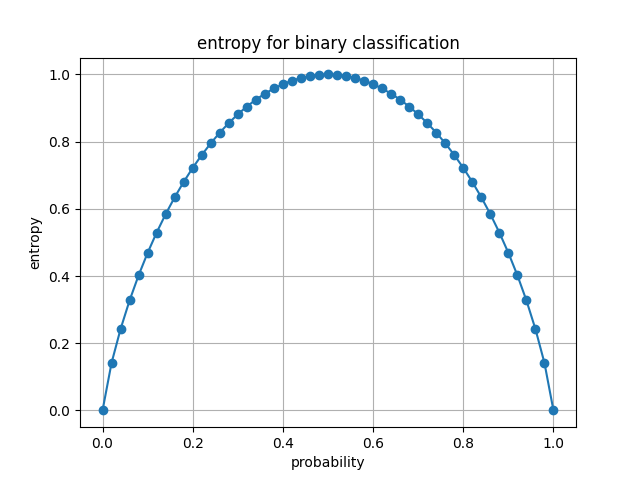
\includegraphics[scale=0.5]{pics/entroy.png}
	%{\footnotesize\textbf{Notes:} XXX.} % changed <<<<<<<<<<
	%#\label{XXX}
\end{figure}




Information gain measures the reduction in entropy that results from partitioning the data on an attribute A, which is another way of saying that it represents how effective an attribute is at classifying the data. Given a set of training data S and an attribute A, the formula for information gain is:

\begin{equation}
	Gain(S,A)  = Entropy(S) - \sum_v  \frac{|S_v|}{|S|} \; Entropy(S_v)
\end{equation}


where $v$ is all the possible values of attribute the attribute (for example, sunny, cloudy, rainy), and $S_v$ is the total number of samples corresponding to this value of attribute (for example sunny).

For \textit{if I play tennis game} (yes and no is the final output) with attributes weather (sunny, cloudy, rainy), temperature (hot, cold, mild), humidity (normal, high),  first, we calculate the entropy of the entire set (Entropy(S)) (wrt the the final output classification, yes and no). For each attribute, we calculate the the entropy corresponding to each value of entropy, then we calculate the final entropy.


We want to maximize information gain, so we want the entropies of the partitioned data to be as low as possible, which explains why attributes that exhibit high information gain split training data into relatively heterogeneous groups.

As the size of the training data and the number of attributes increase, it becomes likelier that running ID3 on it will return a sub-optimal decision tree.


The other option we can use instead of Entropy is the \textbf{Gini function.}

\hfill \break
\textbf{When do you stop splitting?}
\begin{itemize}
	\item when a node is 100\% pure
	\item when splitting a node will result in the tree exceeding a maximum depth (to avoid over-fitting)
	\item when improvement in purity score (information gain) are below a threshold
	\item when the number of examples in a node is below a threshold
\end{itemize}

\subsection{Inductive bias}
Two types of bias for classifiers:
\begin{itemize}
	\item Restriction Bias: Describes the hypothesis set space (H) that we will consider for learning the tree.
	Complete hypothesis space (low Restriction Bias). Instead of looking at infinitely many functions, we only consider those that can be represented by the decision tree.
	\item Preference Bias: Describes the subset of hypothesis n ($n \in H $), from the hypothesis set space H, that we prefer.
\end{itemize}

Inductive bias of ID3 algorithm:
\begin{itemize}
\item it prefers the decision tree with good splits at top (even if a bad split generates the same outcome). This is because ID3 is greedy using info gain.
\item it prefers correct outcome over incorrect because ID3 repeats until the labels are correctly classified.
\item it prefers shorter trees (comes from the fact that we use good splits from the top).
\end{itemize}

\subsection{Extending ID3 algorithm-other consideration}
\textbf{For continuous values attributes/features}, we can classify the attributes based on thresholds (that exists in the data set). Without threshhold, the continuous data attribute provides the most information gain, while giving a decision tree that is not generalize well. To find the threshold, we can plot the values and decide based on a threshold the returns the best outcome, by calculating the information gain values for each threshold. One way to select the threshold is to take all the values that are mid points between the sorted list of training. For example, for 10 training samples, we need to test the info gain for 9 values, for this specific feature. We can even have multiple threshold for one feature (by creating multiple features).

\textbf{Does it make sense to repeat an attribute along a path in a decision tree?} No, it does not make sense for discrete values, but for continuous values, it makes sense, because indeed we are asking a different question (for a different range).

\textbf{If the data for some attributes is missing,} see \ref{sec:missing}.

\textbf{Over-fitting + When do we stop?} When everything classified correctly or if there is no more attribute. What if we have noise in data (different answer for the same instance)? Causes an infinite loop. What would be the stopping criterion, then? We want generalization, and we should avoid \textbf{over-fitting}. If the tree is too big/complicated, there is a chance that it over-fits. There are two popular approaches to avoid over-fitting in decision trees: stop growing the tree before it becomes too large or prune the tree after it becomes too large. Typically, a limit to a decision tree’s growth will be specified in terms of the maximum number of layers, or depth, it’s allowed to have.

One option to avoid over-fitting is that we can grow the trees, and use cross-validation to prevent over-fitting. The data available to train the decision tree will be split into a training set and validation/test set and we keep growing the tree with various maximum depths will be created based on the training set and then test it against the test set. The best will be selected (when the error grows, we stop growing the tree).

Pruning the tree, on the other hand, involves testing the original tree against pruned versions of it. Leaf nodes are taken away from the tree as long as the pruned tree performs better against test data than the larger tree.


\textbf{One-hot encoding:} If there are multiple categories for a feature, we can use one-hot encoding to convert each category to a binary feature. Thus, jf a feature can take k values, one-hot encoding creates k binary features. There are libraries in the sklearn library for this task. See the details in the \ref{sec:one-hot}.

\textbf{Regression:} how to adapt decision trees for regression type of problems (continuous outputs)? Decision trees as we’ve defined them here don’t transfer directly to regression problems. We no longer have a useful notion of information gain, so our approach at attribute sorting falls through. Instead, we can rely on purely statistical methods (like variance and correlation) to determine how important an attribute is. For leaves, too, we can do averages, local linear fit, or a host of other approaches that mathematically generalize with no regard for the meaning of the data.

\subsection{Regression with Decision tree}

We can use decision trees for classification (DecisionTreeClassifier) or for regression (DecisionTreeRegressor). Training a regressor is not any different from the classifier, but for the leaf node, we use the average of the continuous values of all the samples in that node.

The major difference here is that how you choose to split the data at the node. Instead of maximizing the entropy, we try to minimize the variance of the values for the continuous feature. Thus, we calculate the variance for the values at each leaf separated by the feature, then we use a weighted method to combine it.

\begin{multline}
	\text{minimize the variance (means choose the feature with largest value)} = \\
	\text{variance of all samples at the root} - \\
	\big[ \\
	\frac{\text{num of samples in the left leaf}}{ \text{num of total samples }} \times \text{variance of left leaf} +\\
	\frac{\text{num of samples in the right leaf}}{ \text{num of total samples }} \times \text{variance of right leaf}\\
	\big]
\end{multline}



For example, if a feature divides 10 samples into two leaf nodes with 4 and 6 samples in each leaf node, then, the weighted average of variance is $\frac{4}{10} \times \text{variance of left leaf} + \frac{6}{10} \times \text{variance of right leaf} $.

\subsection{Changing the information gain formula is another option}
The information gain formula used by the ID3 algorithm treats all of the variables the same, regardless of their distribution and their importance. This is a problem when it comes to continuous variables or discrete variables with many possible values because training examples may be few and far between for each possible value, which leads to low entropy and high information gain by virtue of splitting the data into small subsets, but results in a decision tree that might not generalize well.

One successful approach to deal with this is using a formula called GainRatio in the place of information gain. GainRatio tries to correct for information gain’s natural bias toward attributes with many possible values by adding a denominator to information gain called SplitInformation. SplitInformation attempts to measure how broadly partitioned an attribute is and how evenly distributed those partitions are. In general, the SplitInformation of an attribute with n equally ­distributed values is $log_2 n$ . These relatively large denominators significantly affect an attribute’s chances of being the best attribute after an iteration of the ID3 algorithm and help to avoid choices that perform particularly well on the training data but not so well outside of it.

\begin{gather*}
	GainRatio(S,A)  = \frac{Gain(S,A)}{SplitInformation(S,A)} \\
	SplitInformation(S,A) = - \sum_{i=1}^c \frac{|S_i|}{S} \; log_2\frac{|S_i|}{|S|}
\end{gather*}


\subsection{Advantages and Disadvantages of Decision Trees (copied from a text)}
\textbf{Advantages:}

\begin{itemize}
\item Simple to understand and to interpret.
\item Requires little data preparation. Other techniques often require data normalization, dummy variables need to be created and blank values to be removed.
\item The cost of using the tree (i.e., predicting data) is logarithmic in the number of data points used to train the tree.
\item Able to handle both numerical and categorical data. Other techniques are usually specialized in analyzing datasets that have only one type of variable.
\item Able to handle multi-output problems.
\item Uses a white box model. If a given situation is observable in a model, the explanation for the condition is easily explained by Boolean logic. By contrast, in a black box model (e.g., in an artificial neural network), results may be more difficult to interpret.
\item Possible to validate a model using statistical tests. That makes it possible to account for the reliability of the model.
\item Performs well even if its assumptions are somewhat violated by the true model from which the data were generated.
\end{itemize}

\textbf{Disadvantages:}

\begin{itemize}
\item Can create over-complex trees that do not generalize the data well. This is called overfitting. Mechanisms such as pruning (setting the minimum number of samples required at a leaf node or setting the maximum depth of the tree) are necessary to avoid this problem.
\item Decision trees can be unstable because small variations in the data might result in a completely different tree being generated. This problem is mitigated by using decision trees within an ensemble (random forest/XGBoost).
\item The problem of learning an optimal decision tree is known to be NP-complete under several aspects of optimality and even for simple concepts. Consequently, practical decision-tree learning algorithms are based on heuristic algorithms such as the greedy algorithm where locally optimal decisions are made at each node. Such algorithms cannot guarantee to return the globally optimal decision tree. This can be mitigated by training multiple trees in an ensemble learner, where the features and samples are randomly sampled with replacement.
\item There are concepts that are hard to learn because decision trees do not express them easily, such as XOR, parity or multiplexer problems.
\item Decision tree learners create biased trees if some classes dominate. It is therefore recommended to balance the dataset prior to fitting with the decision tree.
\end{itemize}

\subsection{When to use a decision tree}
Decision trees and tree ensembles:
\begin{itemize}
  \item Works well on tabular/structured data
  \item Not recommended for unstructured data such as text, image, audio. Use NN here.
  \item Decision tree is fast in training.
  \item Small decision trees may be human interpretable.
\end{itemize}
Neural Networks
\begin{itemize}
  \item Works well on all types of data, including tabular/structured and unstructured data.
  \item May be slower than the decision tree for training.
  \item Works with transfer learning.
  \item When building a system of multiple models working together, it might be easier to string together multiple neural networks.
\end{itemize}


\subsection{Random forest (Tree ensembles)}
\label{sec:forest}
A single decision tree can be highly sensitive to small changes in the data.
The random forest uses many trees, and it makes a prediction by averaging the predictions of each component tree. It generally has much better predictive accuracy than a single decision tree and it works well with default parameters. If you keep modeling, you can learn more models with even better performance, but many of those are sensitive to getting the right parameters.

To build a tree ensemble (random forest), we use a technique called \textit{Sampling With Replacement}. We are going to construct random sets of the same size of the original set, that are slightly different from the original set, by randomly selecting instances from the set (so, some of the training instances might be repeated in each set). Then, we train a decision tree using this data set. We continue this process to build B decision trees (Bagged decision tree). To randomize the feature choice further, at each node, when choosing a feature to use to split, if n features are available, pick a random subset of $k<n$ features and allow the algorithm to only choose from that subset of features. If n is large $\sqrt{n}$ is valid.

\textbf{Pseudo code:} \\
Given training set of size m \\
For b=1 to B:
\begin{itemize}
  \item use sampling with replacement to create a new training set of size m
  \item train a decision tree on the new dataset
\end{itemize}

\subsection{Boosted tree (XGBoost)}
This is the most commonly used method of decision tree on samples. It requires a modification to the Bagged decision tree from the previous section \ref{sec:forest}. Basically, it is focusing on the part the data that the tree is not doing well.

\textbf{Pseudo code:}\\
Given training set of size m\\
For b=1 to B:
\begin{itemize}
  \item use sampling with replacement to create a new training set of size m
  \item \textcolor{orange}{Instead of picking from all examples with equal $1/m$ probability, make it more likely to pick misclassified examples from previously trained trees.}
  \item train a decision tree on the new dataset
\end{itemize}


\section{SL: Regression and classification}

Regression is the mapping of continuous inputs to continuous outputs, as opposed to the classification where we had mapping from discrete input to discrete output. Regression is similar to function approximation. Back then, regression meant falling  back to the average/mean, but now, we mean, using functional form to approximate a bunch of points.

We use regression because the data itself is not accurate and has noise. If the data is exact, we need to use interpolation and spline methods, to exactly fit the line with the data.

\subsection{Linear regression}

Finding a linear function/relationship between the input data and the output. It might not be a good fit though. We want to find a line (linear function) such that it minimizes the deviation, or to be more precise, the squared error between the data points and the line. This is least square regression. Basically, this is fitting data with a curve, so that we can predict the results based on the model. Here we do not try to intersect every point, rather the curve is designed to follow the pattern of points. (The other approach is interpolation that we try to pass the line/curve through each data point.)

In summary, this is an approximate function that fits the shape or general trend of the data w/o necessarily matching the individual points.
To find the line:
\begin{equation}
	\begin{split}
	\text{data points:  } \{(x_i, y_i): i=1 ... n \} \\
	\text{find a and b for the linear fit:  } y_i = a x_i + b \\
	\text{such that minimizes error:  } e = \sum_{i=1}^n (y_i -(ax_i+b))^2
	\end{split}
\end{equation}
To find the the two unknowns of the linear fit, a and b, take the derivative of the error with respect to a and b and set it zero. That would be a system of equations with two unknowns. After solving the equation you have the fit. To have a nonlinear fit, we can use a polynomial model, as discussed in the next section.

The parameters of the model are $W $ and $b$, but hyperparameters are learning rate, number of iterations, number of hidden layers, number of hidden units in each layer, the choice of activation functions, momentum, mini batch size, and regularization parameters.

To do linear regression, we can use sklearn.linear\_model.LinearRegression.

\subsection{Non-linear/polynomial regression}
\begin{equation}
	f(x_i) = a_0 + a_1 x_i + a_2 x_i^2 + ...
\end{equation}
The unknowns are $a_0, a_1, ...$.
See my class notes for more details.
To better fit the regression model, we can use higher order polynomial, but it leads to over-fitting.


\subsection{Error}
Training data has errors due to various reasons such as reading errors, sensor errors, transcription error, maliciously given data, etc. This is the reason we are using the regression not the interpolation.

To calculate the parameters of the model, we need to form the cost function (see \ref{sec:cost}) and minimize the error using an optimization technique, such as gradient descent \ref{sec:gradient}.

\subsection{Multiple Linear regression (multiple features)}

For the regression, we can have multiple independent variables/features for the regression ($x_1, ..., x_n$).

\subsection{Other cases}
Using discrete numbers is also possible for regression, however this is no trivial. We need to encode the attributes. For example, by enumerating the categories (giving a number to each possible value of this feature). It is a bit misleading because a correlation between the ordering of the
enumeration and the its value can be interpolated. The other option is represent the value of the feature as a Boolean.


\subsection{Classification}

The output variable y would be a small handful of cases (as opposed to the linear regression with infinite range of numbers). Examples of (binary) classifications, include email spam detection, tumor detection, etc.  One method is to use linear regression and map all predictions greater than 0.5 as a 1 and all less than 0.5 as a 0. This method doesn't work well because classification is not actually a linear function. Instead we need logistic regression. Logistic/Sigmoid function is (output values between 0 and 1, which is the probability of each category/class):

\begin{equation}
g(z) = \frac{1}{1+e^{-z}} \;\; \text{where} \;\; 0<g(z)<1
\end{equation}

\begin{figure}[H]
  \centering
  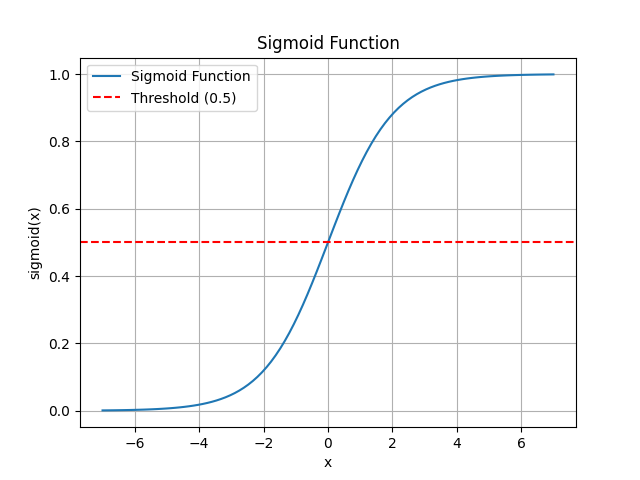
\includegraphics[trim =0.0cm 0.0cm 0.0cm 0.0cm, clip, scale=0.5]{pics/sigmoid.png}
  \caption{Sigmoid}
  %{\footnotesize\textbf{Notes:} XXX.} % changed <<<<<<<<<<
  %#\label{XXX}
\end{figure}

In the language of linear regression, it means we feed the sigmoid func with the output of linear regression:

\begin{equation}
  f_{\overrightarrow{w},b}(\overrightarrow{x}) = g(\overrightarrow{w} . \overrightarrow{x}+b)
\end{equation}

In order to get our discrete 0 or 1 classification, we can define a \textit{decision boundary}, such as 0.5, so, if $g(z) > 0.5 \rightarrow y=1$, this means $ z= \overrightarrow{w} . \overrightarrow{x}+b>0$. By setting $\overrightarrow{w} . \overrightarrow{x}+b =0$, we can find/plot the decision boundary.


\section{SL: Neural network}

Inference is getting the prediction results from a trained model using forward propagation.

\subsection{Perceptron}

Perceptron is the simplest model of a brain cell. The Perceptron calculates the sum of products of the inputs X and their corresponding weights W, and then compare the result with an activation threshold. If the sum is greater than or equal the firing threshold $\theta$, the perceptron returns one, otherwise, it is zero.

\begin{equation}
\sum_{i=1}^k X_i W_i \ge \theta  \Rightarrow y = 1 \: \text{otherwise} \: y = 0
\end{equation}

\begin{figure}[H]
	\centering
	\caption{Perceptron}
	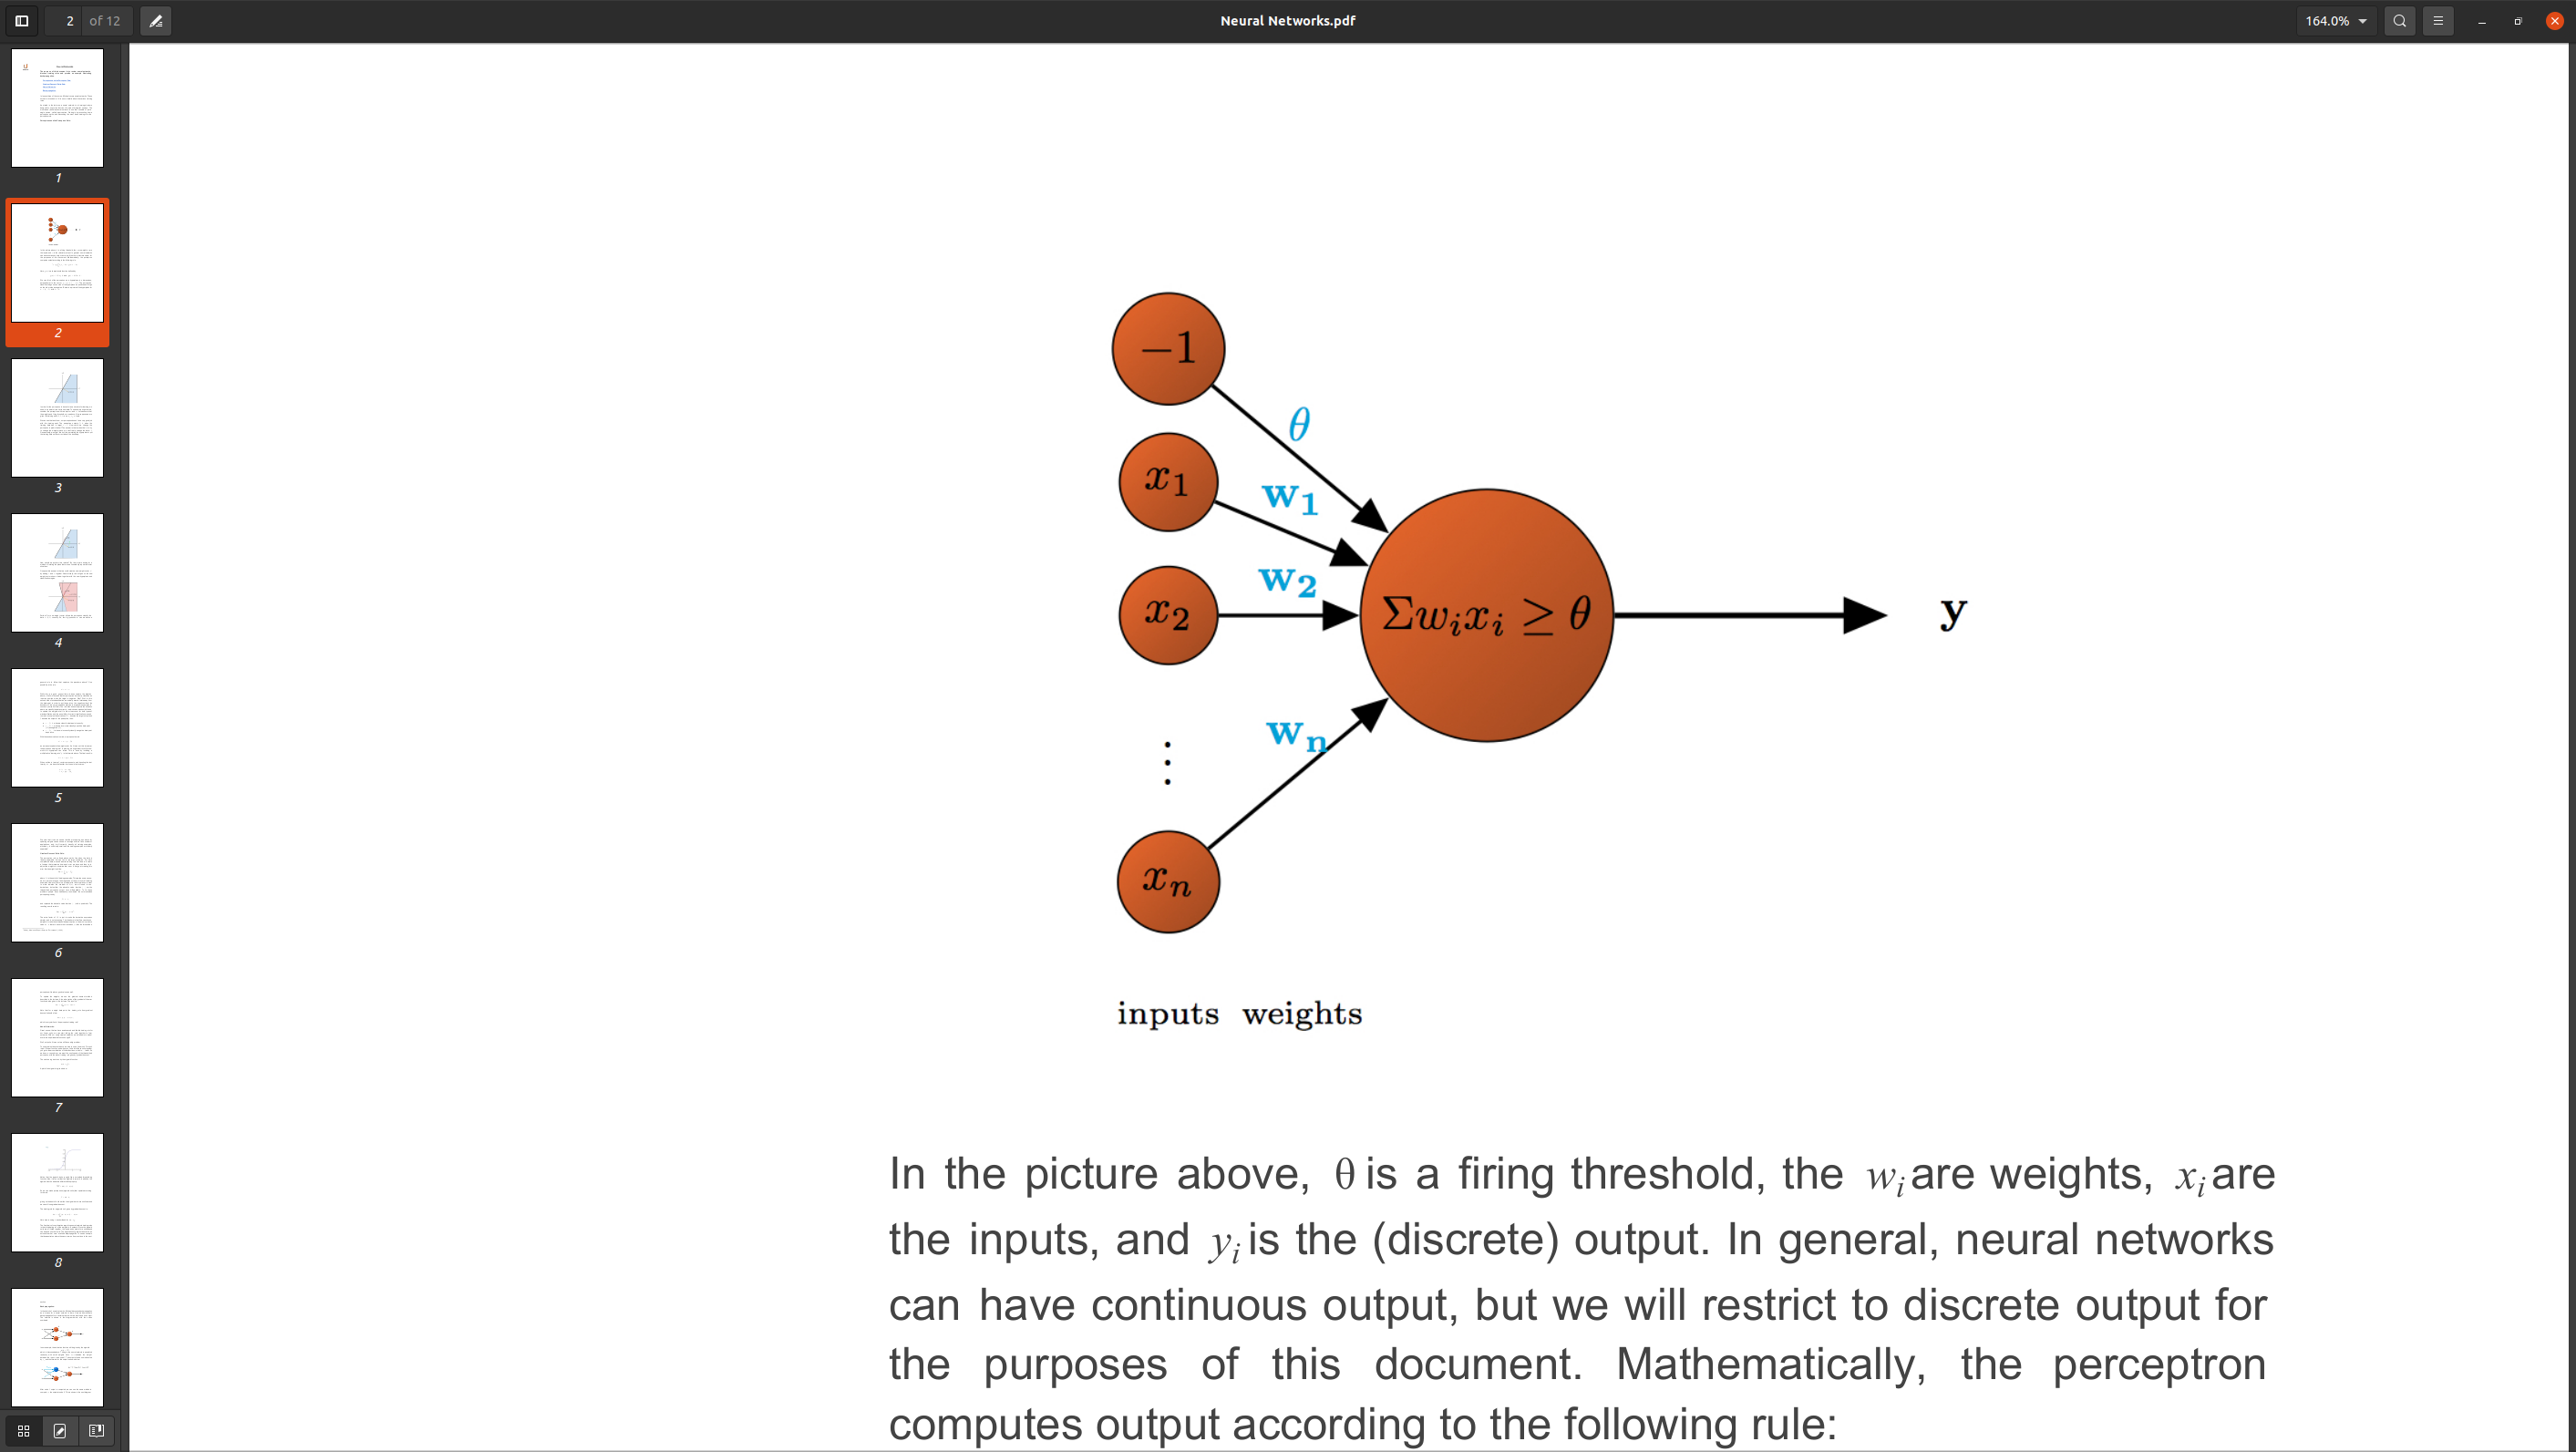
\includegraphics[trim =20cm 15.0cm 10cm 8cm, clip, scale=0.2]{pics/perceptron.png}
	%{\footnotesize\textbf{Notes:} XXX.} % changed <<<<<<<<<<
	%#\label{XXX}
\end{figure}
Layer: a group of neurons, which take the same input/features as input. A layer can have multiple or single neurons. We can assume the features as the input layer ($\overrightarrow{x}$) and the last layer as the output layer. All the layers in between (input and output) are called hidden layers.

In practice, each neuron from one layer, has access to all the neurons/inputs from the previous layer. During the training process, the weight of unrelated neurons/features becomes smaller.

Each neuron in the layer computes $\overrightarrow{w} . \overrightarrow{x}+b$ and passes the value to the next layer. Each neuron will learn a feature (such as affordability, quality, vertical line, etc.) by itself.

Each perceptron divides the space into two halves.

It is important to initialize $\overrightarrow{w}$ and $ b$ randomly, and not all equal to zero, otherwise, if all numbers are zero, there would be no training.


\subsection{Logistic regression algo with Neural Network}
We use $a$ instead of $f$, which indicate the activation function. Each neuron in a layer does this calculations. To distinguish activations/parameters for each layer, we can use superscrip []. For example, $a_2^{[1]}$ denotes the second neuron in the first layer or the same for parameters $w_2^{[1]}$. The output of layer one $a^{[1]}$ is the input for the second layer $\overrightarrow{w}^{[2]} . \overrightarrow{a}^{[1]}+b^{[2]}$. Input layer is considered as layer 0. The input layers is considered as layer 0, so $\overrightarrow{x}=\overrightarrow{a}^{[0]}$. There are several option for the activation function g() (see \ref{sec:activation}), for example, for sigmoid function, we have:

\begin{equation}
  a= f_{\overrightarrow{w},b}(\overrightarrow{x}) = g(z=\overrightarrow{w} . \overrightarrow{x}+b) = \frac{1}{1+e^{-z}}
\end{equation}

The calculation for the activation j of layer l is:

\begin{equation}
  a_j^{[l]}= g(\overrightarrow{w}_j^{[l]} . \overrightarrow{a}^{[l-1]}+b_j^{[l]})
\end{equation}

$a^{[0]}$ refers to the first layer/input layer ($X$), and the last year is  $\hat{y}= a^{[l]}$. Considering all the activation units in one layer:
\begin{equation}
  a_{n^{[l]}\times1}^{[l]}= g( z_{n^{[l]}\times1}^{[l]} = \overrightarrow{w}_{n^{[l]}\times n^{[l-1]}}^{[l]} . \overrightarrow{a}_{n^{[l-1]}\times1}^{[l-1]}+b_{n^{[l]}\times1}^{[l]})
\end{equation}

The dimension of $dW^{[l]}$ $db^{[l]}$ is the same as $W^{[l]}$ and $b^{[l]}$.

The dimension of vectorized items are ($m$ is the number of samples/training set, and $b$ is the broadcast of the same $b$ in the previous equation):
\begin{equation}
  A_{n^{[l]}\times m}^{[l]}= g( Z_{n^{[l]}\times m}^{[l]} = \overrightarrow{W}_{n^{[l]}\times n^{[l-1]}}^{[l]} . \overrightarrow{A}_{n^{[l-1]}\times m}^{[l-1]}+b_{n^{[l]}\times m}^{[l]})
\end{equation}




Why we need a deep neural network instead of a shallow one? There are functions that you can compute with a small L-layer deep neural network that shallower networks require exponentially more hidden units to compute.

Based on these notations, the forward and backward propagation look like the following plot:

\begin{figure}[H]
  \centering
  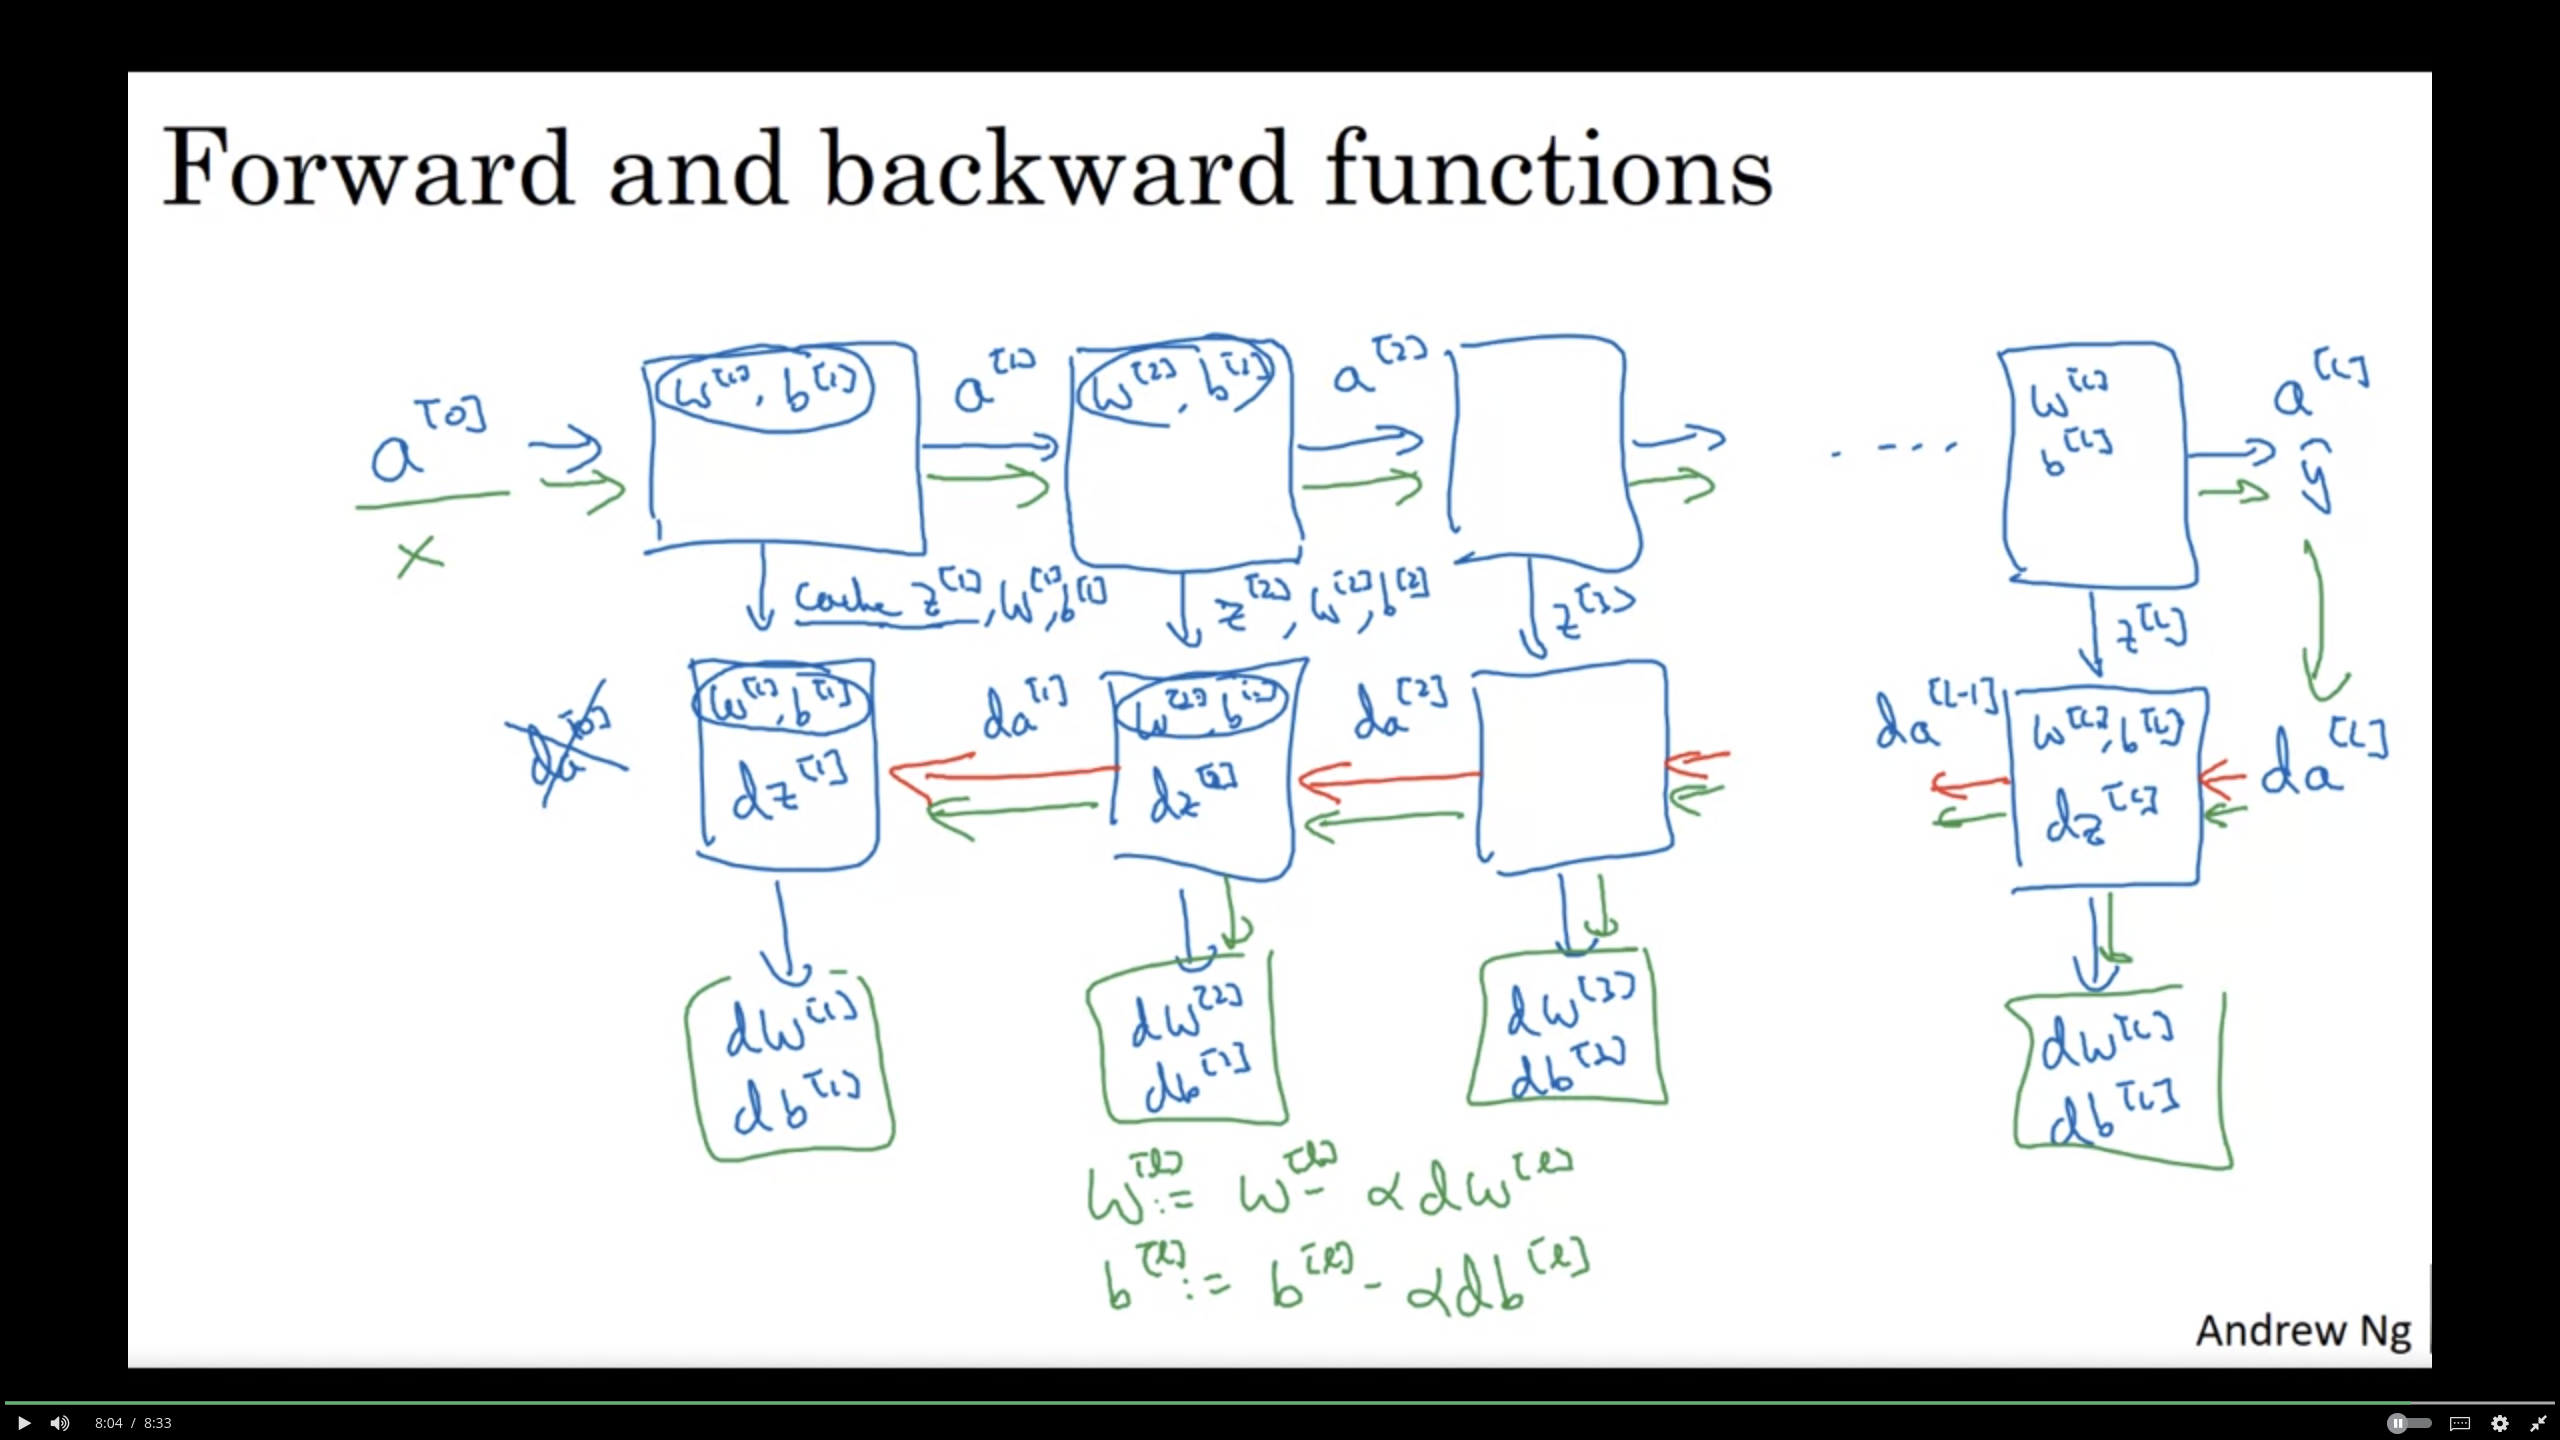
\includegraphics[trim =3.5cm 3.0cm 3.5cm 3.0cm, clip, scale=0.15]{pics/forwardbackward.png}
  \caption{Forward and Backward functions}
  %{\footnotesize\textbf{Notes:} XXX.} % changed <<<<<<<<<<
  %#\label{XXX}
\end{figure}

The backward equations look like this:
\begin{figure}[H]
  \centering
  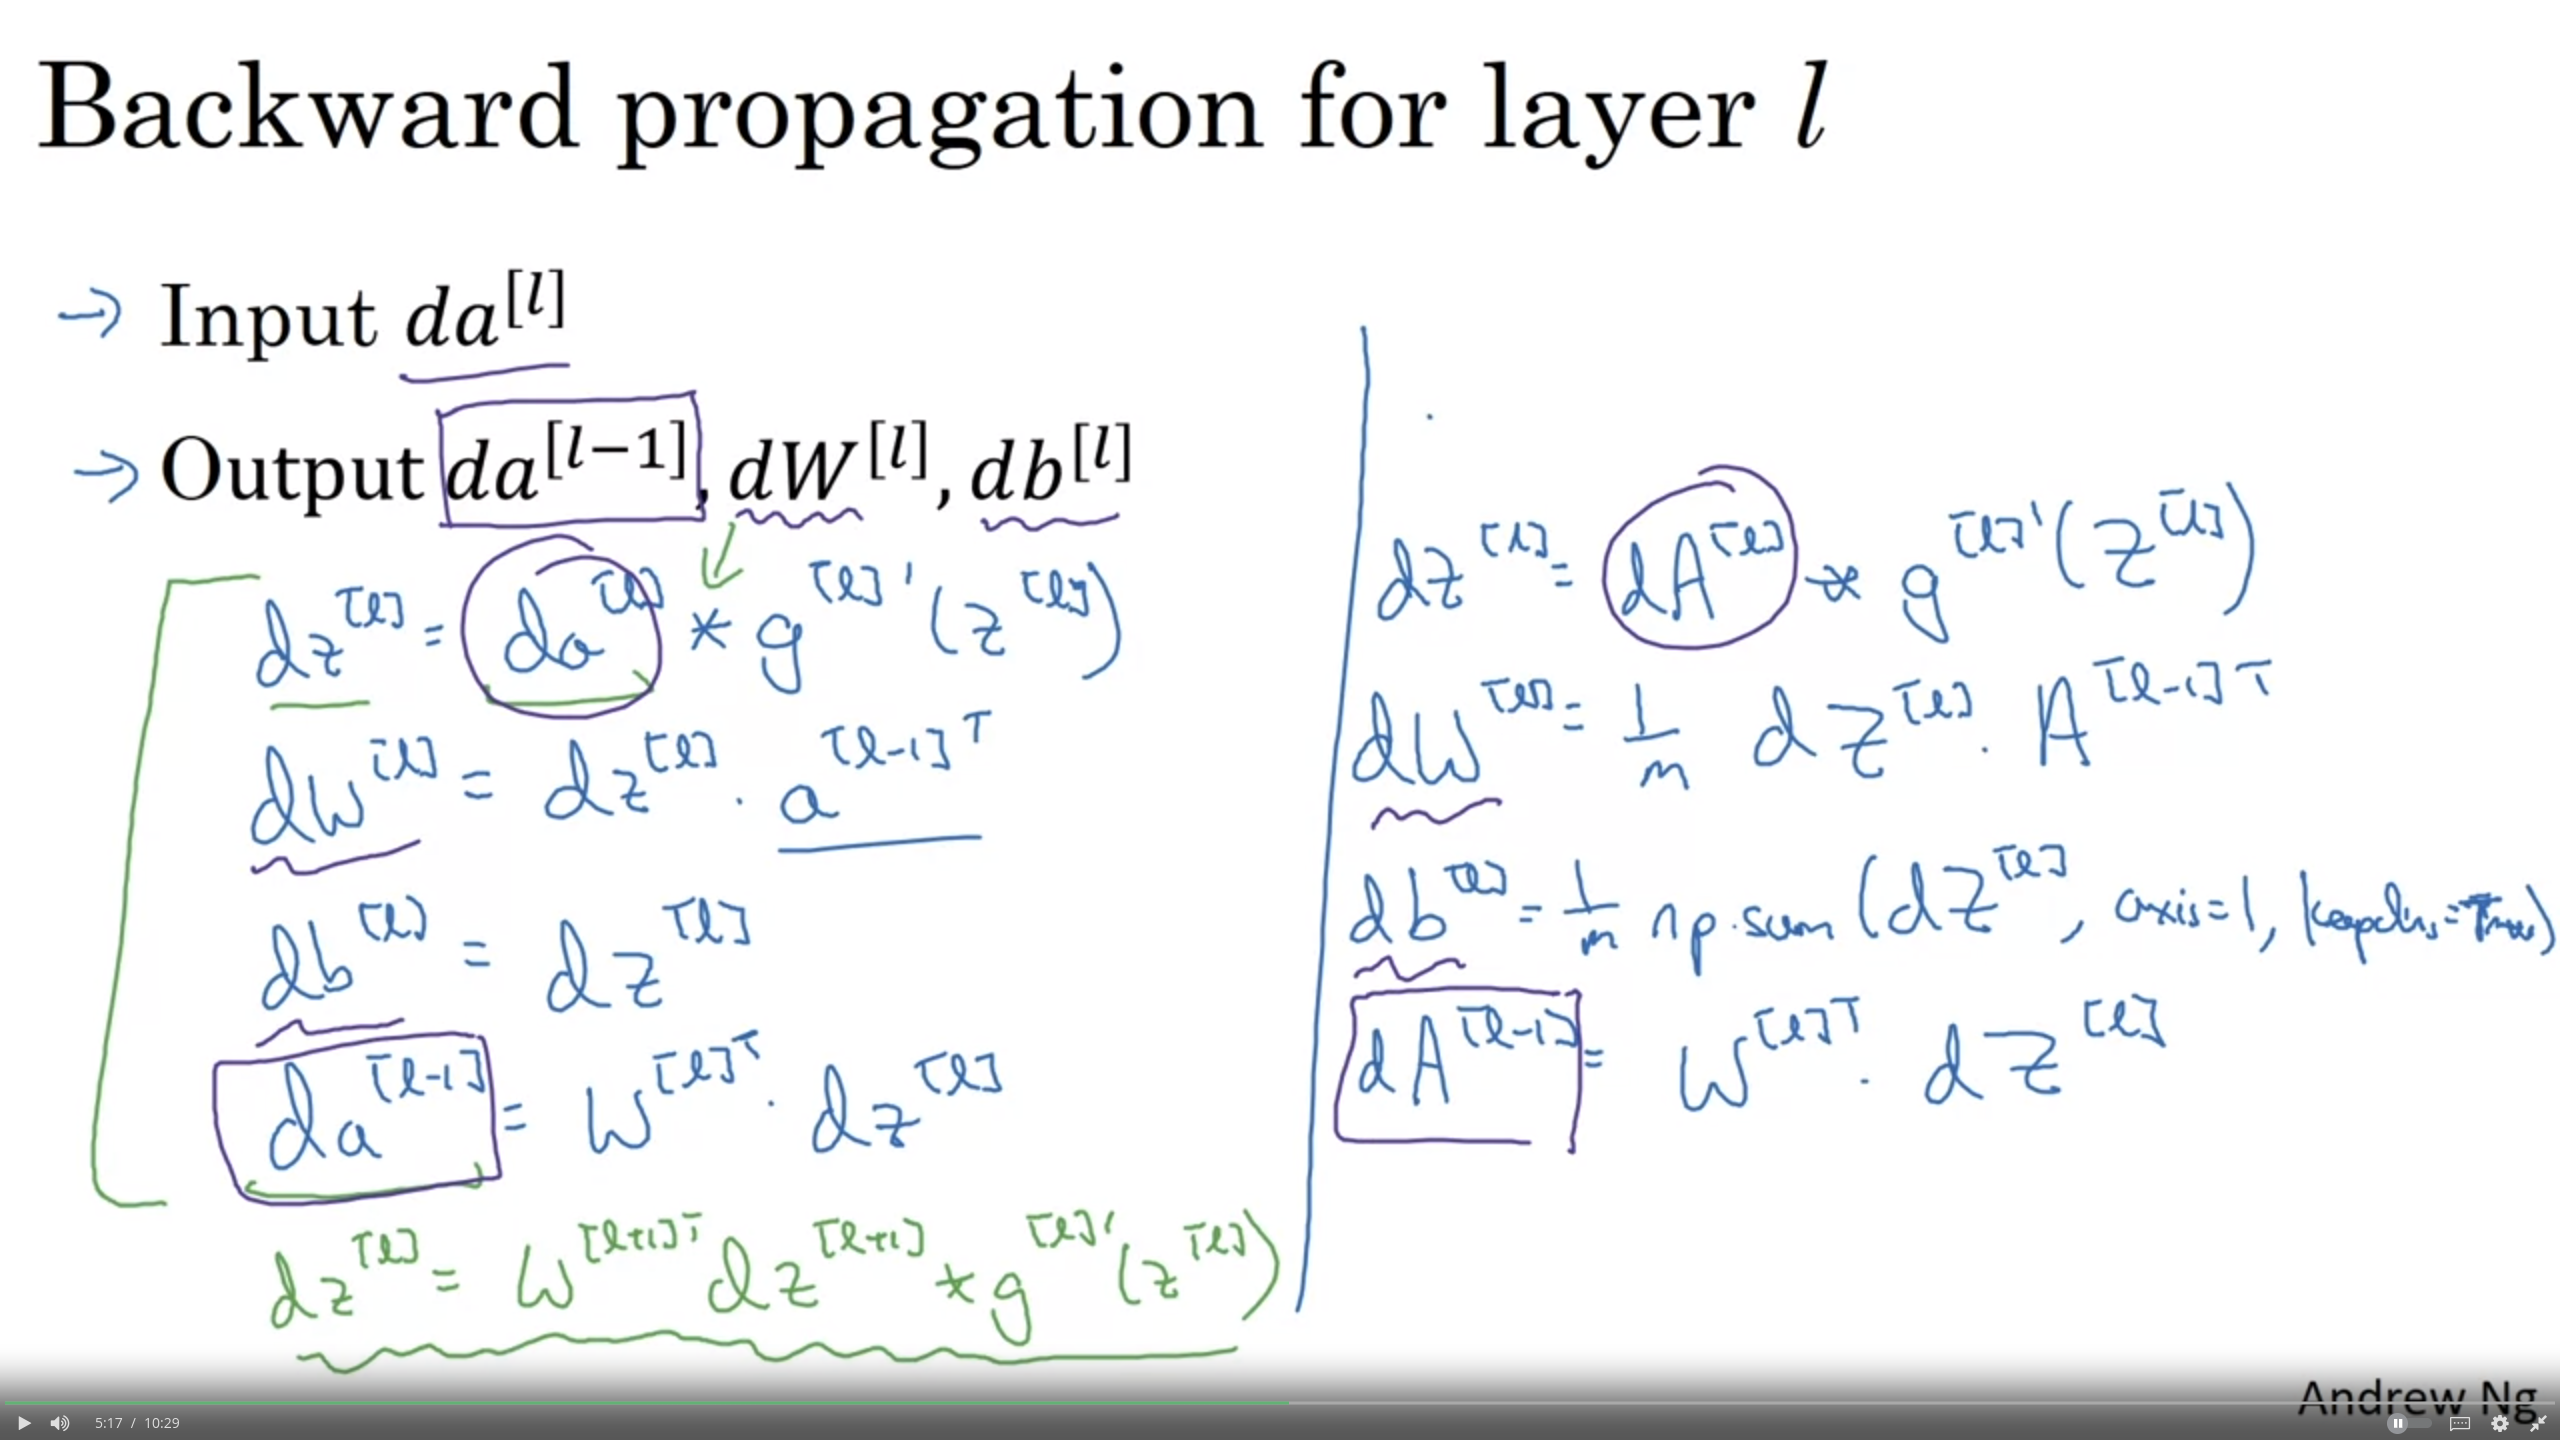
\includegraphics[trim =0.0cm 0.0cm 0.0cm 0.0cm, clip, scale=0.15]{pics/backwardeq.png}
  \caption{Forward and Backward functions}
  %{\footnotesize\textbf{Notes:} XXX.} % changed <<<<<<<<<<
  %#\label{XXX}
\end{figure}


For inference (prediction), we only need a forward propagation.

\subsection{Activation functions}
\label{sec:activation}

\textbf{Sigmoid function}, for classification:
\begin{equation}
  g(z) = \frac{1}{1+e^{-z}} \;\; \text{where} \;\; 0<g(z)<1
\end{equation}

\begin{figure}[H]
  \centering
  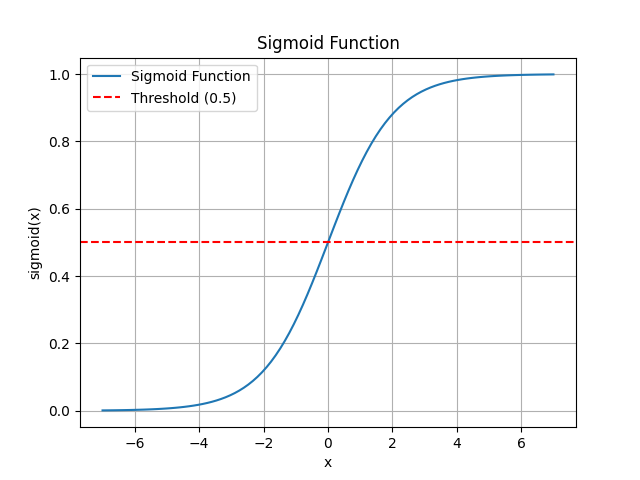
\includegraphics[trim =0.0cm 0.0cm 0.0cm 0.0cm, clip, scale=0.5]{pics/sigmoid.png}
  \caption{Sigmoid}
  %{\footnotesize\textbf{Notes:} XXX.} % changed <<<<<<<<<<
  %#\label{XXX}
\end{figure}
Since the slope is close to zero at both ends of Sigmoid function, the gradient descent becomes very slow, but with ReLU, we don't have this issue.

\textbf{Rectified Linear Unit (ReLU) function} results in any non-negative value:

\begin{equation}
  g(z) = max (0,z) =
\begin{cases}
  z \;\; z >= 0  \\
  0 \;\; z < 0 \\
\end{cases}
\end{equation}

\begin{figure}[H]
  \centering
  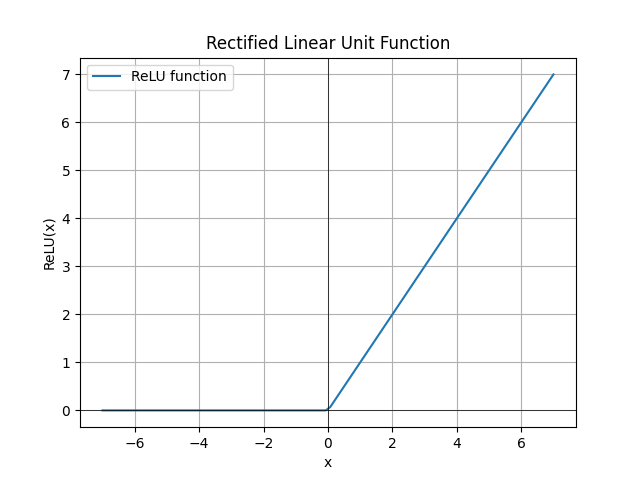
\includegraphics[trim =0.0cm 0.0cm 0.0cm 0.0cm, clip, scale=0.5]{pics/ReLU.png}
  \caption{ReLU}
  %{\footnotesize\textbf{Notes:} XXX.} % changed <<<<<<<<<<
  %#\label{XXX}
\end{figure}

\textbf{Leaky Rectified Linear Unit (ReLU) function} results in any non-negative value:
Since the derivative is zero when z is negative, we may use a small number instead of zero, which works better in practice, but rarely being used.
\begin{equation}
  g(z) = max (0,z) =
  \begin{cases}
    z \;\; z >= 0  \\
    small number \;\; z < 0 \\
  \end{cases}
\end{equation}

\begin{figure}[H]
  \centering
  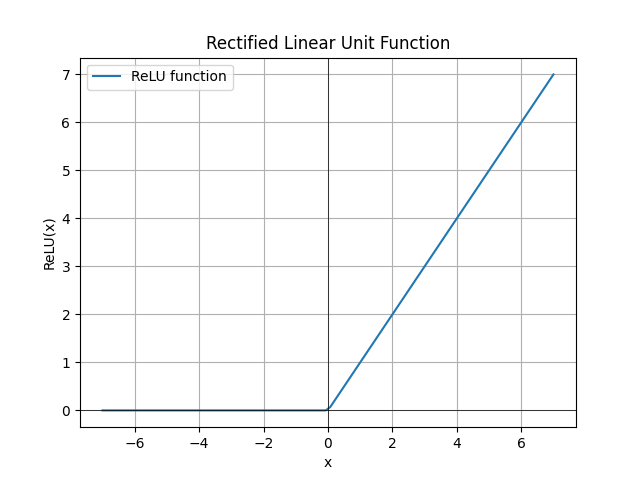
\includegraphics[trim =0.0cm 0.0cm 0.0cm 0.0cm, clip, scale=0.5]{pics/ReLU.png}
  \caption{ReLU}
  %{\footnotesize\textbf{Notes:} XXX.} % changed <<<<<<<<<<
  %#\label{XXX}
\end{figure}


\textbf{Linear function}, or in another words, not using any activation function:

\begin{equation}
  g(z) = z
\end{equation}

\begin{figure}[H]
  \centering
  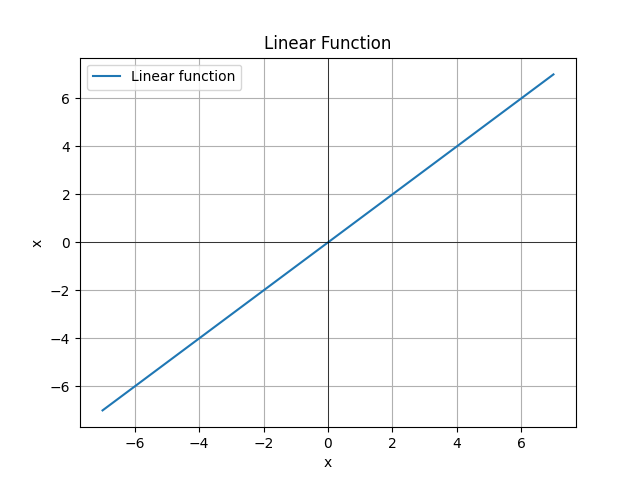
\includegraphics[trim =0.0cm 0.0cm 0.0cm 0.0cm, clip, scale=0.5]{pics/Linear.png}
  \caption{Linear function}
  %{\footnotesize\textbf{Notes:} XXX.} % changed <<<<<<<<<<
  %#\label{XXX}
\end{figure}

\textbf{Multiclass classification} refers to classification problems where you can have more than just two possible output labels. The last layer has m activation units, corresponding to the m required classes, where each output is associated with a category/class.

\textbf{Softmax function} is a generalization of the logistic function. The last layer generates a vector of size m by a linear function which is applied to a softmax function. The softmax function converts the last layer into a probability distribution as described below. After applying softmax, each output will be between 0 and 1 and the outputs will add to 1, so that they can be interpreted as probabilities. The larger inputs will correspond to larger output probabilities. It provides probabilities of the input being in each category.


The last layer, then, has m activation units, each of which calculated as:

\begin{equation}
  a_i = \frac{e^{z_i}}{ \sum_{j=1}^{m} e^{z_j} } \;\; \text{where} \;\; z_i= \overrightarrow{w}_i. \overrightarrow{x}+b_j
\end{equation}
Note that $\sum_{i = 1}^{m}  a_i = 1$

The name softmax is coming from the contrast function hard-max, which converts the last year, to a vector with only one true / 1 label, and the rests would be zero. But with the softmax, all elements have a value and the sum of all values are one. Note also that if number of softmax classes is two, the softmax reduces to logistic regression.


Tanh function, LeakyReLU function, and swish function are other choices.


\textbf{Multi-label classification} (different from multiclass classification): for example, in image processing we want to know if there is a bus/car/pedestrian. One way to have three model/NN for each label. The other way is to train one model/NN to simultaneously detect all three. For that, the last layer should have three units with a sigmoid function for each of those last year units.


\textbf{How to select activation function?}
The selection of activation function for the final/output layer, depends on the type of target. For example for binary classification, we need sigmoid. For regression, we can use linear activation function. If the target is a positive number, such as the price of a house, ReLU is the natural choice.

For hidden layers though, ReLU is a better choice. The reason is that ReLU function is faster to computer. Next reason is that ReLU is only flat in one side of the function but sigmoid is flat on both sides, which makes gradient descend very slow.



\textbf{Why do we need activation function?}
A neural network with no activation function is exactly the same as a linear regression method, and multiple layers is not helping to improve the neural net.  To create non-linearity in the cost function.

\subsection{Biases}

What kind of problems are neural networks appropriate for solving?

\textbf{Restriction Bias} A neural network’s restriction bias (which, if you recall, is the representation’s ability to consider hypotheses) is basically non-existent if you use sigmoids, though certain models may require arbitrarily-complex structure. We can clearly represent Boolean functions with threshold-like units. Continuous functions with no “jumps” can actually be represented with a single hidden layer. We can think of a hidden layer as a way to stitch together “patches” of the function as they approach the output layer. Even arbitrary functions can be approximated with a neural network! They require two hidden layers, one stitching at seams and the other stitching patches.

This lack of restriction does mean that there’s a significant danger of overfitting, but by carefully limiting things that add complexity (as before, this might be layers, nodes, or even the weights themselves), we can stay relatively generalized.


\textbf{Preference Bias} On the other hand, we can’t yet answer the question of the pref-
erence bias of a neural network (which, if you recall, describes which hypotheses from
the restricted space are preferred). We discussed the algorithm for updating weights
(gradient descent), but have yet to discuss how the weights should be initialized in the first place.

Common practice is choosing small, random values for our initial weights. The randomness allows for variability so that the algorithm doesn’t get stuck at the same local minima each time; the smallness allows for relative adjustments to be impactful and reduces complexity. Given this knowledge, we can say that neural networks—when all other things are equal—prefer simpler explanations to complex ones. This idea is an embodiment of Occam’s Razor: Entities should not be multiplied unnecessarily. More colloquially, it’s often expressed as the idea that the simpler explanation is likelier to be true.




\subsection{Convolutional Neural Network (CNN)}
In this method, each neuron only looks at part of the previous layer's outputs, instead of a regular layer, which each neuron has weights for all previous layer neurons. The main advantage of this method is that 1) it is faster, 2) Need less training data and less prone to overfitting.

\subsection{Tuning hyperparameters}

\begin{itemize}
  \item learning rate (most important parameter \#1) $\alpha$
  \item momentum term  (\#2)$\beta$
  \item Adam optimization $\beta_1, \beta_2, \epsilon$ (\#4)
  \item number of layers (\#3)
  \item number of units in each layer (\#2)
  \item learning rate decay (\#3)
  \item mini-batch size (\#2)
\end{itemize}

To investigate the hyperparameters, use random points rather than a grid. You may need to test these with many hyperparamters simultaneously. The other technique is to go from a coarse to fine regions.

Using an appropriate scale to pick hyperparamters matters, for example, for number of layers/units, we can use an equally spaced grid or linear scale, but for the learning rate we need to use logarithmic pattern ($\alpha = 10^{-4 \times np.random.rand()}$).

For exponentially weighted average, we can use $1-\beta$, sample uniformly between 0.1 to 0.001 $\beta = 1-10^{-3 \times np.random.rand()}$.

Some of the hyperparameters have independent effects on the outcome. This is called orthogonalization. Experts know what knob to turn, to get what they want in a model. Here is the chain of assumptions in ML:
\begin{itemize}
  \item fit training set well on cost function (human-level performance). If not working well:
  \begin{itemize}
    \item use a bigger network
    \item use more efficient optimization, such as Adam
  \end{itemize}
  \item fit dev set well on cost function. if not working well:
  \begin{itemize}
    \item use regularization
    \item use bigger training set
  \end{itemize}
  \item fit test set well on cost function. if not working well:
  \begin{itemize}
    \item use bigger dev set
  \end{itemize}
  \item performs well in real world
  \begin{itemize}
    \item change dev set
    \item change cost function
  \end{itemize}
\end{itemize}

Early stopping method might not be good option.

\subsection{Error analysis}

Deep learning models are quite robust to random errors in the training set, but very sensitive to the systematic errors.

\section{SL: Sequence models-Recurrent Neural Network (RNN)}

RNN is a neural network that deals with the different amount of inputs. Similar to the regular NN, RNN has bias, weights, and activation functions. The only difference is that RNN has feedback loops, which allows prior values influence the prediction. Examples of sequence data with different amount of input: stock market predictions, speech recognition, music generation, sentiment classification, DNA sequence analysis, machine translation, video activity recognition, and name entity recognition (finding the names in a sentence).

The main idea is that we have the same NN, and for each each input we repeat/unroll the same NN and add the output from the previous input/NN to the next one. Regardless of how many times we unroll the neural network, weights and biases are shared across every input. One mathematical issue with the RNN is the \textbf{\textit{vanishing/exploding gradient problem}}. As the number of input increases, if the weight is greater than one, we keep multiplying, until the number explodes, and this results is very large steps in the gradient descent.  The same way, if weights are less than one, after some multiplication, the number vanishes, and in the gradient descent, this results in very small steps.

The downside of RNN is that it only uses the info before the current layer (This is for unidirectional method, in the bidirectional, we move in both directions). Here is the forward propagation:

\begin{figure}[H]
  \centering
  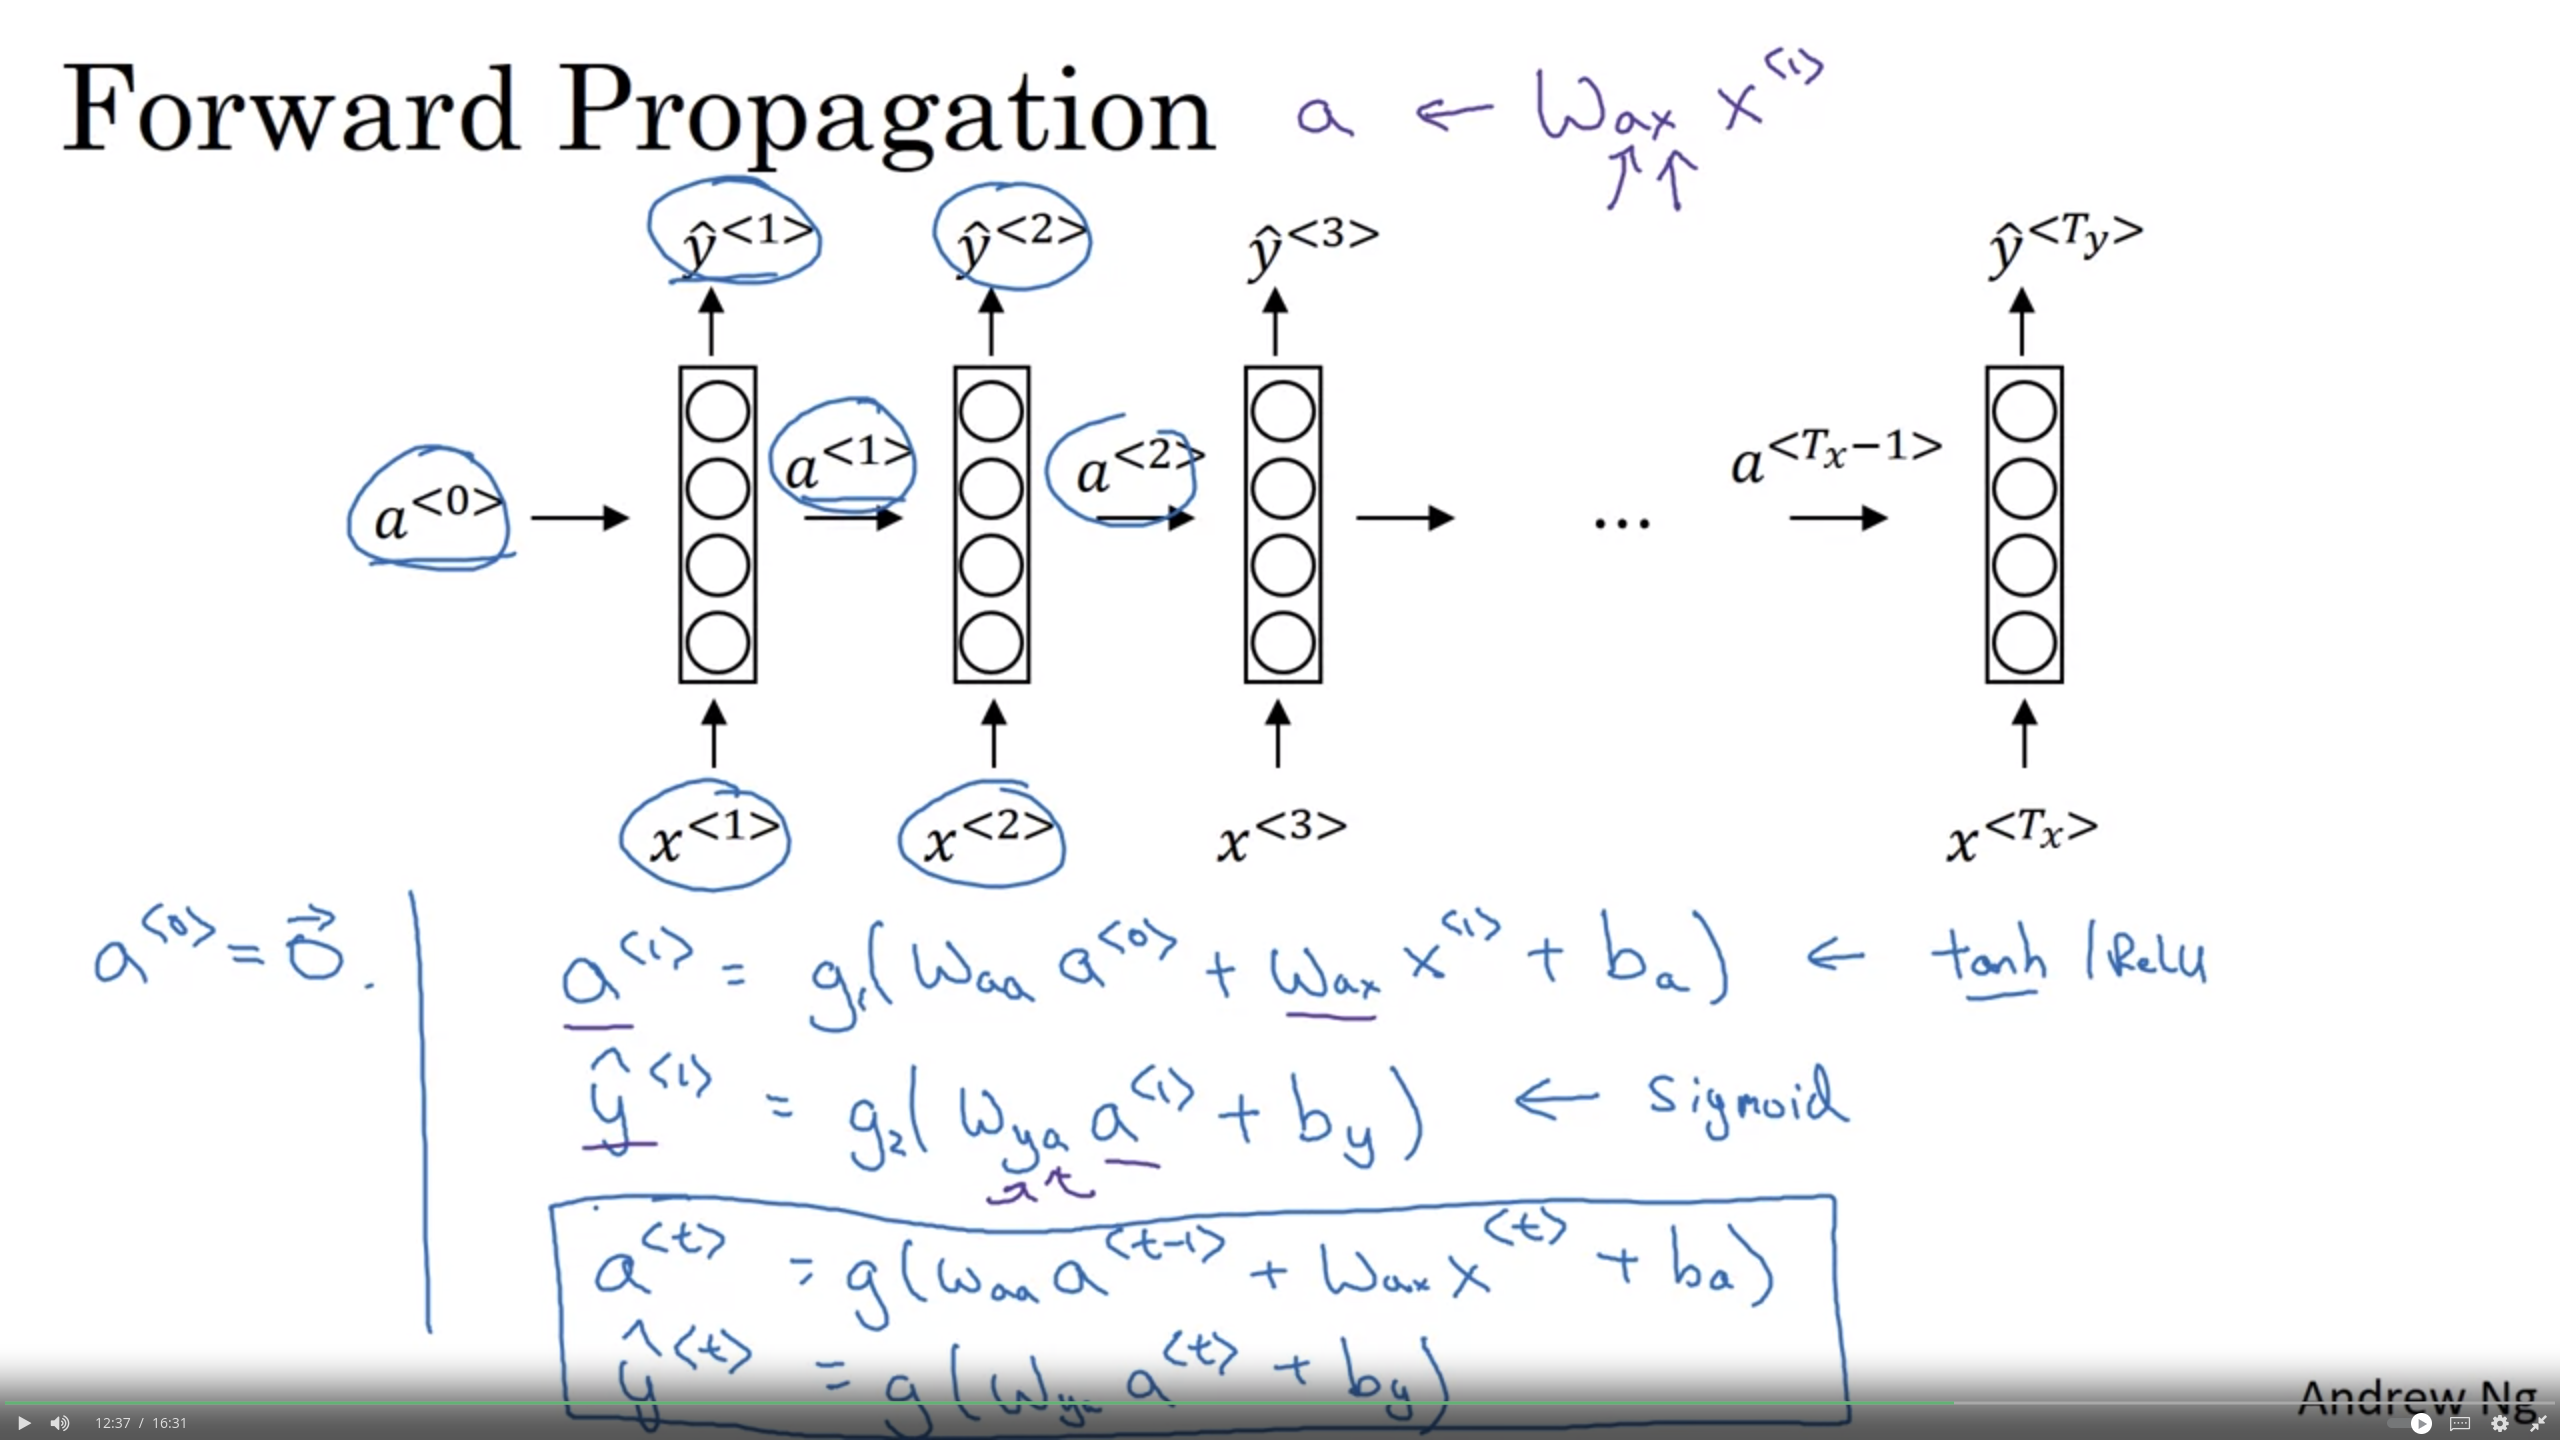
\includegraphics[trim =0.0cm 0.0cm 0.0cm 0.0cm, clip, scale=0.15]{pics/RNN.png}
  \caption{Forward propagation chart for RNN}
  %{\footnotesize\textbf{Notes:} XXX.} % changed <<<<<<<<<<
  %#\label{XXX}
\end{figure}

Here is the backpropagation model:

\begin{figure}[H]
  \centering
  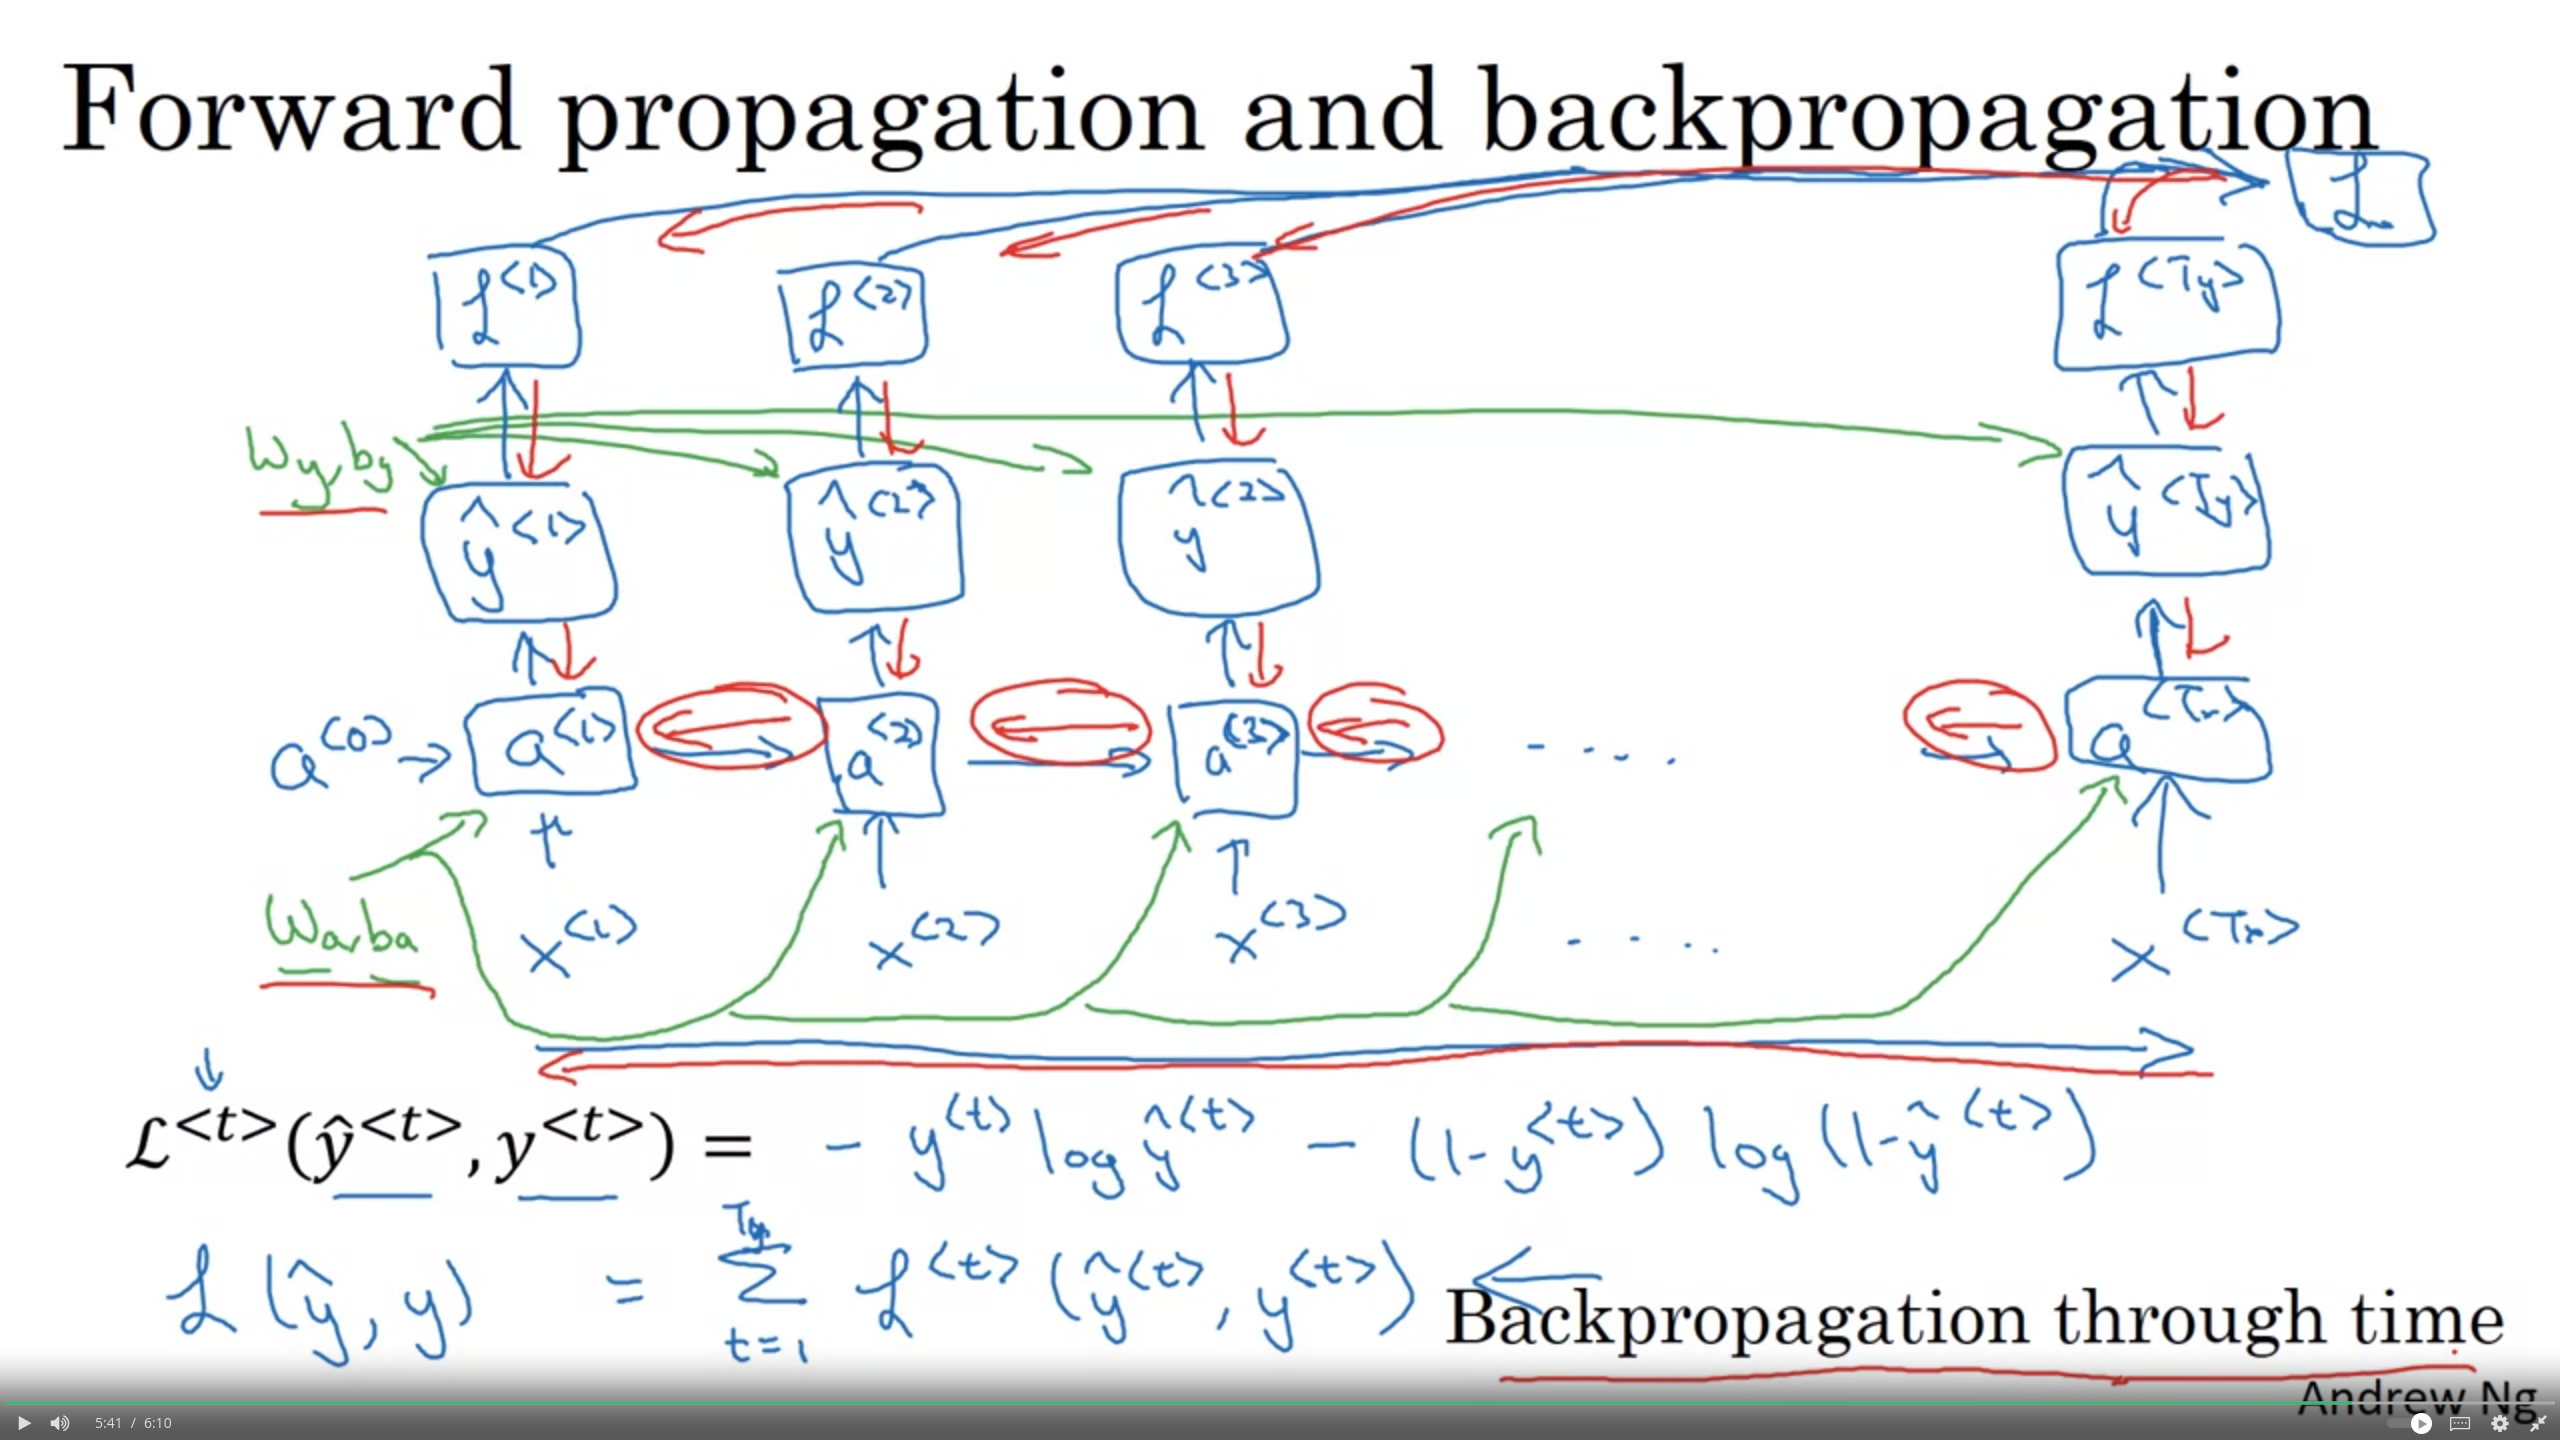
\includegraphics[trim =0.0cm 0.0cm 0.0cm 0.0cm, clip, scale=0.15]{pics/RNNback.png}
  \caption{Back propagation chart for RNN}
  %{\footnotesize\textbf{Notes:} XXX.} % changed <<<<<<<<<<
  %#\label{XXX}
\end{figure}

There are five different types of RNN model, as depicted in the following figure:
\begin{figure}[H]
  \centering
  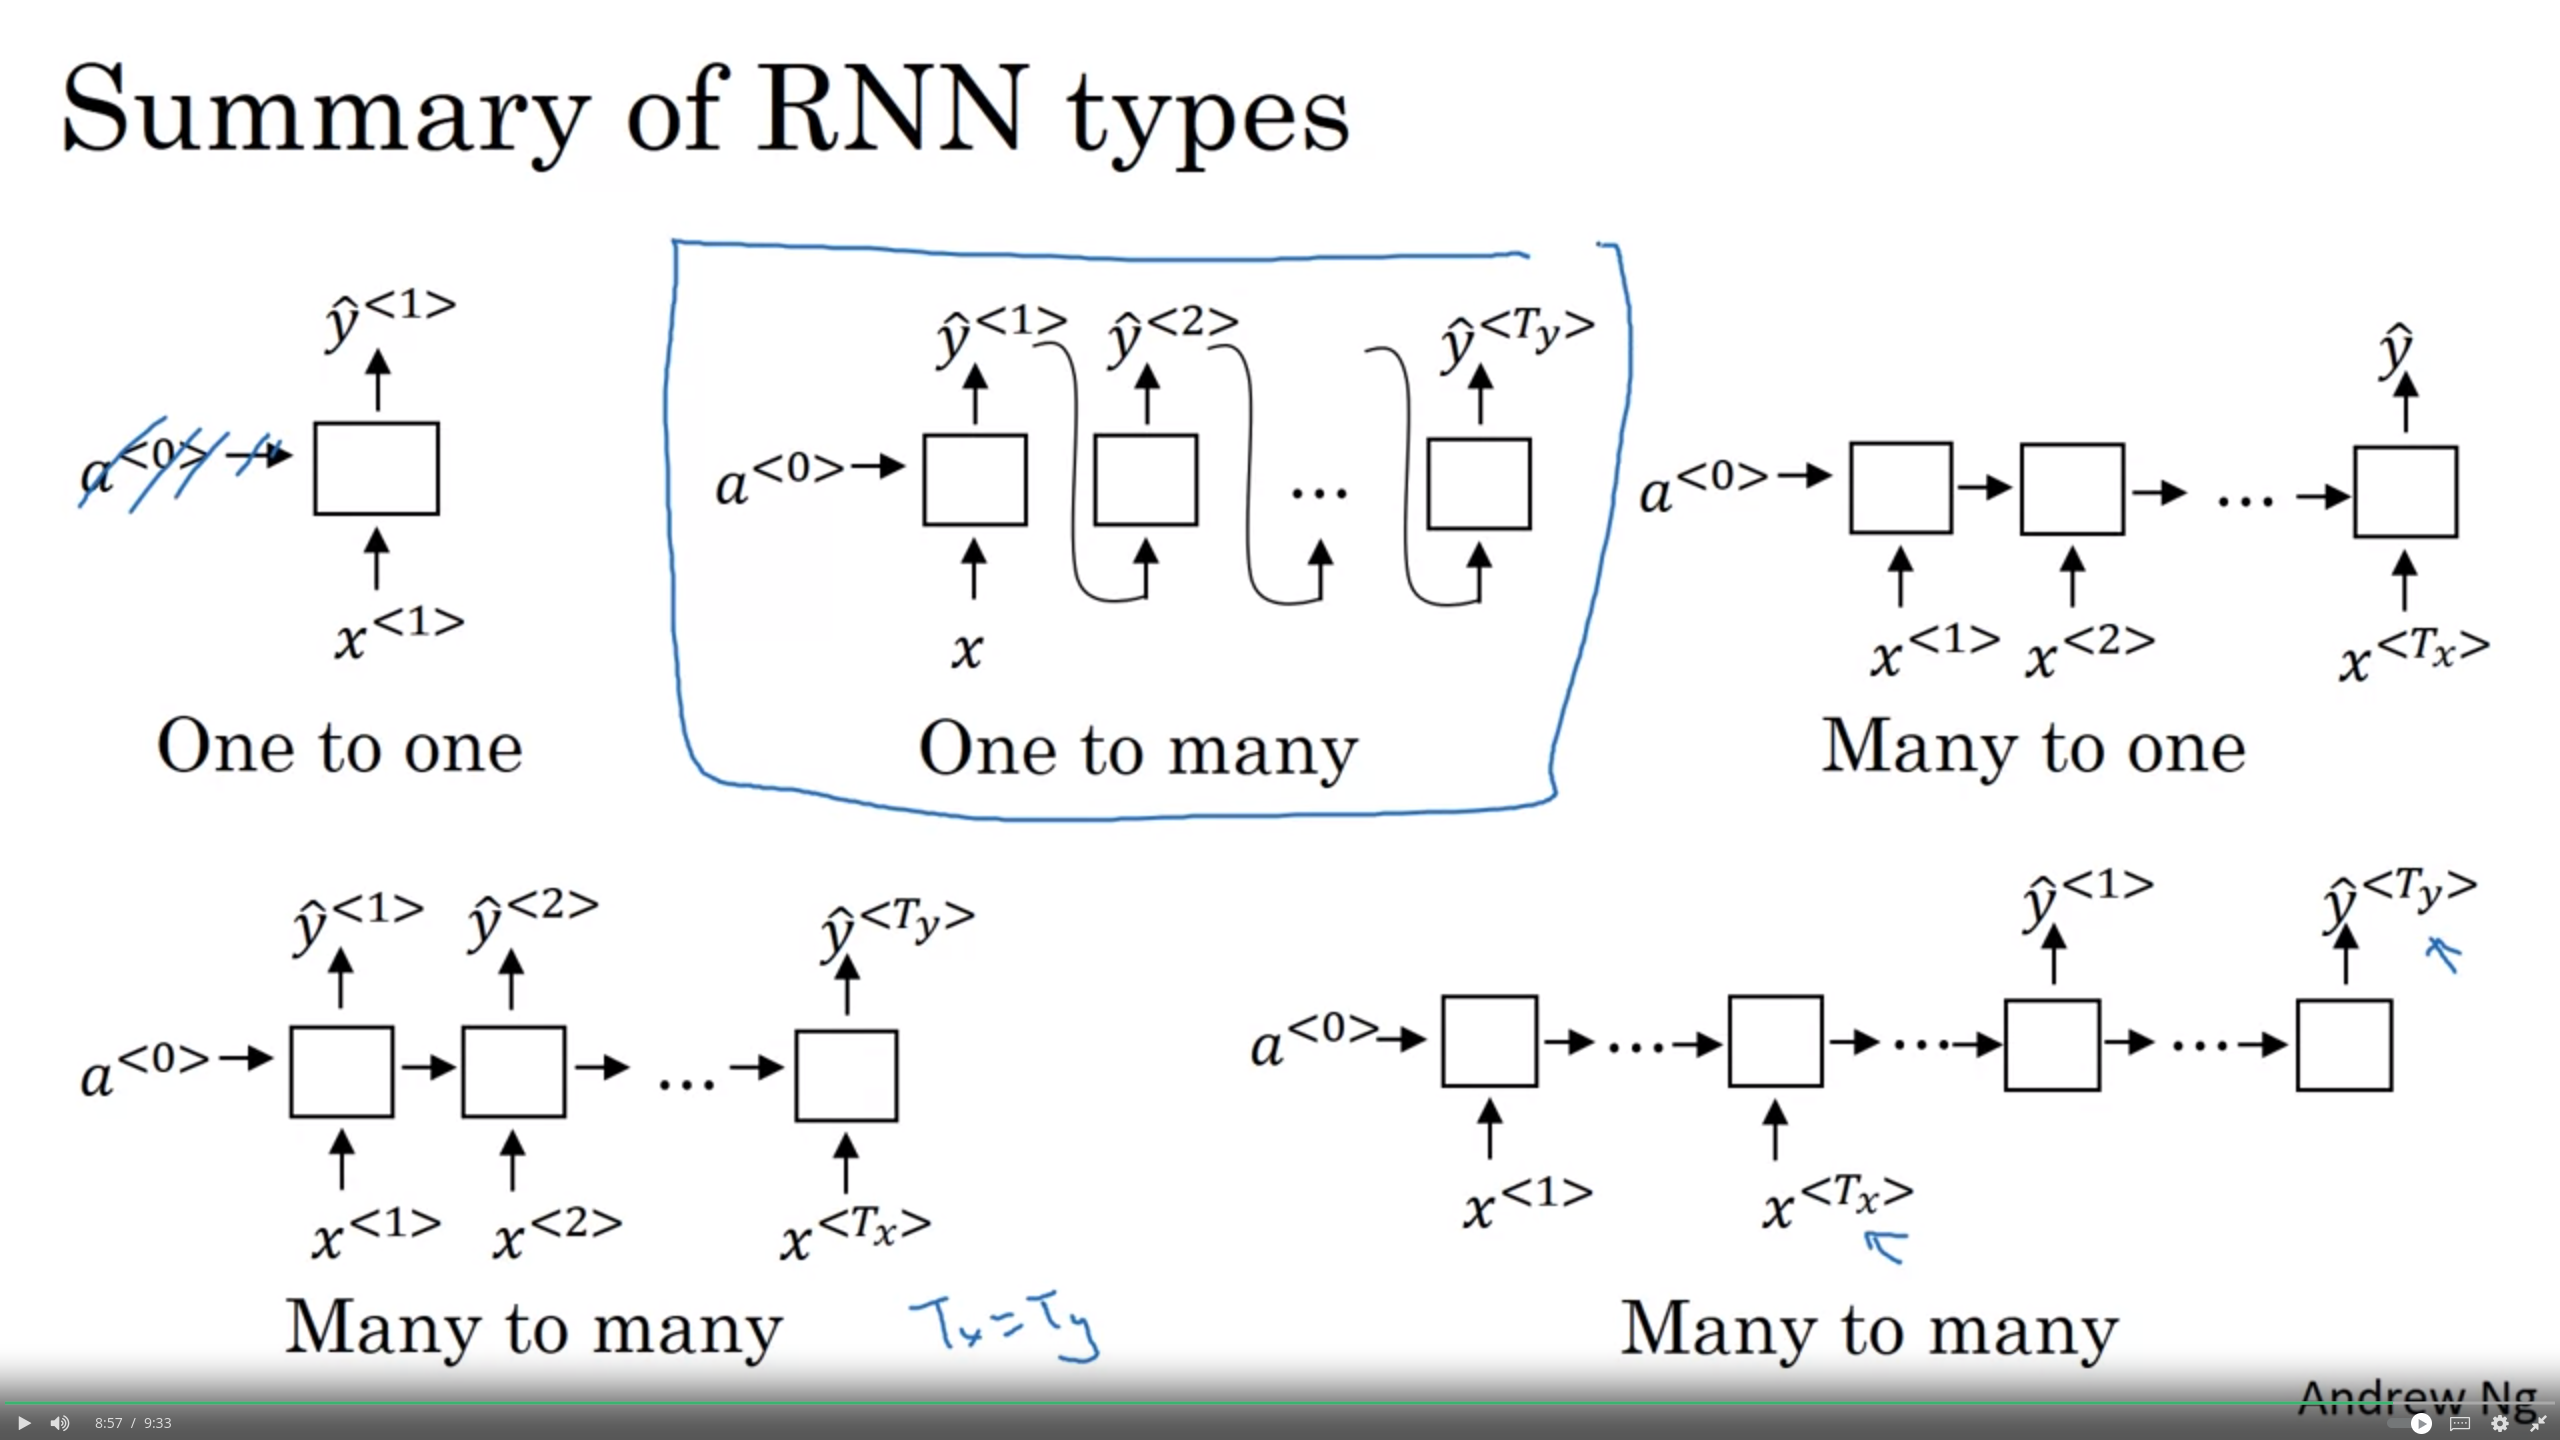
\includegraphics[trim =0.0cm 0.0cm 0.0cm 0.0cm, clip, scale=0.15]{pics/RNNtypes.png}
  \caption{Various RNN types}
  %{\footnotesize\textbf{Notes:} XXX.} % changed <<<<<<<<<<
  %#\label{XXX}
\end{figure}



One main application of the DRNN is in NLP models. There is a dictionary/vector with all the words, and each word of the sentence is translated to a one-hot vector of the size of the dictionary, with all zeros, except for the index of the word which is one. Then, each sentence is a matrix where the number of columns is equal to the number of words in the sentence. For the words that are not in the dictionary, we can add one token to the dictionary for unknown words. Since every sentence has a different length, we cannot just train a regular NN.


From chatGPT: which ML model is used for LLM:
"
Transformer-based architectures, including those used in large language models like GPT, are not based on Recurrent Neural Networks (RNNs). Instead, they rely on a different architecture known as the transformer.

RNNs are sequential models that process input data one element at a time while maintaining an internal state that represents information from previous elements. While RNNs have been widely used in natural language processing tasks, they have limitations in capturing long-range dependencies due to the sequential nature of their computation and the vanishing gradient problem.

Transformers, on the other hand, are designed to handle sequential data more efficiently by employing self-attention mechanisms. This allows them to capture relationships between different elements of the input sequence simultaneously, making them better suited for tasks involving long-range dependencies. Transformers have gained popularity in recent years due to their superior performance on various natural language processing tasks, including language modeling, machine translation, and text generation.
"

Vanishing and exploding gradients are major challenges of RNN. One way to avoid that is Gated Recurrent Unit (GRU).

\begin{figure}[H]
  \centering
  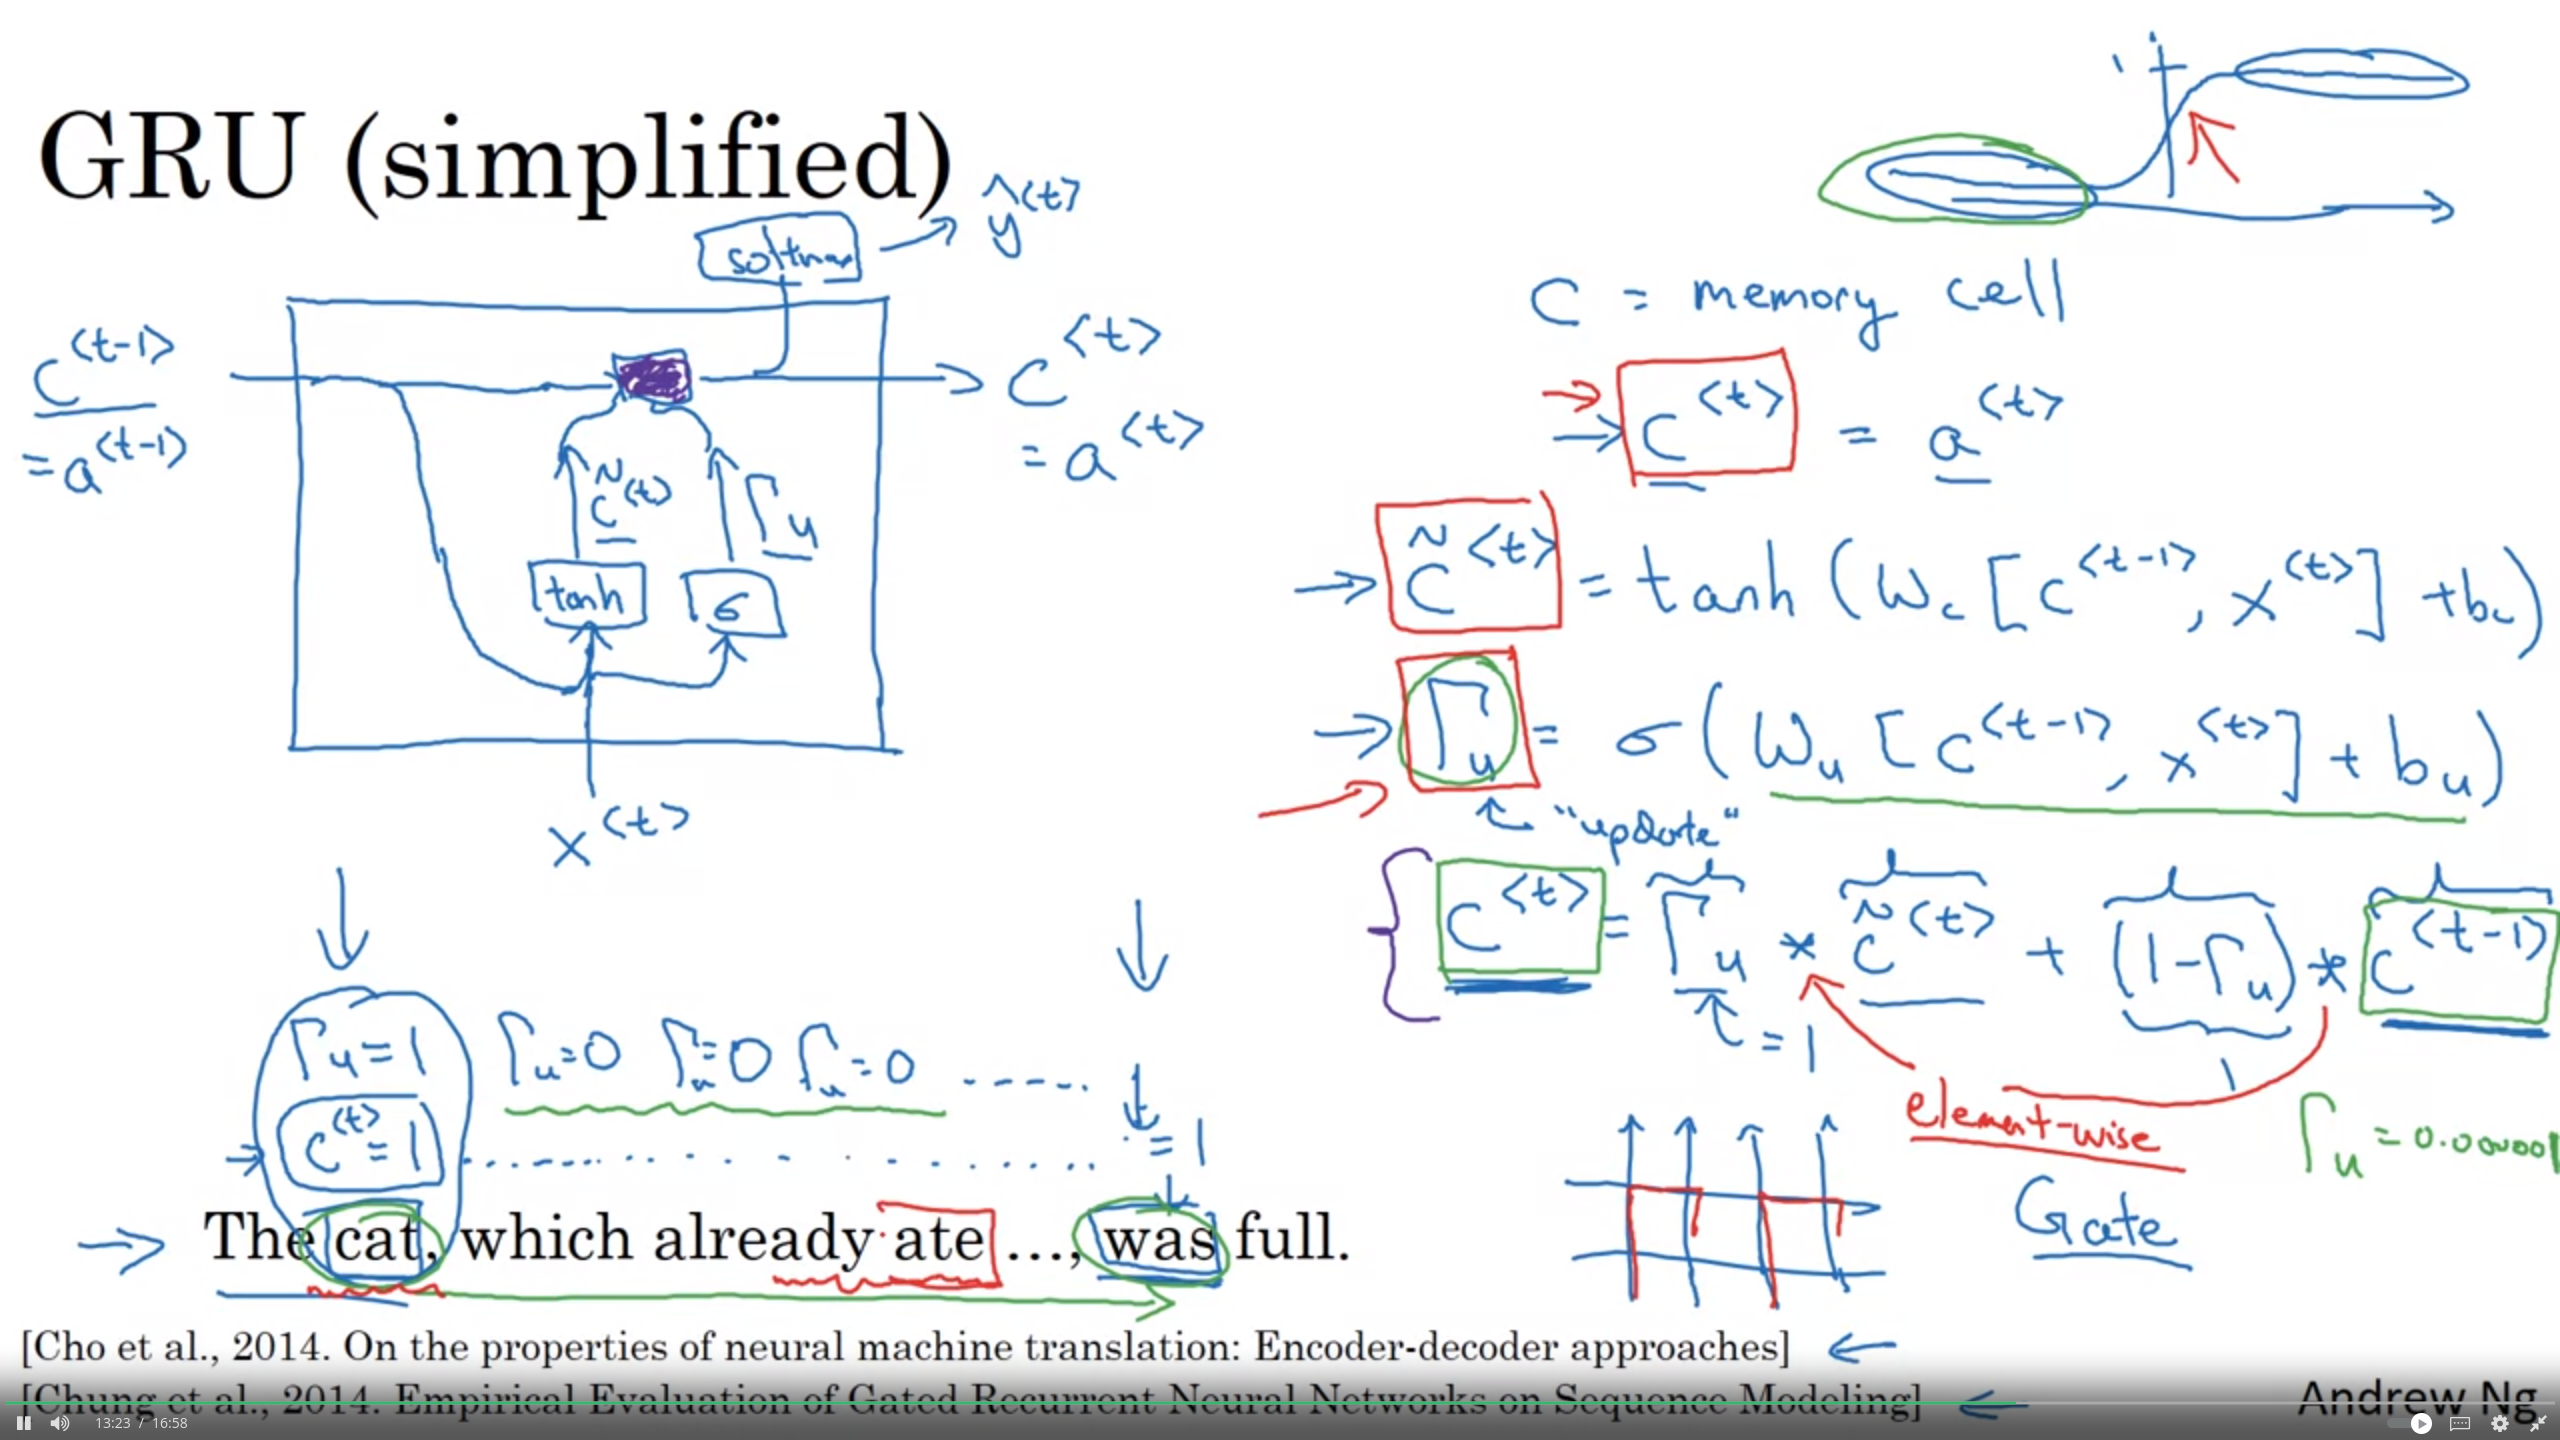
\includegraphics[trim =0.0cm 0.0cm 0.0cm 0.0cm, clip, scale=0.15]{pics/RNNGRU.png}
  \caption{Various RNN types}
  %{\footnotesize\textbf{Notes:} XXX.} % changed <<<<<<<<<<
  %#\label{XXX}
\end{figure}

Long Short-Term Memory (LSTM) is similar to GRU,

\begin{figure}[H]
  \centering
  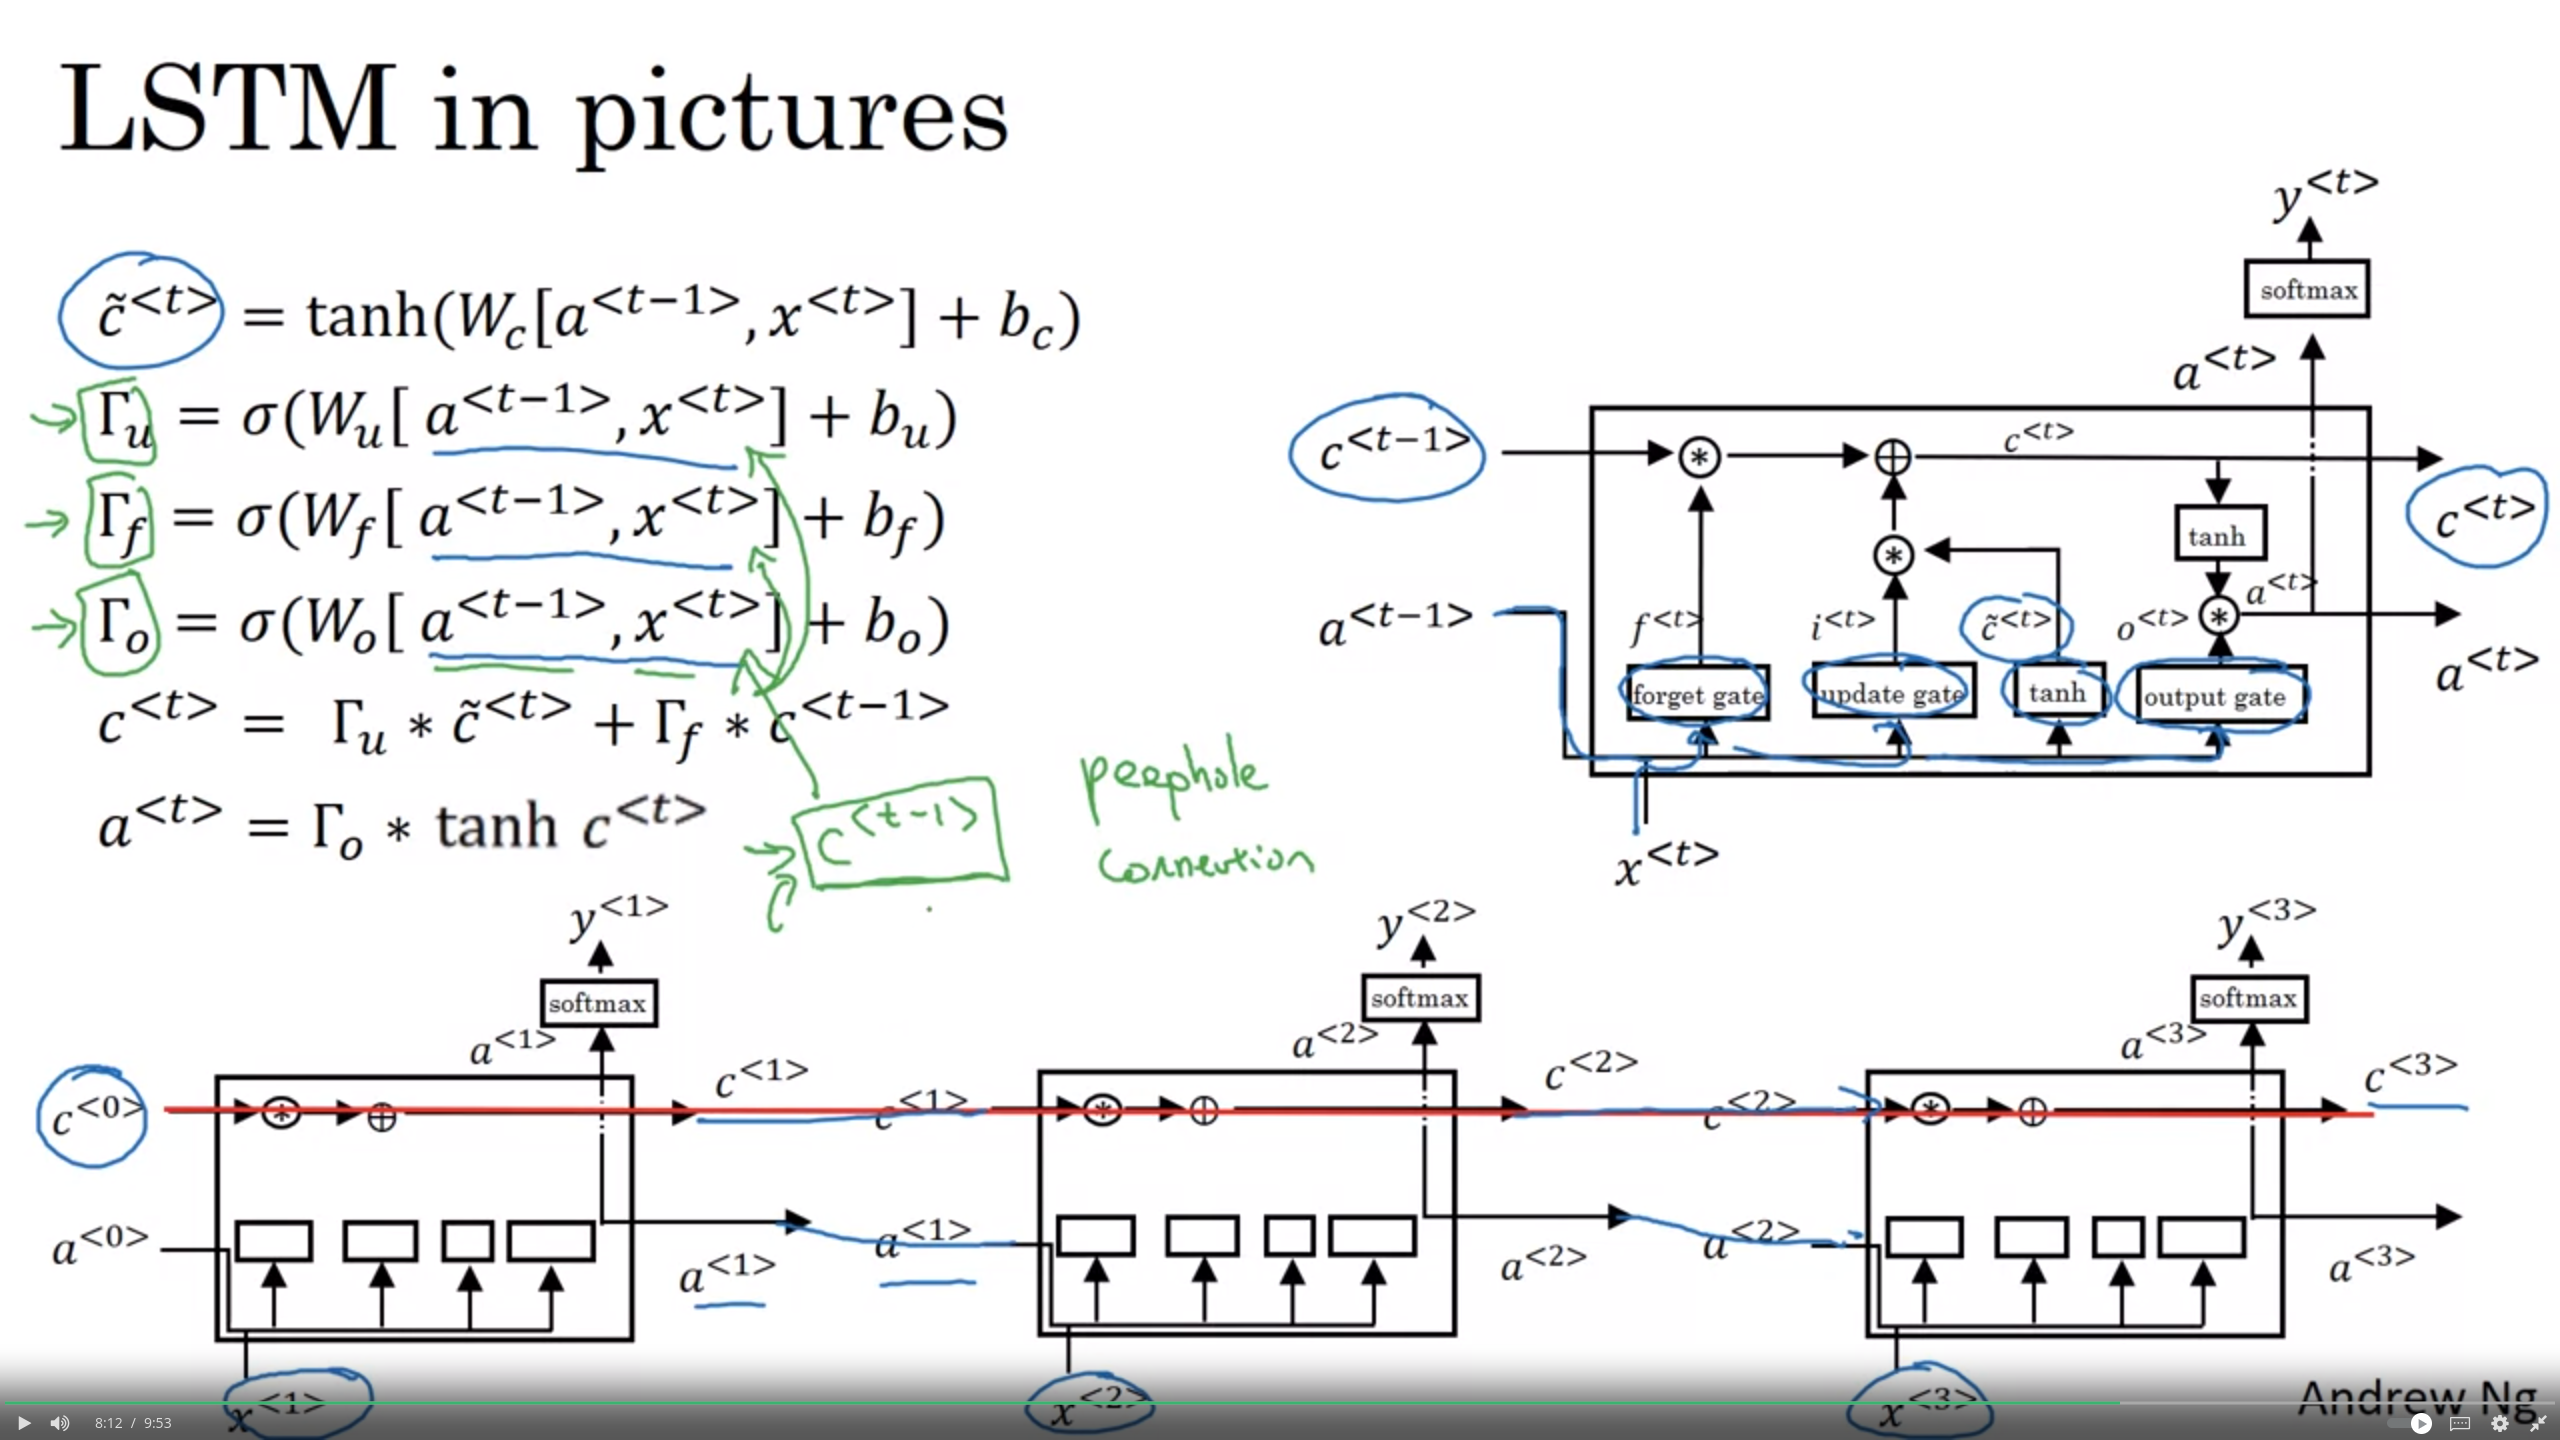
\includegraphics[trim =0.0cm 0.0cm 0.0cm 0.0cm, clip, scale=0.15]{pics/LSTM.png}
  \caption{LSTM}
  %{\footnotesize\textbf{Notes:} XXX.} % changed <<<<<<<<<<
  %#\label{XXX}
\end{figure}

Bidirectional RNN lets you at the point in time to take information from both earlier and later in the sequence.

Deep RNNs have hidden layers:
\begin{figure}[H]
  \centering
  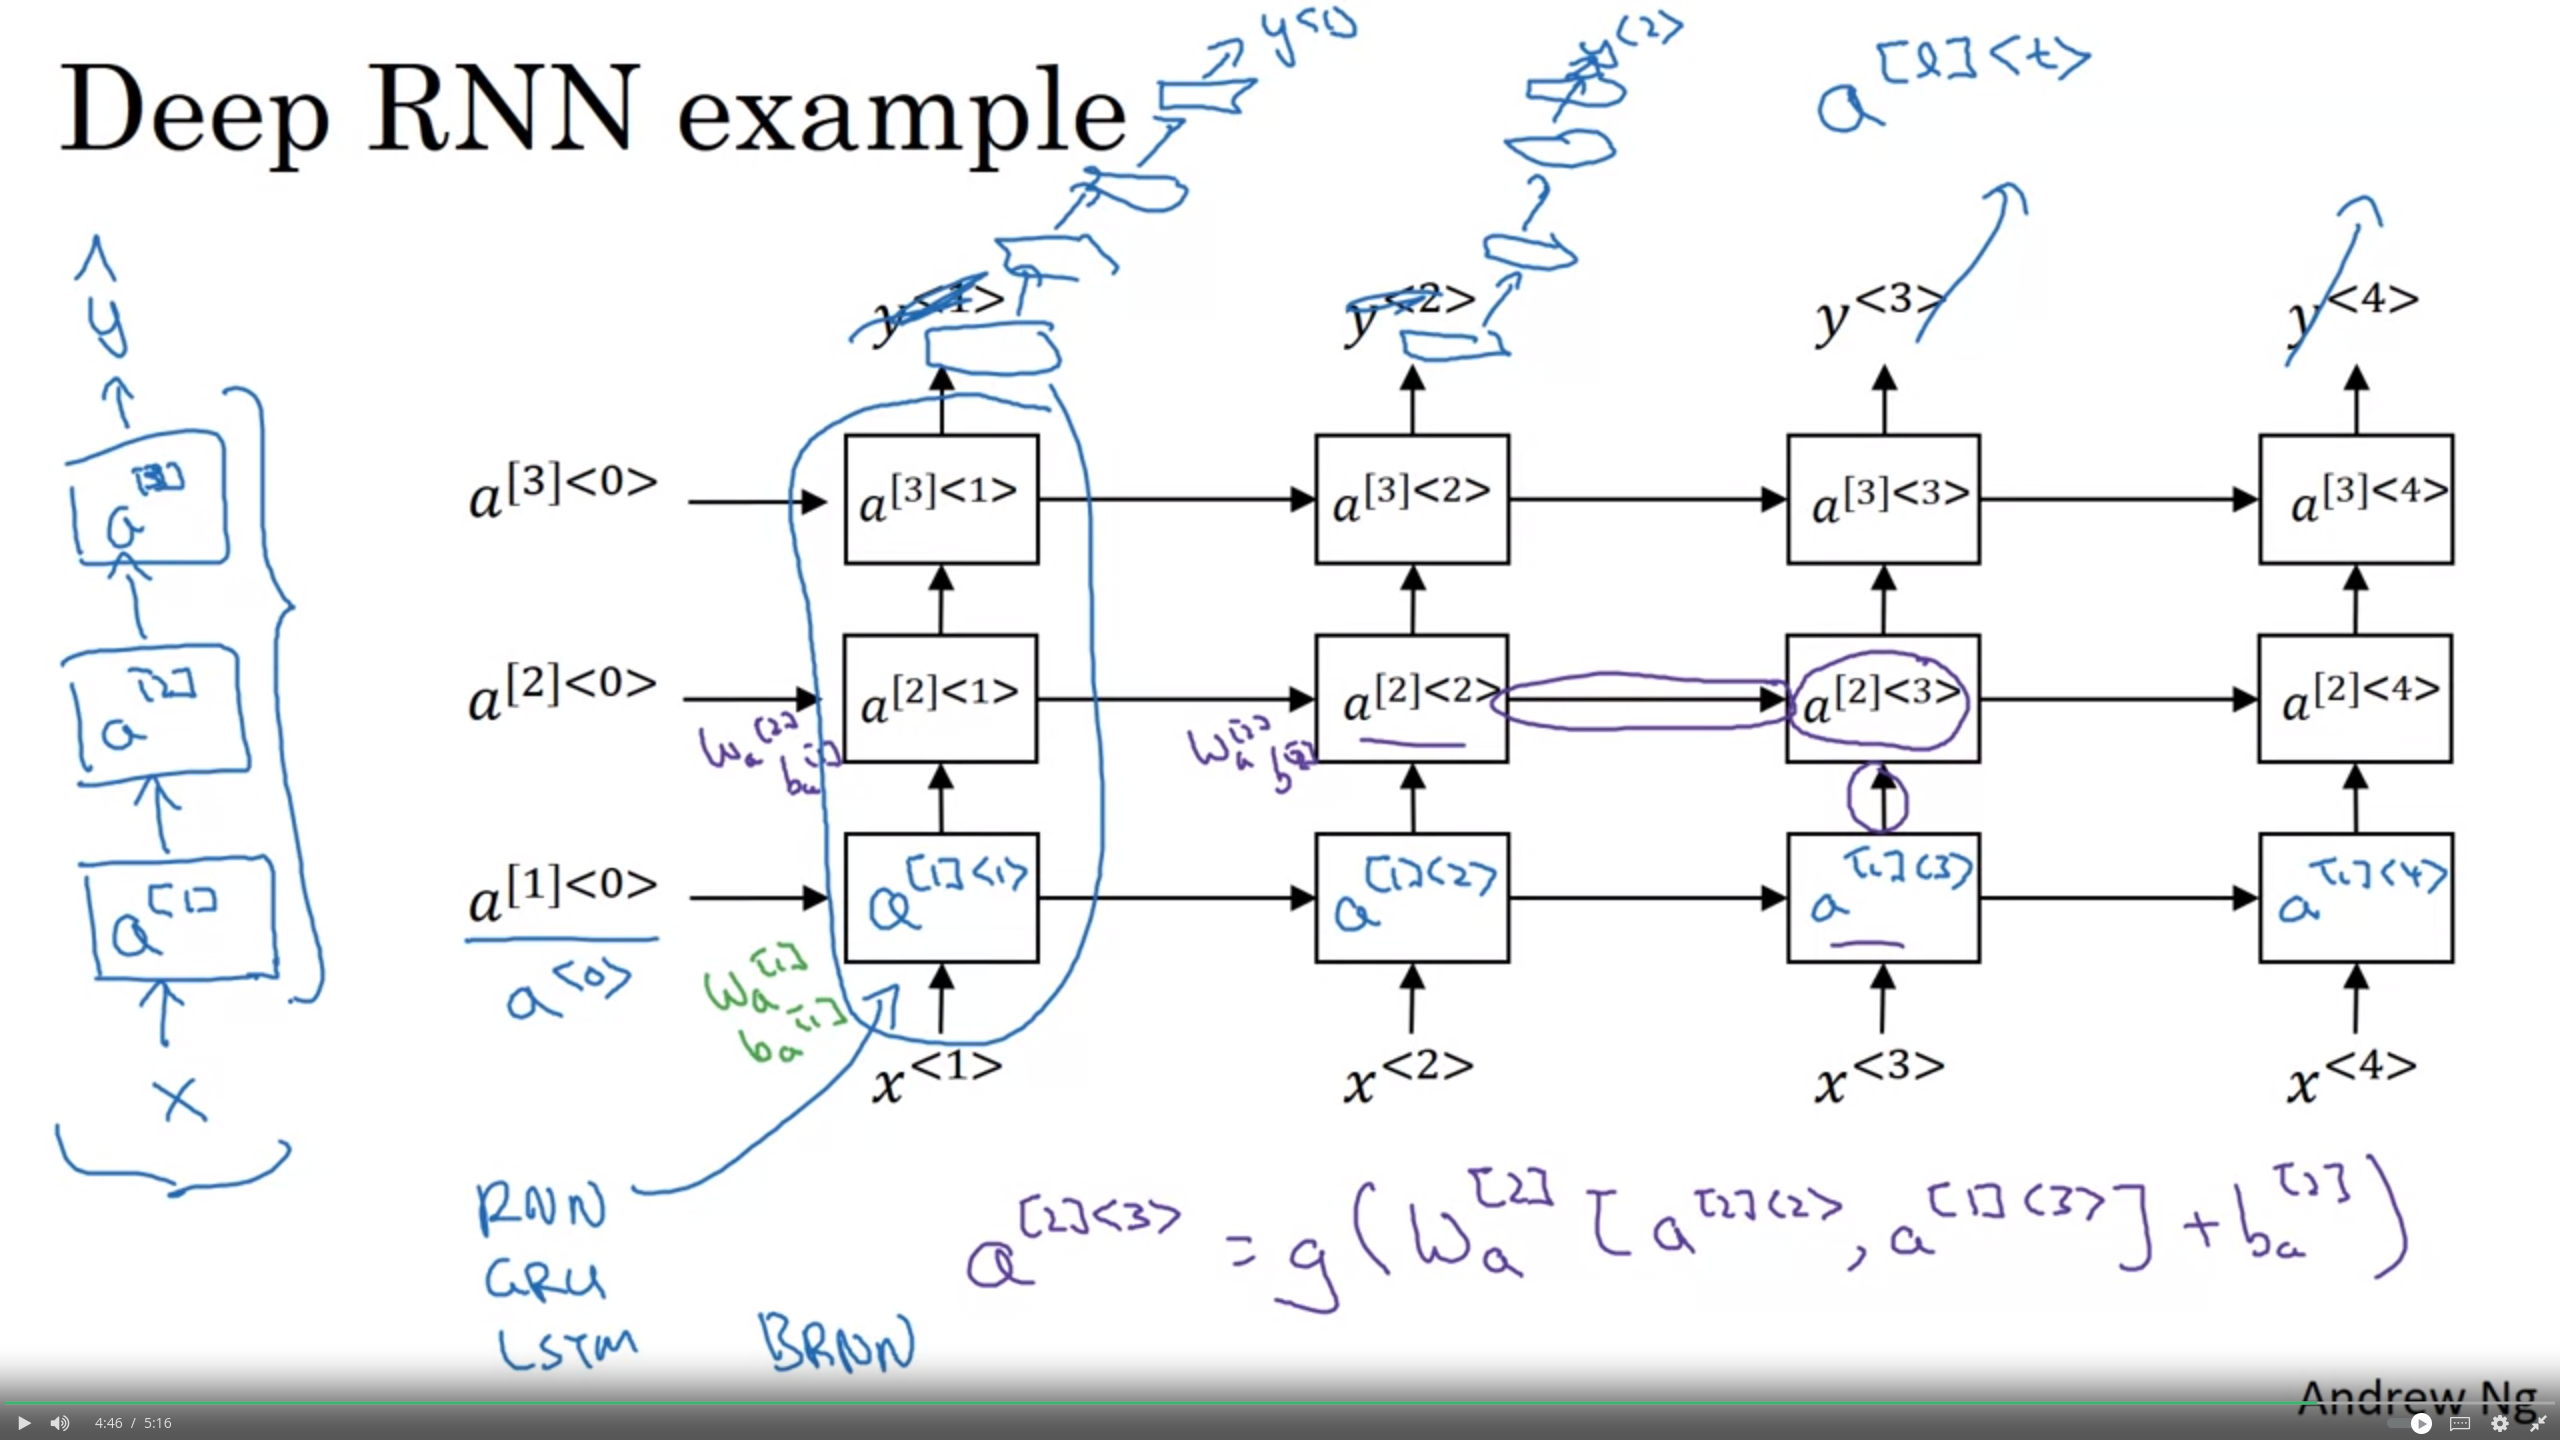
\includegraphics[trim =0.0cm 0.0cm 0.0cm 0.0cm, clip, scale=0.15]{pics/DRNN.png}
  \caption{LSTM}
  %{\footnotesize\textbf{Notes:} XXX.} % changed <<<<<<<<<<
  %#\label{XXX}
\end{figure}


\section{SL: Instance based learning}
\section{SL: Ensemble B\&B}

Ensemble Learning is in general the process of combining some simple rules into a more complex rule that can generalize well.

It works by dividing the data into smaller subsets, learn over each individual subset to come up with a rule, then combine all these rules in a single more complex rule. If we looked at the whole data, it would be hard to come up with simple rules.




\section{SL: Kernel methods and SVMs}
\section{SL: Comp Learning Theory}
\section{SL: VC dimensions}
\section{SL: Bayesian Learning}
\section{SL: Bayesian inference}


%===============================================================================
%===============================================================================
%===============================================================================
\chapter[Unsupervised learning]{Unsupervised learning (UL)}

Unsupervised algorithms don't make use of a target; instead, their purpose is to learn some property of the data, to represent the structure of the features in a certain way. In the context of feature engineering for prediction, you could think of an unsupervised algorithm as a "feature discovery" technique.

\section{Clustering}
Clustering simply means the assigning of data points to groups based upon how similar the points are to each other. When used for feature engineering, we could attempt to discover groups of customers representing a market segment, for instance, or geographic areas that share similar weather patterns. The other examples of using clustering is grouping similar news, DNA analysis, astronomical data analysis.


The motivating idea for adding cluster labels is that the clusters will break up complicated relationships across features into simpler chunks. Our model can then just learn the simpler chunks one-by-one instead having to learn the complicated whole all at once. It's a "divide and conquer" strategy.

There are \href{https://www.geeksforgeeks.org/different-types-clustering-algorithm/#}{multiple methods} for clustering. They differ primarily in how they measure \textit{similarity} or \textit{proximity} and in what kinds of features they work with. Clustering algorithms include: Distribution-based methods (expectation-maximization algorithm), Centroid-based methods (K-means), Connectivity-based methods (hierarchical algorithms), Density model (DBSCAN), and subspace clustering.

\subsection{K-means clustering}
It measures similarity using ordinary straight-line distance (Euclidean distance). It creates clusters by placing a number of points, called centroids, inside the feature-space. Each point in the dataset is assigned to the cluster of whichever centroid it's closest to. The "k" in "k-means" is how many centroids it creates.

Clustering has two main steps, selecting or moving centriods, and then assigning nodes to centriods. To do the clustering, we randomly select k points/centroids in the space, not necessarily a real point from the data set, but just in the space3. Then, it calculates the distance between each node and the centroids, and assigns each node to closest centriod. For the next iteration, we need to adjust the centriod. First, we find the average of each cluster points, and use that one as the new centriod. We repeat the process, until the point is not moving. In the first step, we keep the centriods fixed and just change the point assignments. In the next step, centriods change. This method is guaranteed to converge.

\begin{figure}[H]
  \centering
  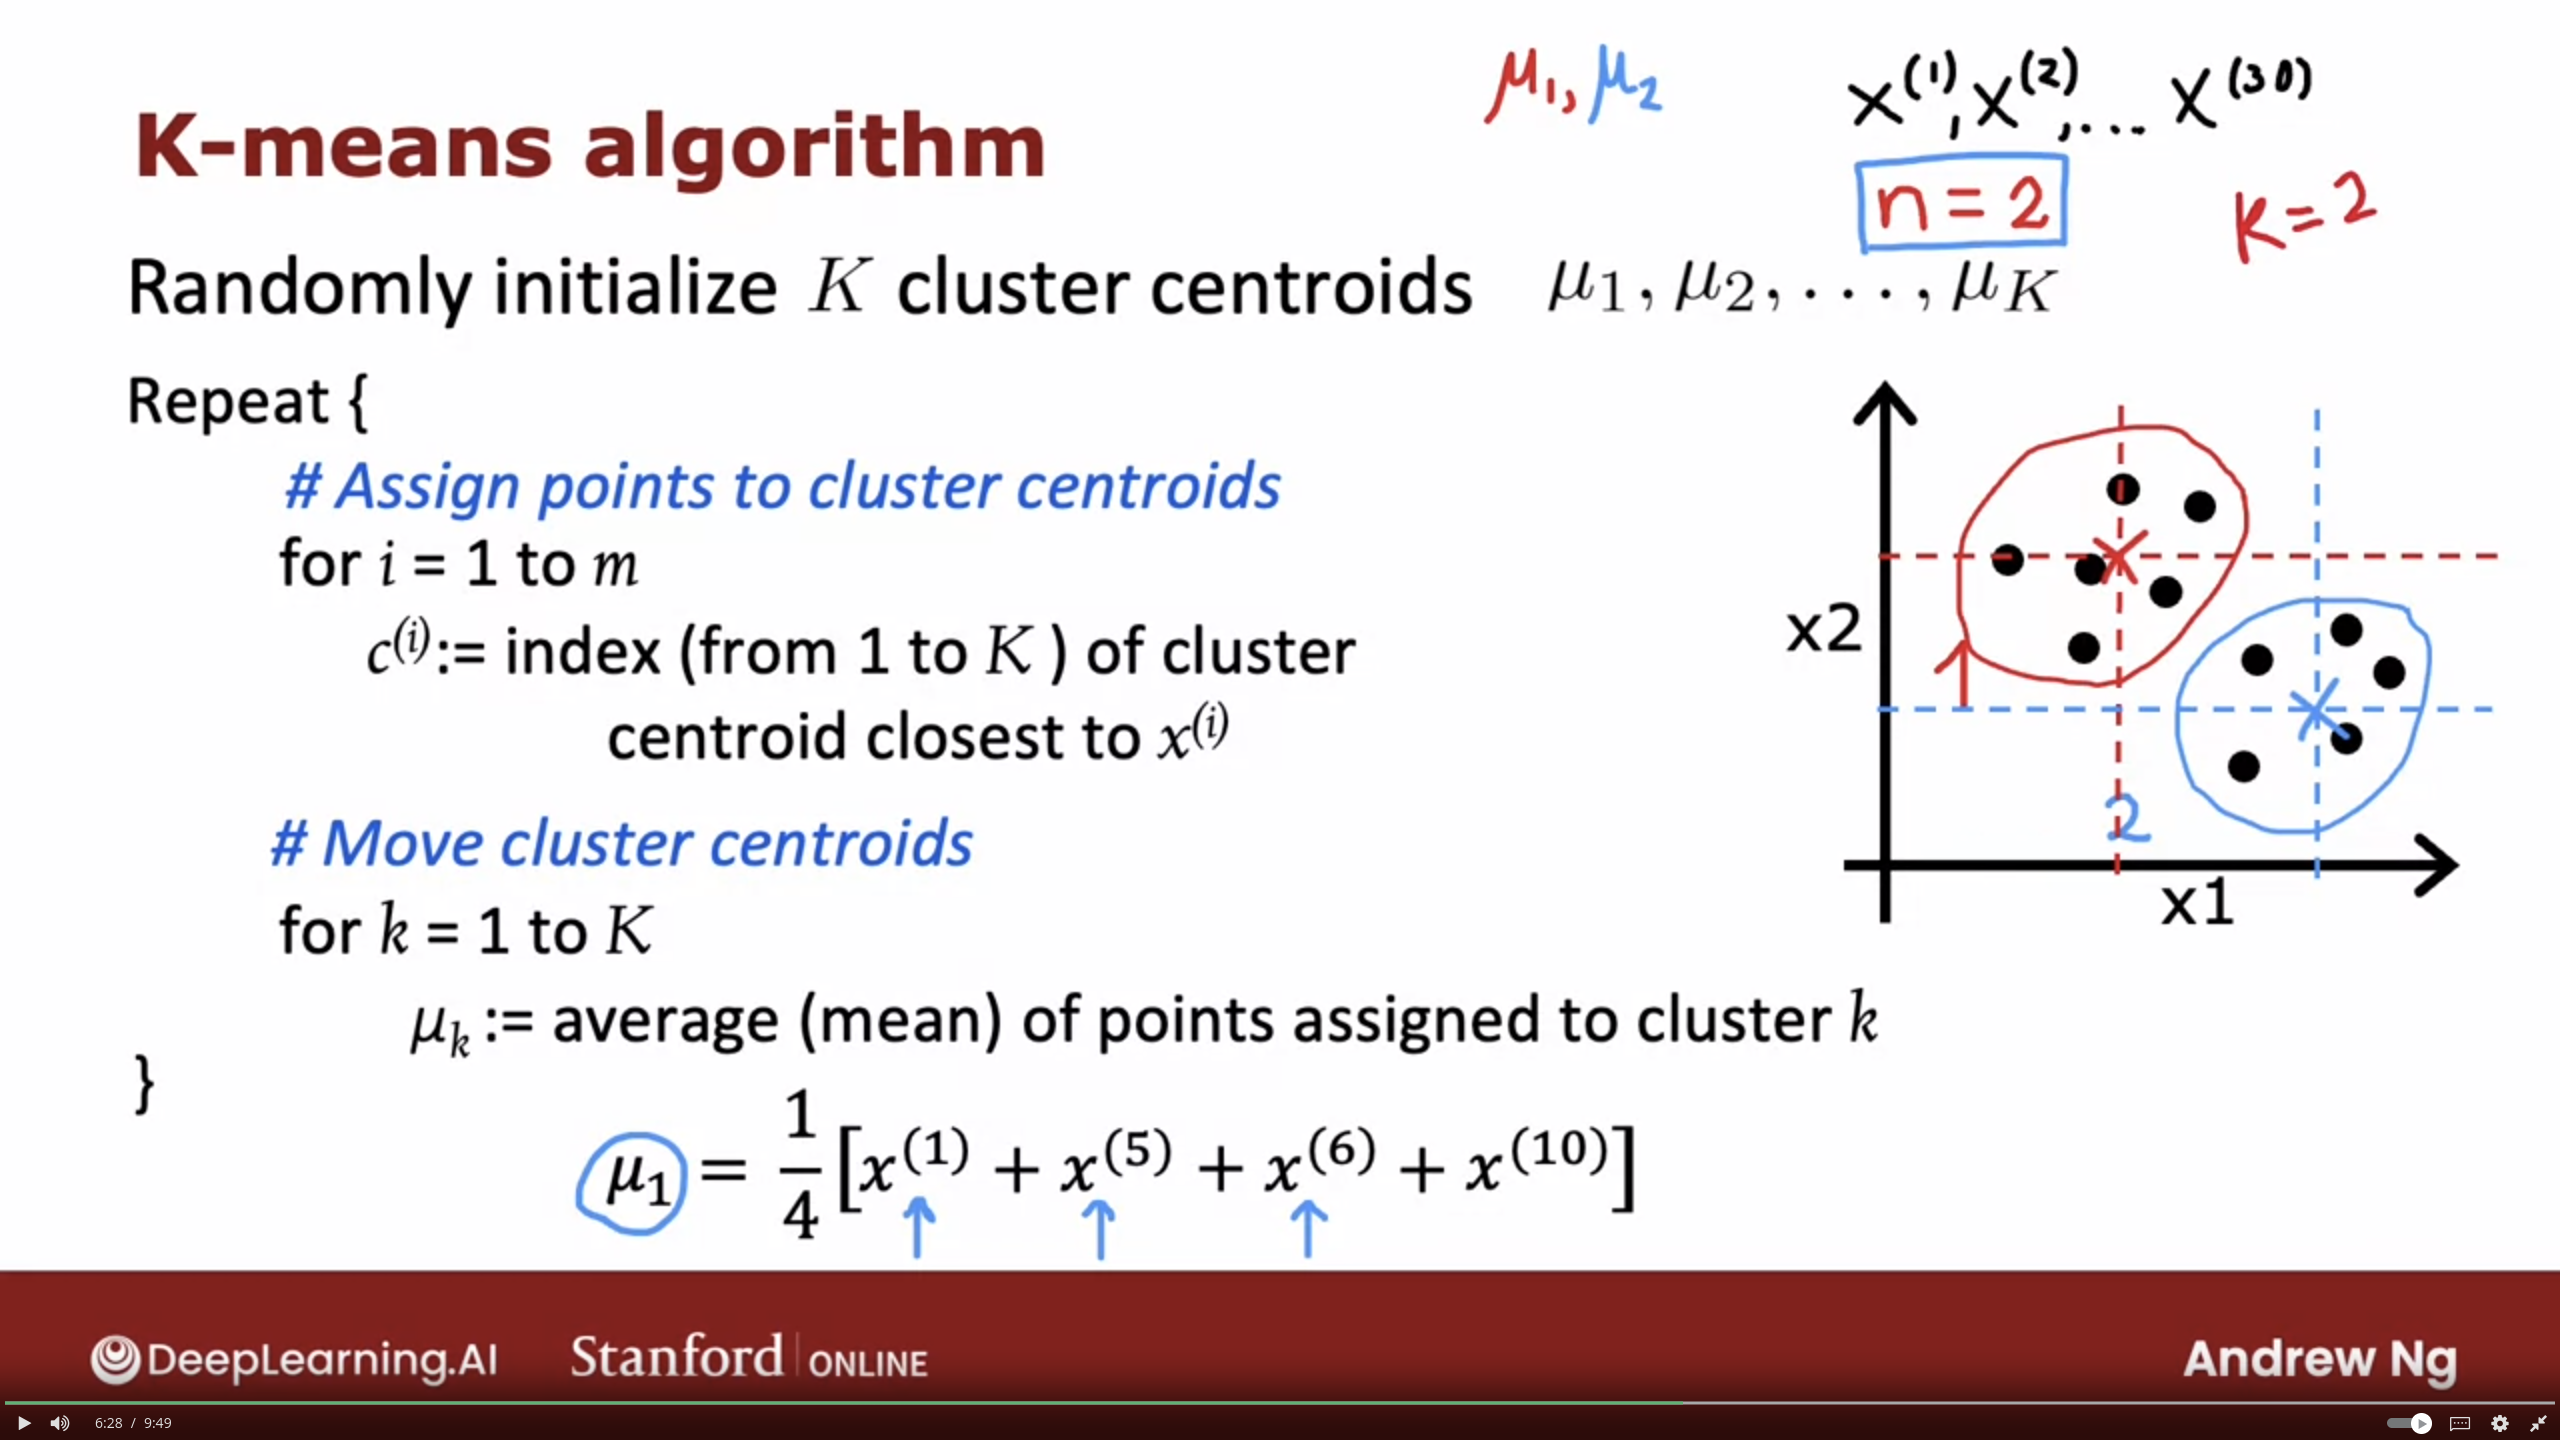
\includegraphics[trim =0.0cm 0.0cm 0.0cm 0.0cm, clip, scale=0.15]{pics/cluster.png}
  \caption{K-mean clustering}
  %{\footnotesize\textbf{Notes:} XXX.} % changed <<<<<<<<<<
  %#\label{XXX}
\end{figure}


The only exception is that if there is no point assigned to a centriod, which means calculating the average is not defined. In that case, we either eliminate the cluster point, or randomly assign a new point to the cluster. Sometimes, the points are not really separated/clustered. In that case, theoretically, it is more difficult to decide how many points are needed.


The K-mean algorithm is indeed an optimization problem, based on the distortion cost function.

\begin{figure}[H]
  \centering
  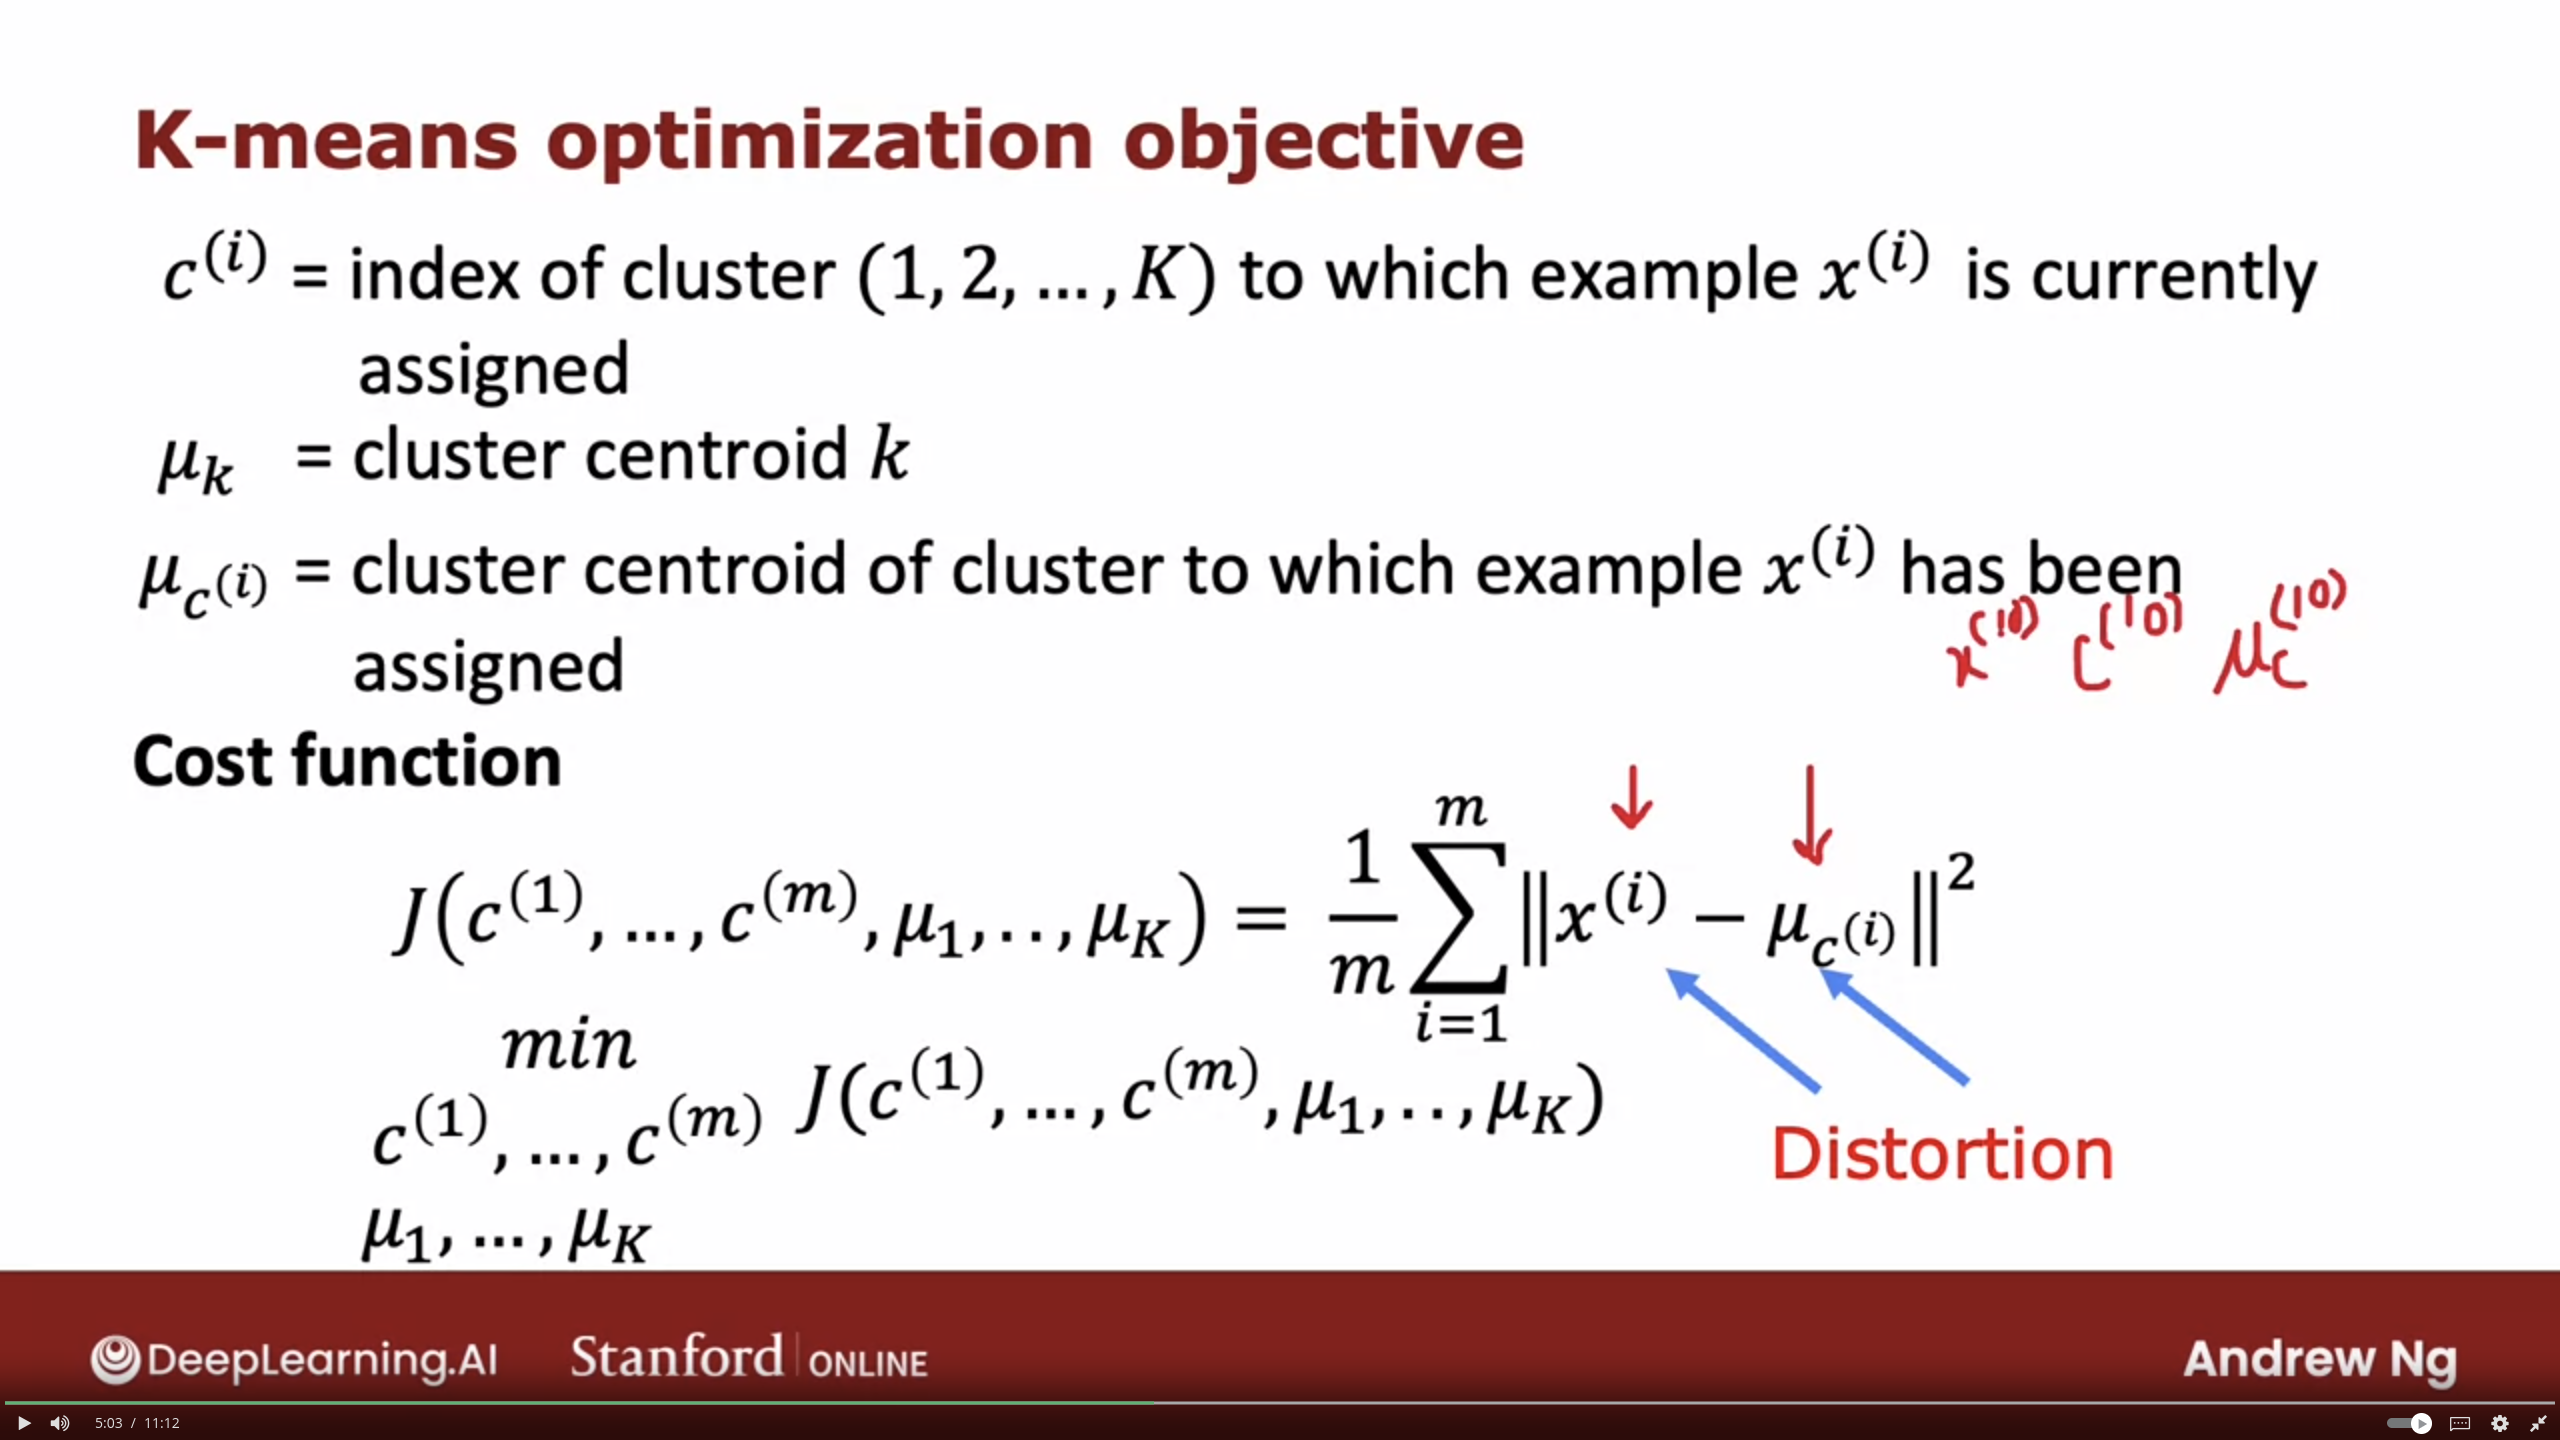
\includegraphics[trim =0.0cm 0.0cm 0.0cm 0.0cm, clip, scale=0.15]{pics/distortion.png}
  \caption{K-mean clustering distortion optimizer}
  %#\label{XXX}
\end{figure}




The very first step of the K-means algorithm is the initial guess for the number of clusters and the location of centriods. K should definitely be less than the number of points. To find out the best K for a data set, we can test various K numbers and plot K vs variance, this is called an \textit{elbow plot}. The best K is the one that the slope of variance reduces. If K is equal to the number of items in the dataset, then, the variance would be zero. The other factor is that how you want to use the clusters, the larger the K is, may cause a higher cost.

\begin{figure}[H]
  \centering
  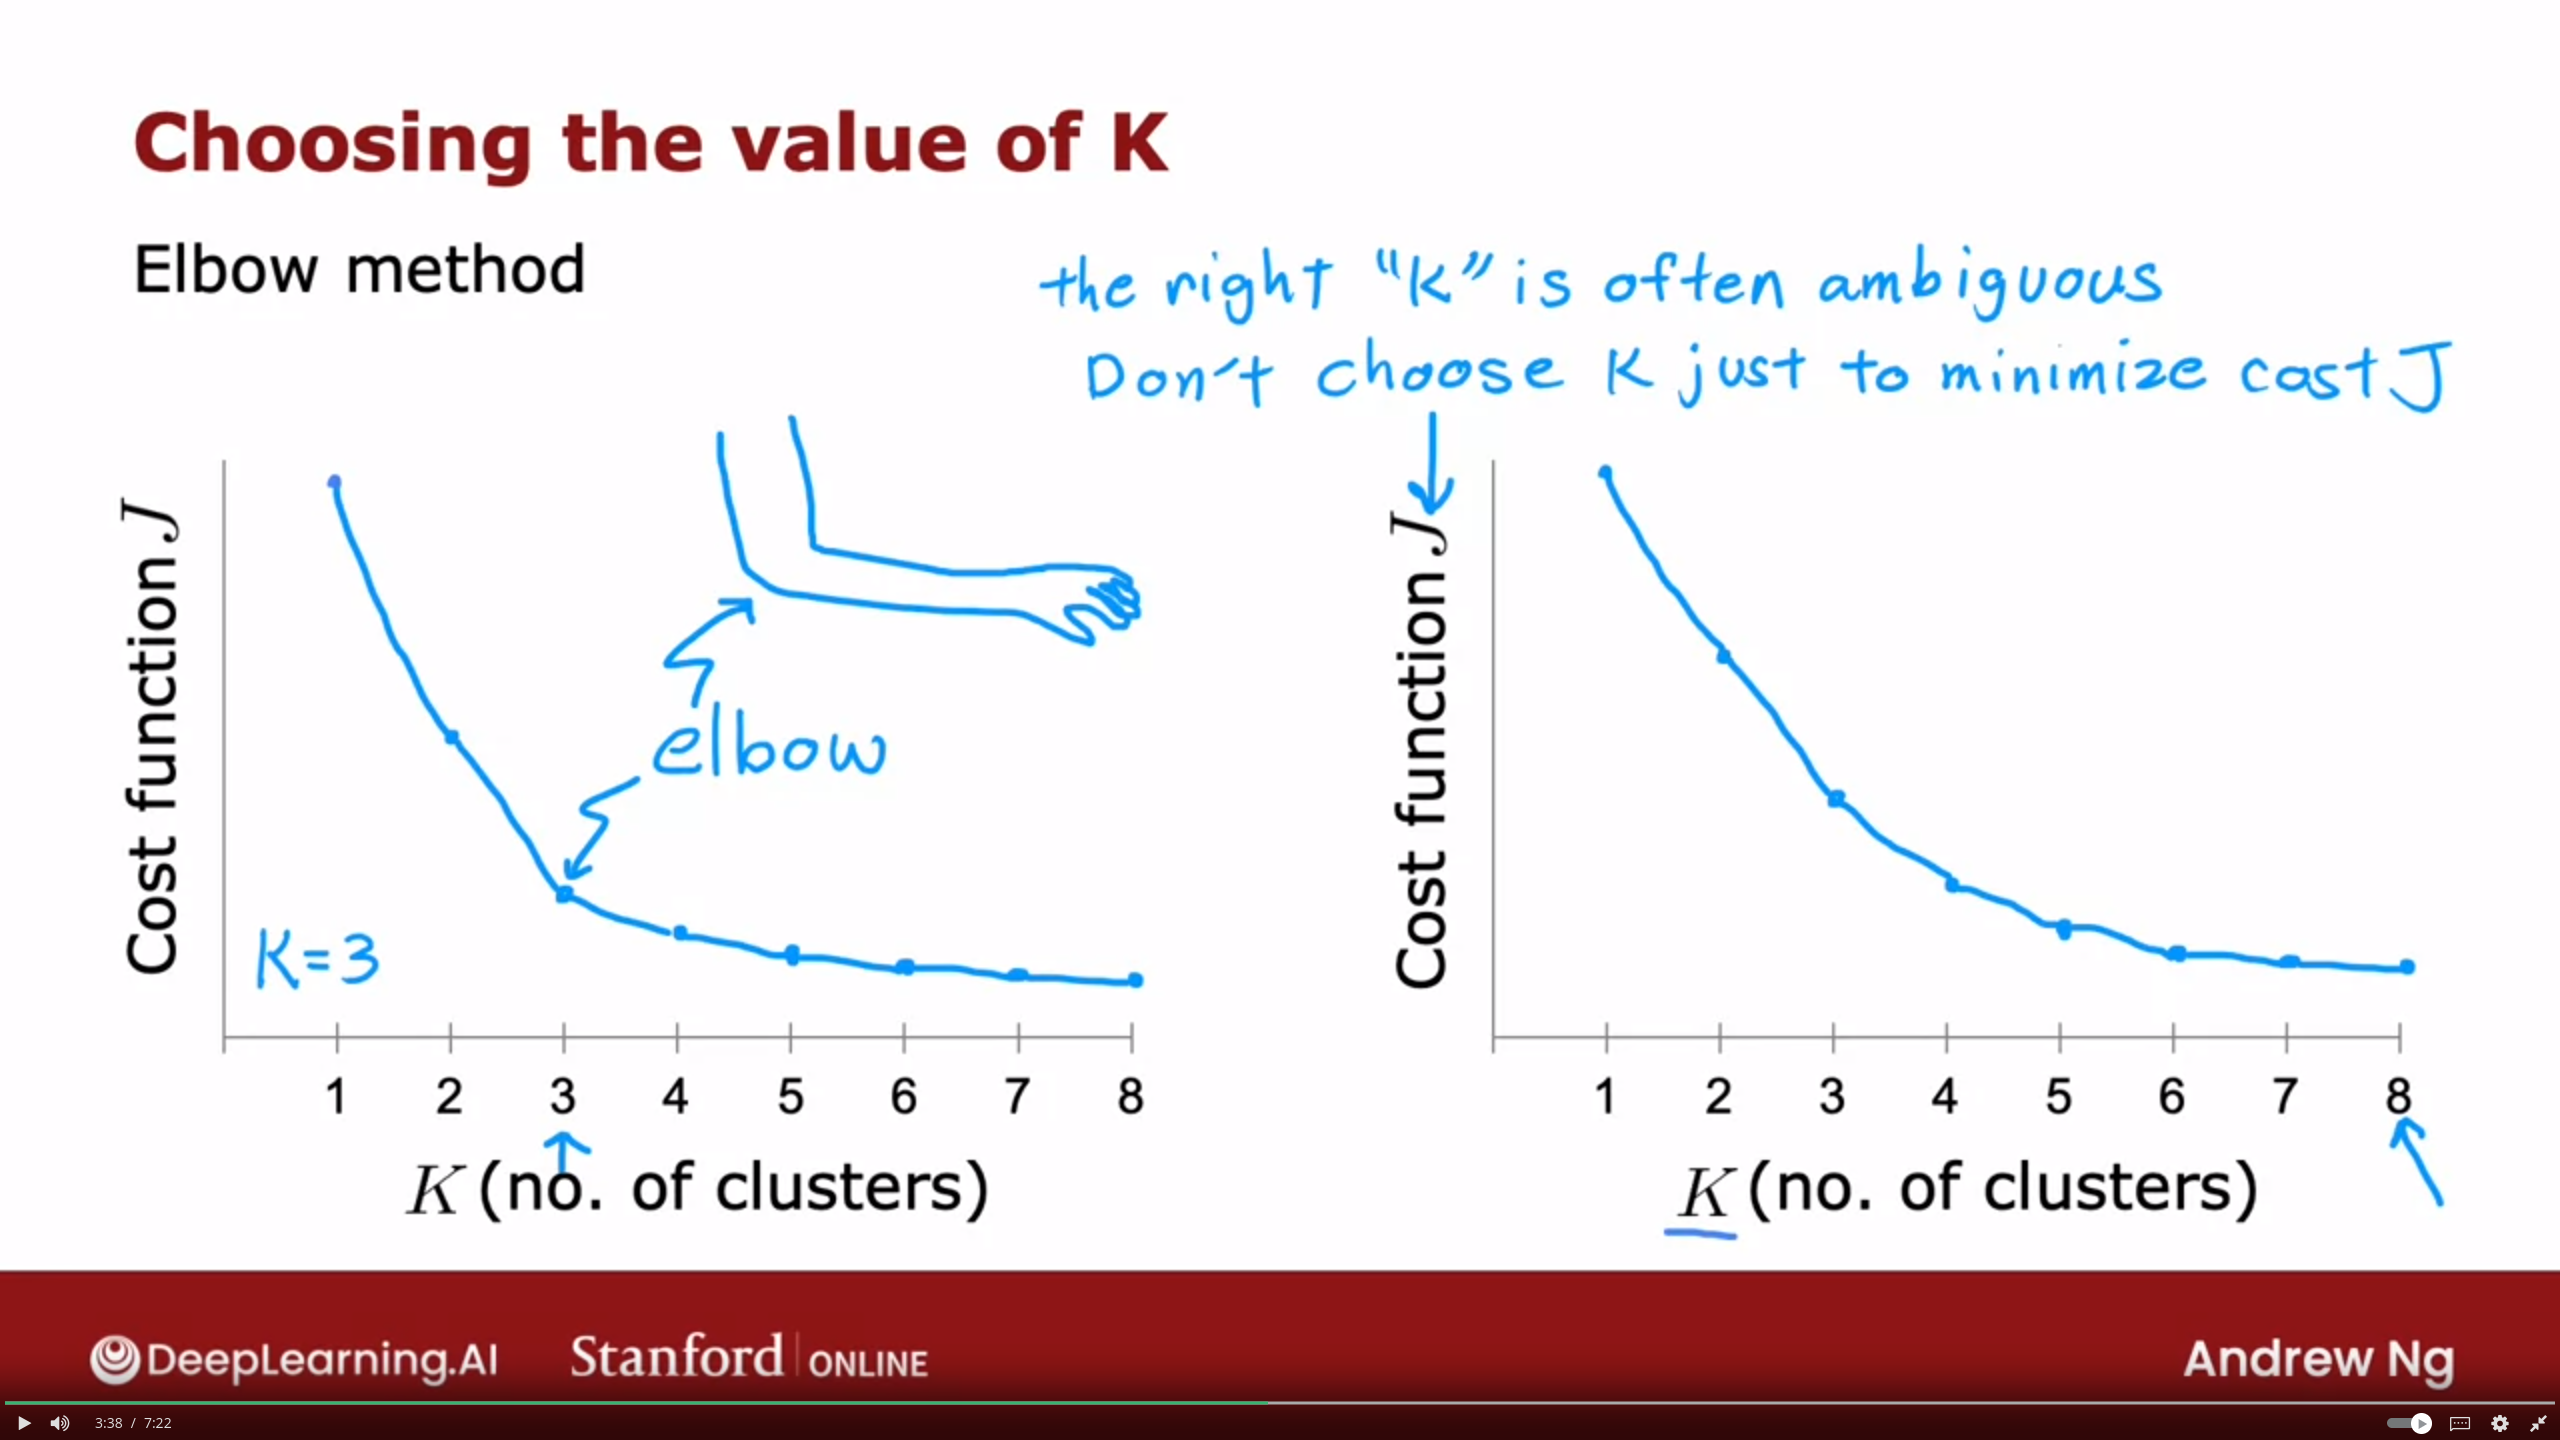
\includegraphics[trim =0.0cm 0.0cm 0.0cm 0.0cm, clip, scale=0.15]{pics/elbow.png}
  \caption{K-mean clustering, K selection}
  %{\footnotesize\textbf{Notes:} XXX.} % changed <<<<<<<<<<
  %#\label{XXX}
\end{figure}



For the location of centriods, we can randomly choose from nodes. The downside of this method is that we may stuck in the local minimum. To avoid that, we can run this process multiple times and select the one with the lowest cost.


\begin{figure}[H]
  \centering
  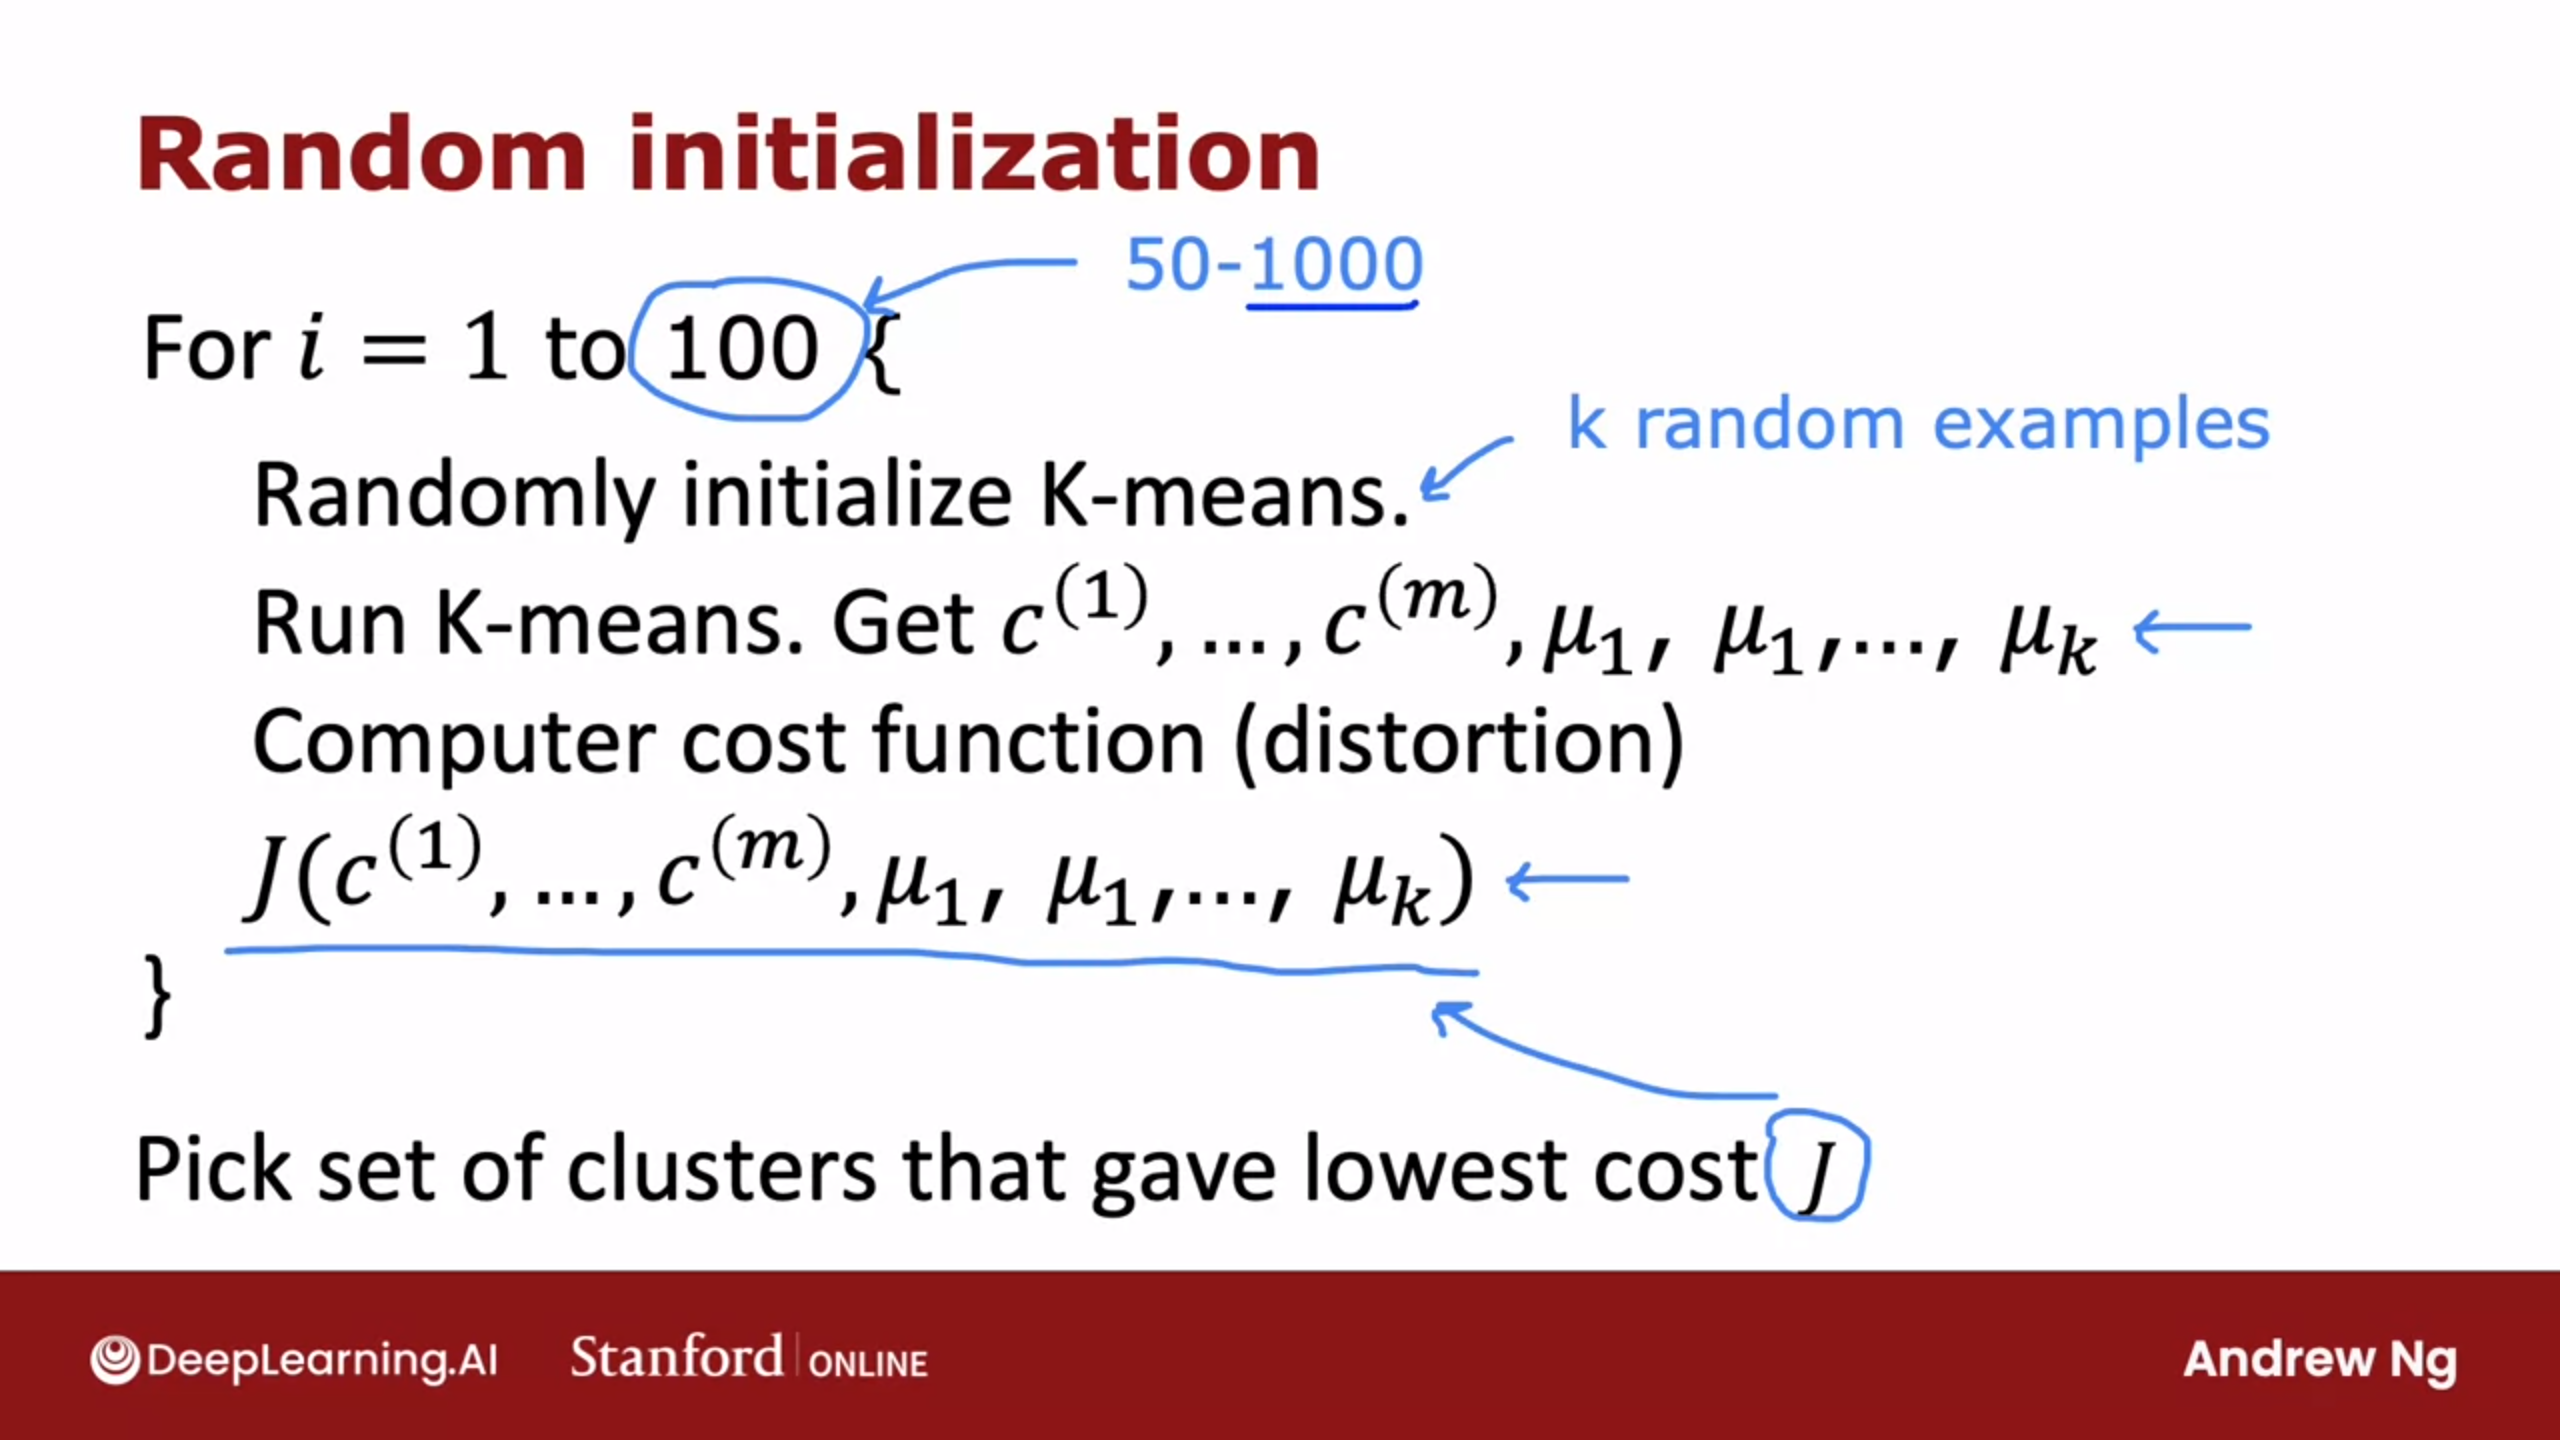
\includegraphics[trim =0.0cm 0.0cm 0.0cm 0.0cm, clip, scale=0.15]{pics/k-initialization.png}
  \caption{K-mean clustering initialization}
  %{\footnotesize\textbf{Notes:} XXX.} % changed <<<<<<<<<<
  %#\label{XXX}
\end{figure}


The k-means algorithm is sensitive to scale. This means we need to be thoughtful about how and whether we rescale our features since we might get very different results depending on our choices. As a rule of thumb, if the features are already directly comparable (like a test result at different times), then you would *not* want to rescale. On the other hand, features that aren't on comparable scales (like height and weight) will usually benefit from rescaling. Sometimes, the choice won't be clear though. In that case, you should try to use common sense, remembering that features with larger values will be weighted more heavily.

What you should take away from this is that the decision of whether and how to rescale features is rarely automatic -- it will usually depend on some domain knowledge about your data and what you're trying to predict. Comparing different rescaling schemes through cross-validation can also be helpful.




\subsection{Principal Component Analysis (PCA)}
Just like clustering is a partitioning of the dataset based on proximity, you could think of PCA as a partitioning of the variation in the data. PCA is a great tool to help you discover important relationships in the data and can also be used to create more informative features. PCA is typically applied to standardized data. With standardized data "variation" means "correlation". With unstandardized data "variation" means "covariance". All data in this course will be standardized before applying PCA. The main idea of PCA: instead of describing the data with the original features, we describe it with its axes of variation. The axes of variation become the new features. The new features PCA constructs are actually just linear combinations (weighted sums) of the original features. These new features are called the principal components of the data. The weights themselves are called loadings.

PCA also tells us the amount of variation in each component. We can see from the figures that there is more variation in the data along the Size component than along the Shape component. PCA makes this precise through each component's percent of explained variance. It's important to remember, however, that the amount of variance in a component doesn't necessarily correspond to how good it is as a predictor: it depends on what you're trying to predict.


\section{Anomaly detection}
The idea is to build and train a (unsupervised) model based on some samples and their features, then the task for this model is to review any new sample and find out if there is any anomaly with the features. The method for this task is called density estimation. In this method, we find regions with different levels of probability/anomaly, in which, if the new sample features locate in the high probability area, there is no anomaly, but as we move away from it, anomaly probability increases. This method has several applications including fraud detection, manufacturing, monitoring computers in data centers, etc.

\begin{figure}[H]
  \centering
  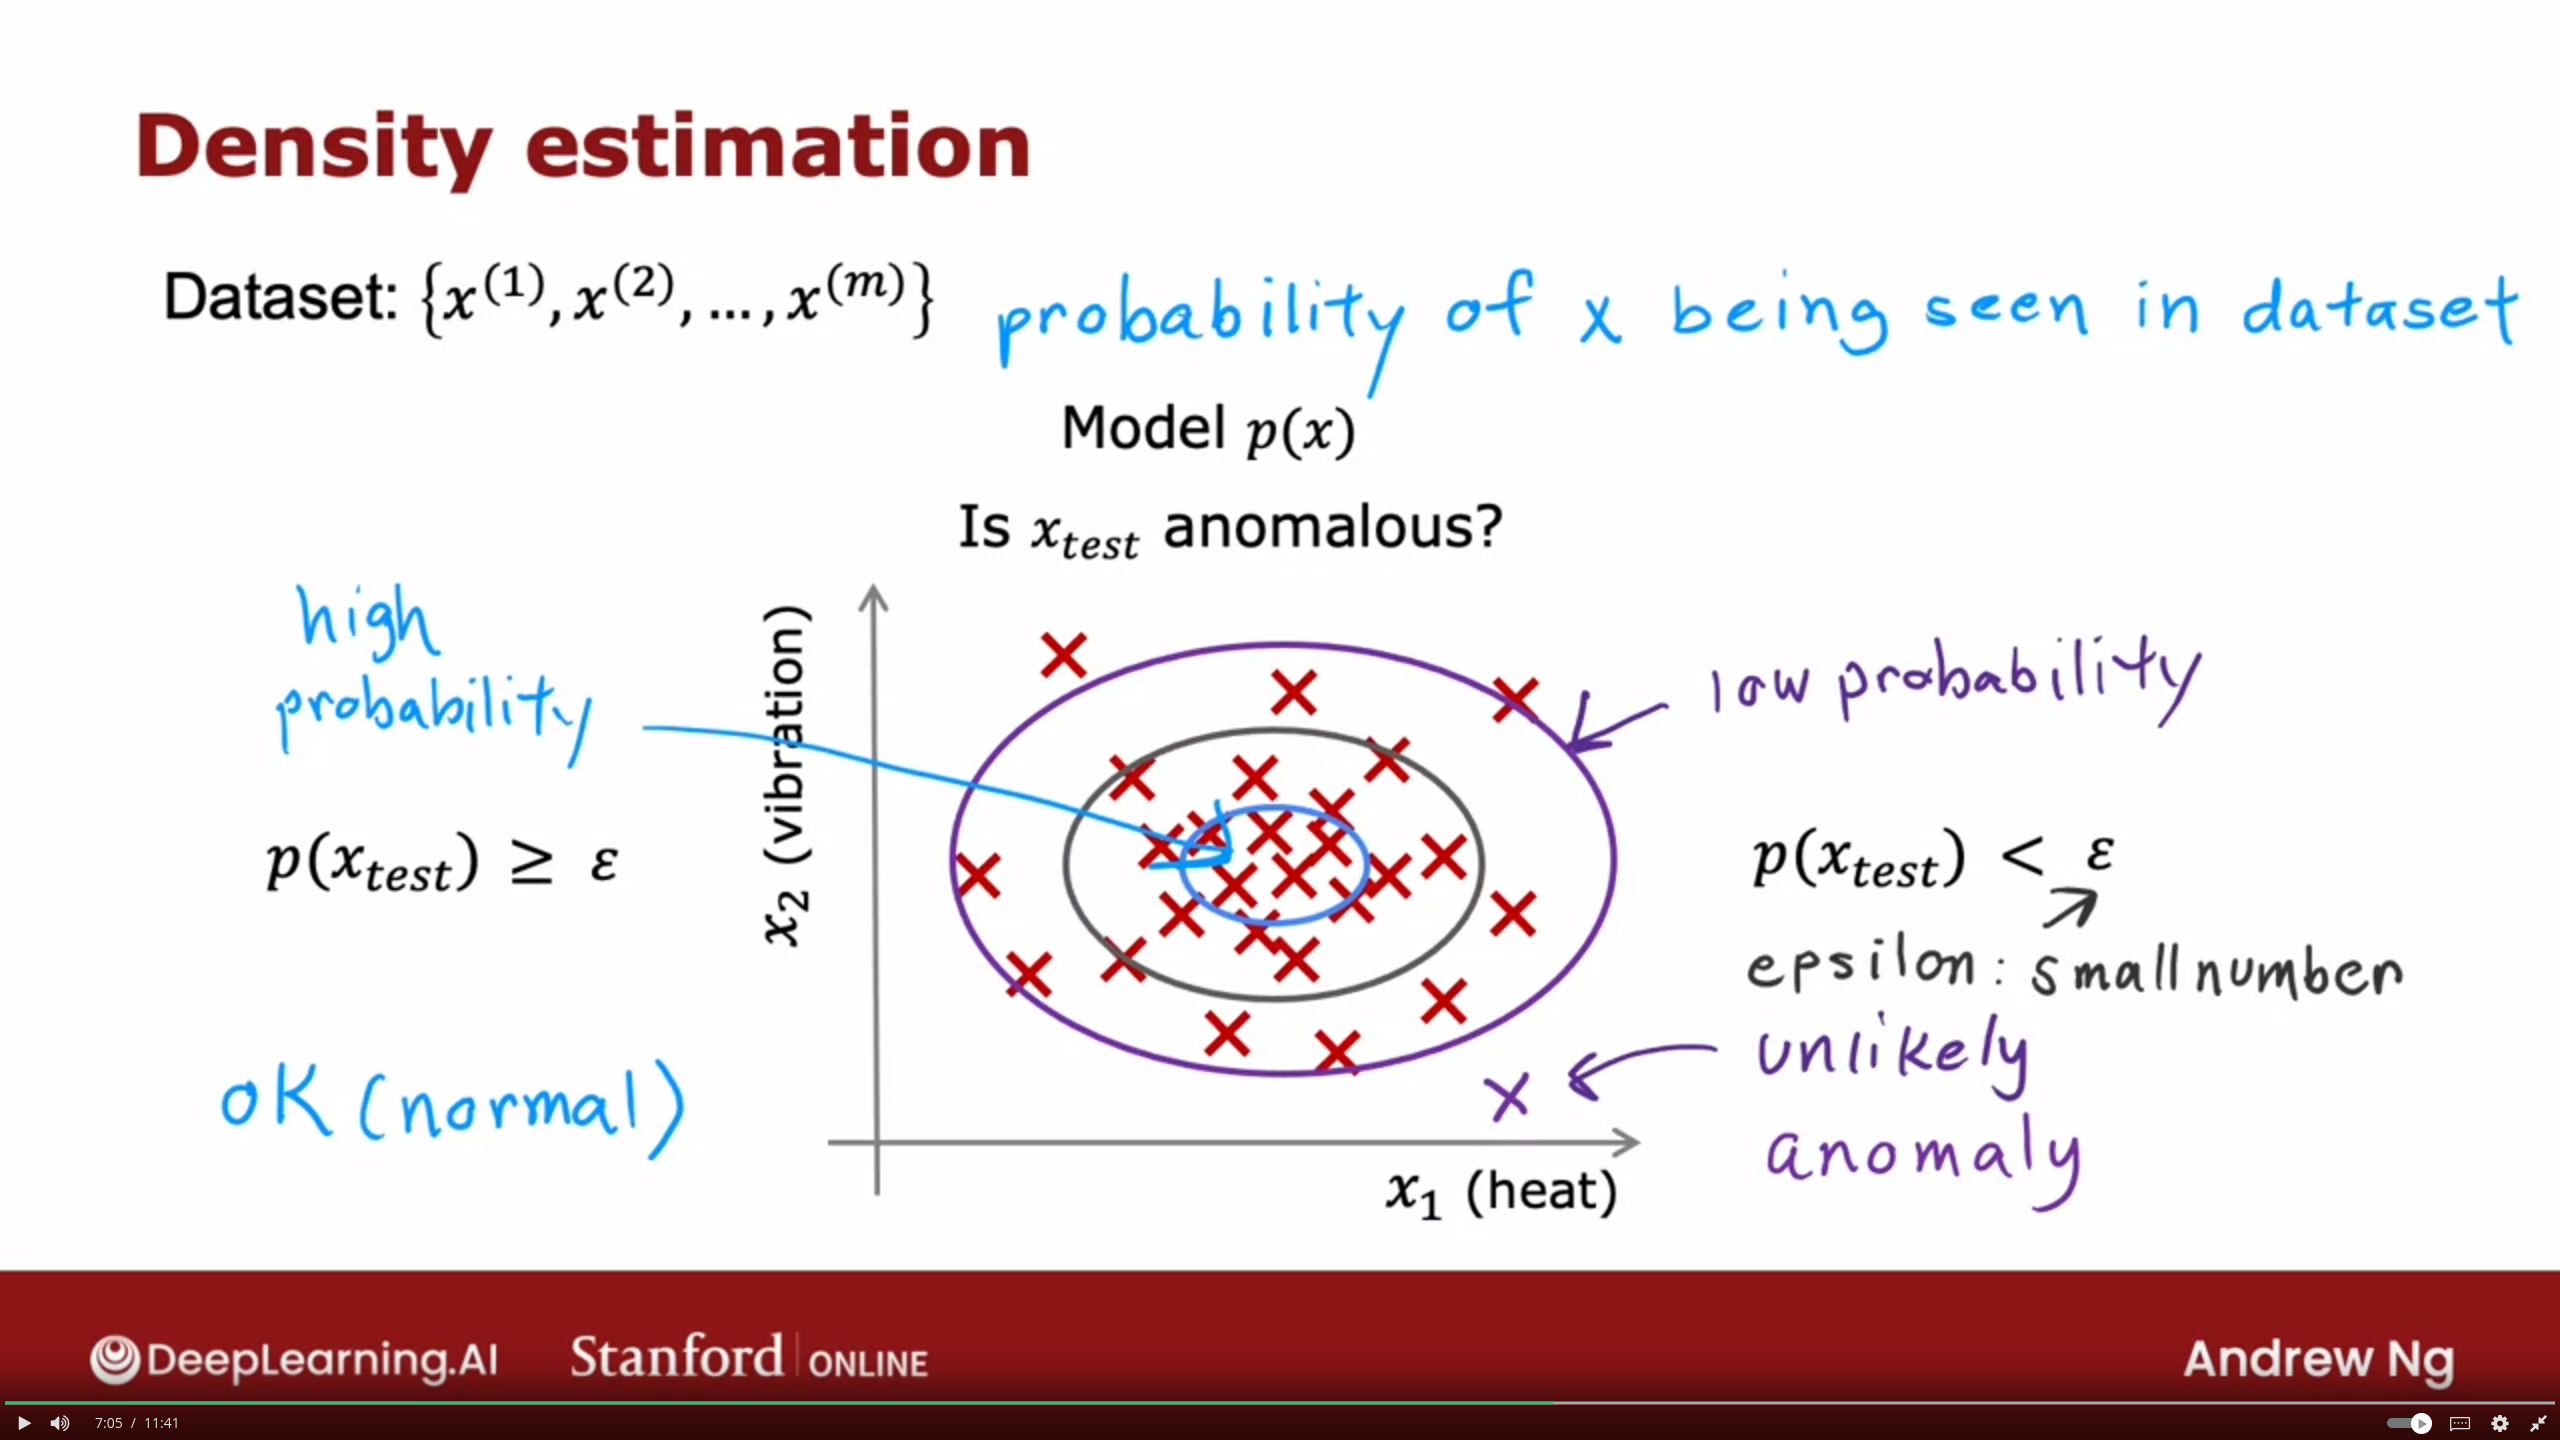
\includegraphics[trim =0.0cm 0.0cm 0.0cm 0.0cm, clip, scale=0.15]{pics/density.png}
  \caption{Density estimation}
  %{\footnotesize\textbf{Notes:} XXX.} % changed <<<<<<<<<<
  %#\label{XXX}
\end{figure}

To apply anomaly detection, we use Gaussian (normal/bell shape) distribution. The next picture shows the distribution equation:

\begin{figure}[H]
  \centering
  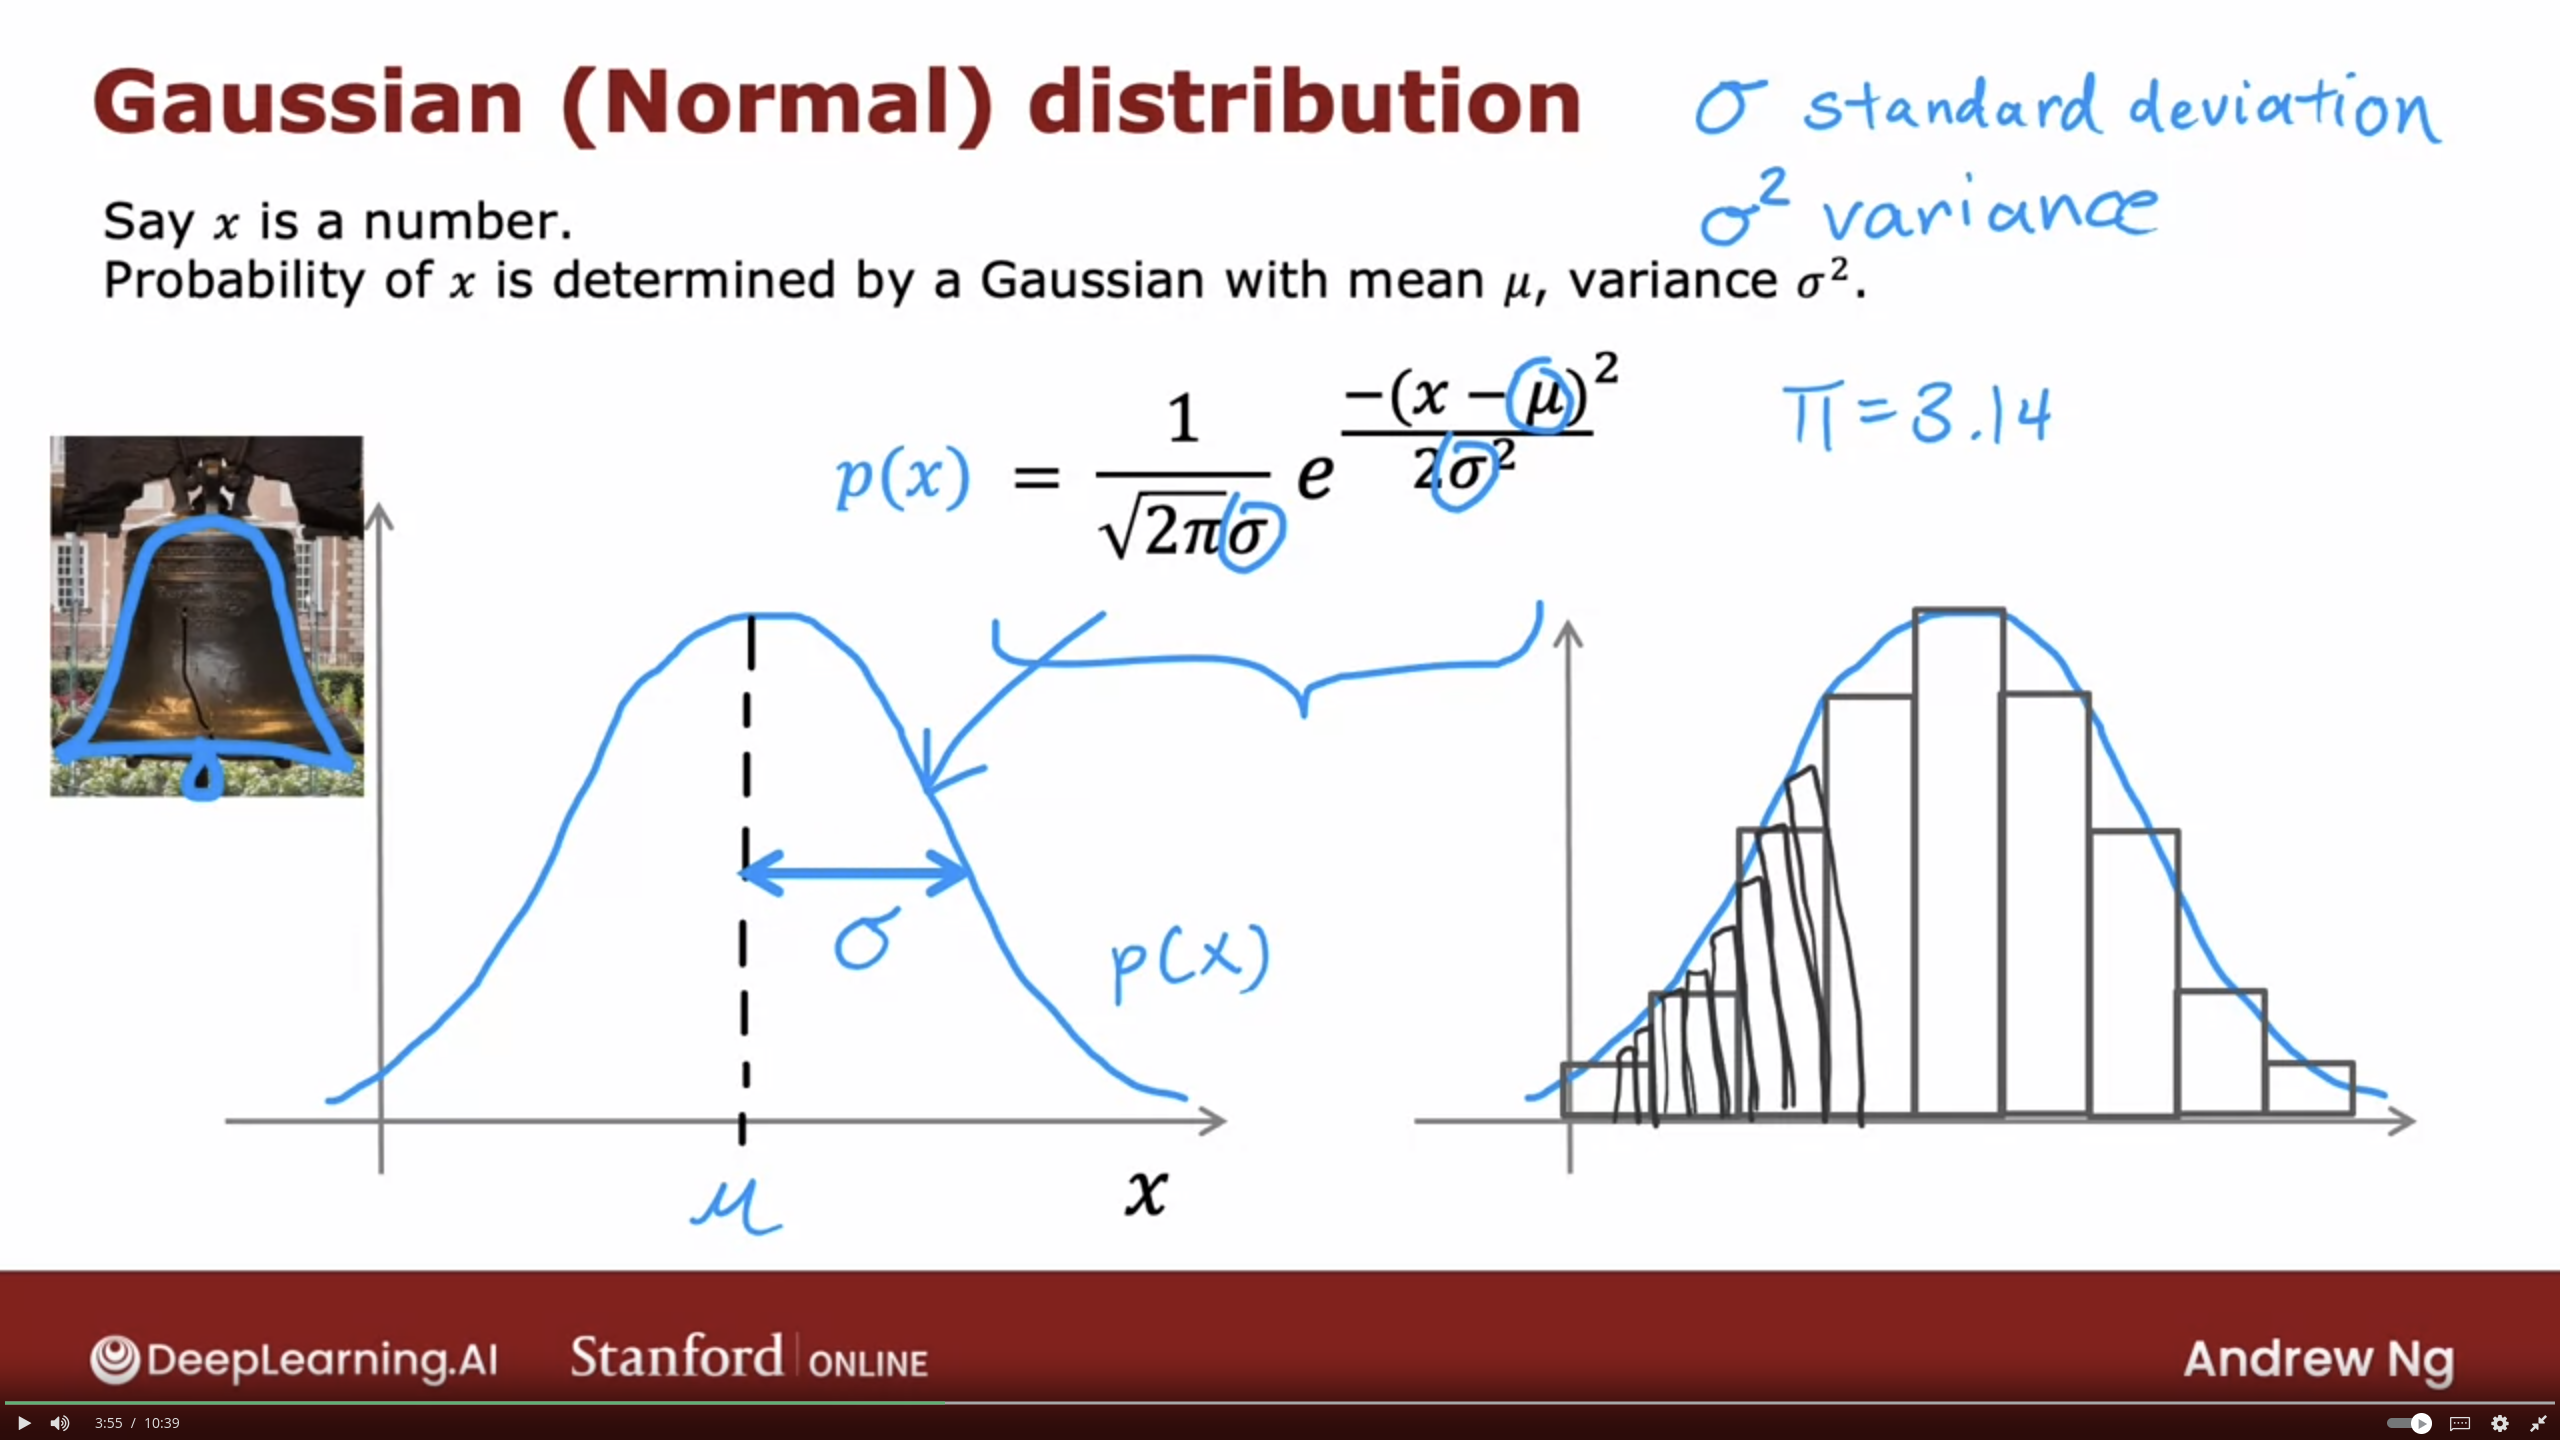
\includegraphics[trim =0.0cm 0.0cm 0.0cm 0.0cm, clip, scale=0.15]{pics/gaussian.png}
  \caption{Gaussian distribution}
  %{\footnotesize\textbf{Notes:} XXX.} % changed <<<<<<<<<<
  %#\label{XXX}
\end{figure}

To calculate the Gaussian distribution for a set of data:

\begin{equation}
  \mu = \frac{1}{m} \Sigma_{i=1}^{m} x ^ {(i)} \newline
  \sigma^2 = \frac{1}{m} \Sigma_{i=1}^{m} \big(x ^ {(i)} -\mu  \big)^2
\end{equation}
but notice that each sample might have multiple features. To calculate the probability of one sample, then we need to multiply the probability of each each feature. Multiplication is only valid if the features are statically independent, which is usually not the case, but for this purpose, it is fine to use multiplication, even though features are dependent. Here is how it works:

\begin{figure}[H]
  \centering
  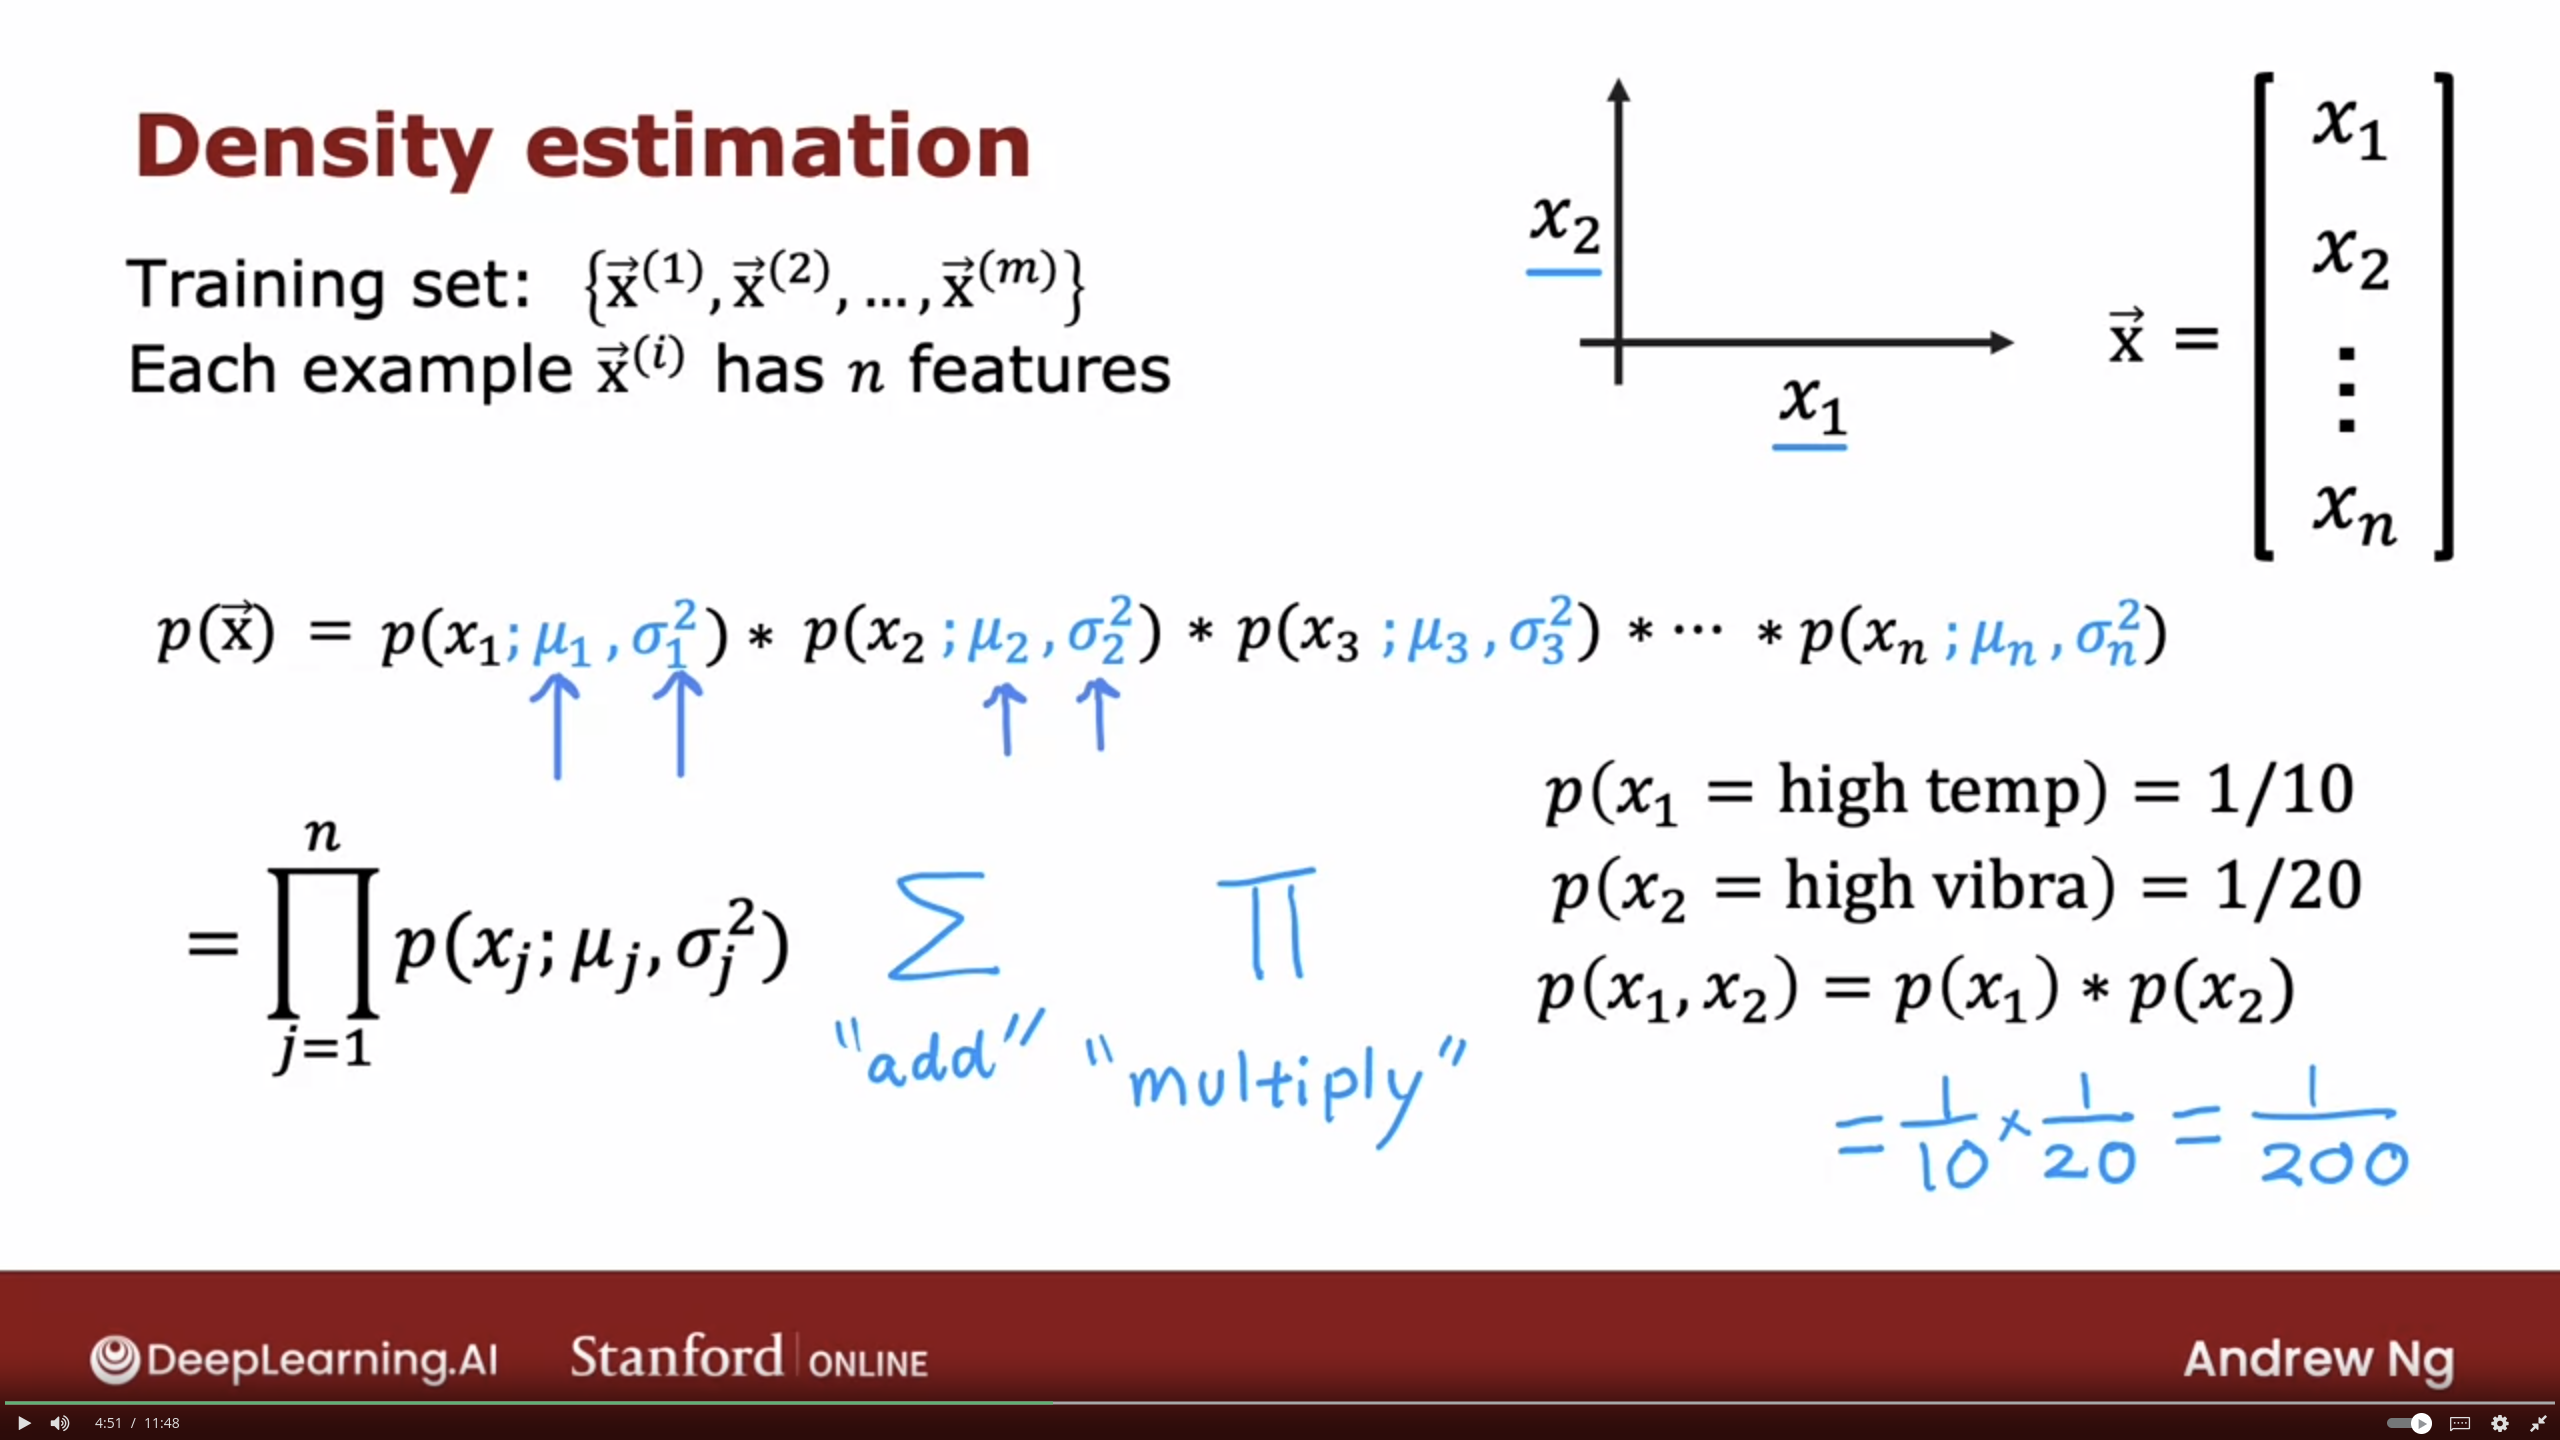
\includegraphics[trim =0.0cm 0.0cm 0.0cm 0.0cm, clip, scale=0.15]{pics/anomaly.png}
  \caption{Gaussian distribution}
  %{\footnotesize\textbf{Notes:} XXX.} % changed <<<<<<<<<<
  %#\label{XXX}
\end{figure}

In summary, here are the steps for anomaly detection:

\begin{figure}[H]
  \centering
  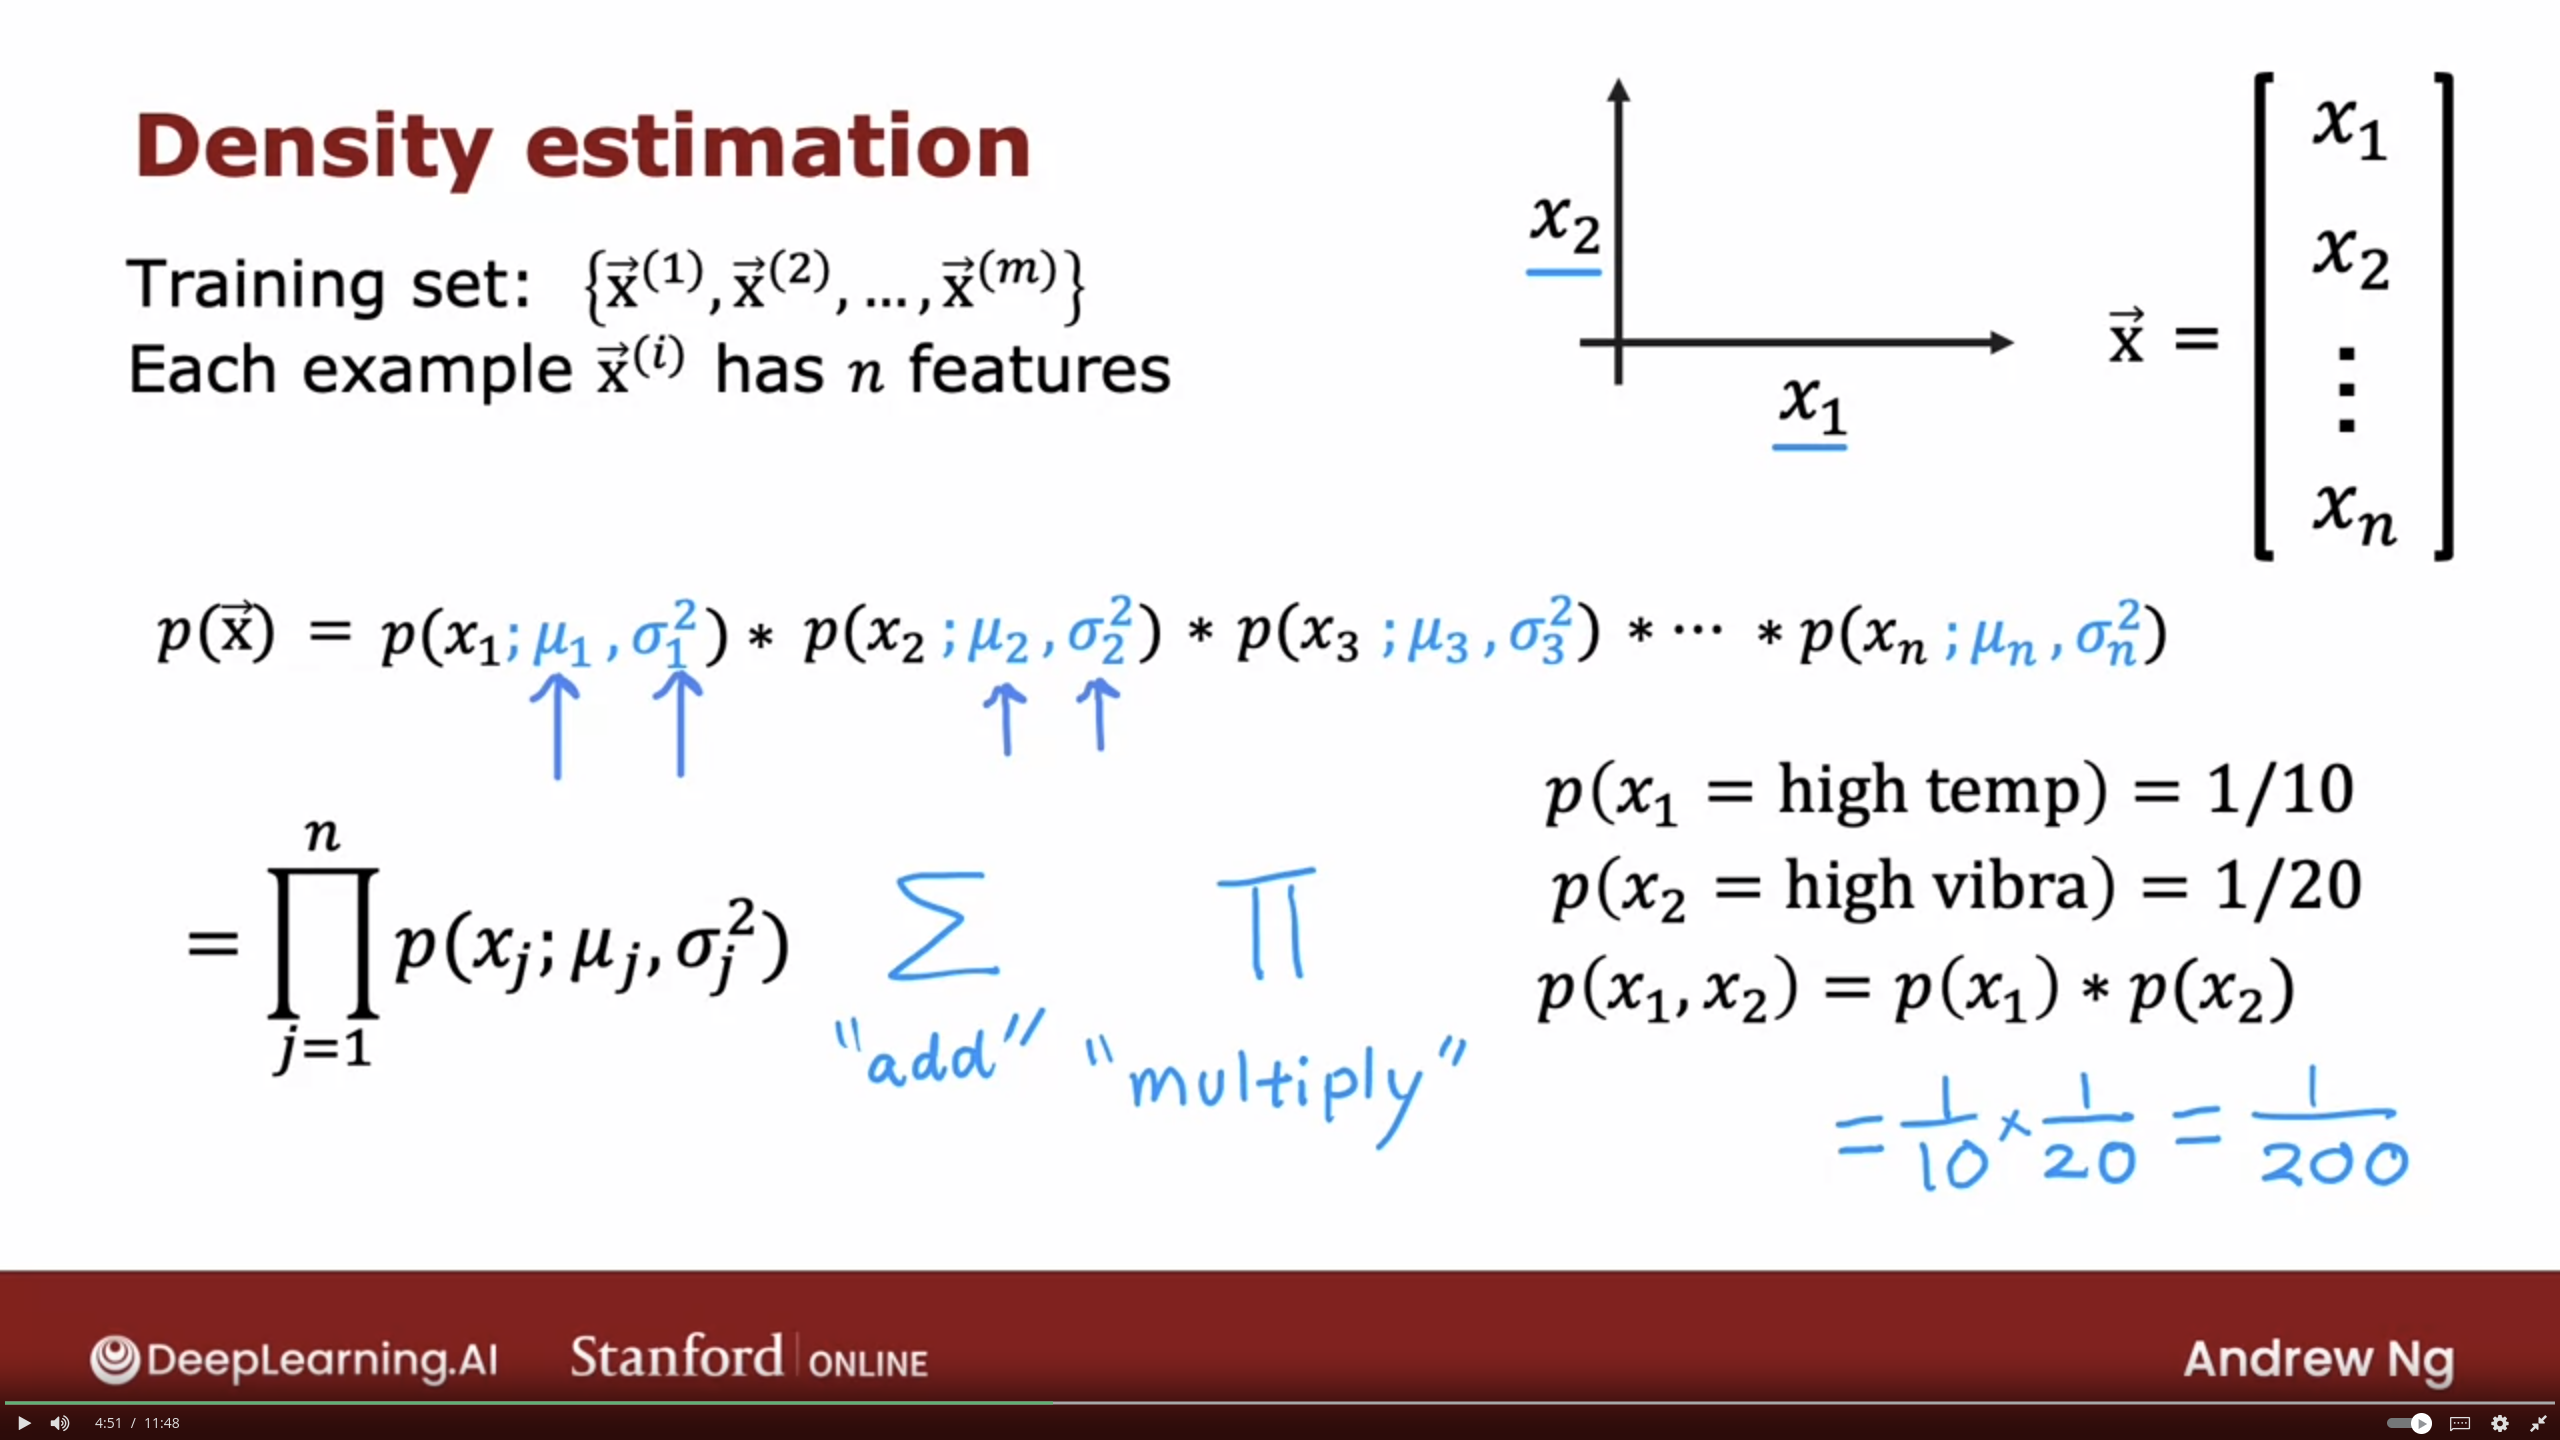
\includegraphics[trim =0.0cm 0.0cm 0.0cm 0.0cm, clip, scale=0.15]{pics/anomaly.png}
  \caption{Gaussian distribution}
  %{\footnotesize\textbf{Notes:} XXX.} % changed <<<<<<<<<<
  %#\label{XXX}
\end{figure}


To train the anomaly detection system, as always, we need to partition the data set. Let's say we have a data set with 10000 normal cases and 20, anomalies. We can partition the data as follows, then we use the training set to find $\mu \& \sigma^2$, and we use the cross validation algorithm to find and tune $\epsilon$ and even add or subtract some features. The test set is to report on the accuracy of the model, but if the set is small, we can skip the test set, and put all the anomalies in the cross validation set.

\begin{figure}[H]
  \centering
  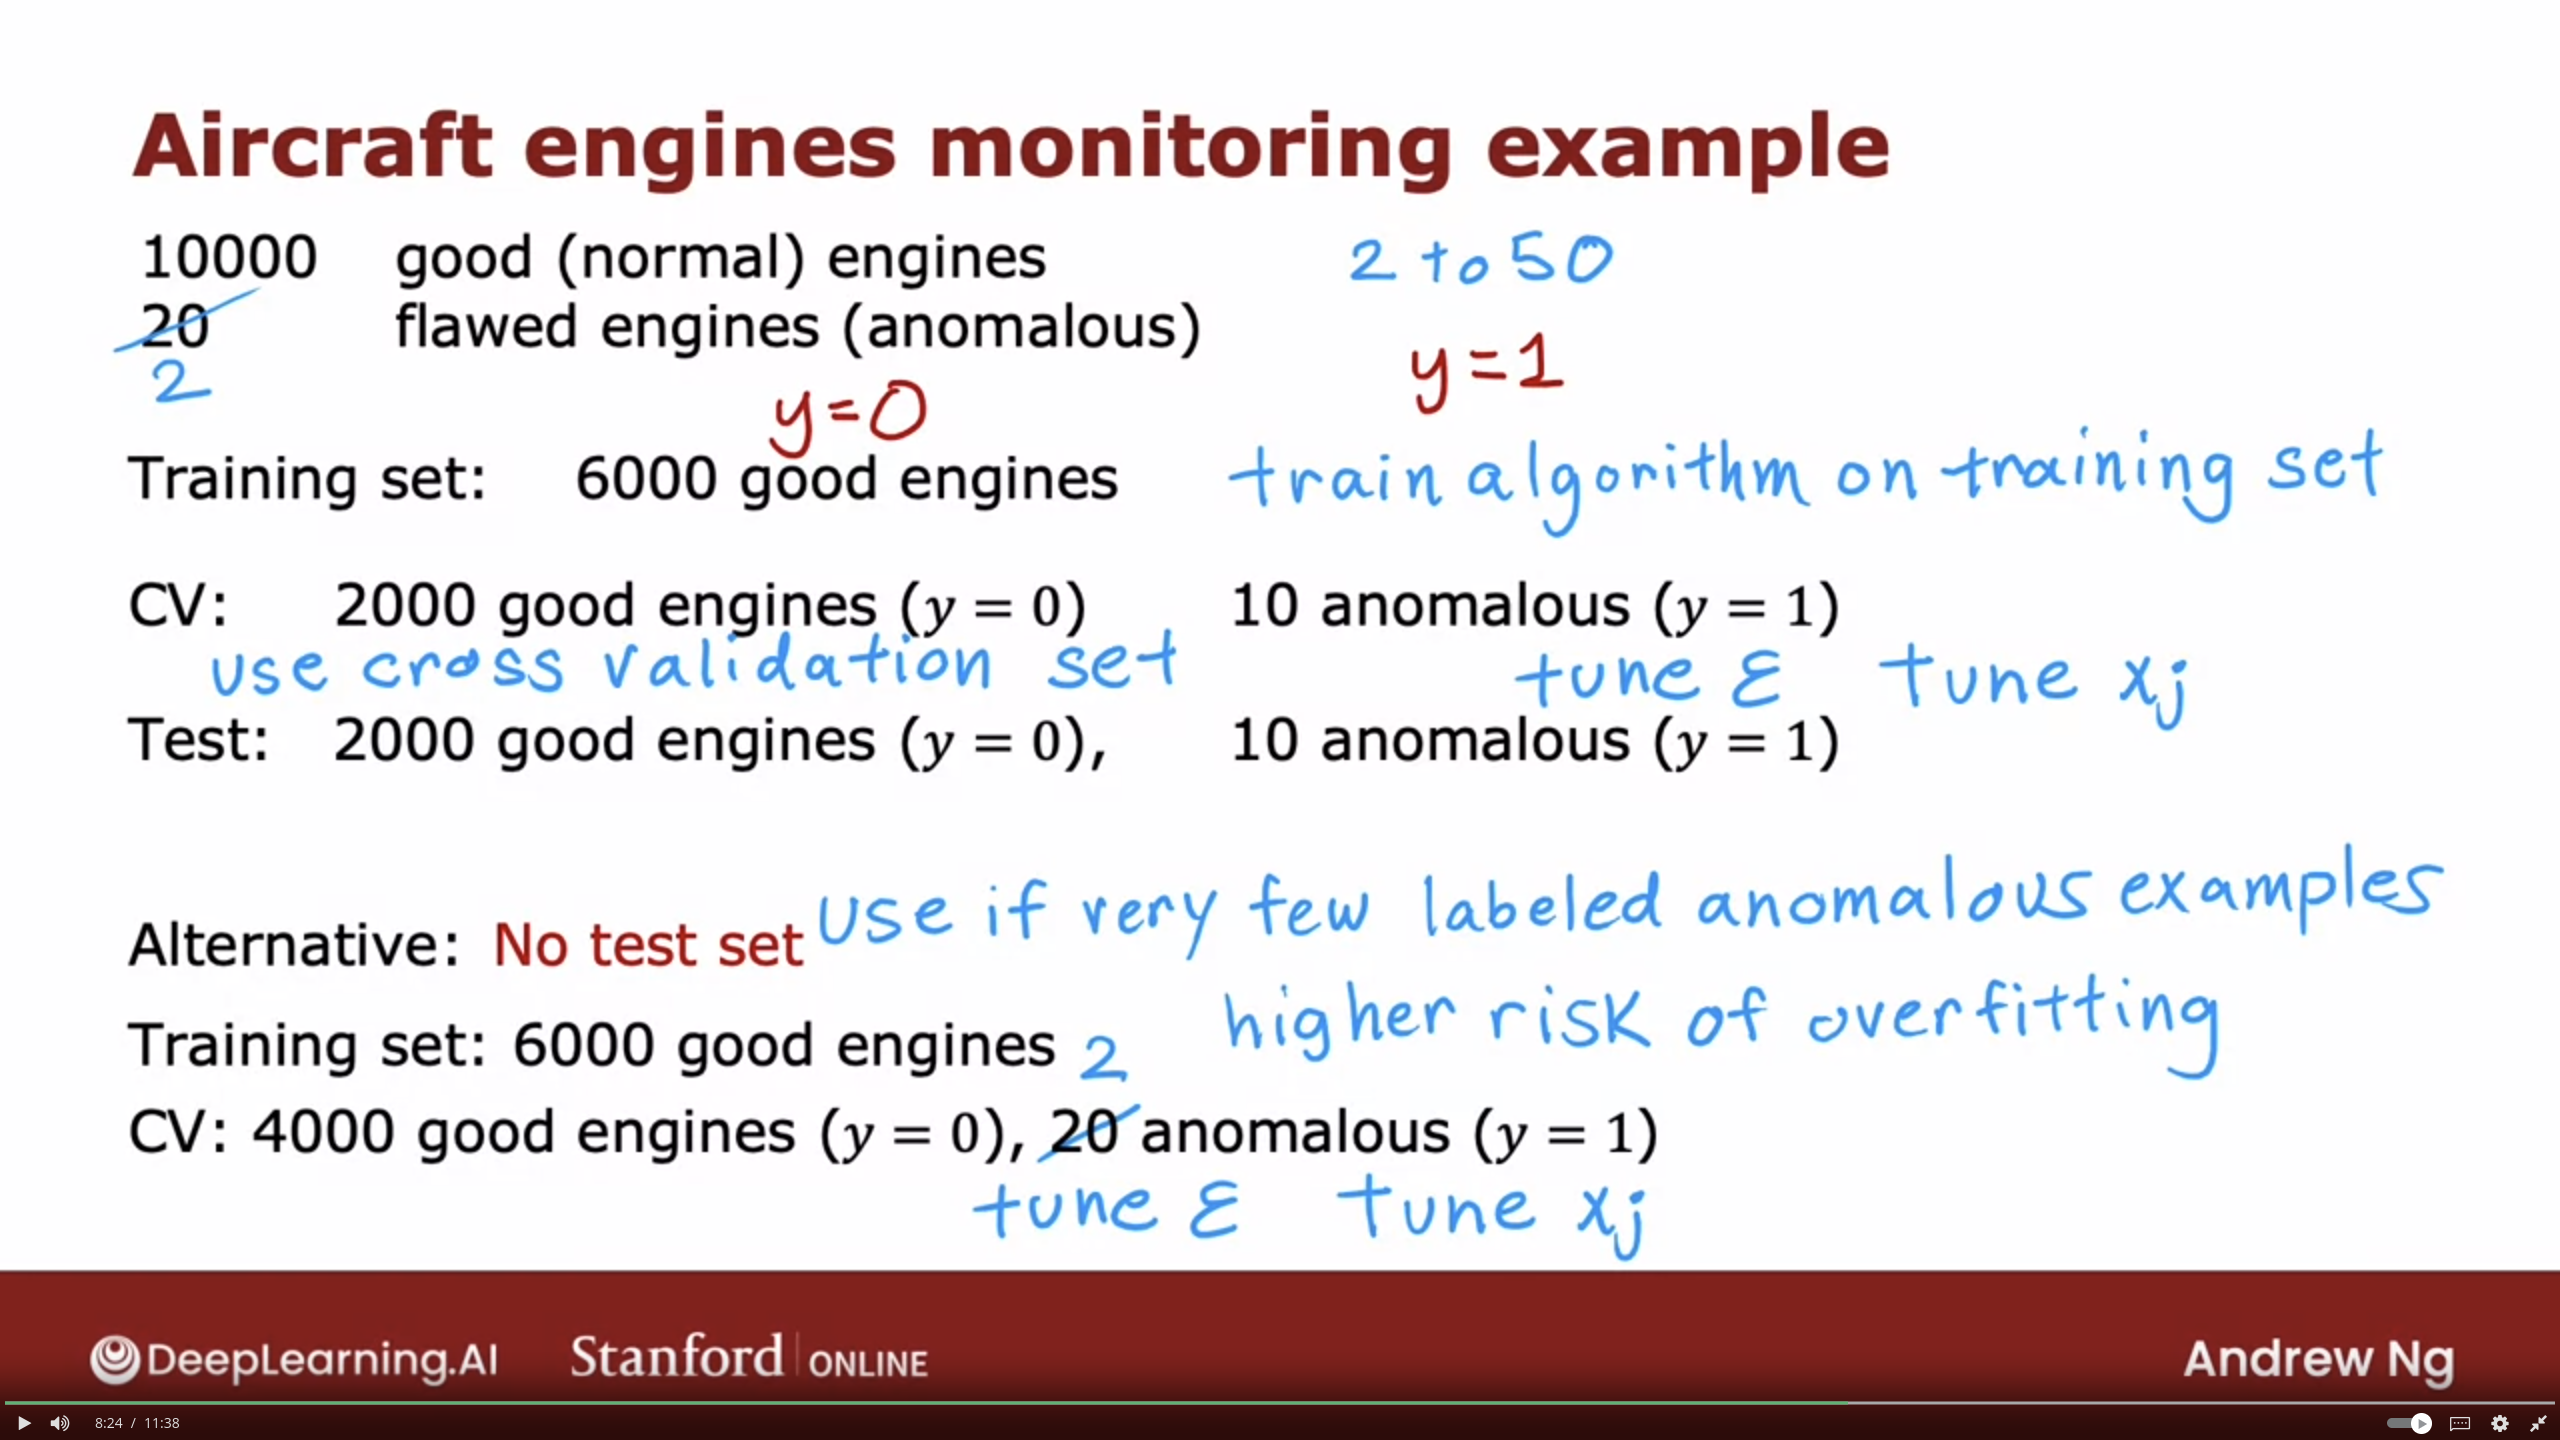
\includegraphics[trim =0.0cm 0.0cm 0.0cm 0.0cm, clip, scale=0.15]{pics/anomalymodel.png}
  \caption{Gaussian distribution}
  %{\footnotesize\textbf{Notes:} XXX.} % changed <<<<<<<<<<
  %#\label{XXX}
\end{figure}

To predict the accuracy of the model, we use the cross/test sets and see how many anomalies are flagged, and how many normal engines are flagged as anomalies.


This is still an unsupervised approach, because, technically samples don't have a label, but we just have a few anomalies labels. The question is why if we have anomalies label, not to use a supervised approach then. The way anomaly detection looks at the data set versus the way supervised learning looks at the data set are quite different. If you think there are many different types of anomalies or many different types of positive examples, then anomaly detection might be more appropriate. If there may be a brand new way anomaly then your 20 say positive examples may not cover all of the anomaly types. That makes it hard for any algorithm to learn from the small set of positive examples. And future anomalies may look nothing like any of the anomalous examples we've seen so far. If you believe this to be true for your problem, then I would gravitate to using an anomaly detection algorithm rather than supervised learning. In contrast, if there are enough positive examples that cover all types of anomalies, then a supervised algo is more appropriate. Anomaly detection tries to find brand new types that might not have been seen before.

In anomaly detection, choosing the features is one main question (this is not the case with supervised learning, as less important features will phase out in the learning process). Features should be Gaussian, and if they are not, we should change them to be look like more to Gaussian distribution:

\begin{figure}[H]
  \centering
  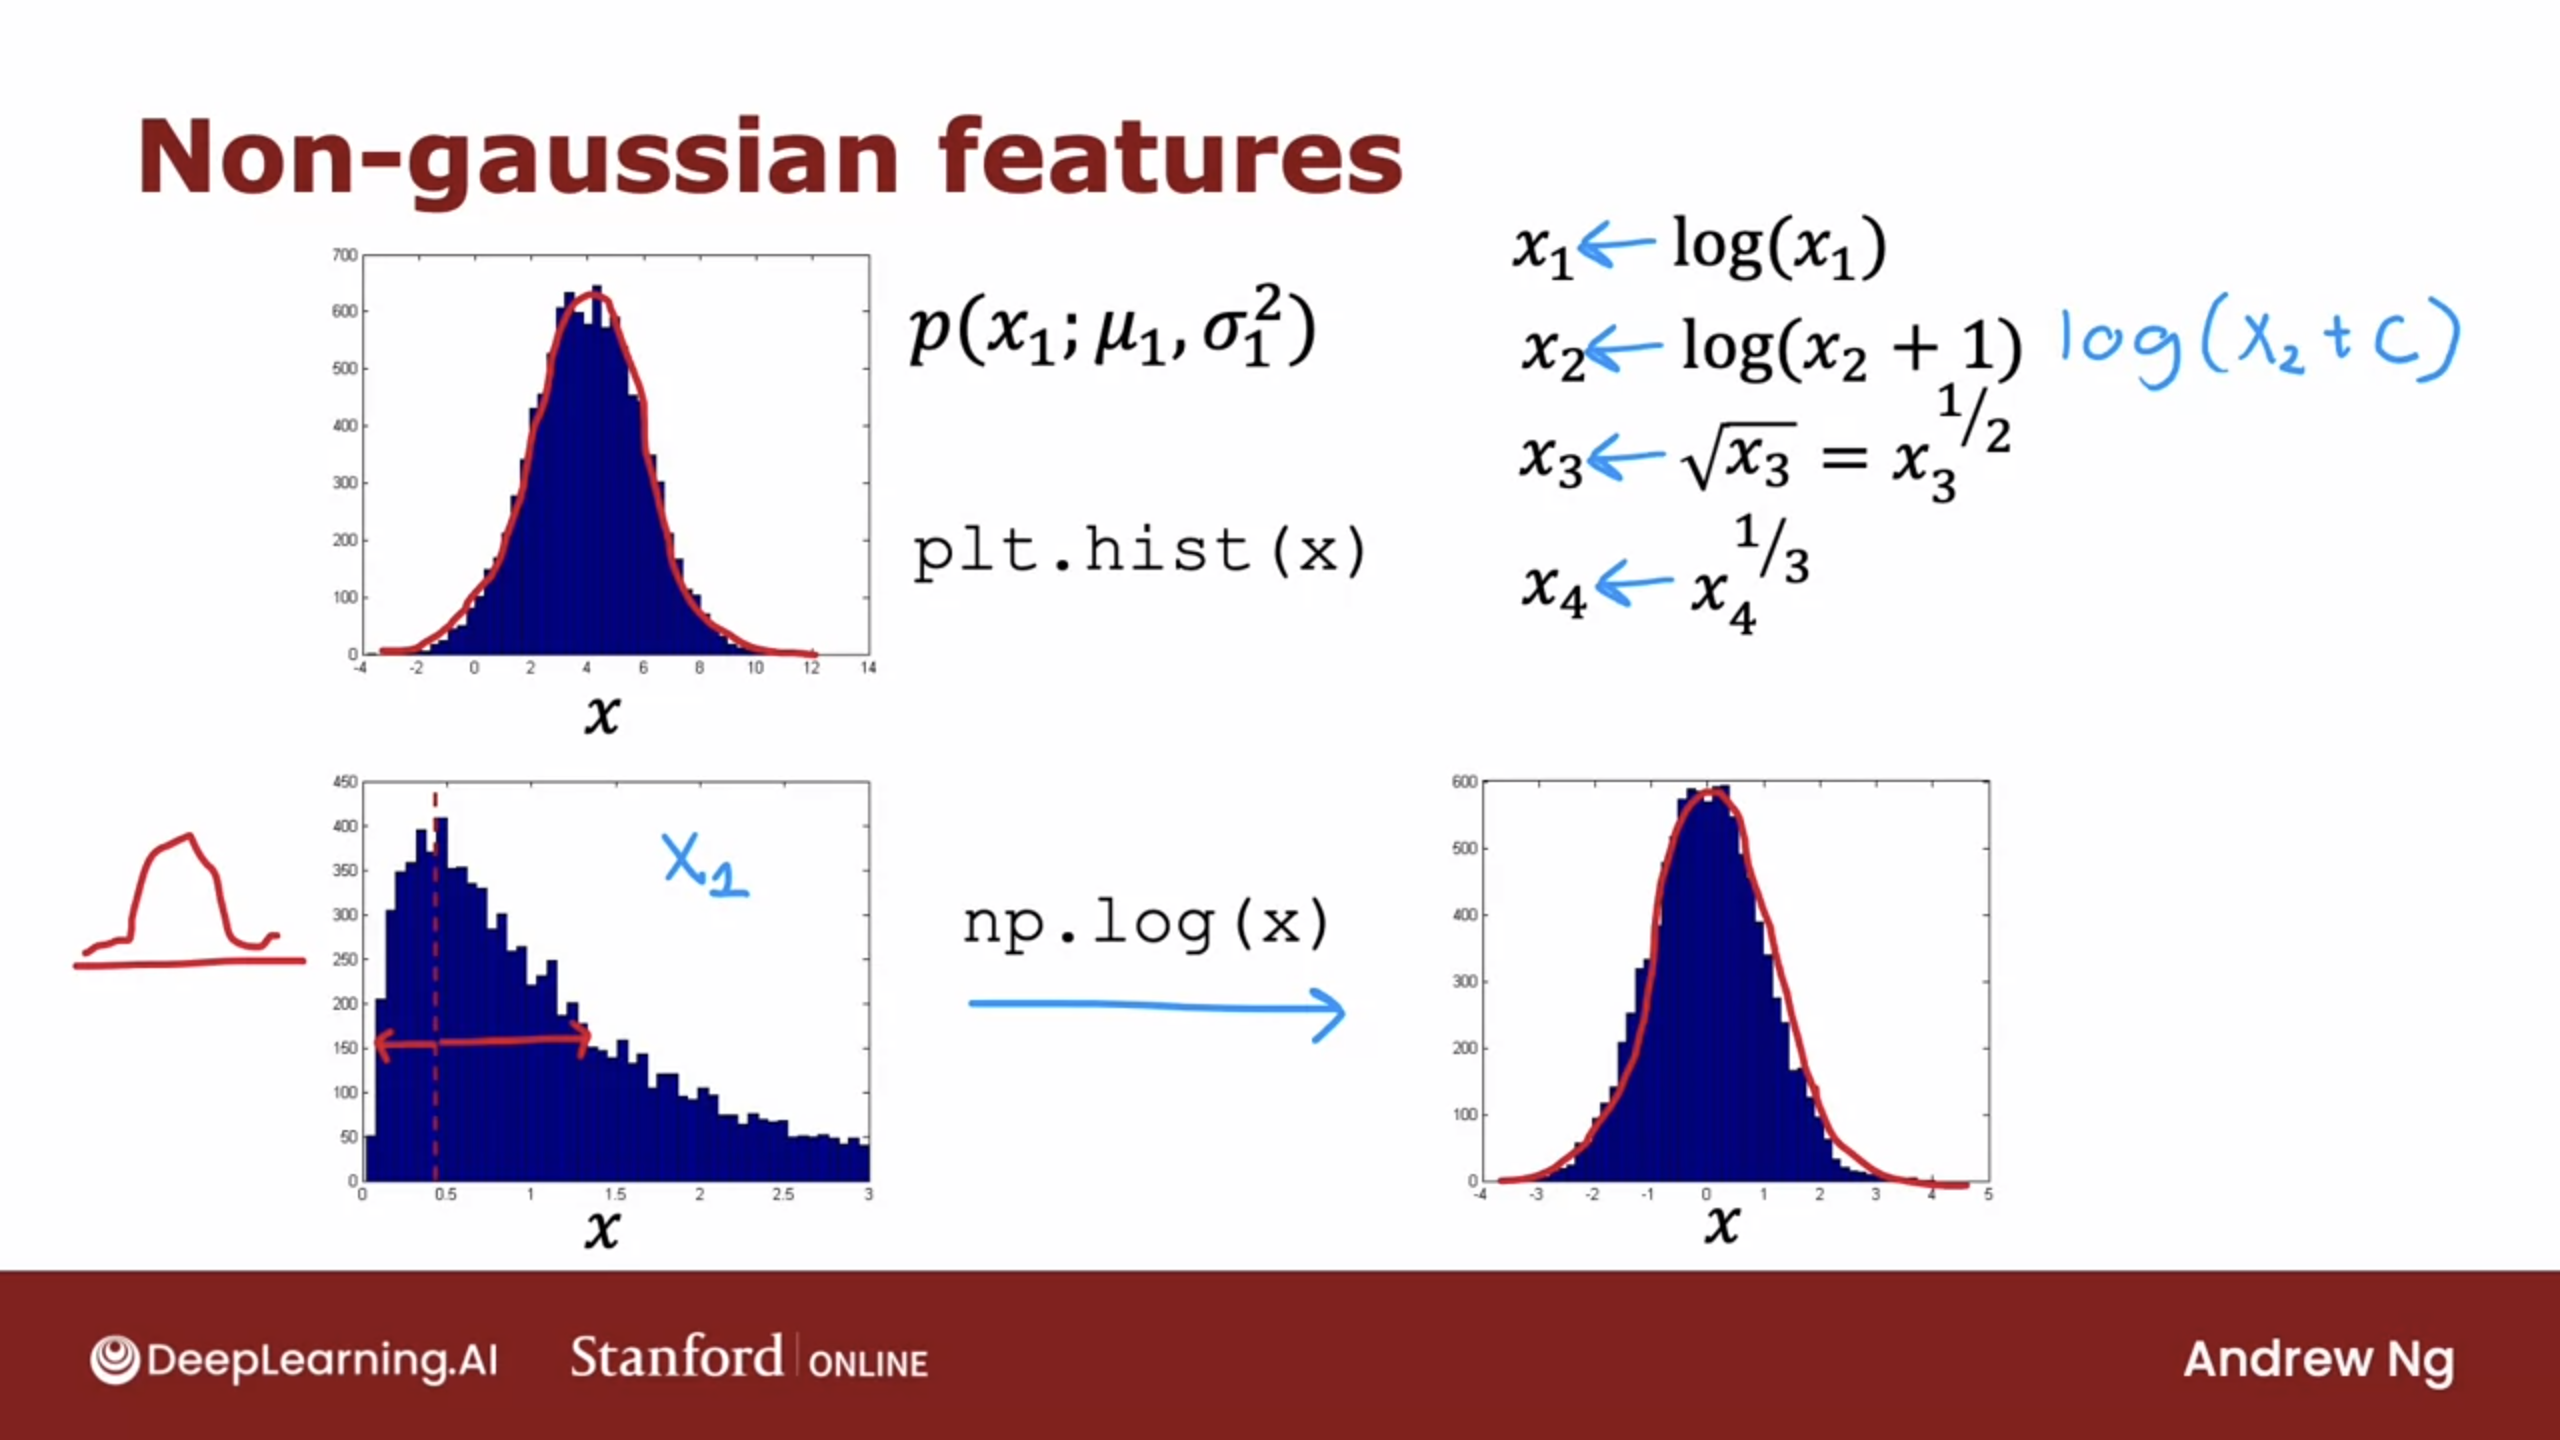
\includegraphics[trim =0.0cm 0.0cm 0.0cm 0.0cm, clip, scale=0.15]{pics/convertToGaussian.png}
  \caption{Gaussian distribution}
  %{\footnotesize\textbf{Notes:} XXX.} % changed <<<<<<<<<<
  %#\label{XXX}
\end{figure}




\chapter[Reinforced Learning]{Reinforced Learning (RL)}

\section{Markov Decision Process}

\chapter[Large Language Models (LLM) and Transformers]{Large Language Models (LLM) and Transformers}

\section{Introduction}

Generative AI: A type of AI that can produce various types of content, including text, imagery, audio, and synthetic data based on what it has learned from existing content. Gen AI is a subset of Deep Learning, which uses Artificial Neural Networks, can process both labeled and unlabeled data, using supervised, unsupervised, and semi-supervised methods.


DL/ML can be divided into two types: generative and discriminative/predictive. \textbf{Discriminative model} is used to classify or predict labels for data points. They are typically trained on a dataset of labeled data points, and they learn the relationship between the features of the data points and the labels. After training, discriminative models can be used to predict/cluster/classify  the label for new data points. \textbf{A generative model }generates new data instances based on a learned probability distribution of existing data.

In short, the output of a discriminative model is a number, probability, class, and discrete. But the output of generative AI is natural language, audio, or image.


The power of Generative AIs is coming from transformers, announced for the first time in a paper called "Attention is all you need", which proposed a neural network architecture that replaces traditional recurrent neural networks (RNN and CNN).
The Transformer architecture consists of an encoder and a decoder, each of which is composed of several layers. Each layer consists of two sub-layers: a multi-head self-attention mechanism and a feed-forward neural network. The multi-head self-attention mechanism allows the model to attend to different parts of the input sequence, while the feed-forward network applies a point-wise fully connected layer to each position separately and identically. The Transformer model also uses residual connections and layer normalization to facilitate training and prevent overfitting. In addition, the authors introduce a positional encoding scheme that encodes the position of each token in the input sequence, enabling the model to capture the order of the sequence without the need for recurrent or convolutional operations. A transformer is a special type of neural network.


\begin{figure}
  \centering
  \begin{subfigure}[] %{.5\textwidth}
    \centering
    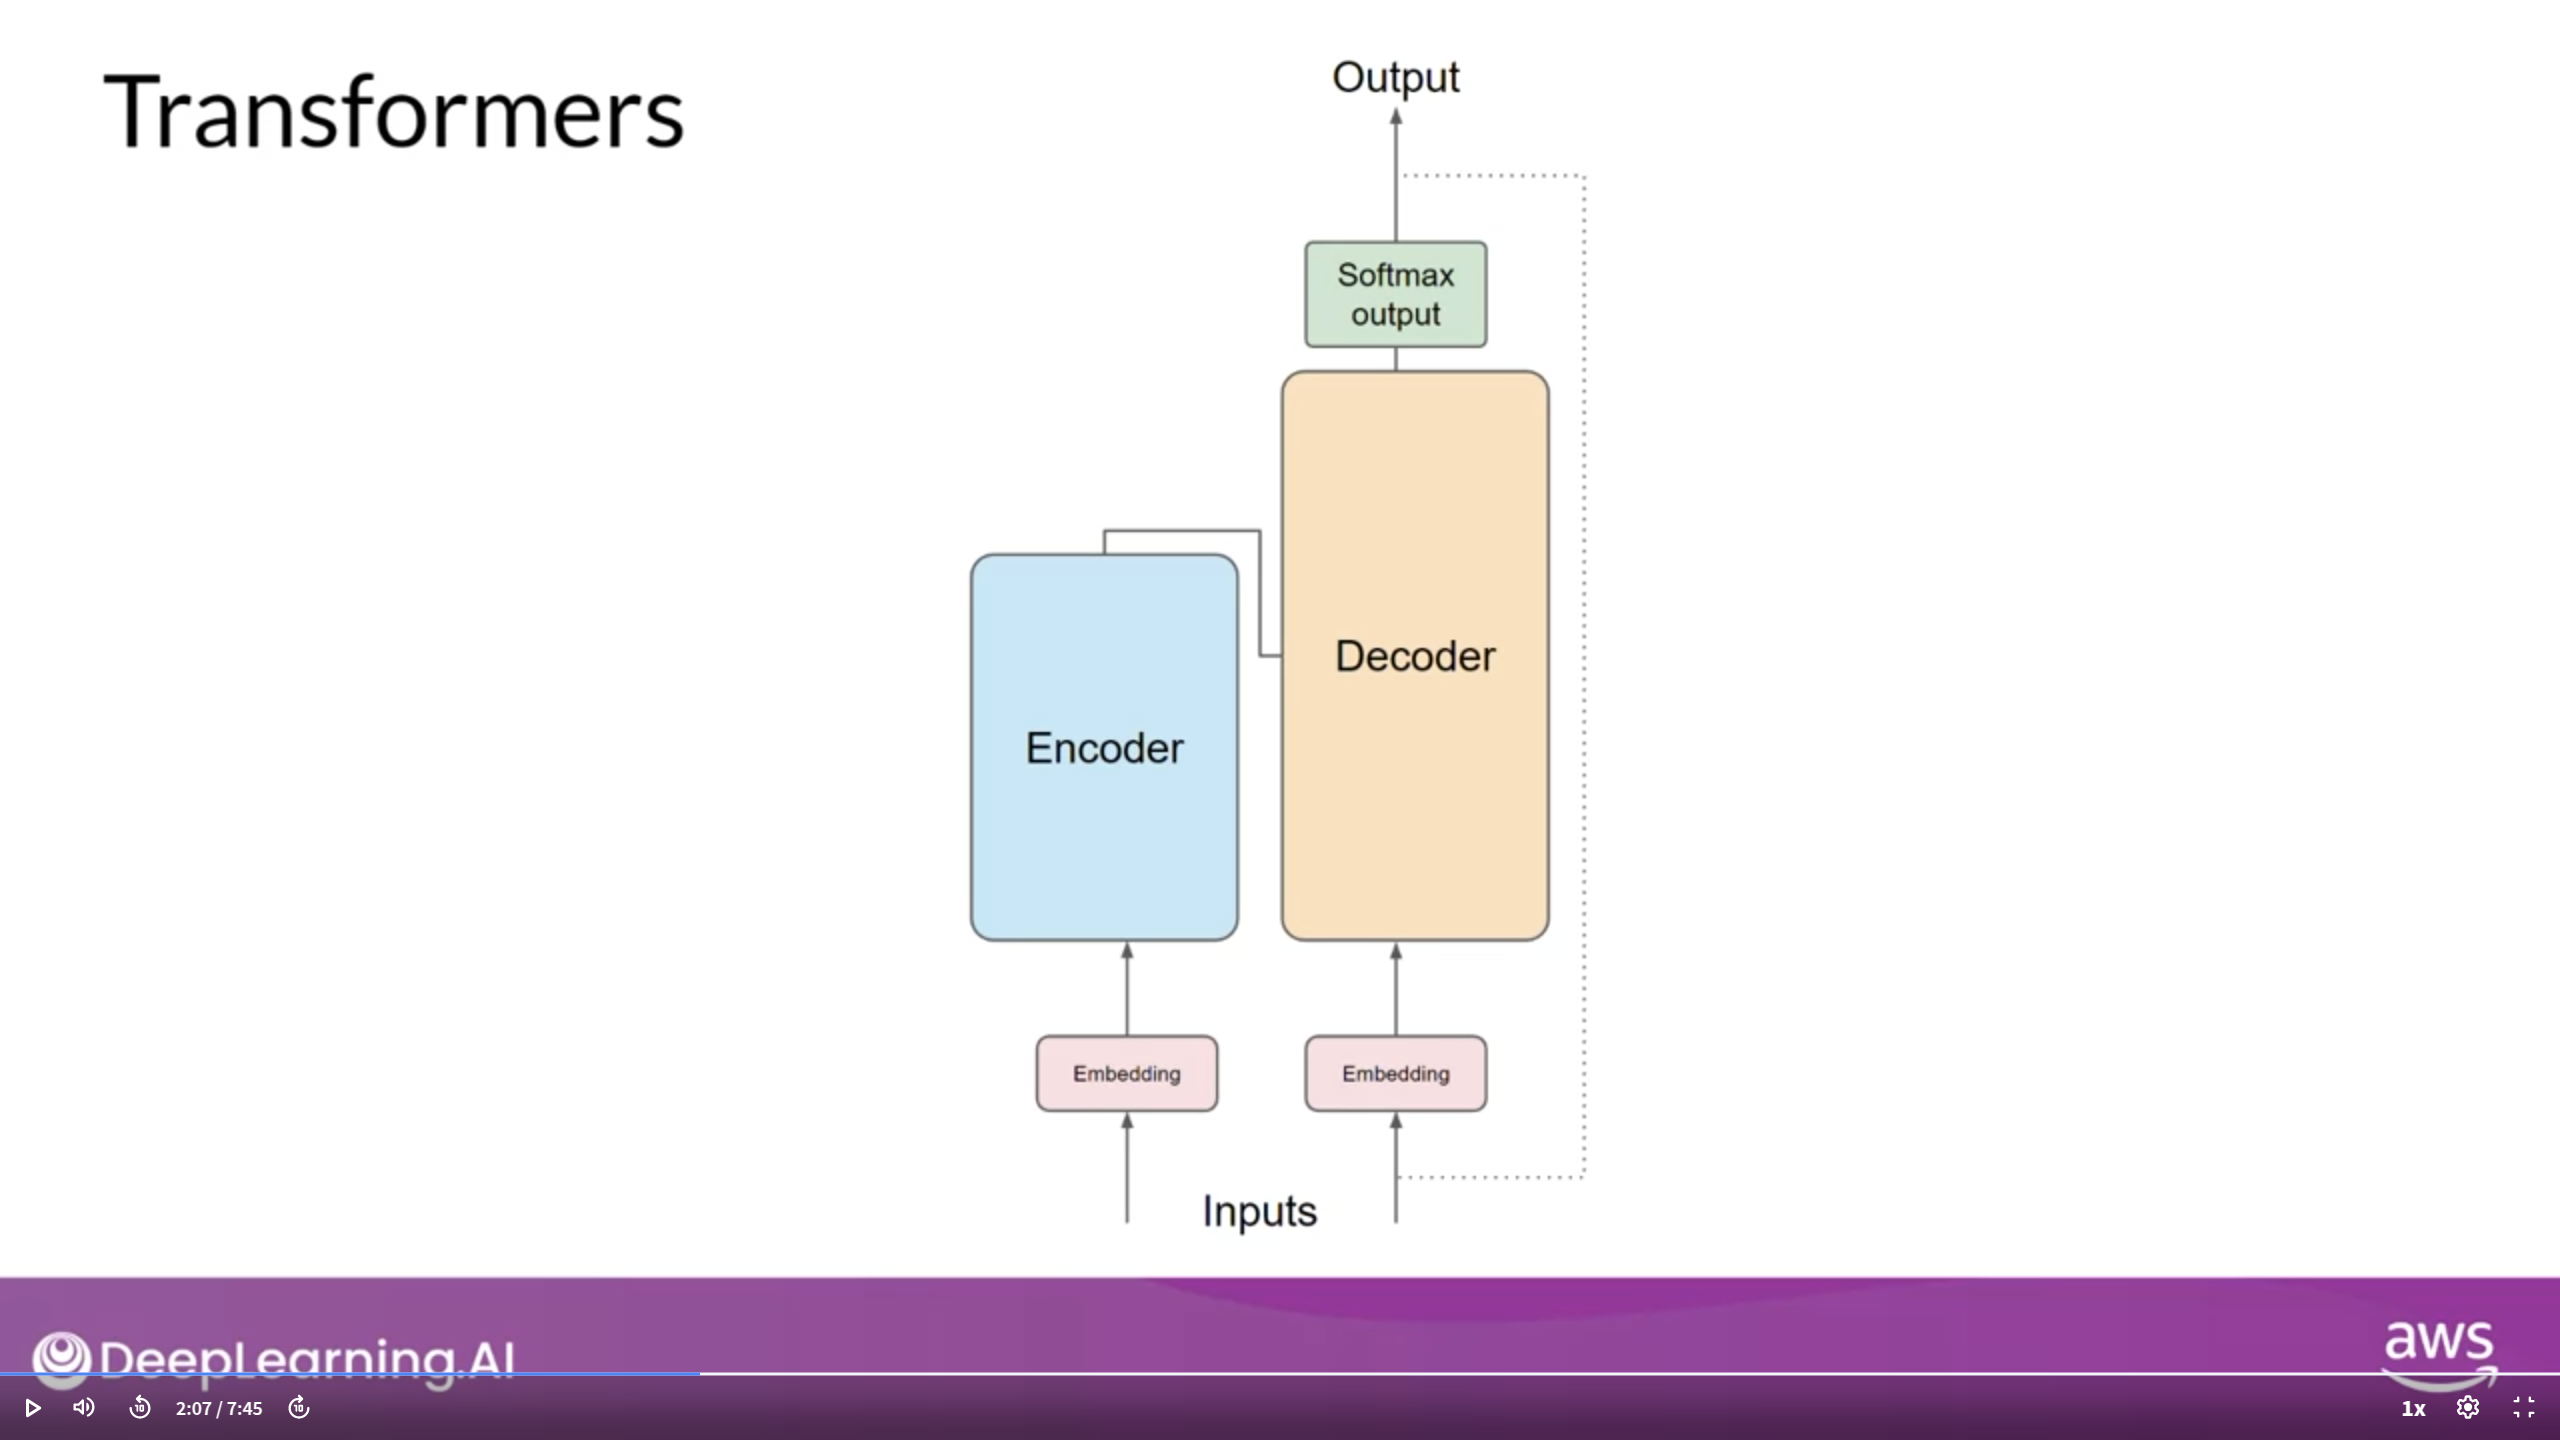
\includegraphics[trim=3cm 7cm 5cm 0cm,clip,scale=0.11]{pics/transformers.png}
    %\caption{}
    %\label{fig:sub1}
  \end{subfigure}%
  \begin{subfigure}[] % {.5\textwidth}
    \centering
    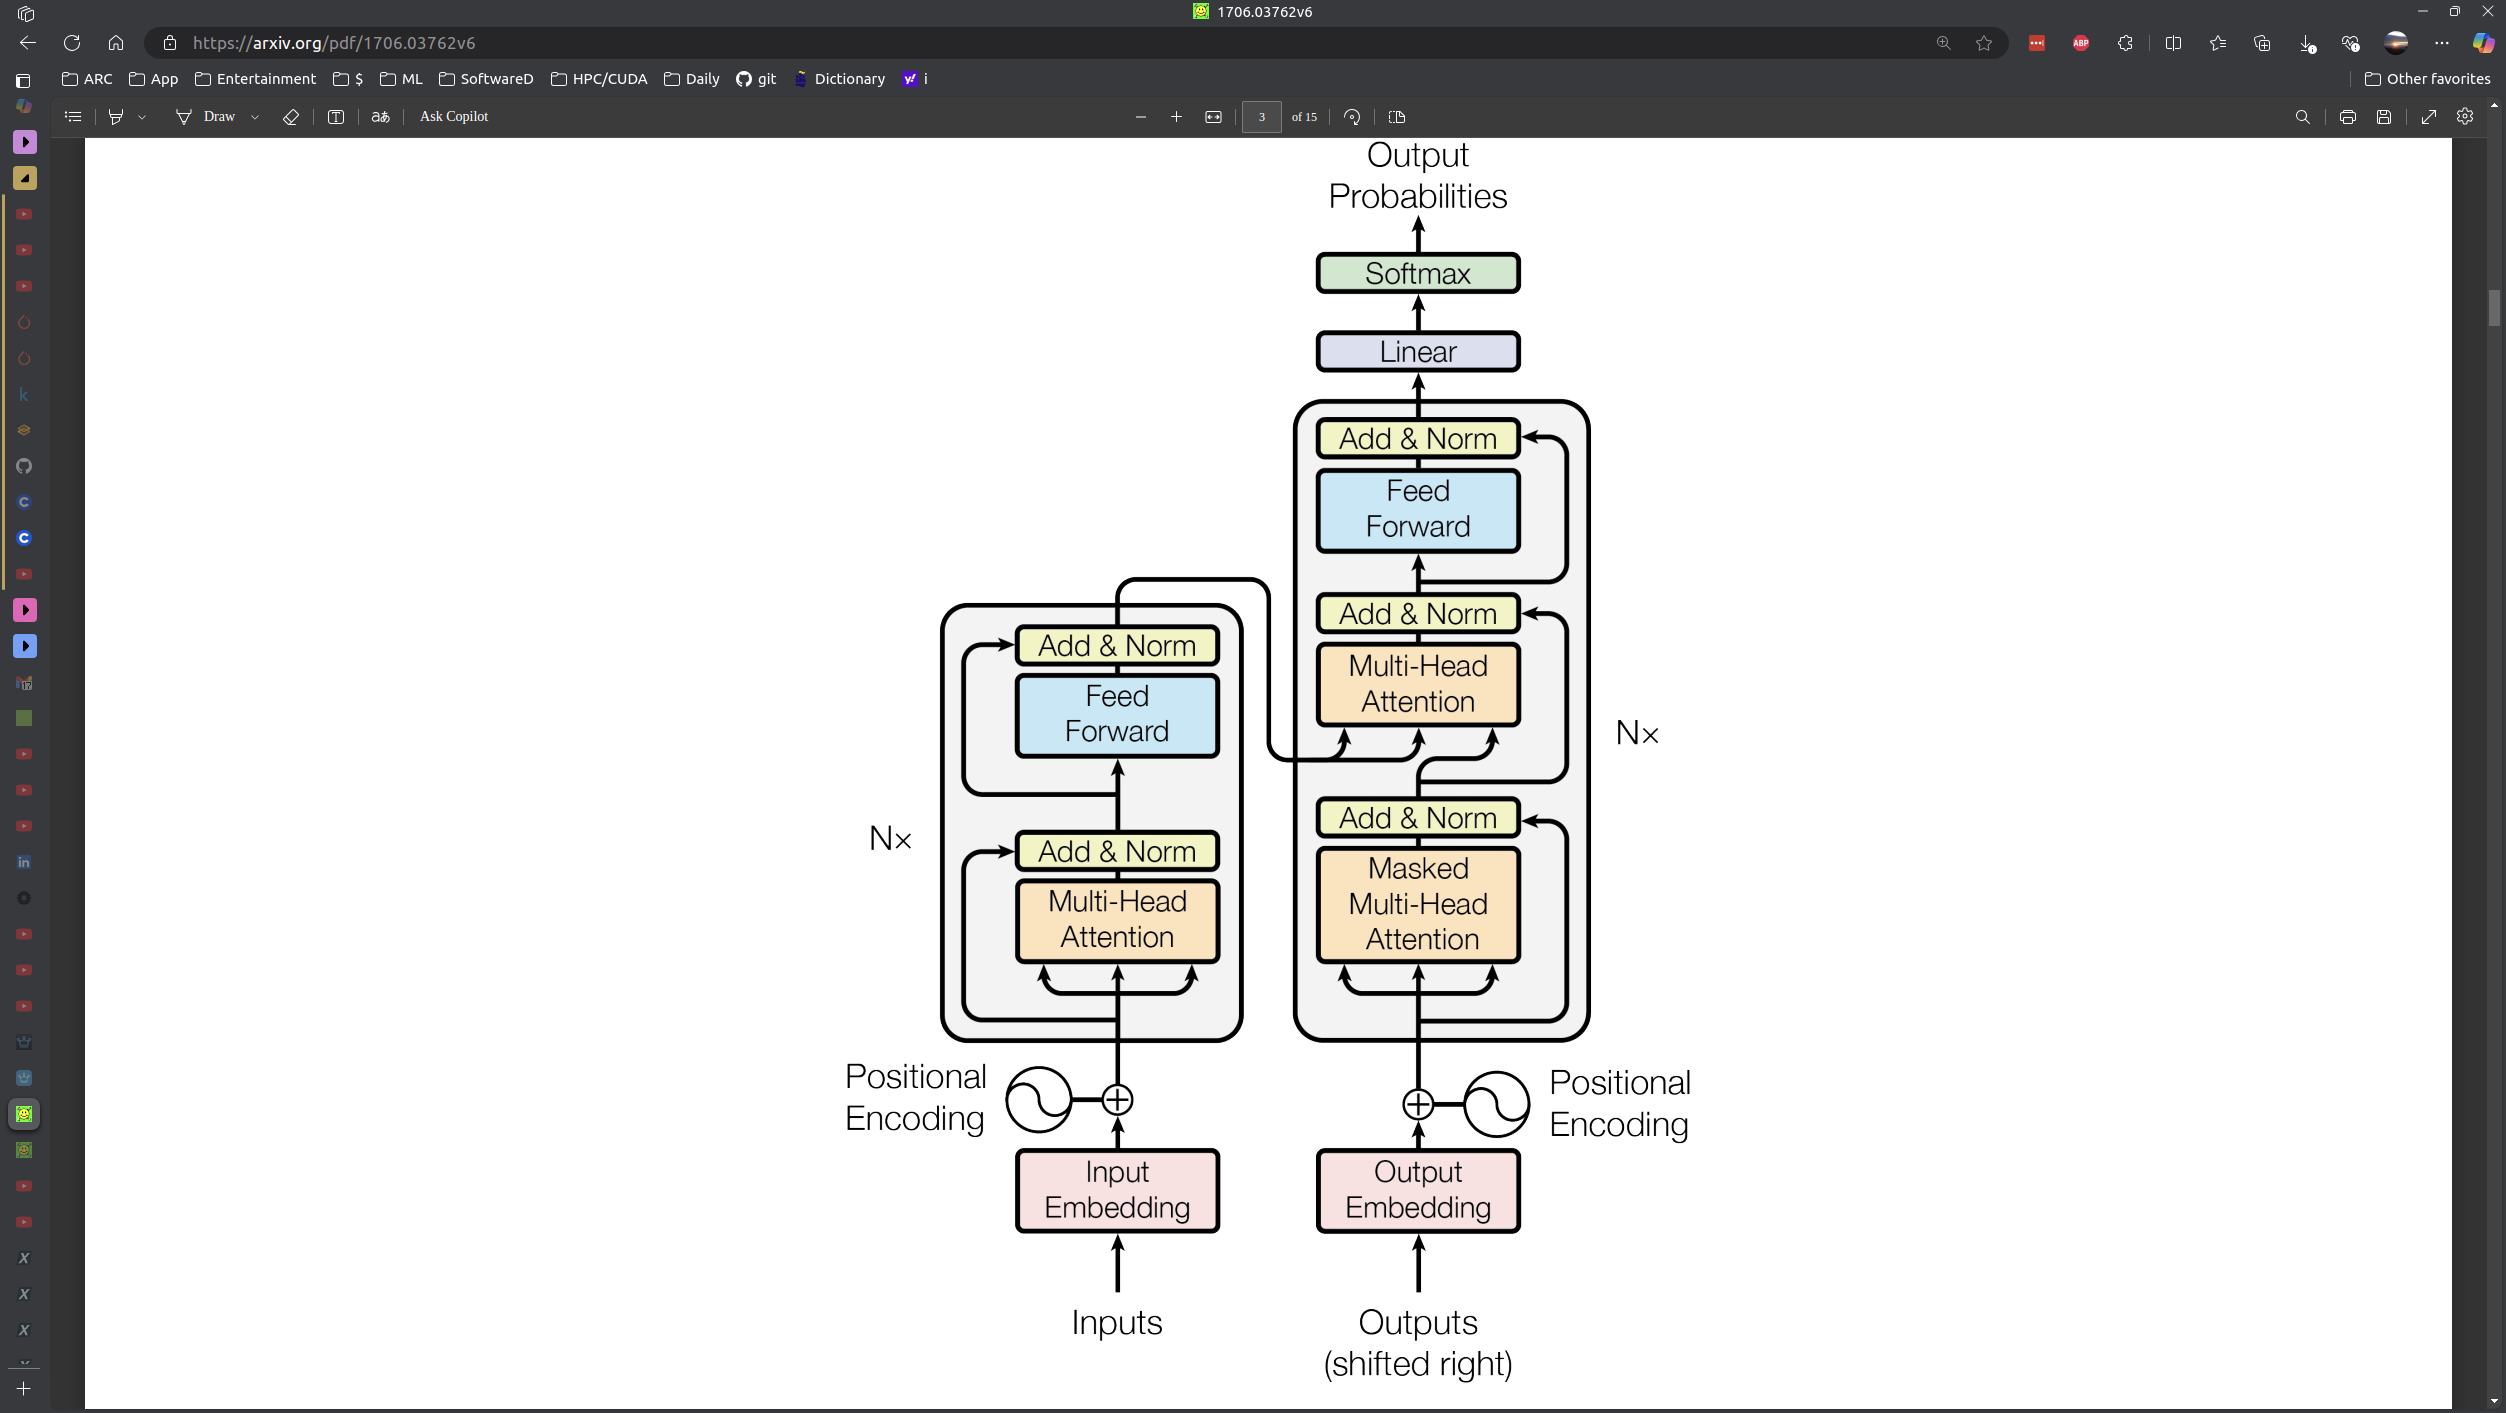
\includegraphics[trim=10cm 1cm 10cm 5cm,clip,scale=0.12]{pics/arch.png} %
    %\caption{}
    %%\label{fig:sub2}
  \end{subfigure}
  \caption{Transformer structure: (a) Encoder/decoder section, (b) Full picture}
  %\label{fig:test}
\end{figure}

Step 1:
ML models are just big statistical calculators and they work with numbers, not words. So, before passing texts into the model to process, you must first tokenize the words. This converts the words into numbers with each number representing a position in a dictionary of all the possible words that the model can work with. There are multiple tokenization methods. For example, token IDs matching the entire word, or using token IDs to represent parts of words. We need to use the same tokenizer for encoding and decoding.

Step 2:
Once the input is tokenized, you can pass it to the embedding layer. This is a trainable vector embedding in space. Each token ID is represented as a vector and is mapped to a multi dimensional vector. These vectors learn to encode the meaning and the context of the individual tokens in the input sequence. Words with similar meanings land in a space closer to each other.

\begin{figure}[H]
  \centering
  \caption{Embedded spaces in transformers}
  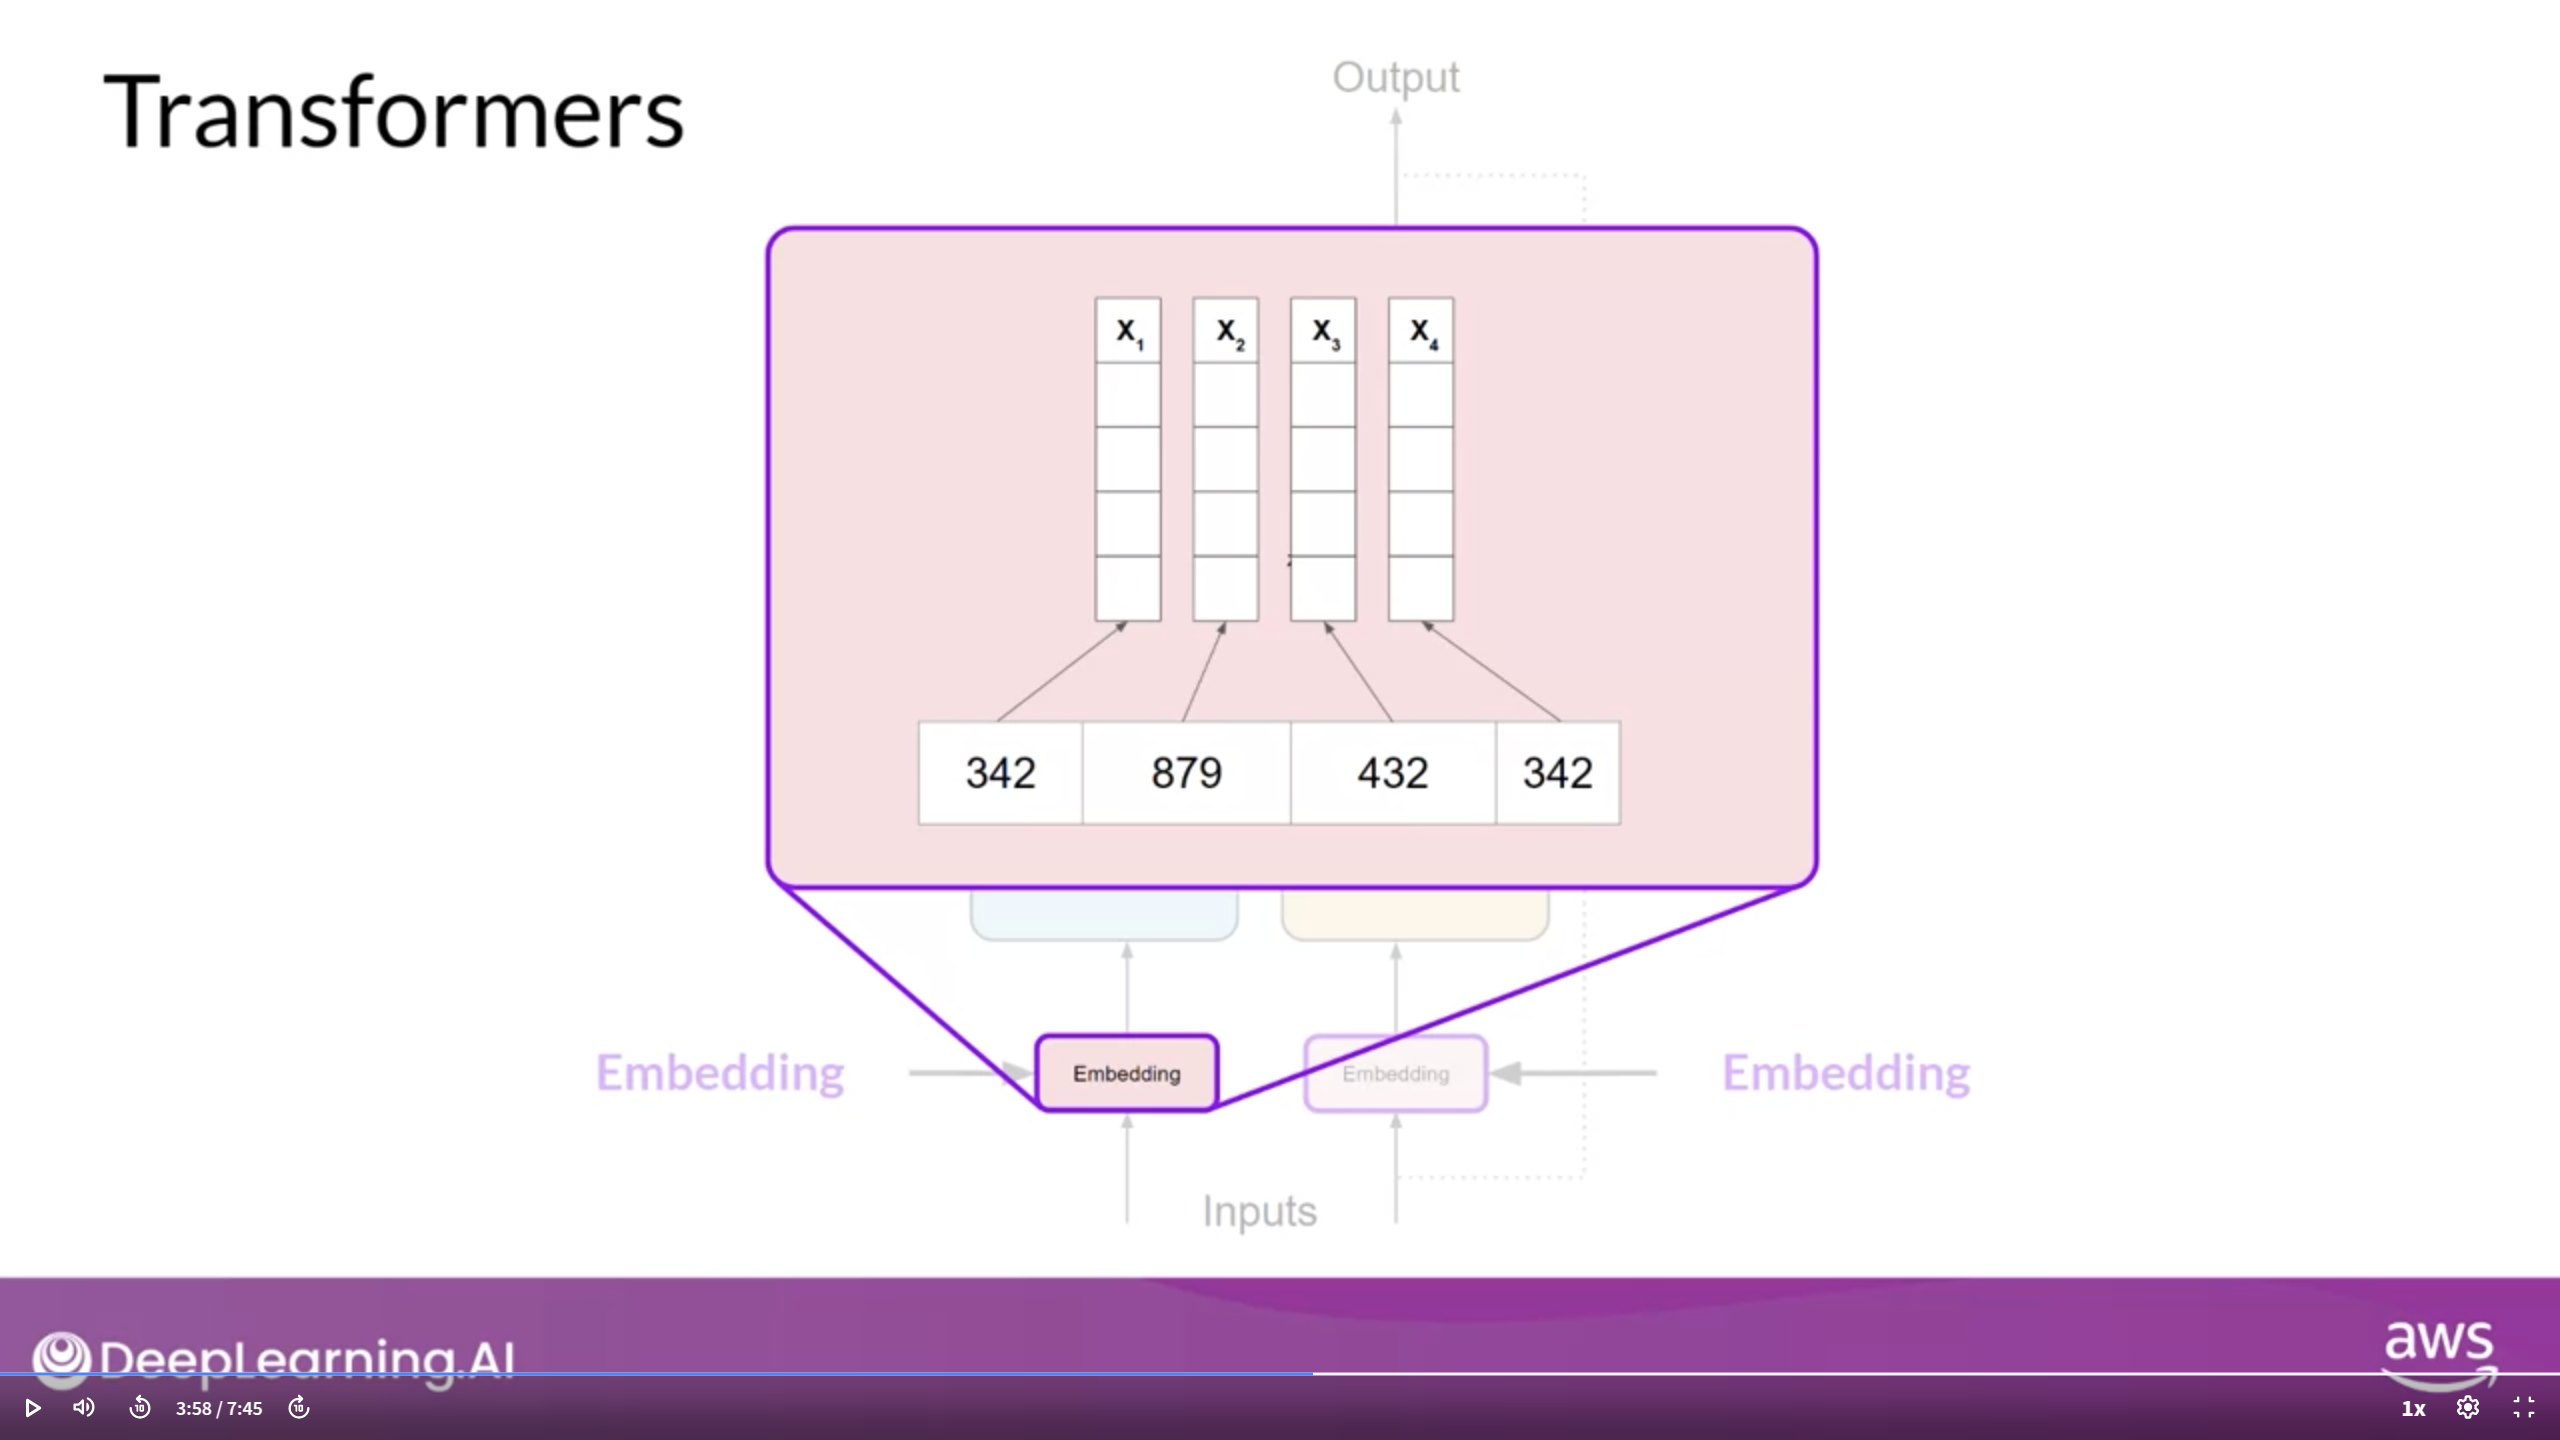
\includegraphics[trim=3cm 7cm 5cm 0cm,clip,scale=0.15]{pics/embeddedSpace.png}
  %{\footnotesize\textbf{Notes:} XXX.} % changed <<<<<<<<<<
  %#\label{XXX}
\end{figure}

The embedded space allows you to find the relation ship between spaces. For example, assume that the space is only three dimensional (the actual paper uses a 512-dimensional space.). Then, you find related words in the space.


\begin{figure}[H]
  \centering
  \caption{Example of embedded spaces}
  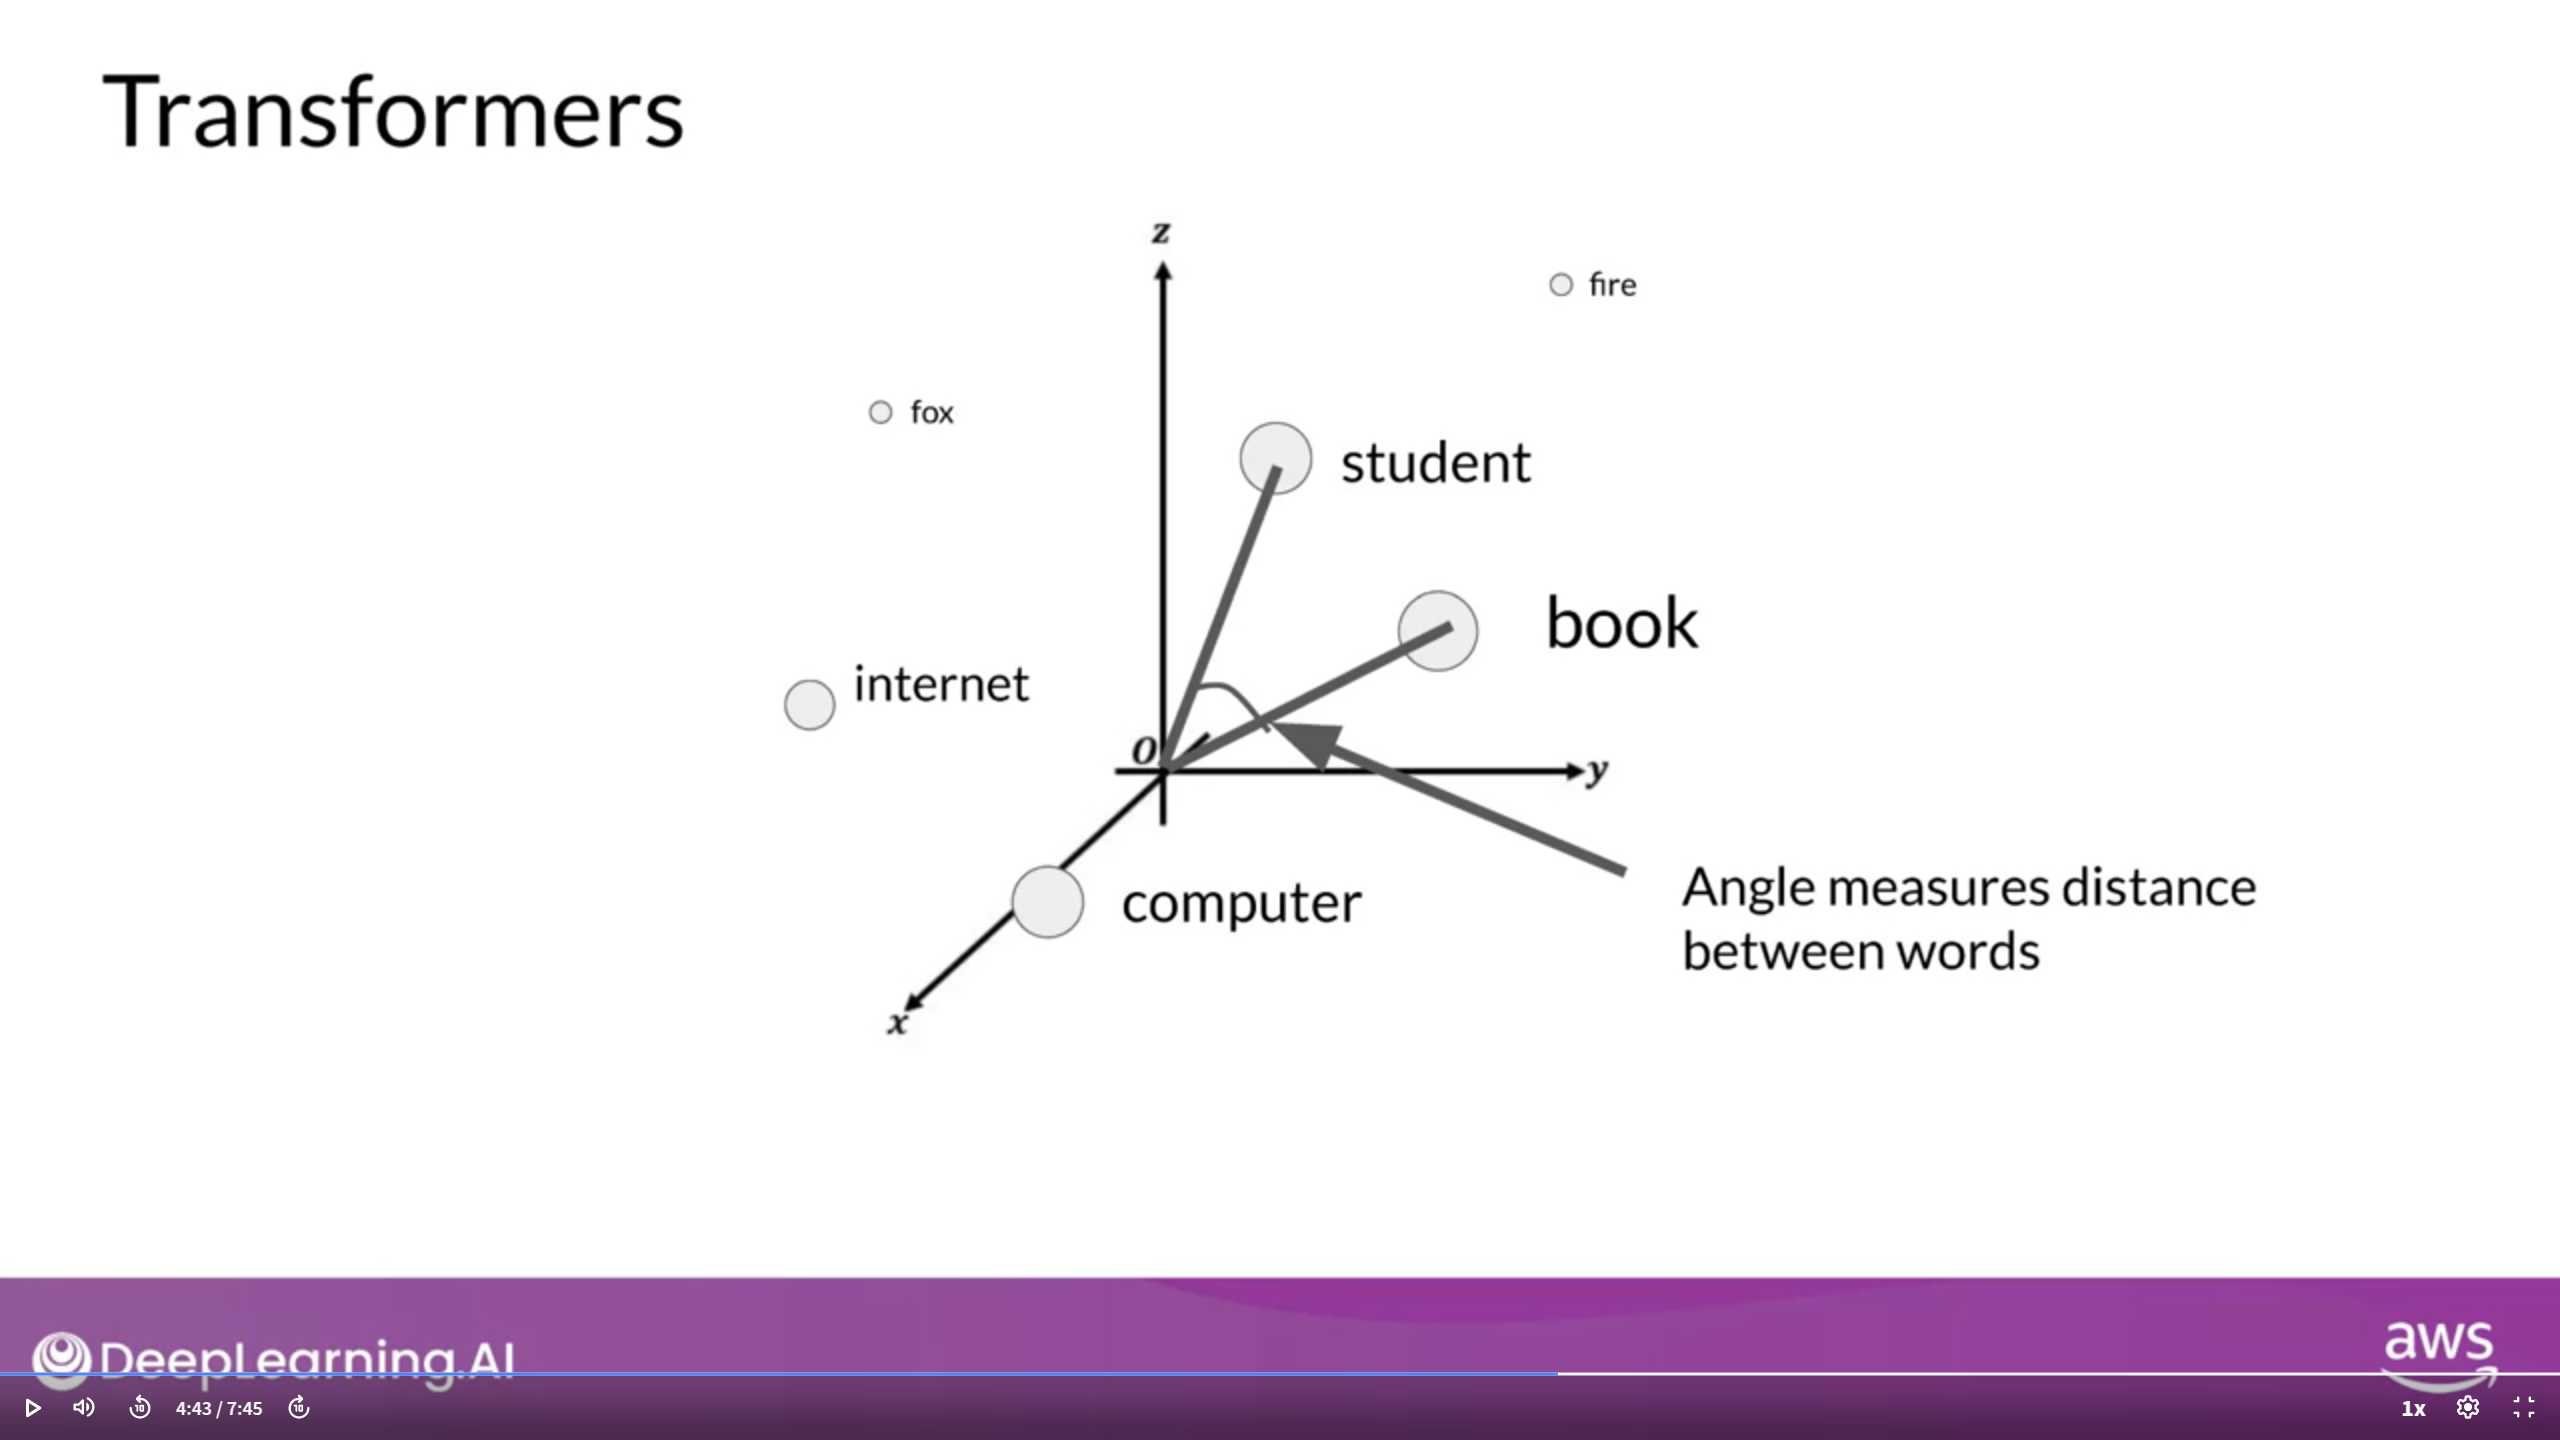
\includegraphics[trim=3cm 7cm 5cm 0cm,clip,scale=0.15]{pics/exEmbedSpace.png}
  %{\footnotesize\textbf{Notes:} XXX.} % changed <<<<<<<<<<
  %#\label{XXX}
\end{figure}


Step 3: Positional encoding. The model processes each of the input tokens in parallel. So, bu adding the positional encoding, you preserve the information about the word order and don't lose the relevance of the position of the word in the sentence. Once you summed the input tokens and the positional encodings, you pass the resulting vectors to the self-attention layer.

\begin{figure}[H]
  \centering
  \caption{Positional encoding}
  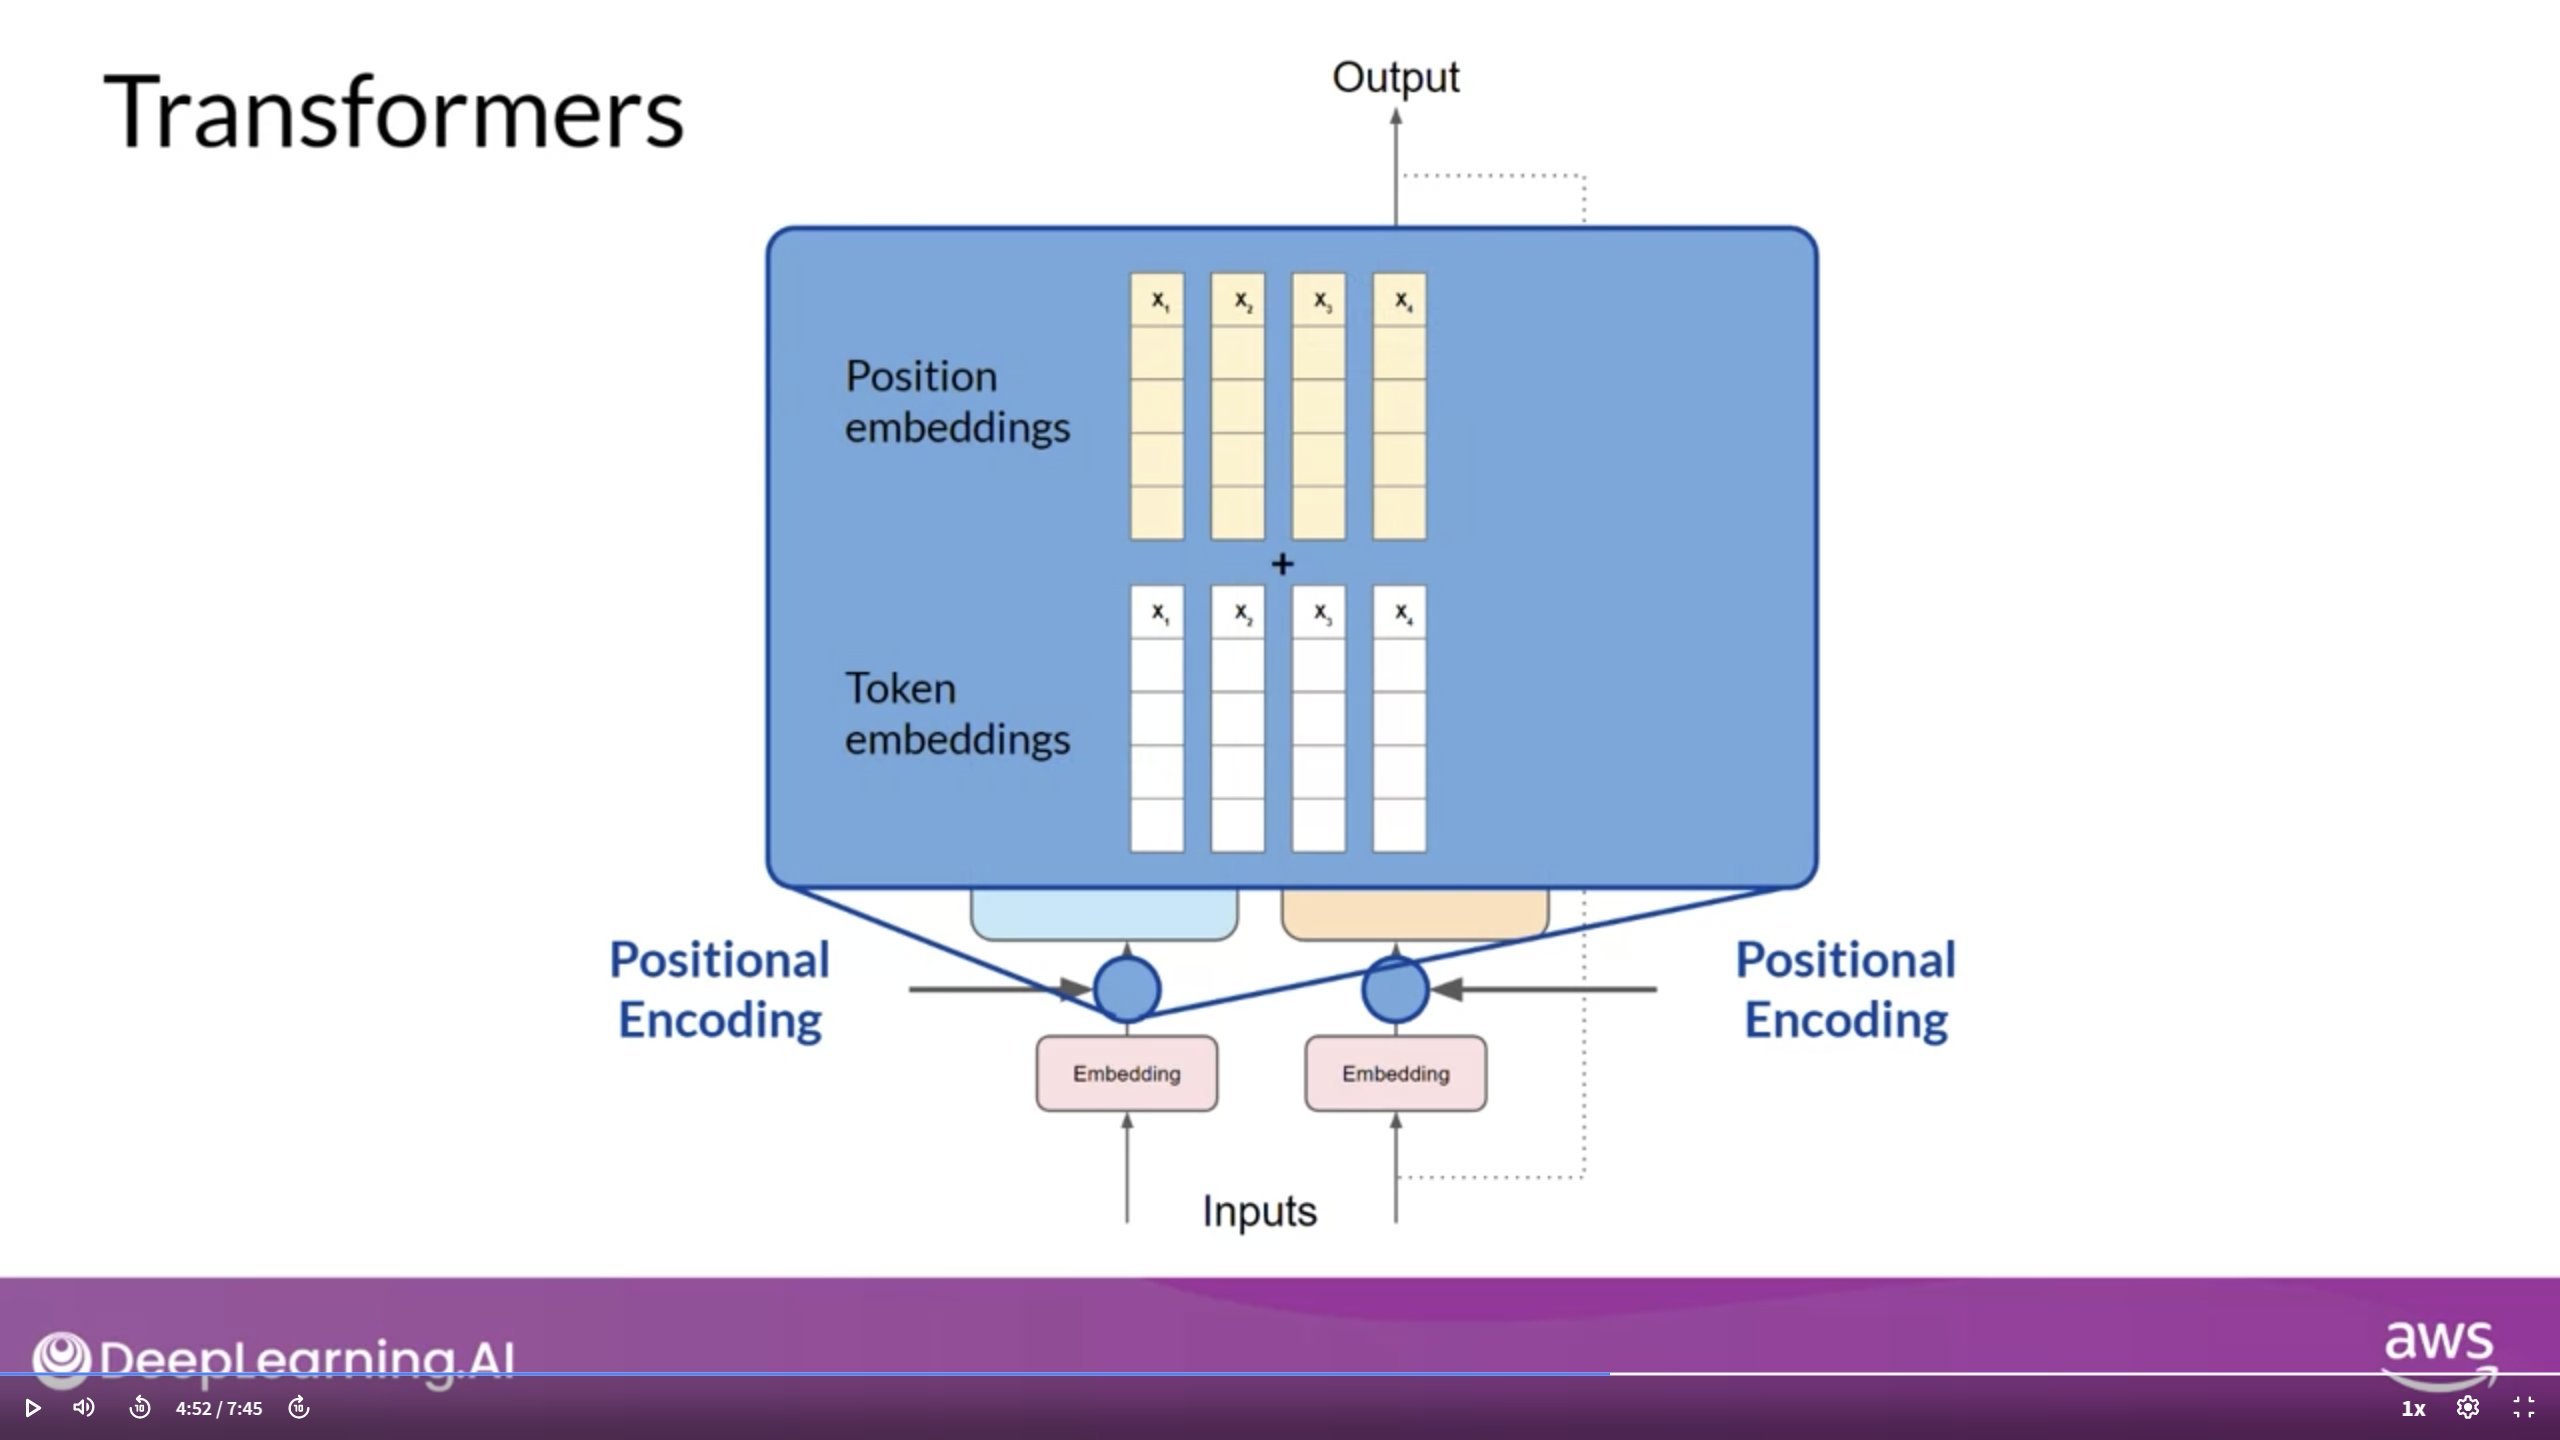
\includegraphics[trim=3cm 7cm 5cm 0cm,clip,scale=0.15]{pics/positional.png}
  %{\footnotesize\textbf{Notes:} XXX.} % changed <<<<<<<<<<
  %#\label{XXX}
\end{figure}


Step 4: Self-attention layer. The model analyzes the relationships between the tokens in your input sequence. This allows the model to attend to different parts of the input sequence to better capture the contextual dependencies between the words. The self-attention weights  that are learned during training and stored in these layers reflect the importance of each word in that input sequence to all other words in the sequence.


Step 5: Multi-headed self-attention. Multiple sets of self-attention weights or heads are learned in parallel independently of each other,. The number of attention heads included in the attention layer varies from model to model, but number in the range 12~100 are common. Each self-attention head will learn a different aspect of language. For example, one head may see the relationship between the people entities in our sentence. Whilst another head may focus on the activity of the sentence. Another head, may search for other properties. The weights of each head are randomly initialized, so each, randomly, learn different aspect of the language.


\begin{figure}[H]
  \centering
  \caption{Multi-headed self-attention}
  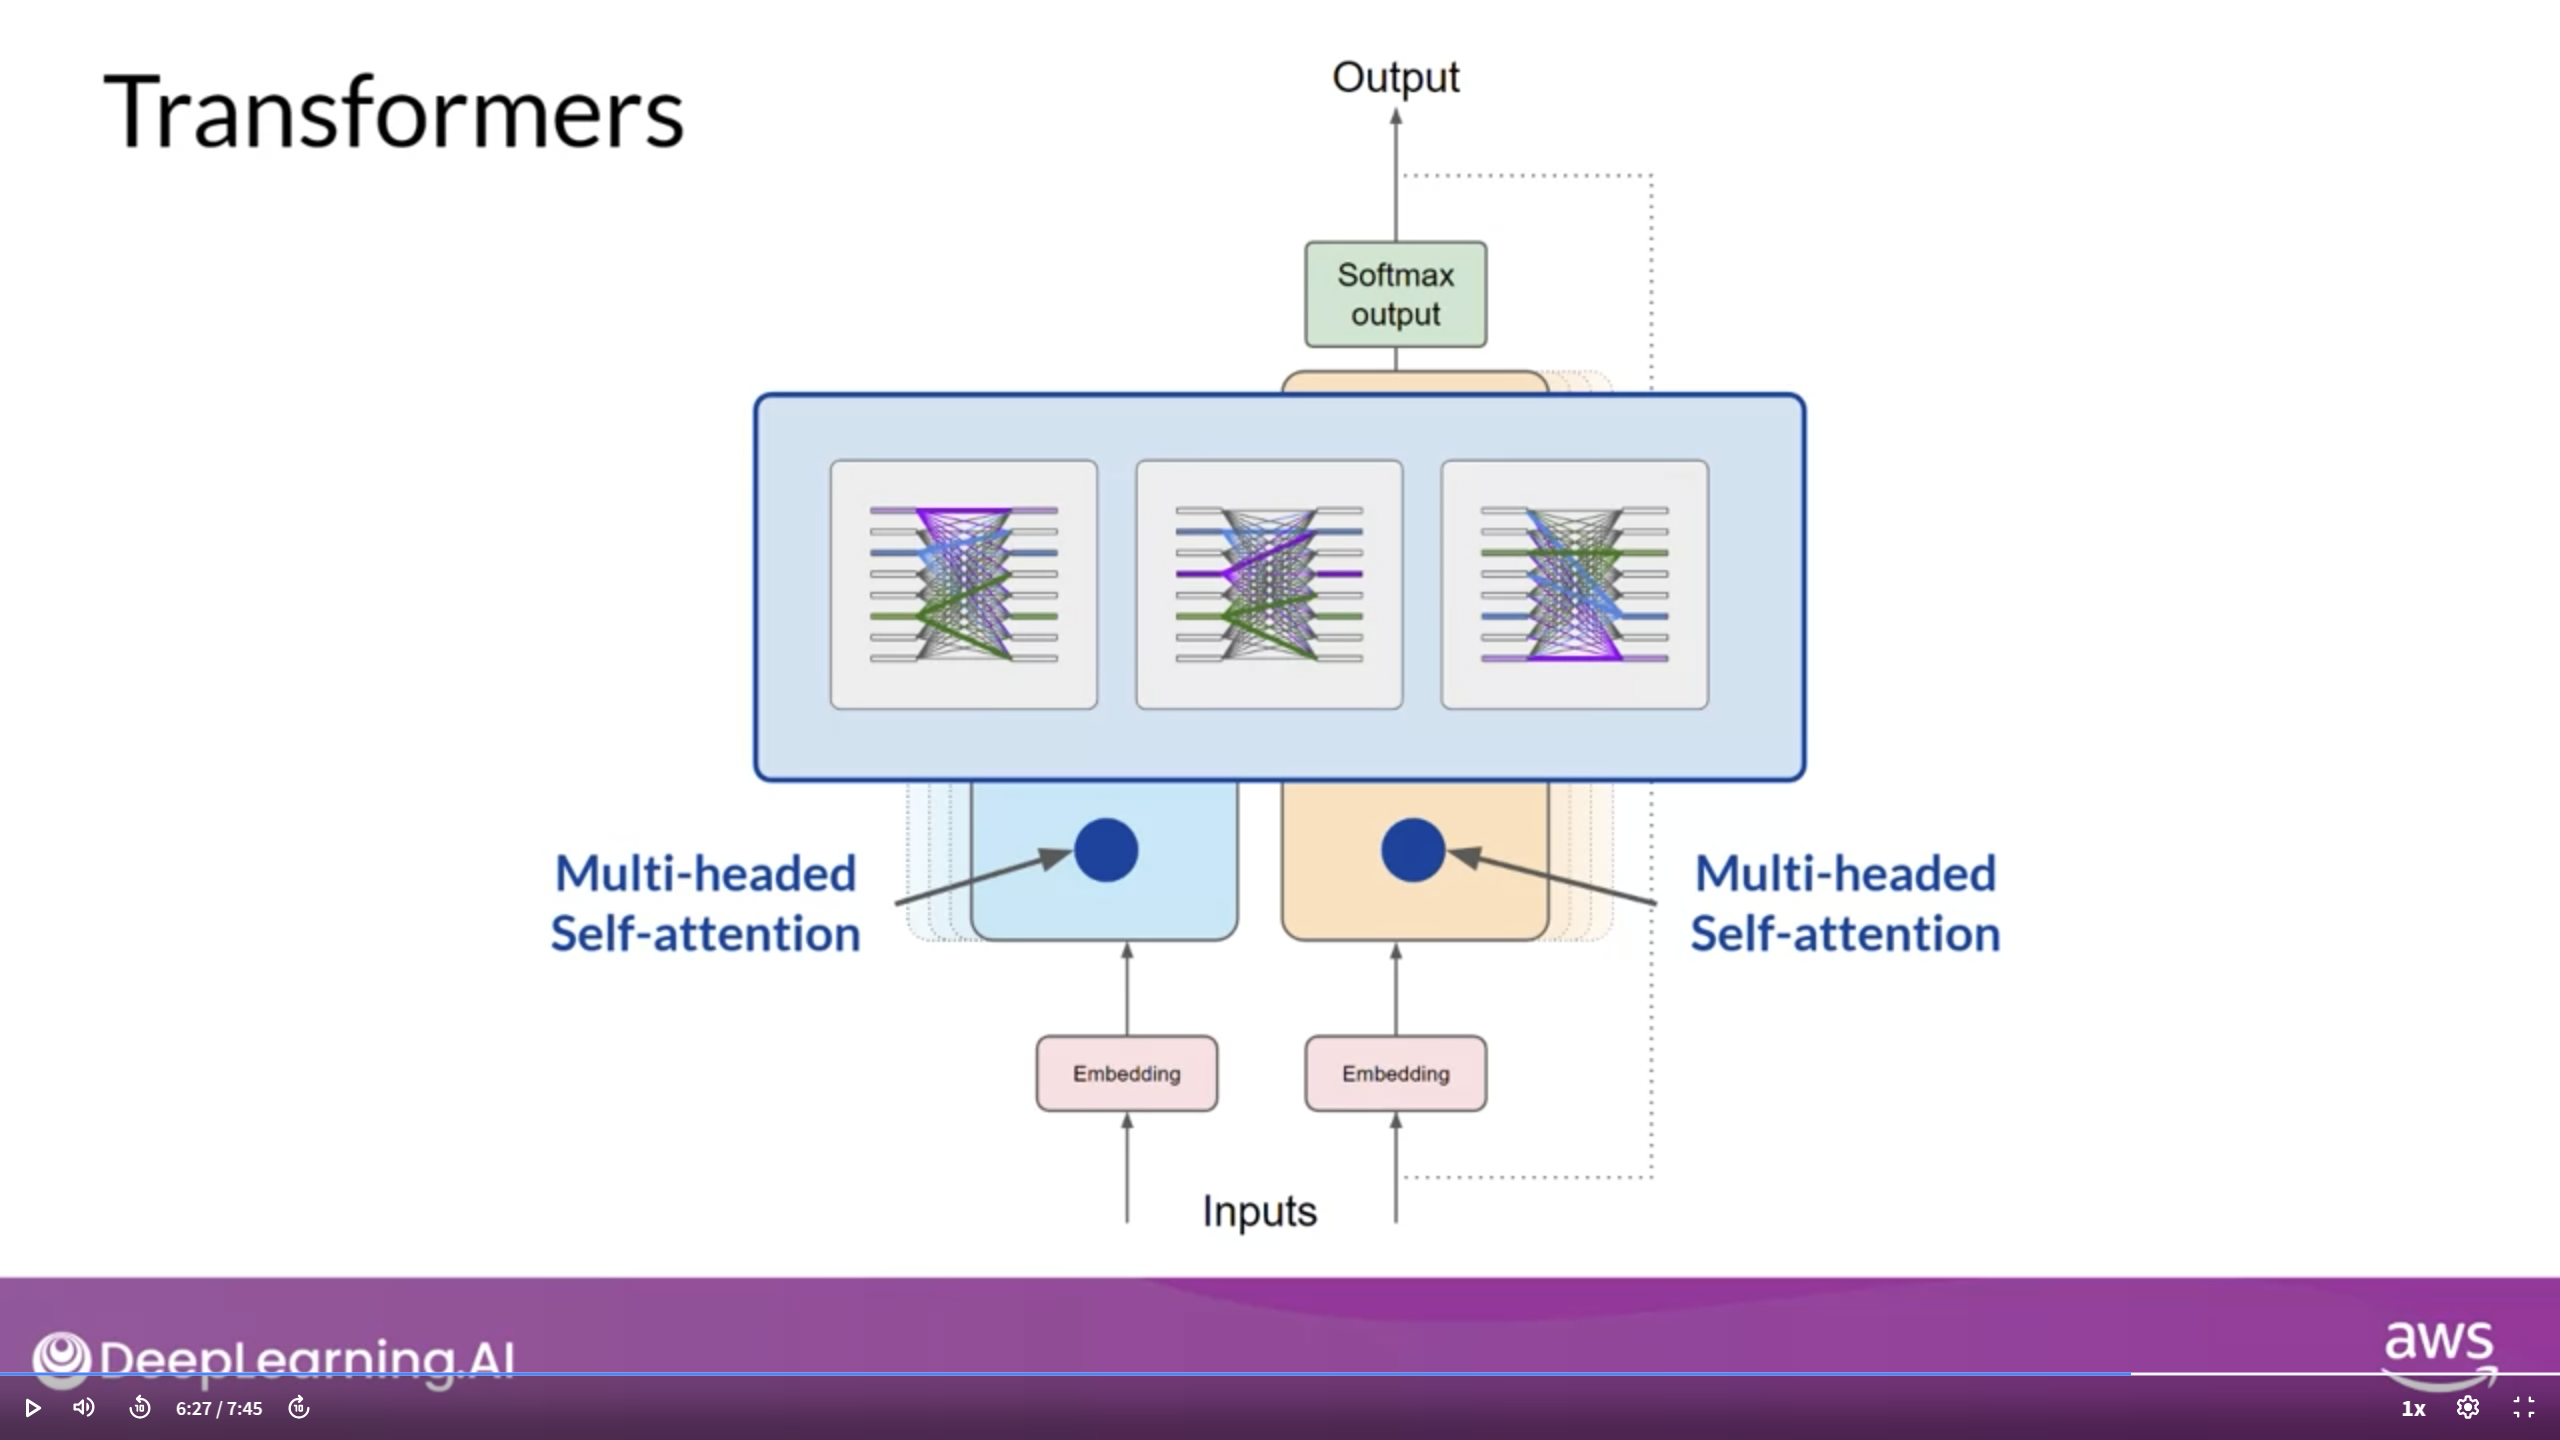
\includegraphics[trim=3cm 7cm 5cm 0cm,clip,scale=0.15]{pics/multiheaded.png}
  %{\footnotesize\textbf{Notes:} XXX.} % changed <<<<<<<<<<
  %#\label{XXX}
\end{figure}

Step 6: The output is processed through a fully connected feed forward network. The output of this layer is a vector of logics proportional to the probability score for each and every token in the tokenizer dictionary. You can pass these logics to the final softmax layer, where  they are normalized into a probability score for each word. This output includes a probability for every single word in the vocabulary, so there is likely to be thousands of scores here. One single token will have a score higher than the rest. This is the most likely predicted token. There are a number of methods that you can use to vary the final selection from this vector of probabilities.


\begin{figure}[H]
  \centering
  \caption{Feed forward network}
  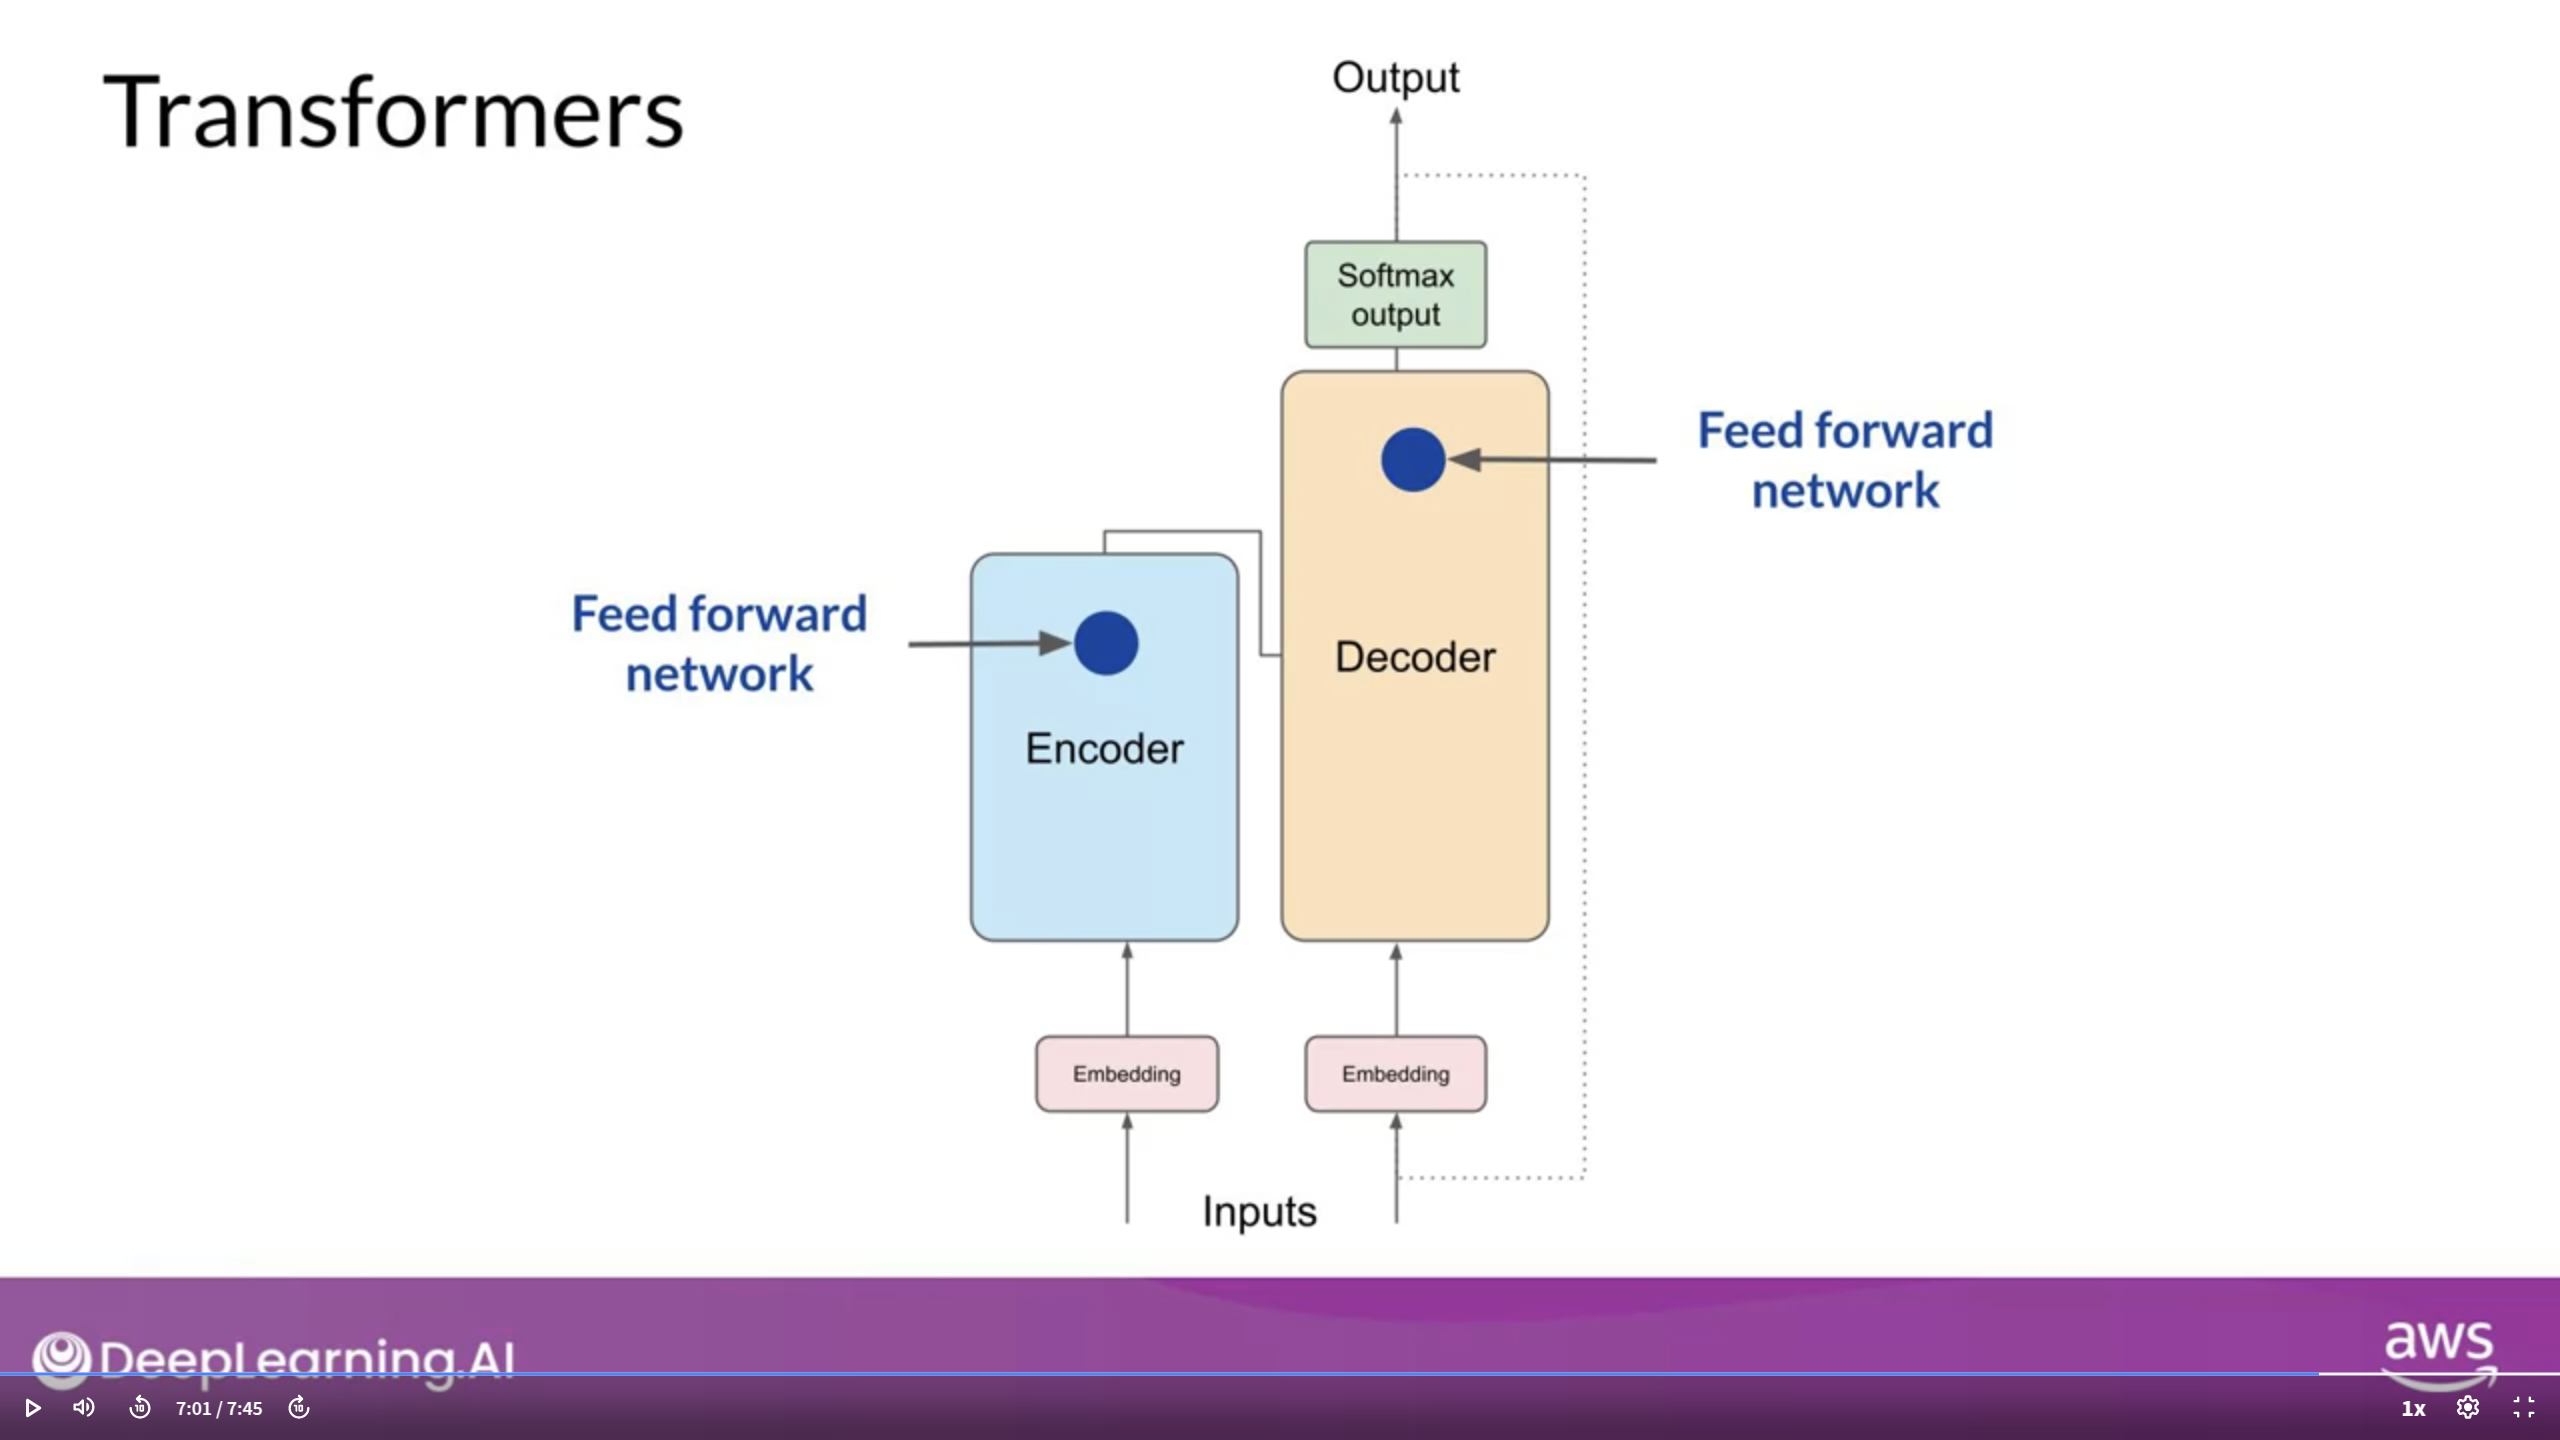
\includegraphics[trim=3cm 7cm 5cm 0cm,clip,scale=0.15]{pics/feed.png}
  %{\footnotesize\textbf{Notes:} XXX.} % changed <<<<<<<<<<
  %#\label{XXX}
\end{figure}

The process is depicted in the following picture, the process is iterative, until the end of the process, then, the final sequence of tokens are detokenized into words and you get the output


\begin{figure}
  \centering
  \begin{subfigure}[] %{.5\textwidth}
    \centering
    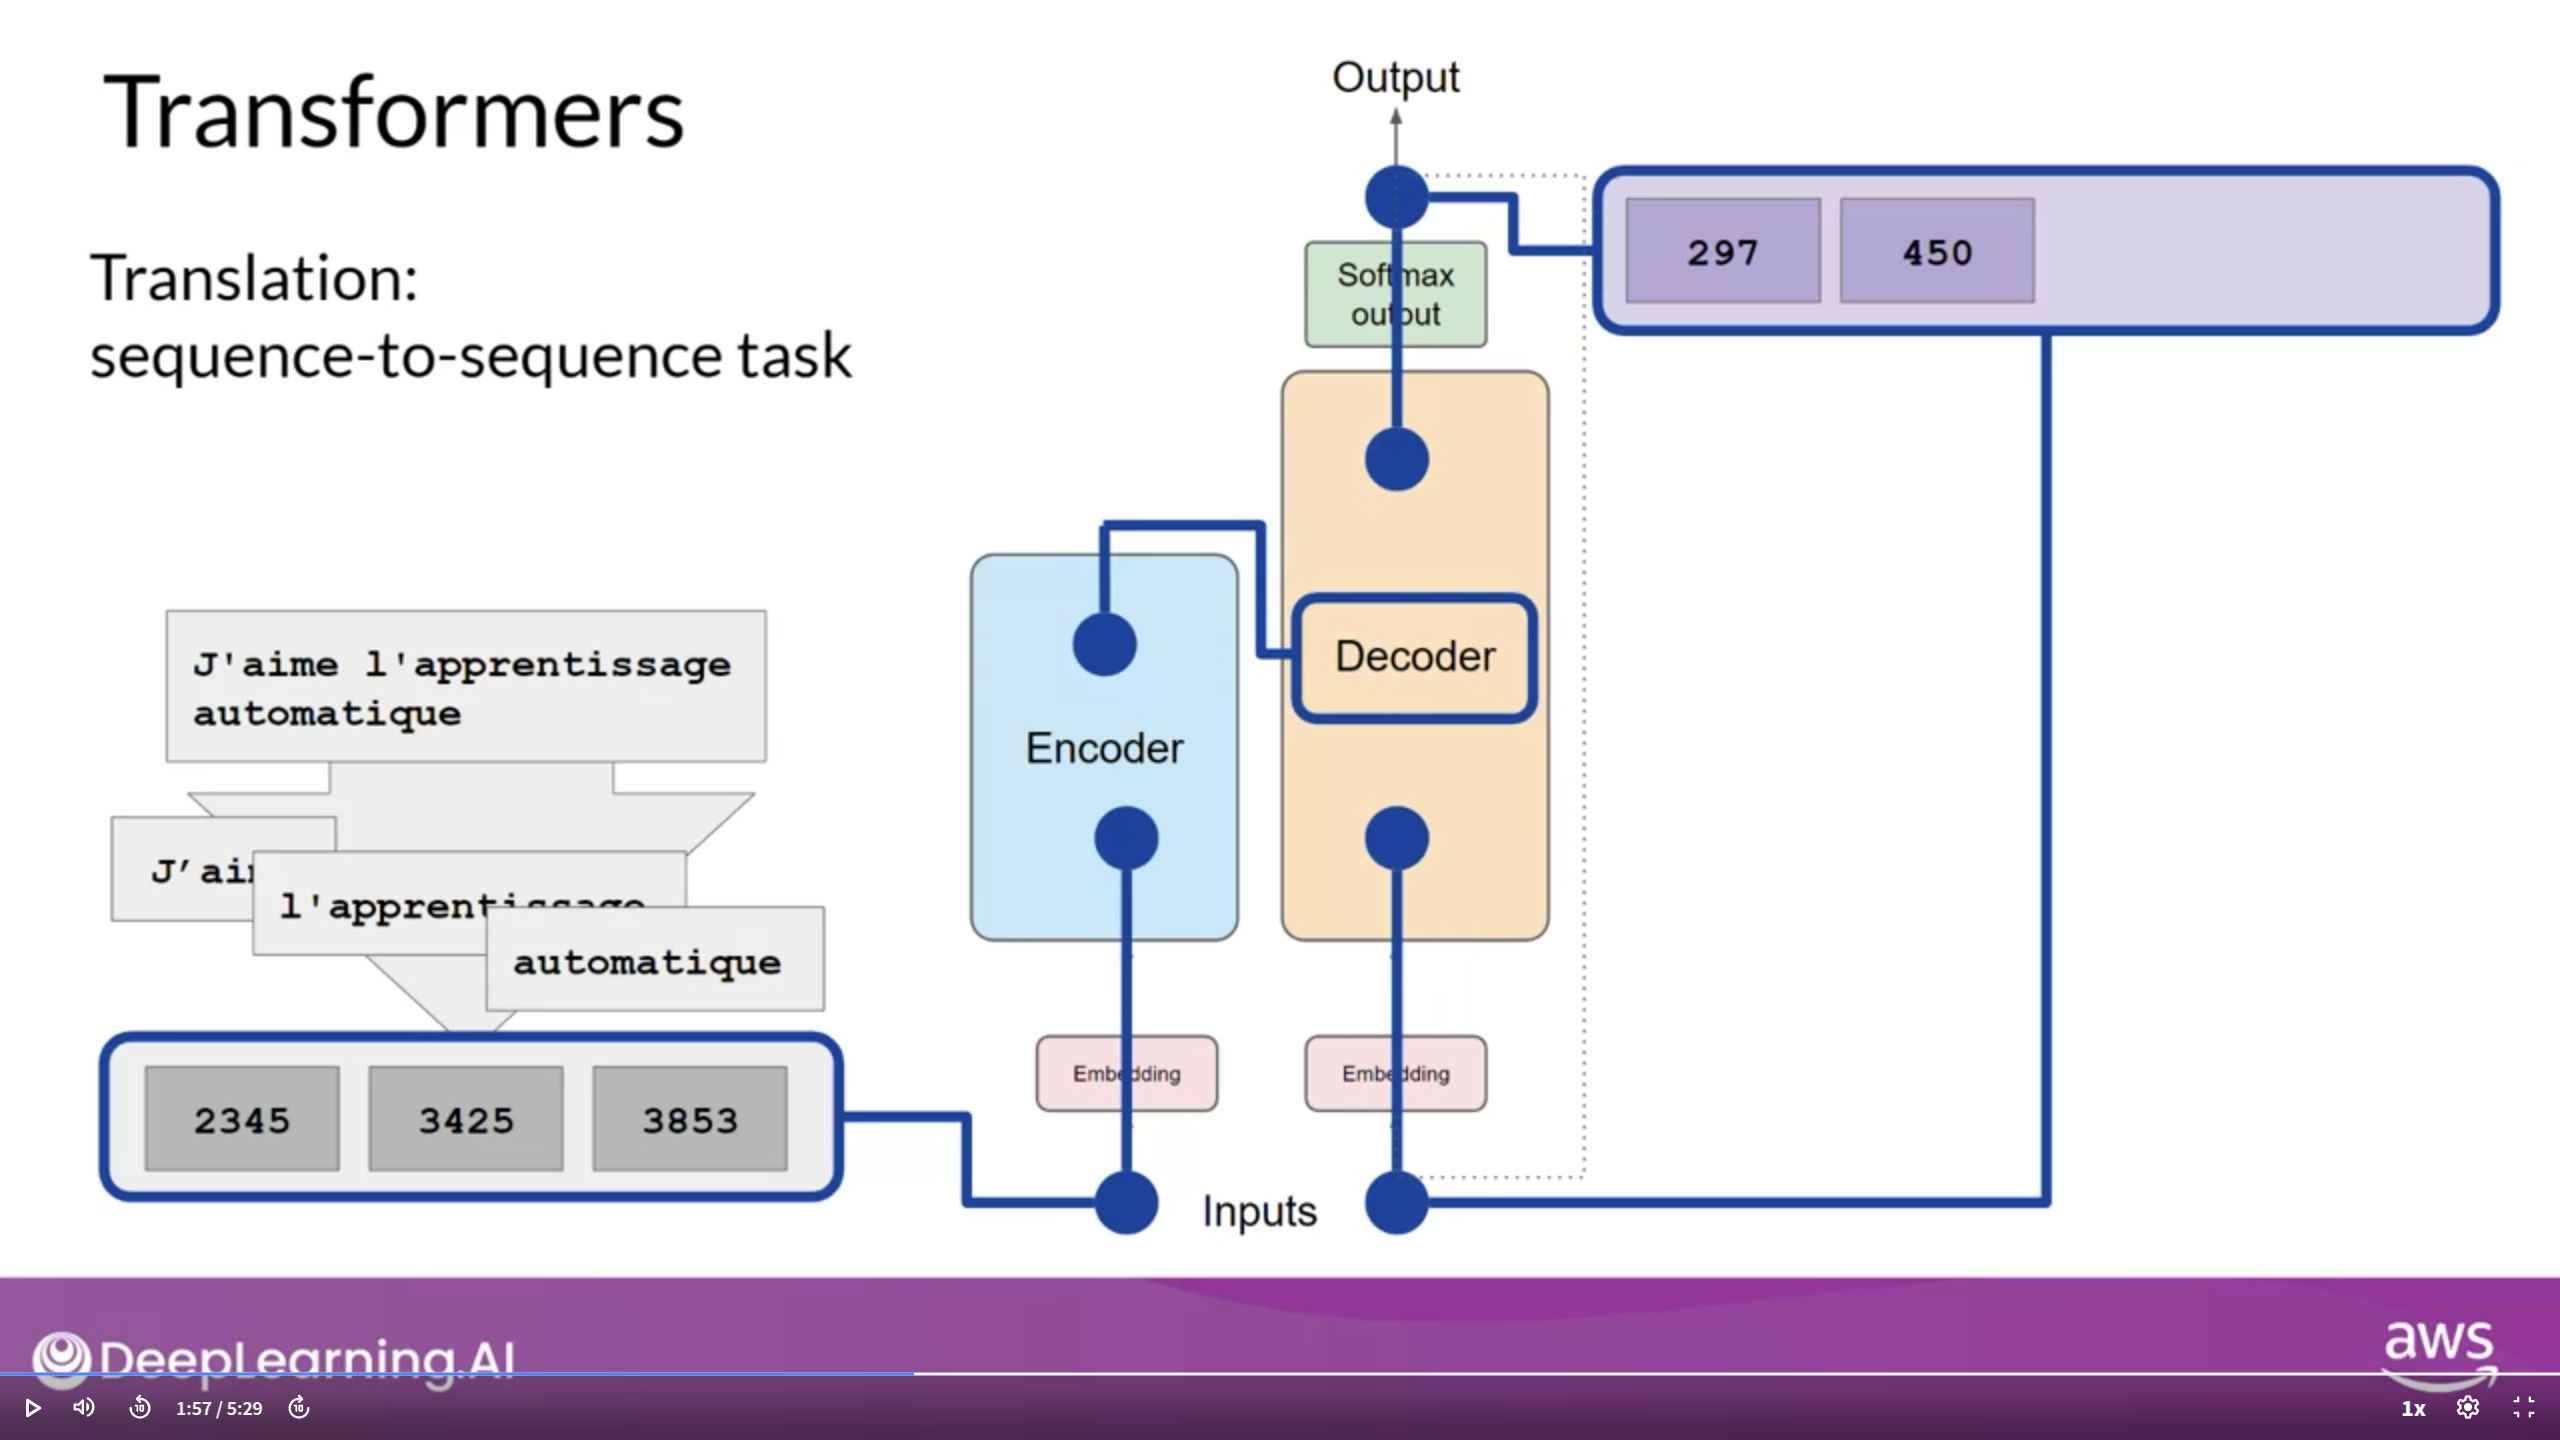
\includegraphics[scale=0.08]{pics/fullTransformer.png}
    %\caption{}
    %\label{fig:sub1}
  \end{subfigure}%
  \begin{subfigure}[] % {.5\textwidth}
    \centering
    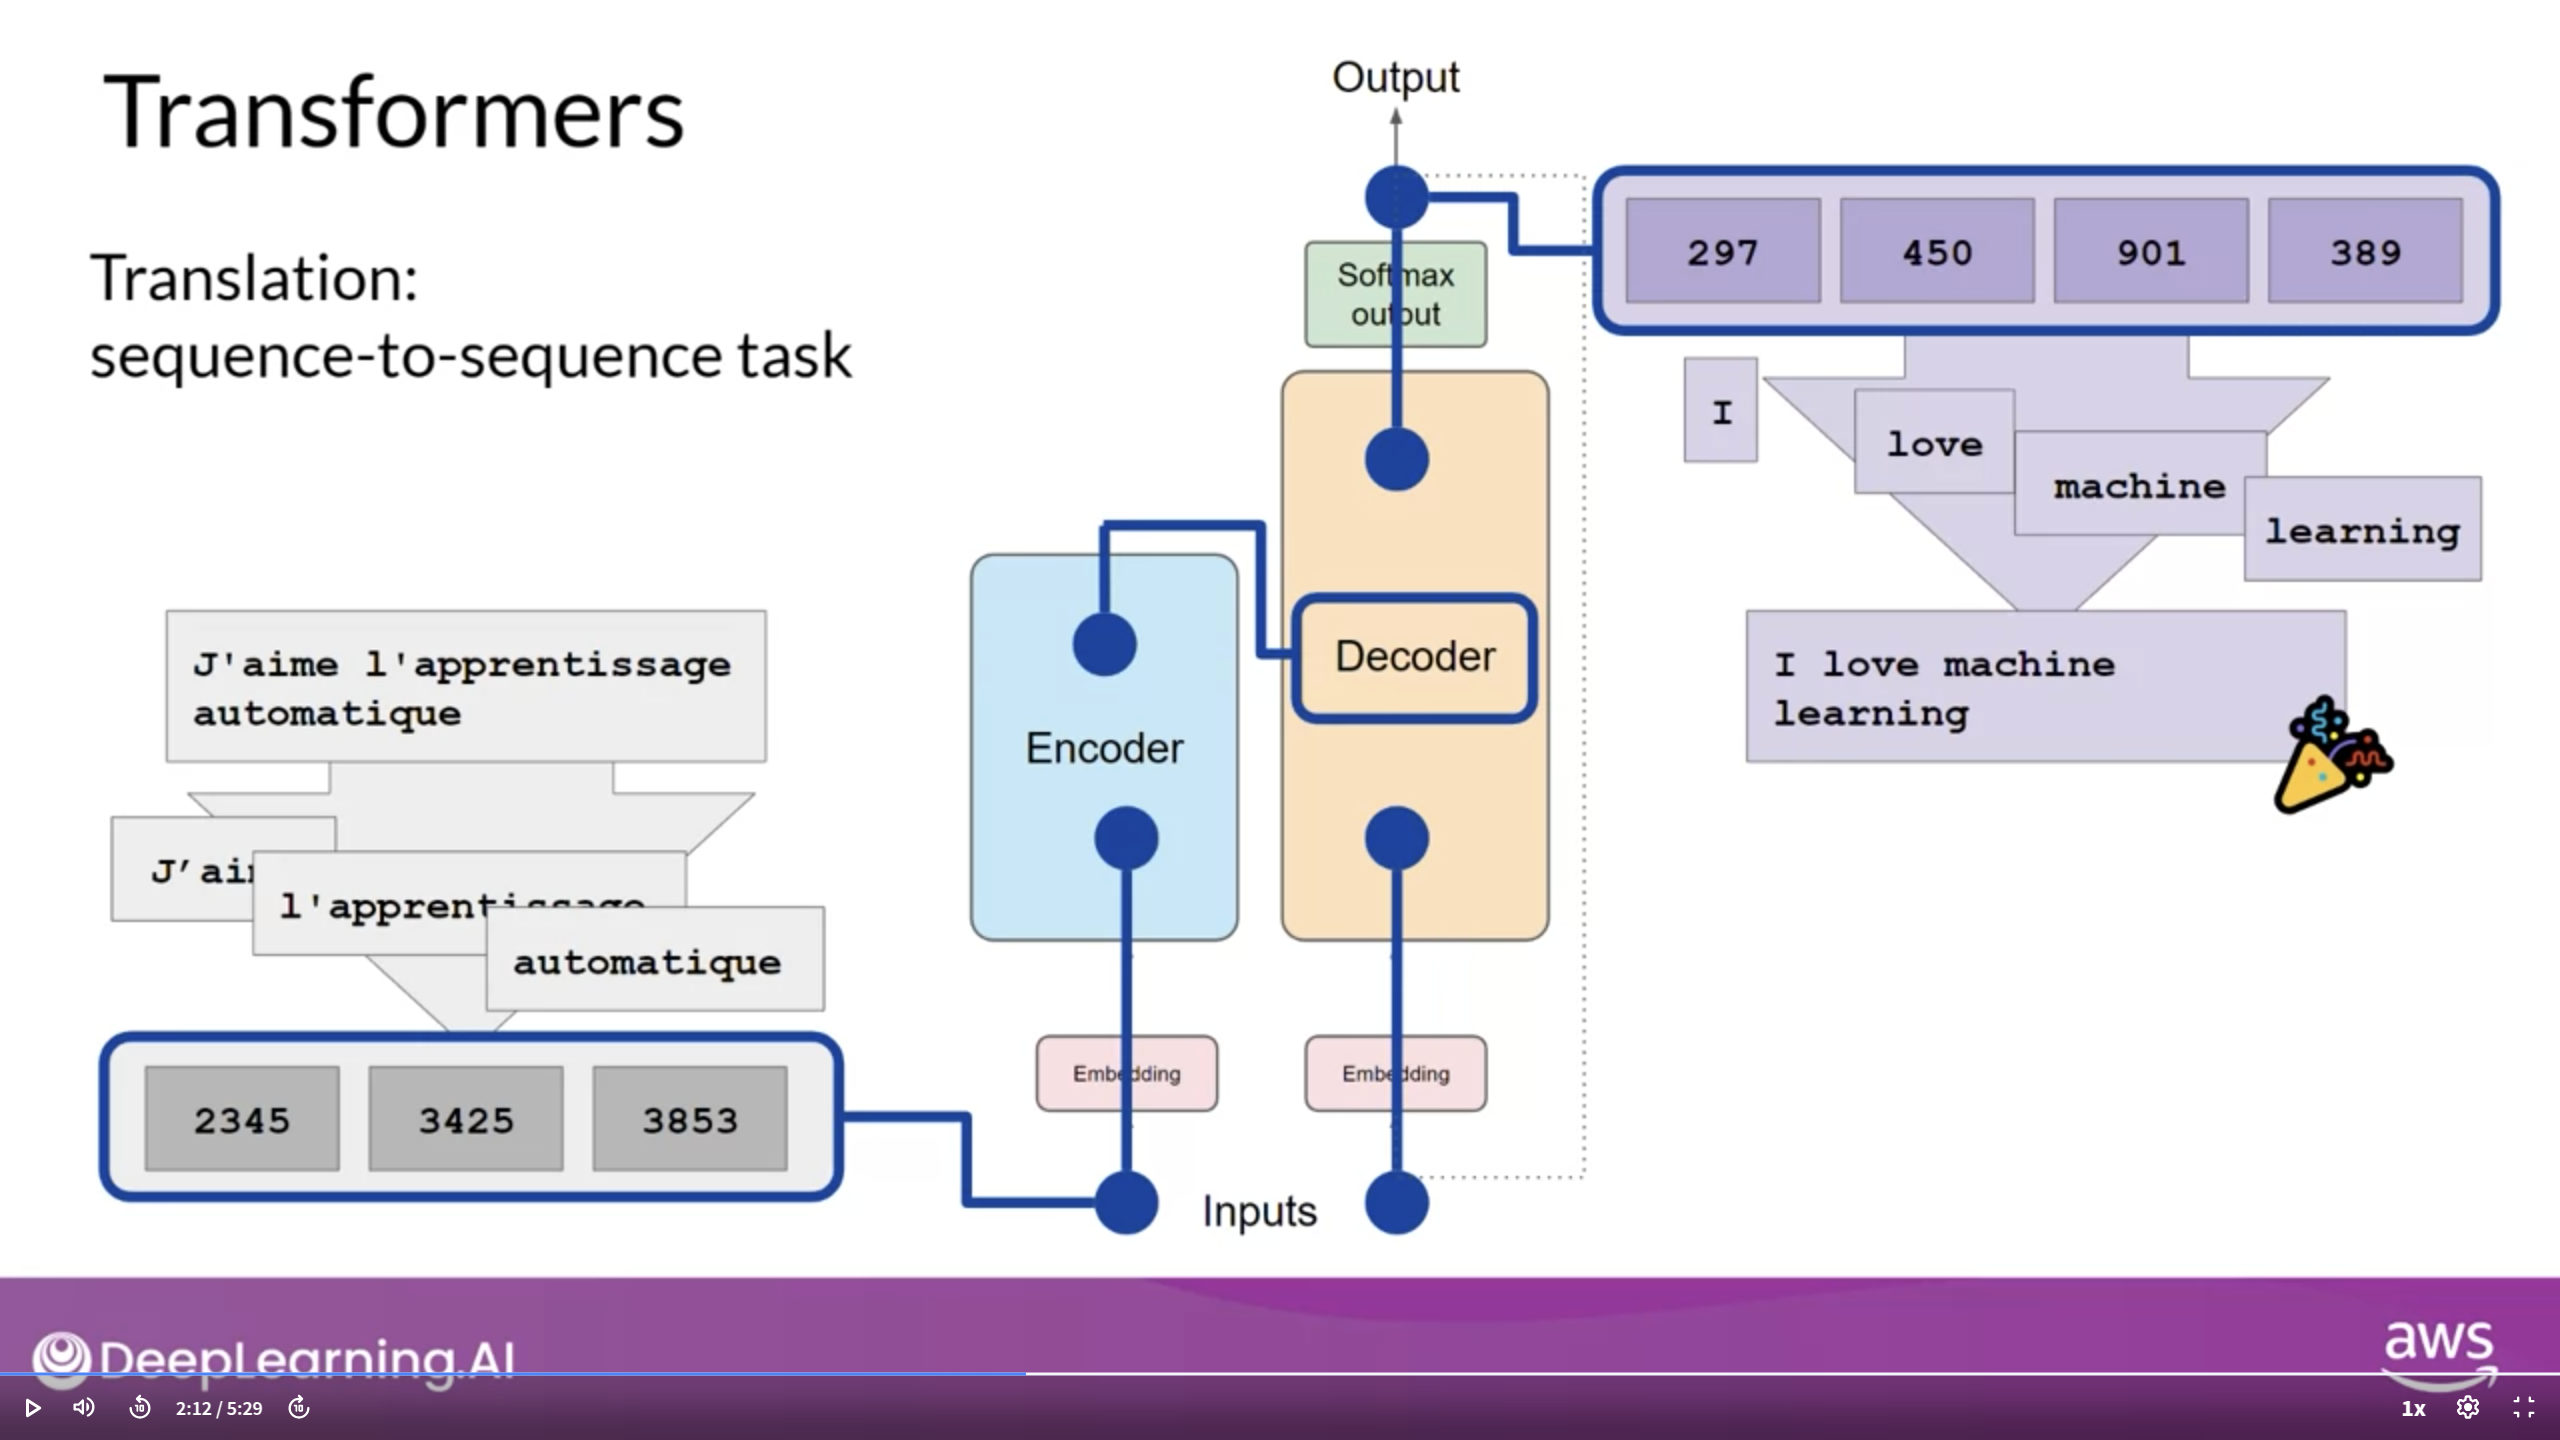
\includegraphics[scale=0.08]{pics/fullTransformer2.png}
    %\caption{}
    %\label{fig:sub2}
  \end{subfigure}
  \caption{Full transformer process: (a) Iterations of transformer model, (b) Detokenization of the final sequence}
  \label{fig:test}
\end{figure}


\section{Transformer types}
There are three different transformer models (see the picture below).

Some models only uses the Encoder section of the transformer (Encoder Only Models, AKA autoencoding models) by adding some extra layers to the output. These models are trained used Masked Language Modeling (MLM), which randomly masks some tokens from the sentence, and tries to guess the masked token. The model is bidirectional (from the beginning to end and end to the beginning of the sentence). These models are good for Sentiment analysis, Name entity recognition, and word classification. Famous autoencoding models are BERT and ROBERTA.

Decoder only models (autoregressive models) are trained using Causal Language Modeling (CLM). The training objective is to predict the next token based on the previous sequences of tokens (some researchers call this full language modeling). These models mask the input sequence and can only see the input tokens leading up to the token in question. The model has no knowledge of the end of the sentence and the context is unidirectional. These models are good for text generation, and other emergent behavior (depends on model size). Examples of these models are GPT, BLOOM, and LLaMa.

The third type of transformer models are Encoder/Decoder or sequence-to-sequence models. It masks a f few words from the sentence, combines it into one token, then it tries to predict the masked tokens (which is also called sentinel token). These models are good for translation, text summarization, and question answering. BART and T5 are of this type.


\begin{figure}[H]
  \centering
  \caption{Different transformer models}
  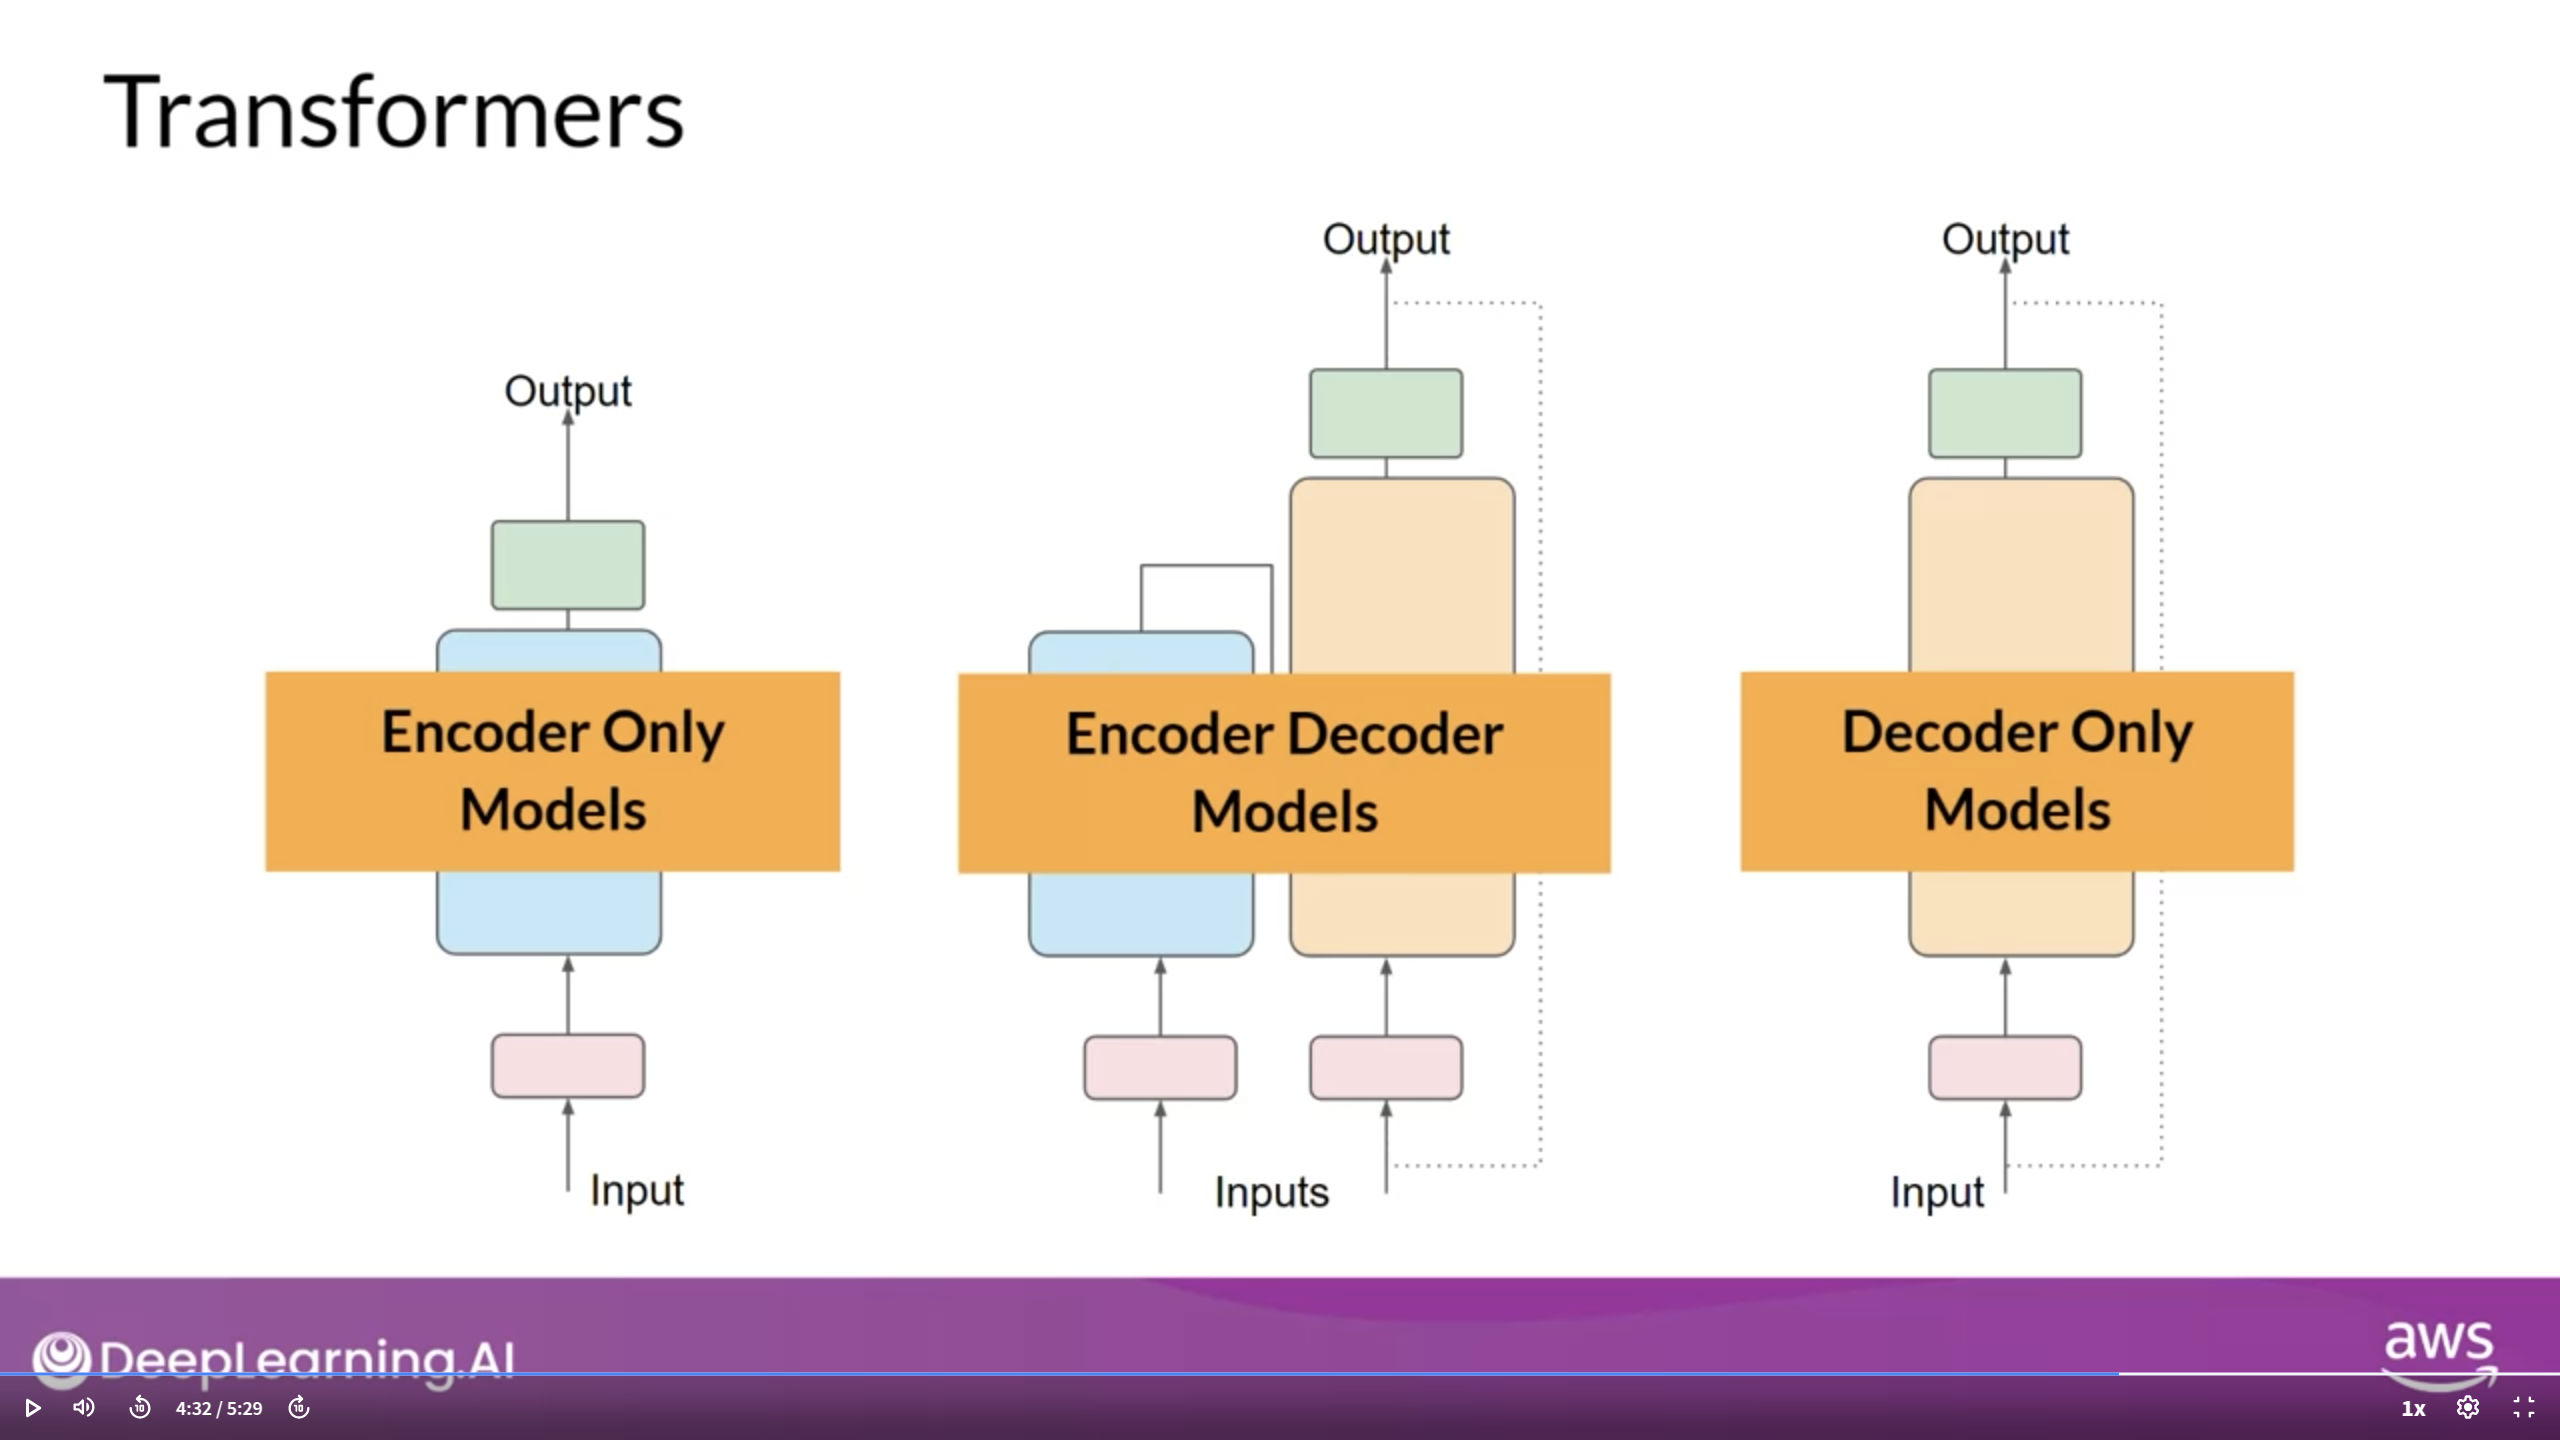
\includegraphics[trim=3cm 7cm 5cm 0cm,clip,scale=0.15]{pics/VariousTransformers.png}
  %{\footnotesize\textbf{Notes:} XXX.} % changed <<<<<<<<<<
  %#\label{XXX}
\end{figure}


Model architectures and pre-training objectives of these three types of transformers are depicted in the next picture.

\begin{figure}[H]
  \centering
  \caption{Pretraining objective of each transformer types}
  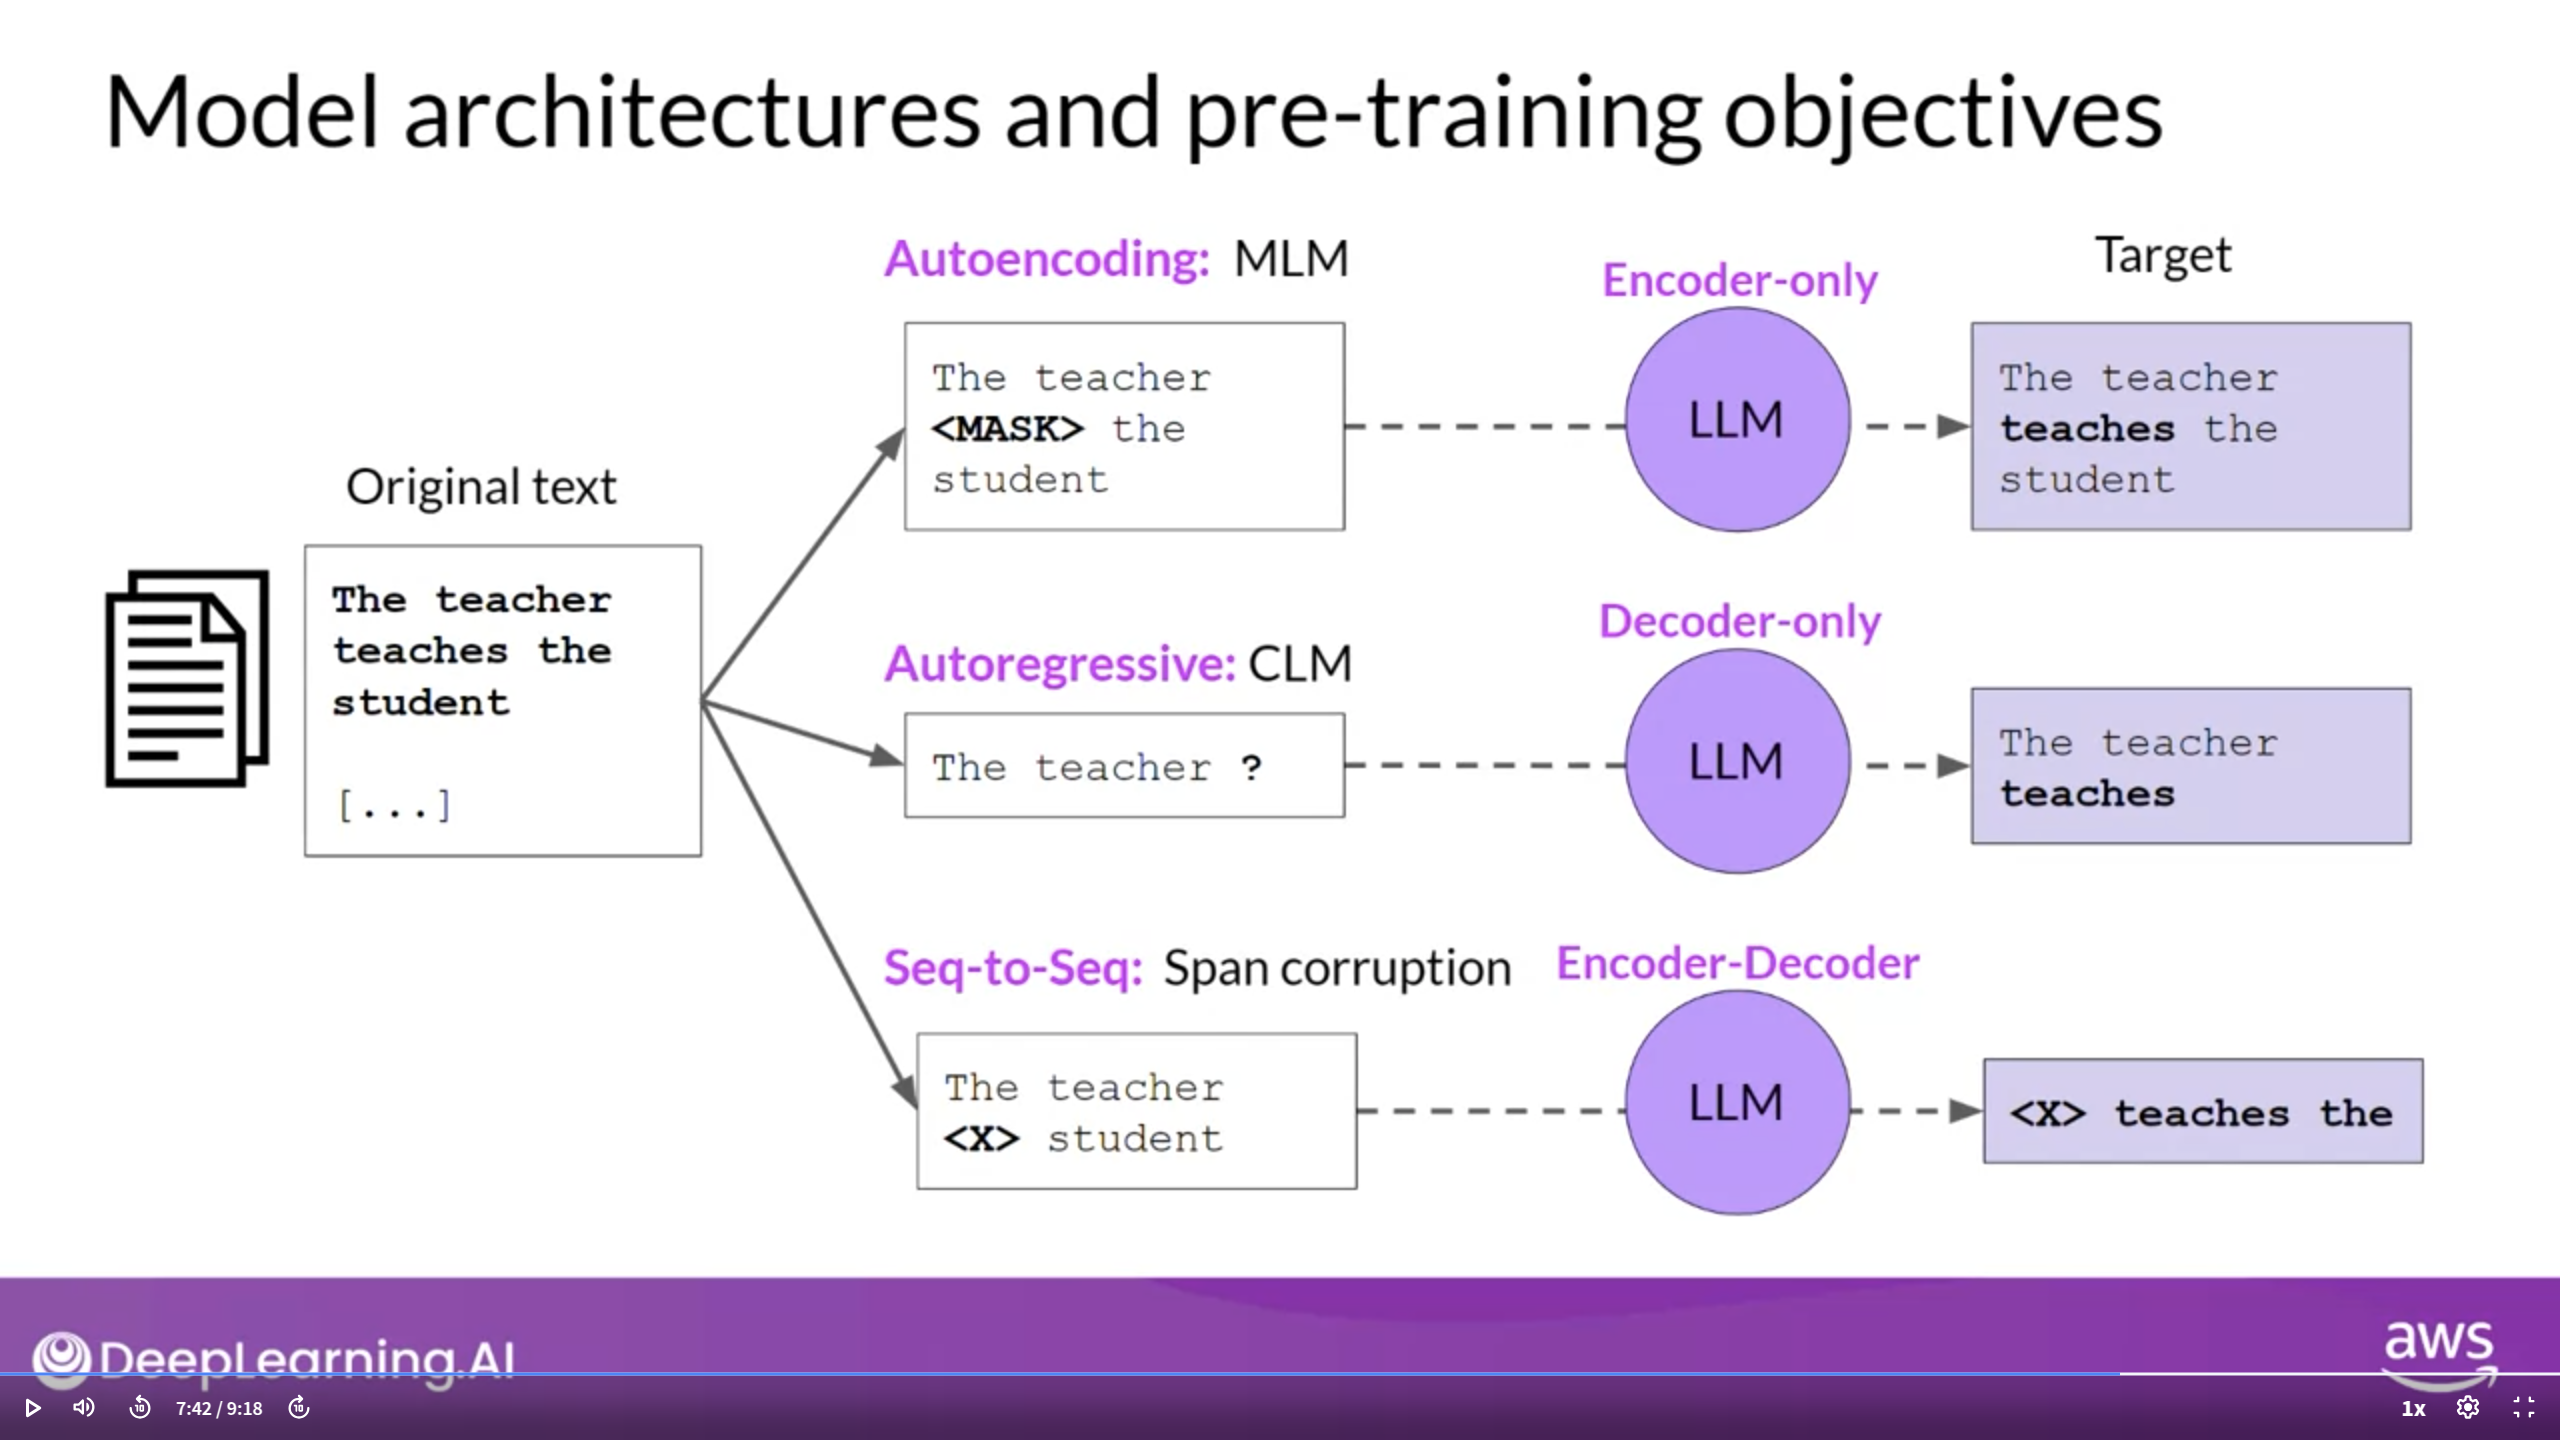
\includegraphics[trim=3cm 7cm 5cm 0cm,clip,scale=0.15]{pics/pretraining.png}
  %{\footnotesize\textbf{Notes:} XXX.} % changed <<<<<<<<<<
  %#\label{XXX}
\end{figure}



Issues of transformers: Hallucinations are words or phrases that are generated by the model that are often nonsensical or grammatically incorrect. This may cause by a number of factors: when a model is not trained on enough data, trained on noisy or dirty data, not given enough context, not given enough constraints.

\section{Prompt engineering}
A prompt is a short piece of text that is given to a large language model or LLM, as input, and it can be used to control the output of the model in a variety of ways. Prompt design is the process of creating a prompt that is tailored to the specific task that the system is being asked to perform. Prompt engineering is the process of creating a prompt that is designed to improve performance.


Different Gen AI model types: text-to-text (Ex: translation), text-to-image are trained on a large set of images, each captioned with a short text description, text-to-video, text-to-3D, and text-to-task.


There are three different Language models: Generic (or row) language models: predict the next word (technically, token) based on the language in the training data. Instruction tuned models: trained to predict a response to the instructions given in the input. Dialogue tuned models: trained to have a dialog by predicting the next response.


The more parameter a model has, the more memory it has, and the more sophisticated the task it can perform.

The text you pass to LLM is known as a prompt. The space you have for prompt is called the context window (usually 1000 words). The output of the model is called a completion. The act of using the model to generate an answer is called inference.

\begin{figure}[H]
  \centering
  \caption{Different transformer models}
  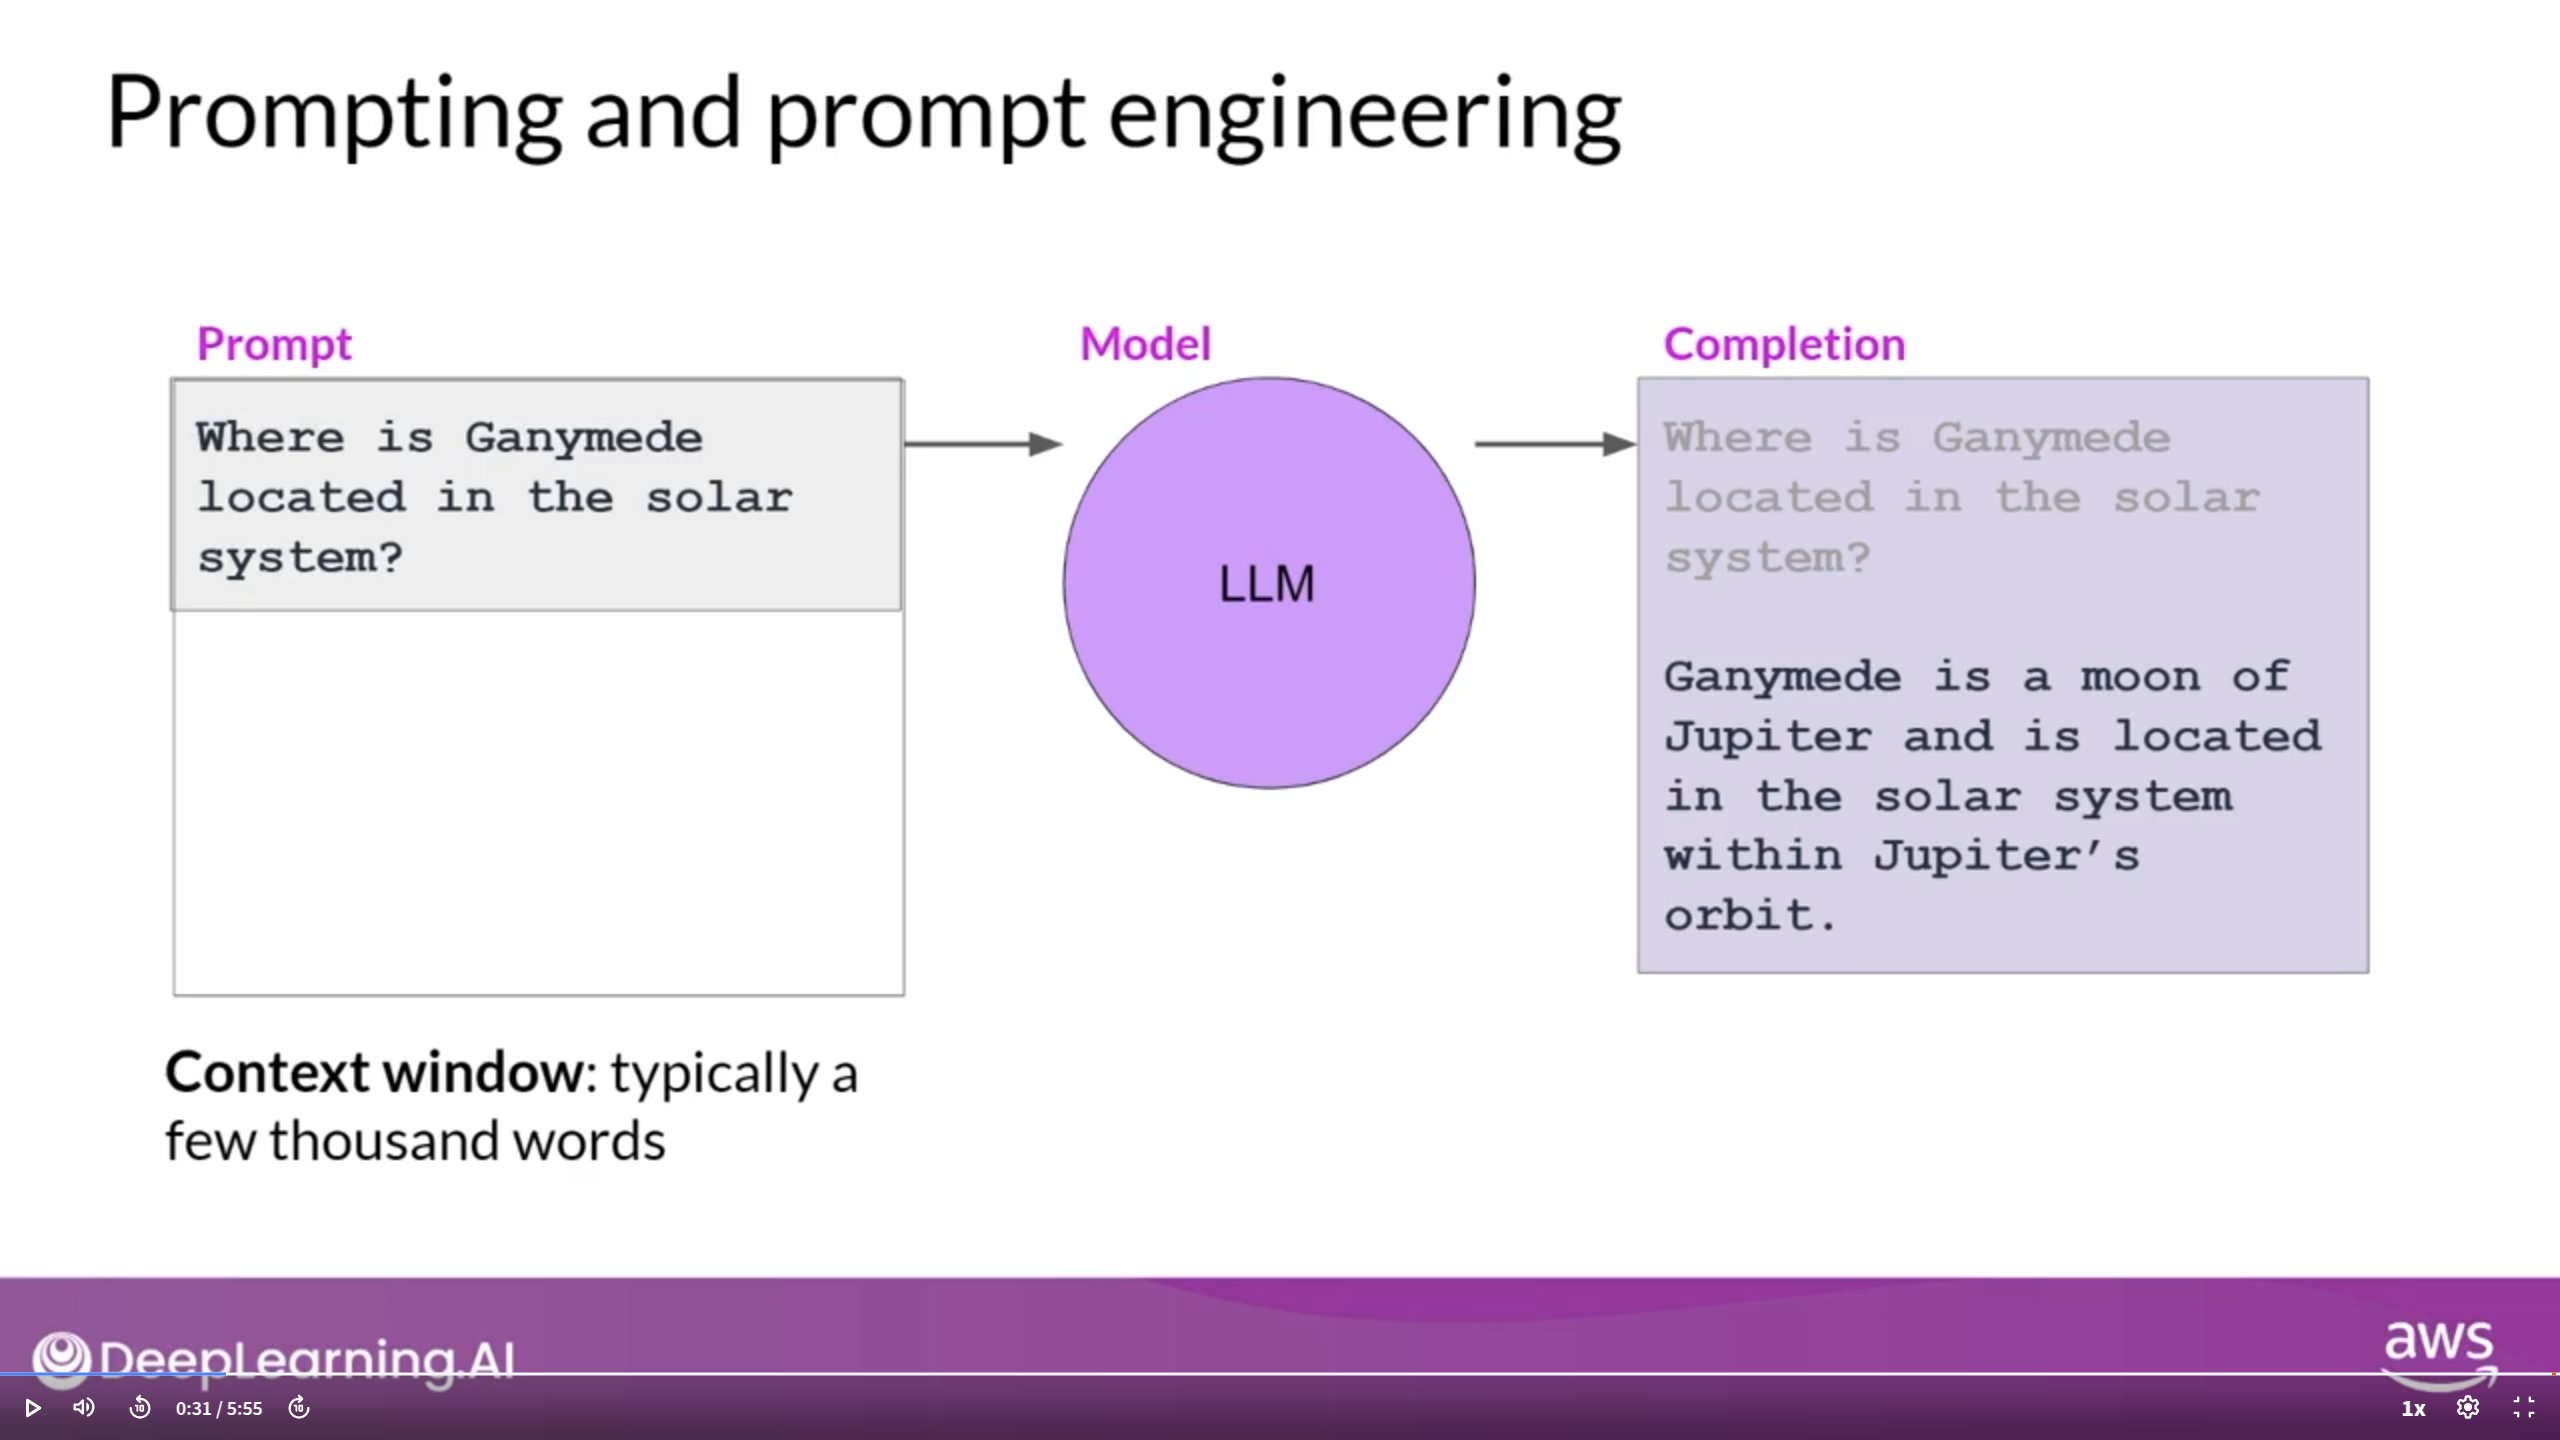
\includegraphics[trim=3cm 7cm 5cm 0cm,clip,scale=0.15]{pics/prompt.png}
  %{\footnotesize\textbf{Notes:} XXX.} % changed <<<<<<<<<<
  %#\label{XXX}
\end{figure}

We frequently encounter situations where the model does not produce the outcome you want, on the first try (Zero-shot inference). So, you may have to reviset the language in the prompt.The work to improve the prompt is known as prompt engineering. One way in prompt engineering is to provide examples in the prompt, which is known as in-context learning (ICL). See a one-shot inference in the picture below. We can extend the strategy to have few-shot inference. Sometimes, adding more shots, does not improve the output, for example, if you don't get better answers with 5 shot, probably does not worth try more shots. Also, you need to make sure that you do not exceed the model's input-context length. If the answer is not desirable even with few examples, we need to fine-tune the model.


\begin{figure}
  \centering
  \begin{subfigure}[] %{.5\textwidth}
    \centering
    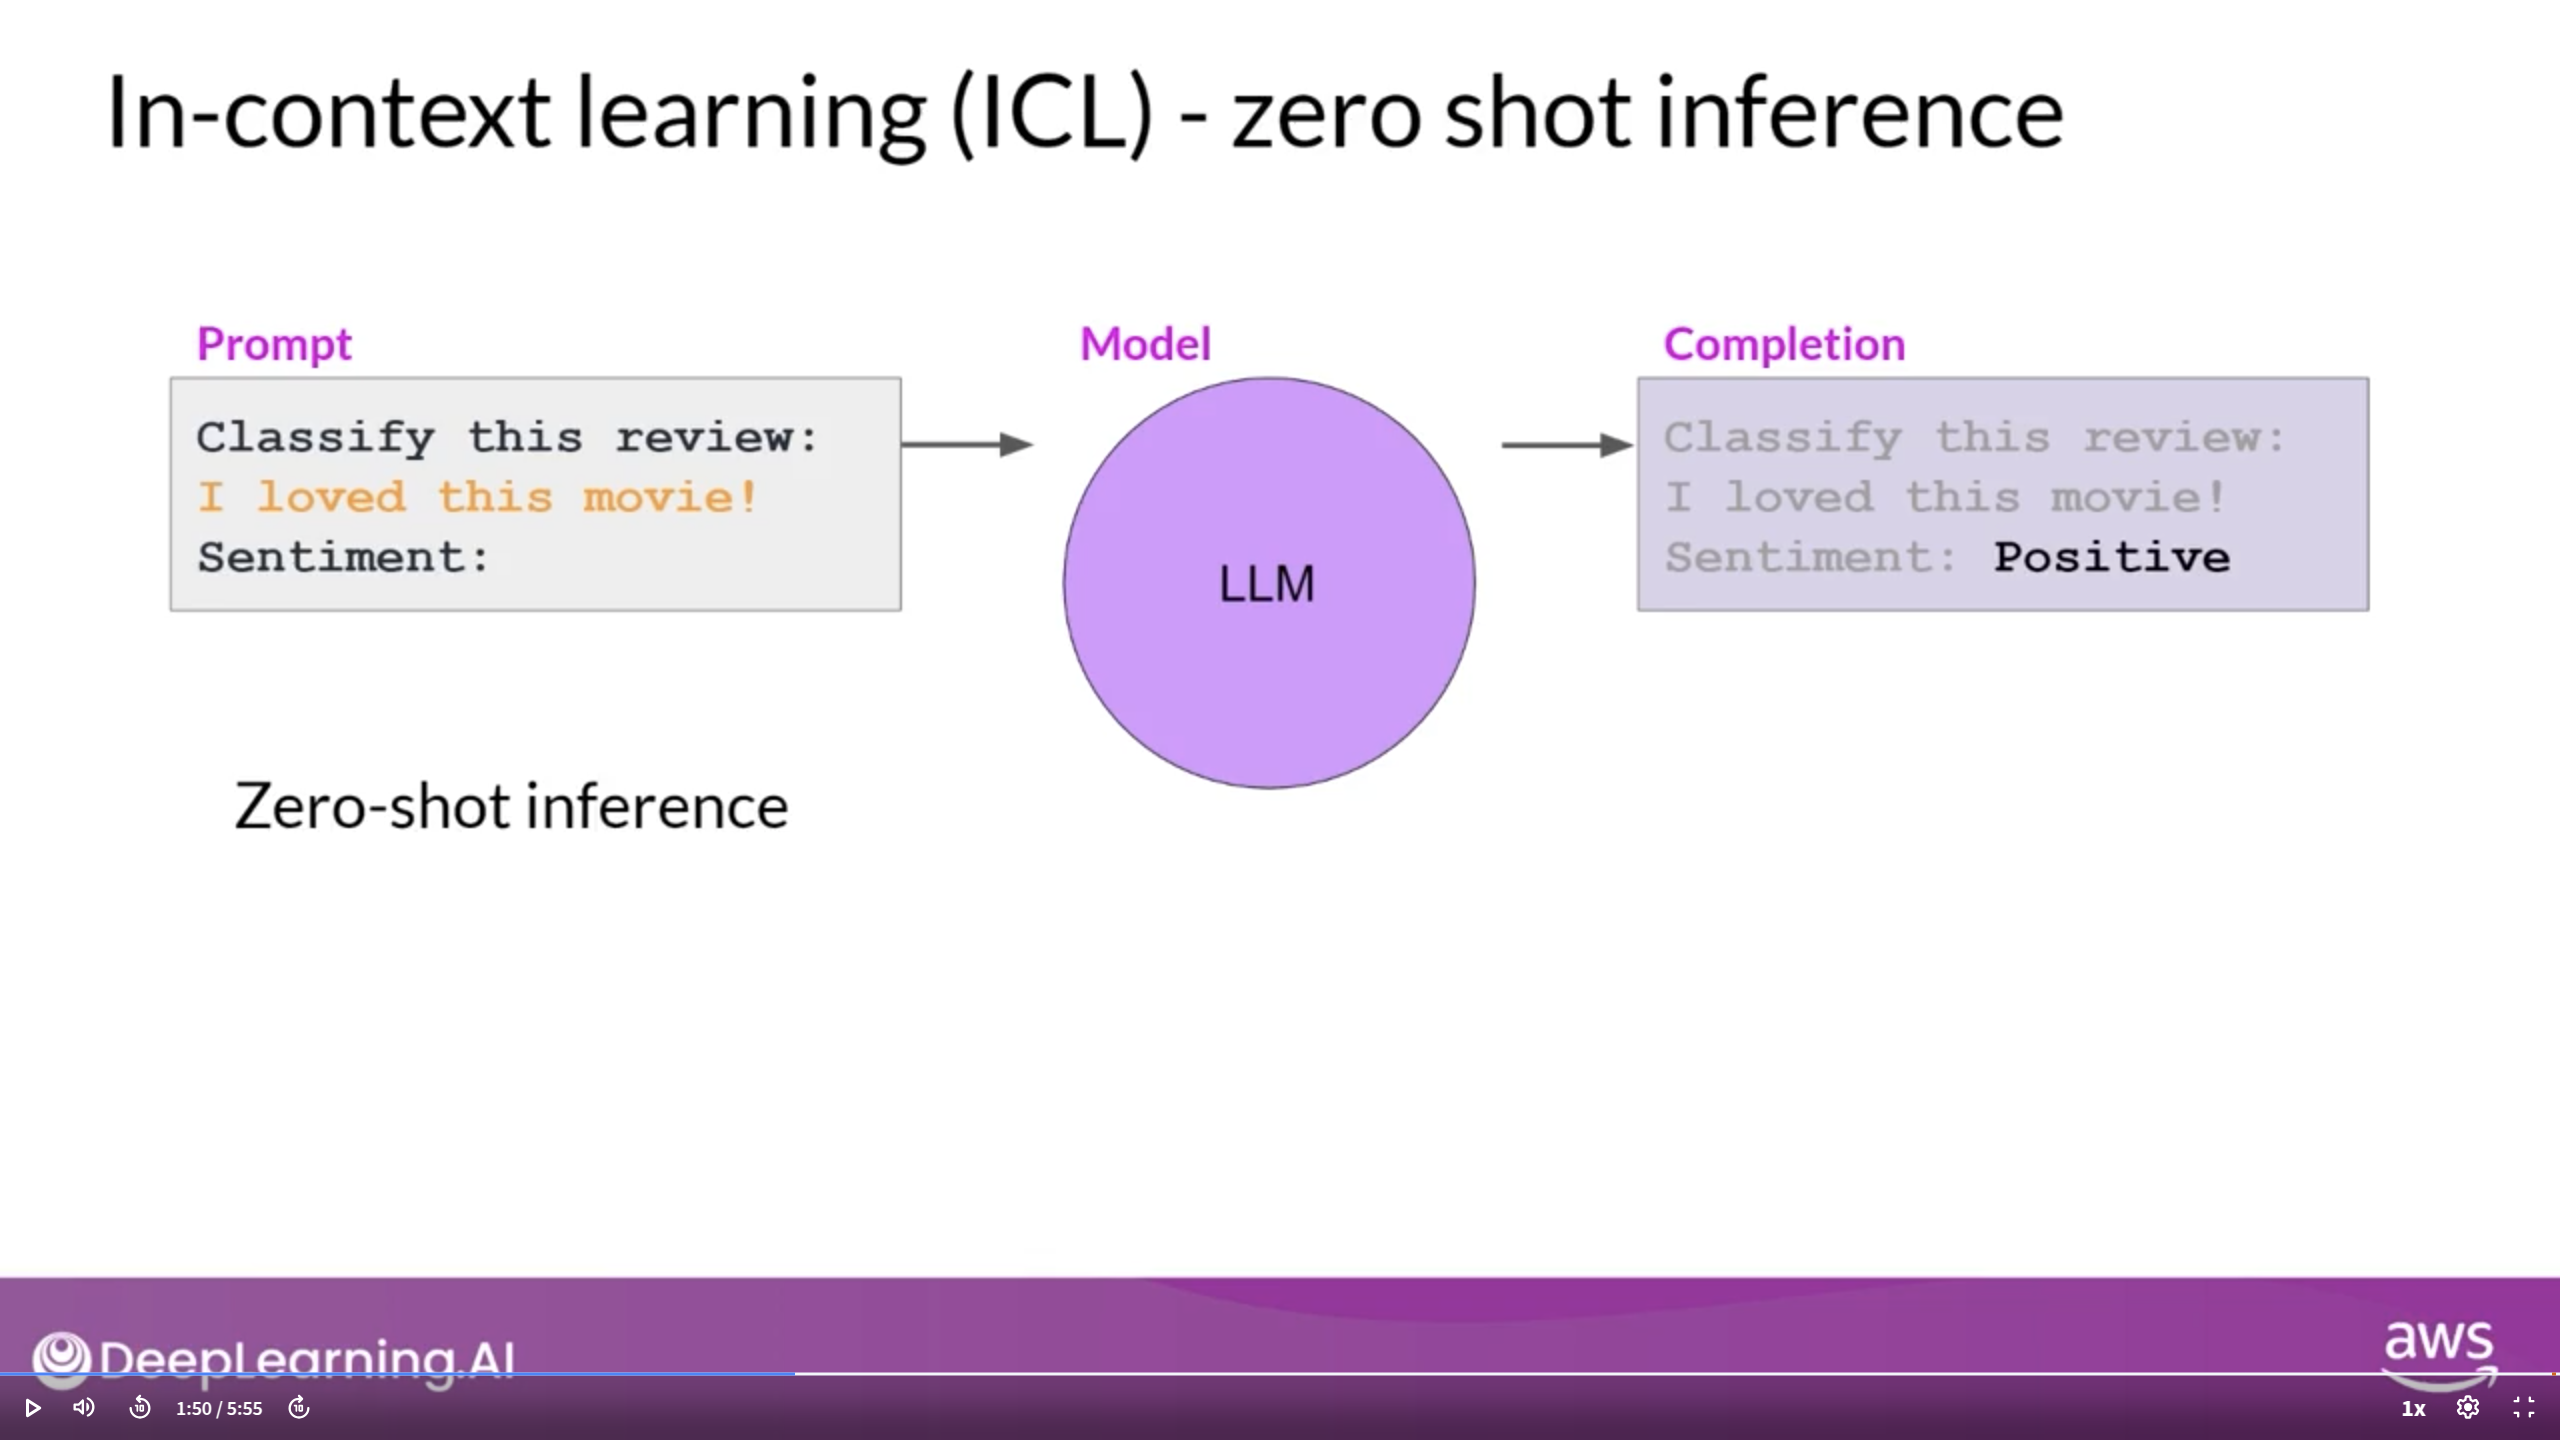
\includegraphics[trim=3cm 7cm 5cm 0cm,clip,scale=0.1]{pics/zeroshot.png}
    %\caption{}
    %\label{fig:sub1}
  \end{subfigure}%
  \begin{subfigure}[] % {.5\textwidth}
    \centering
    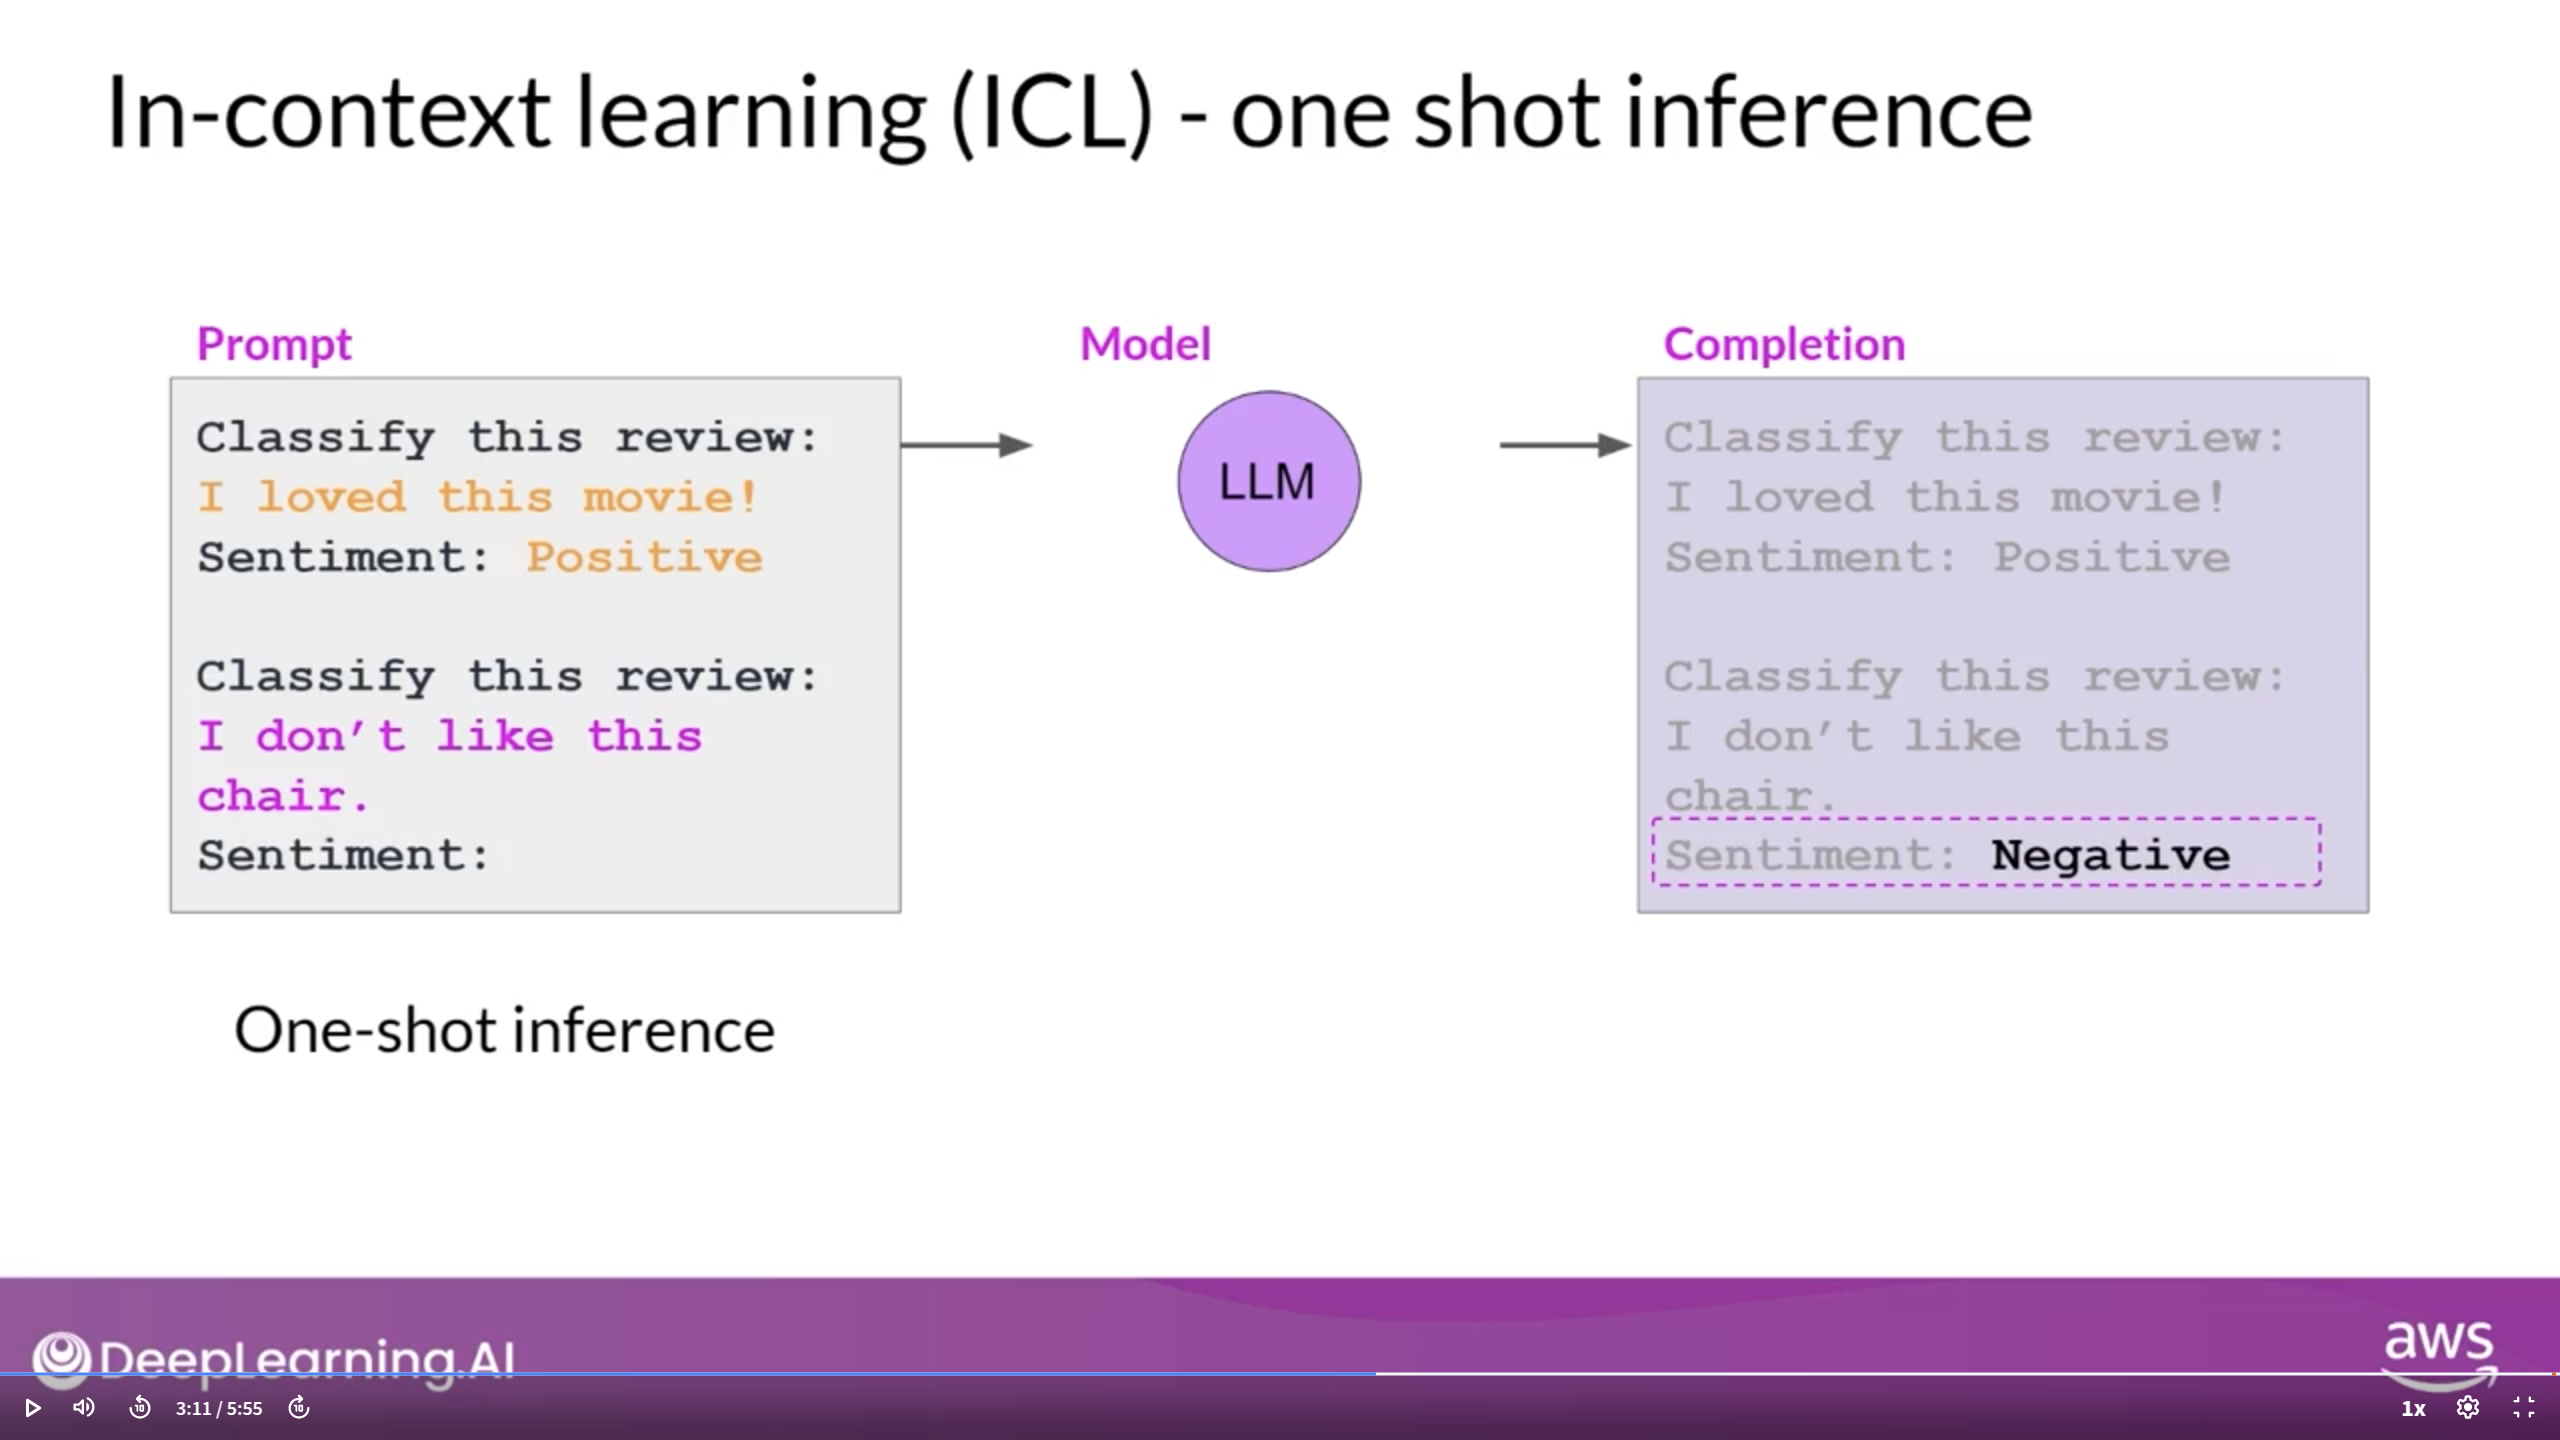
\includegraphics[trim=3cm 7cm 5cm 0cm,clip,scale=0.1]{pics/oneshot.png}
    %\caption{one-shot inference}
    %\label{fig:sub2}
  \end{subfigure}
  \begin{subfigure}[] % {.5\textwidth}
  \centering
  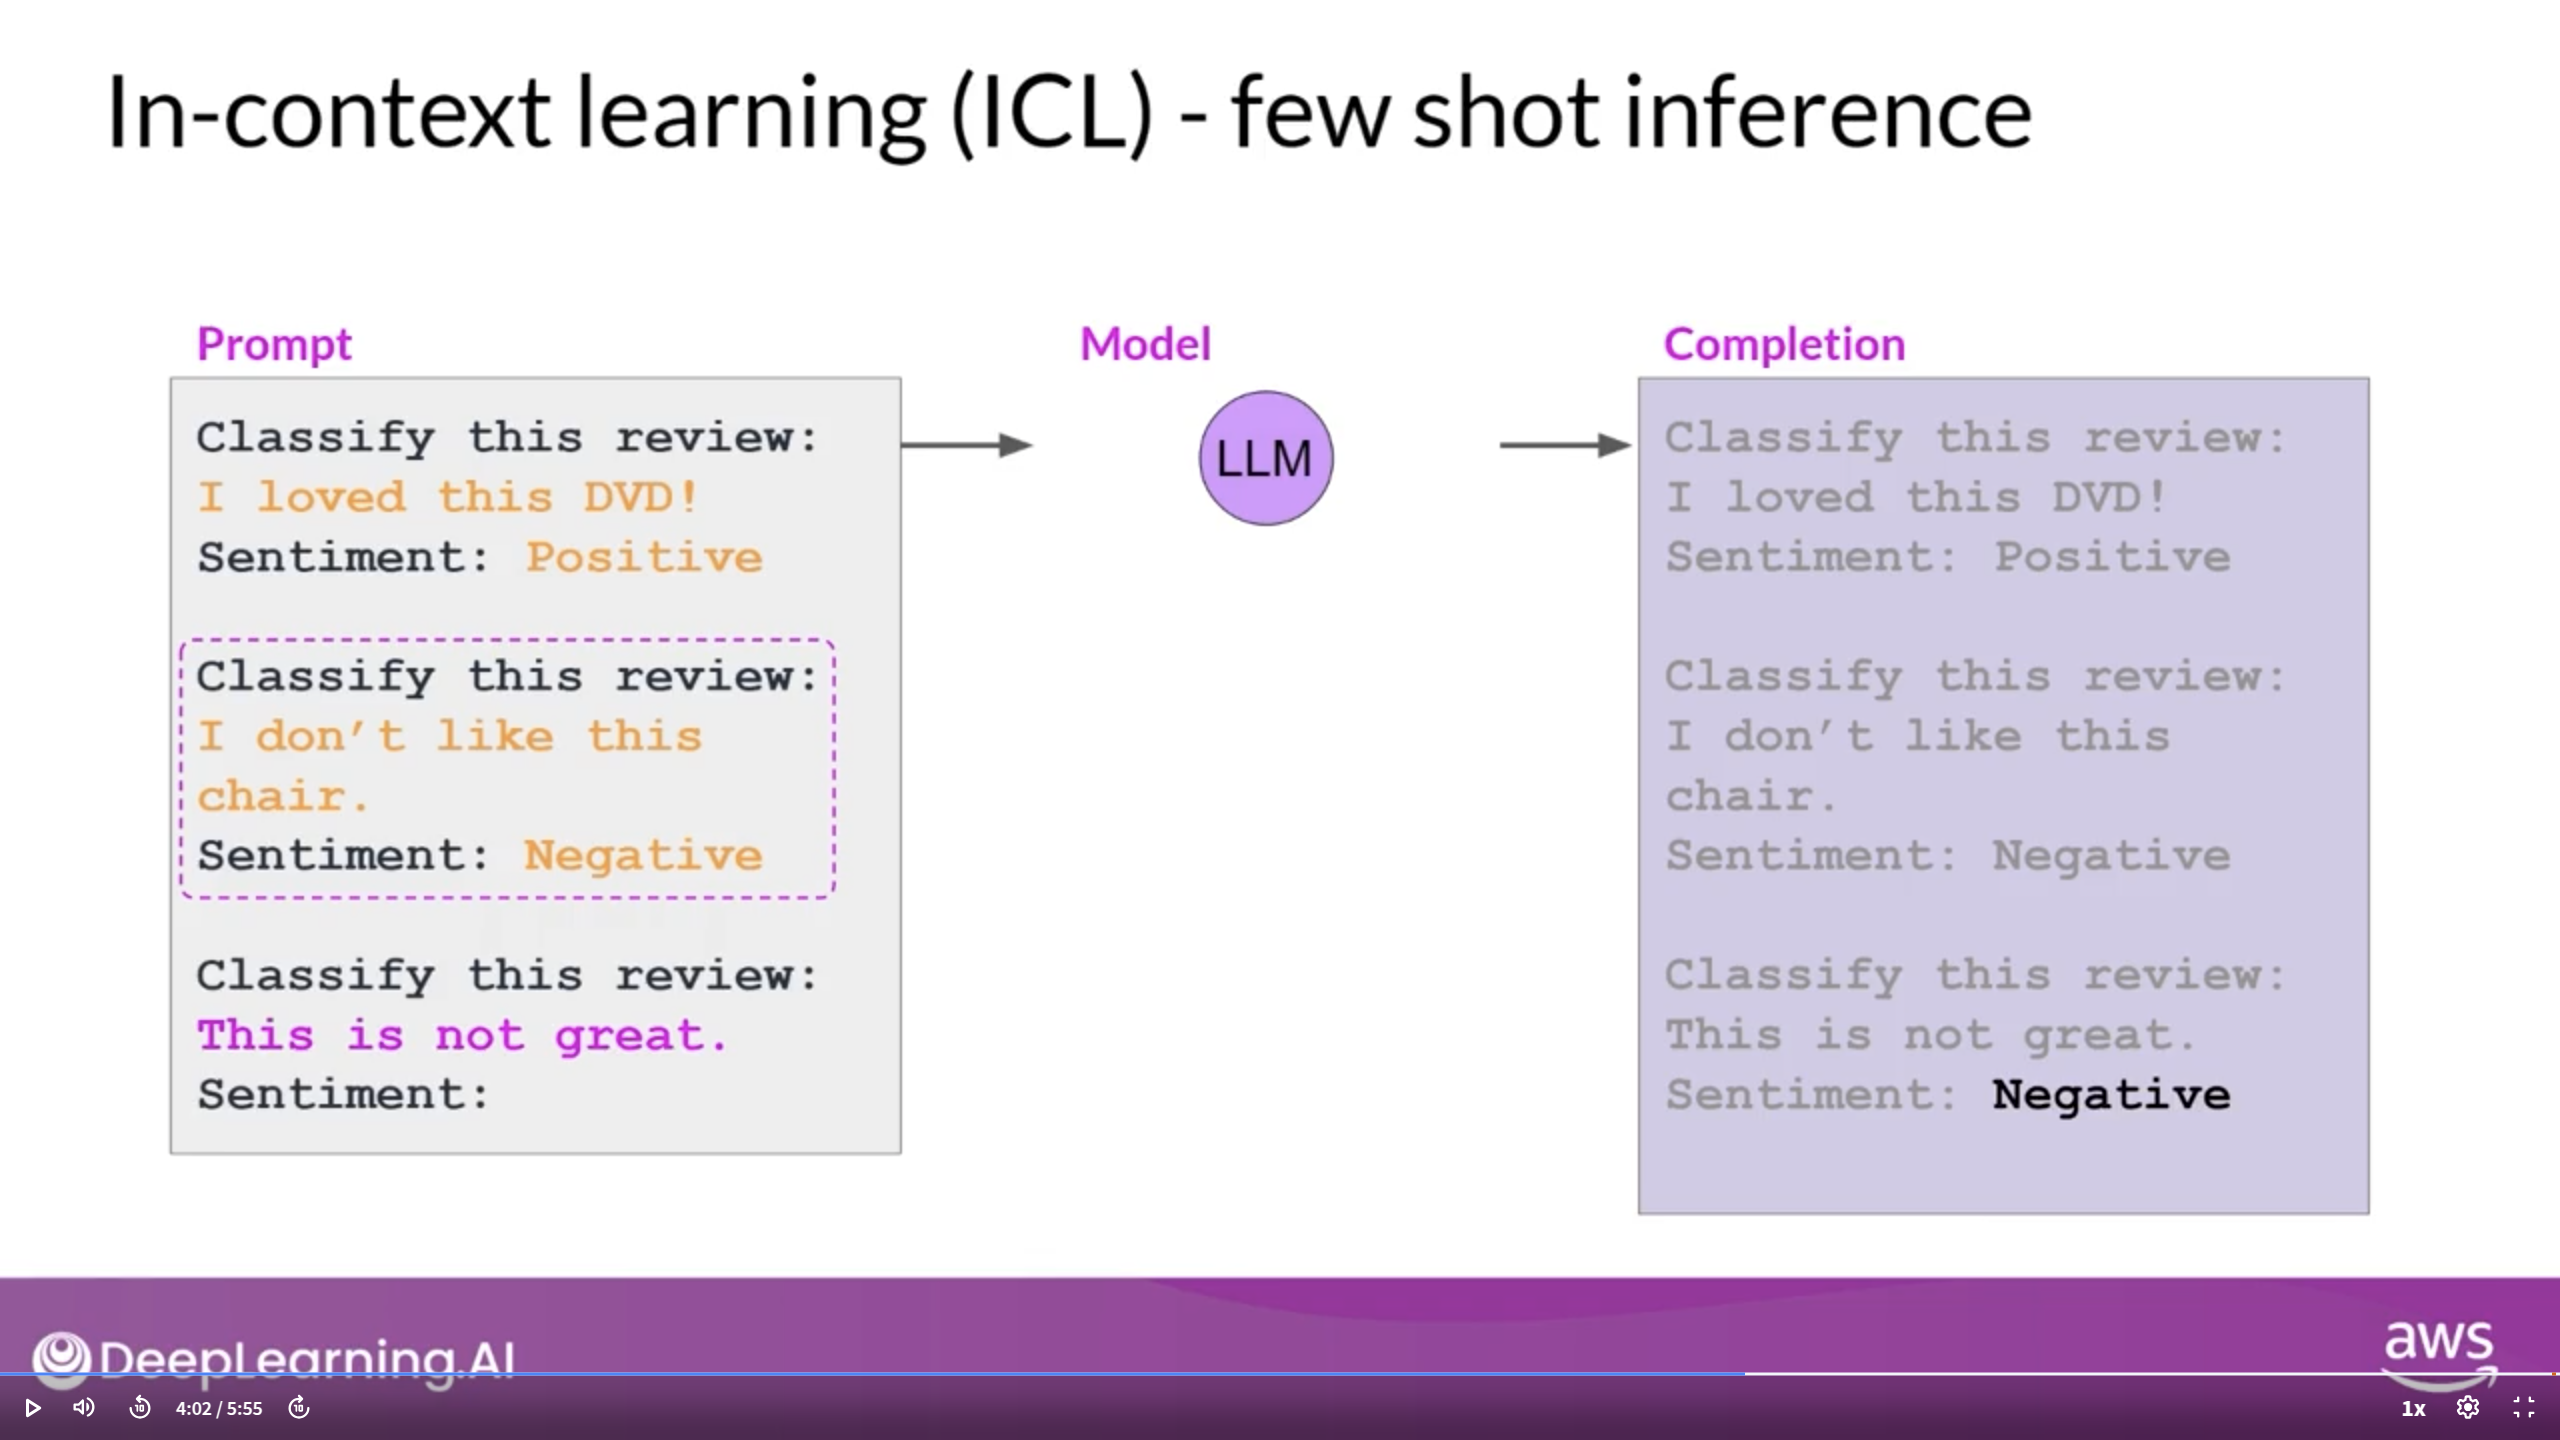
\includegraphics[trim=3cm 7cm 5cm 0cm,clip,scale=0.1]{pics/fewshot.png}
  %\caption{few-shot inference}
  %\label{fig:sub2}
  \end{subfigure}
  \caption{Prompt engineering: (a) zero-shot inference, (b) one-shot inference, (c) few-shot inference}
  %\label{fig:test}
\end{figure}

To control LLM behaviors we can set configuration parameters that are different from the training parameters. They invoked at inference time. There are at least four parameters:
\begin{enumerate}
  \item Max new tokens: Max number of tokens/output the model generate. This is like another stop condition.
  \item Sample top K\\
  The output from the LLM is a probability distribution across the entire dictionary of words that a model uses. After assigning a probability to each word, there are two modes to select the word, greedy (highest probability is selected) or random sampling (chooses the word from a random sampling using a probability distribution.)
  Greedy method is good for short generation, but it is susceptible to repeated words, or repeated sequences of words. For more natural and creative, and avoid repeating words, we can use random sampling. The output might be too creative to the point that it does not make any sense. So, we have to limit the random sampling.
  The top-K select an output from the top-k results after applying random-weighted strategy using the probabilities (choosing the from the top K highest probable tokens).

\begin{figure}[H]
  \centering
  \caption{Generative configuration}
  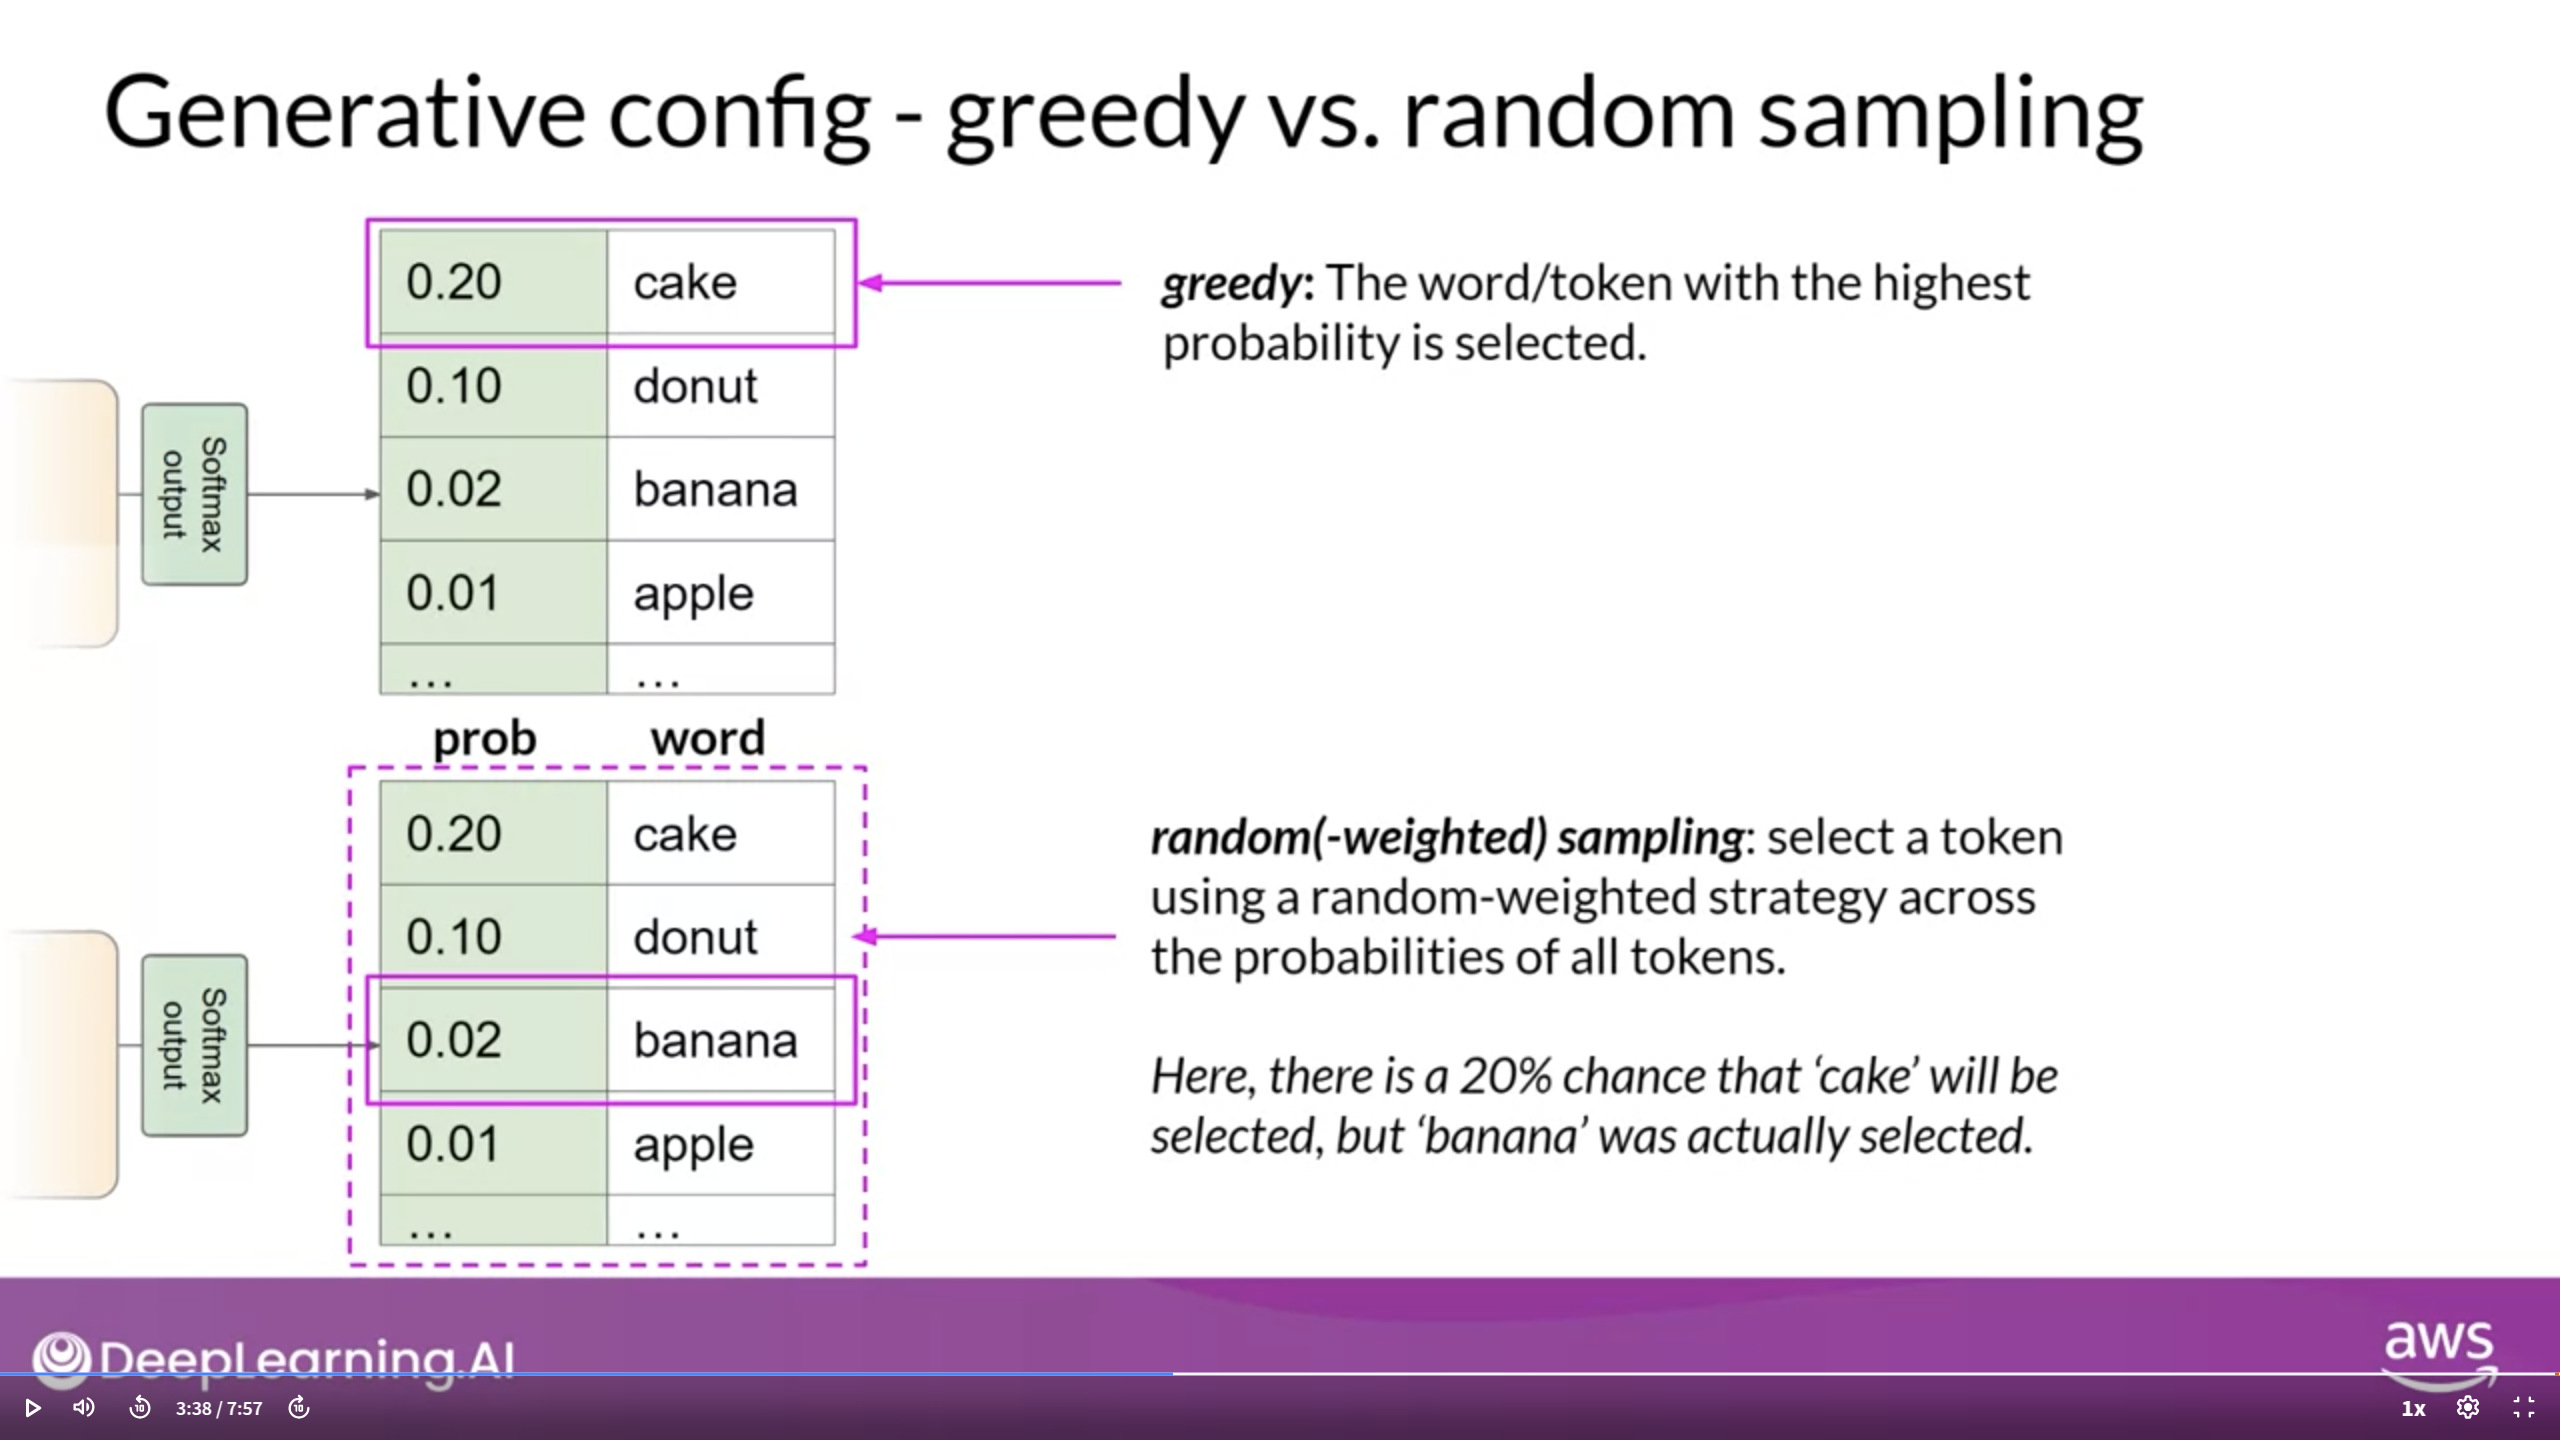
\includegraphics[trim=0cm 6cm 5cm 0cm,clip,scale=0.15]{pics/config.png}
  %{\footnotesize\textbf{Notes:} XXX.} % changed <<<<<<<<<<
  %#\label{XXX}
\end{figure}


  \item Sample top P: Select an output using the random weighted strategy with the top-ranked consecutive results by probability  and with a cumulative probability <= p.
  \item Temperature: impact the shape of probability distribution.  The higher the temperature, the higher the randomness.

  \begin{figure}[H]
    \centering
    \caption{Generative configuration}
    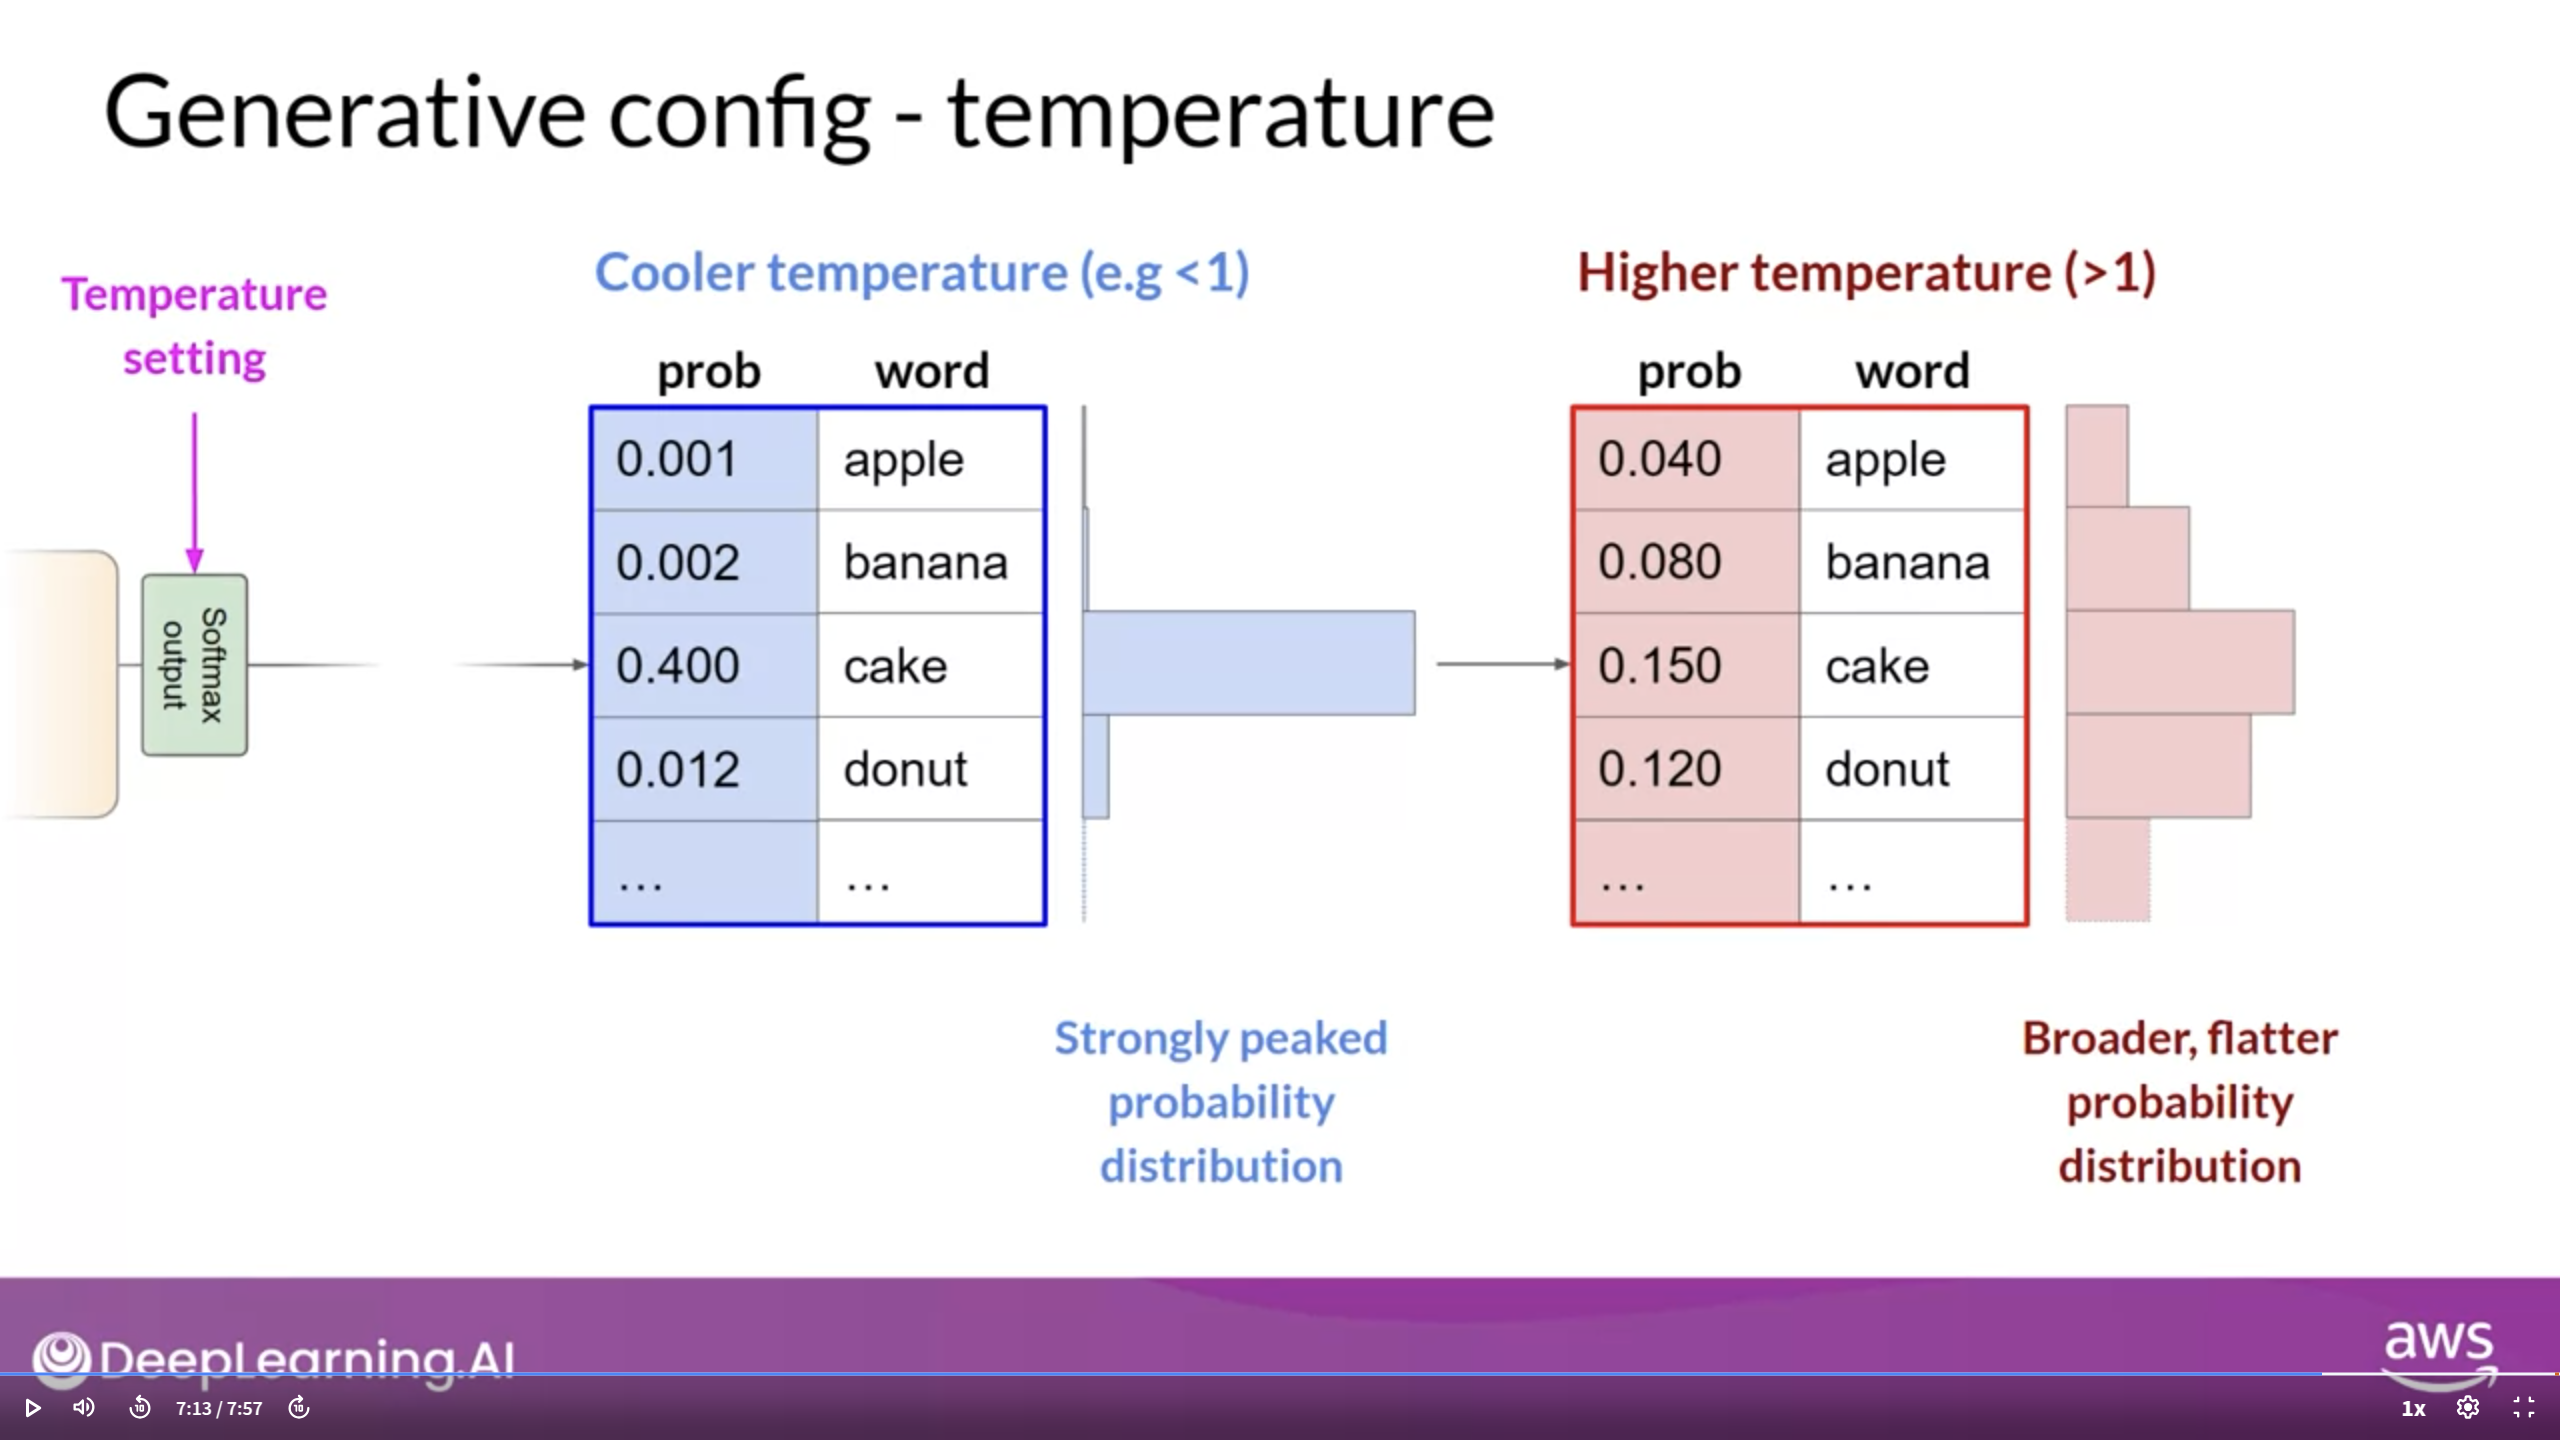
\includegraphics[trim=0cm 6cm 5cm 0cm,clip,scale=0.15]{pics/temperature.png}
    %{\footnotesize\textbf{Notes:} XXX.} % changed <<<<<<<<<<
    %#\label{XXX}
  \end{figure}
\end{enumerate}


\section{Project life cycle}
After defining the use case, we need to decide whether to use pre-trained LLMs or train your own model. To learn about the pre-trained models, we can refer to model hubs, which includes model cards that describe important details including the best use cases for each model, how it was trained, and known limitations.


\begin{figure}[H]
  \centering
  \caption{Generative AI project life cycle}
  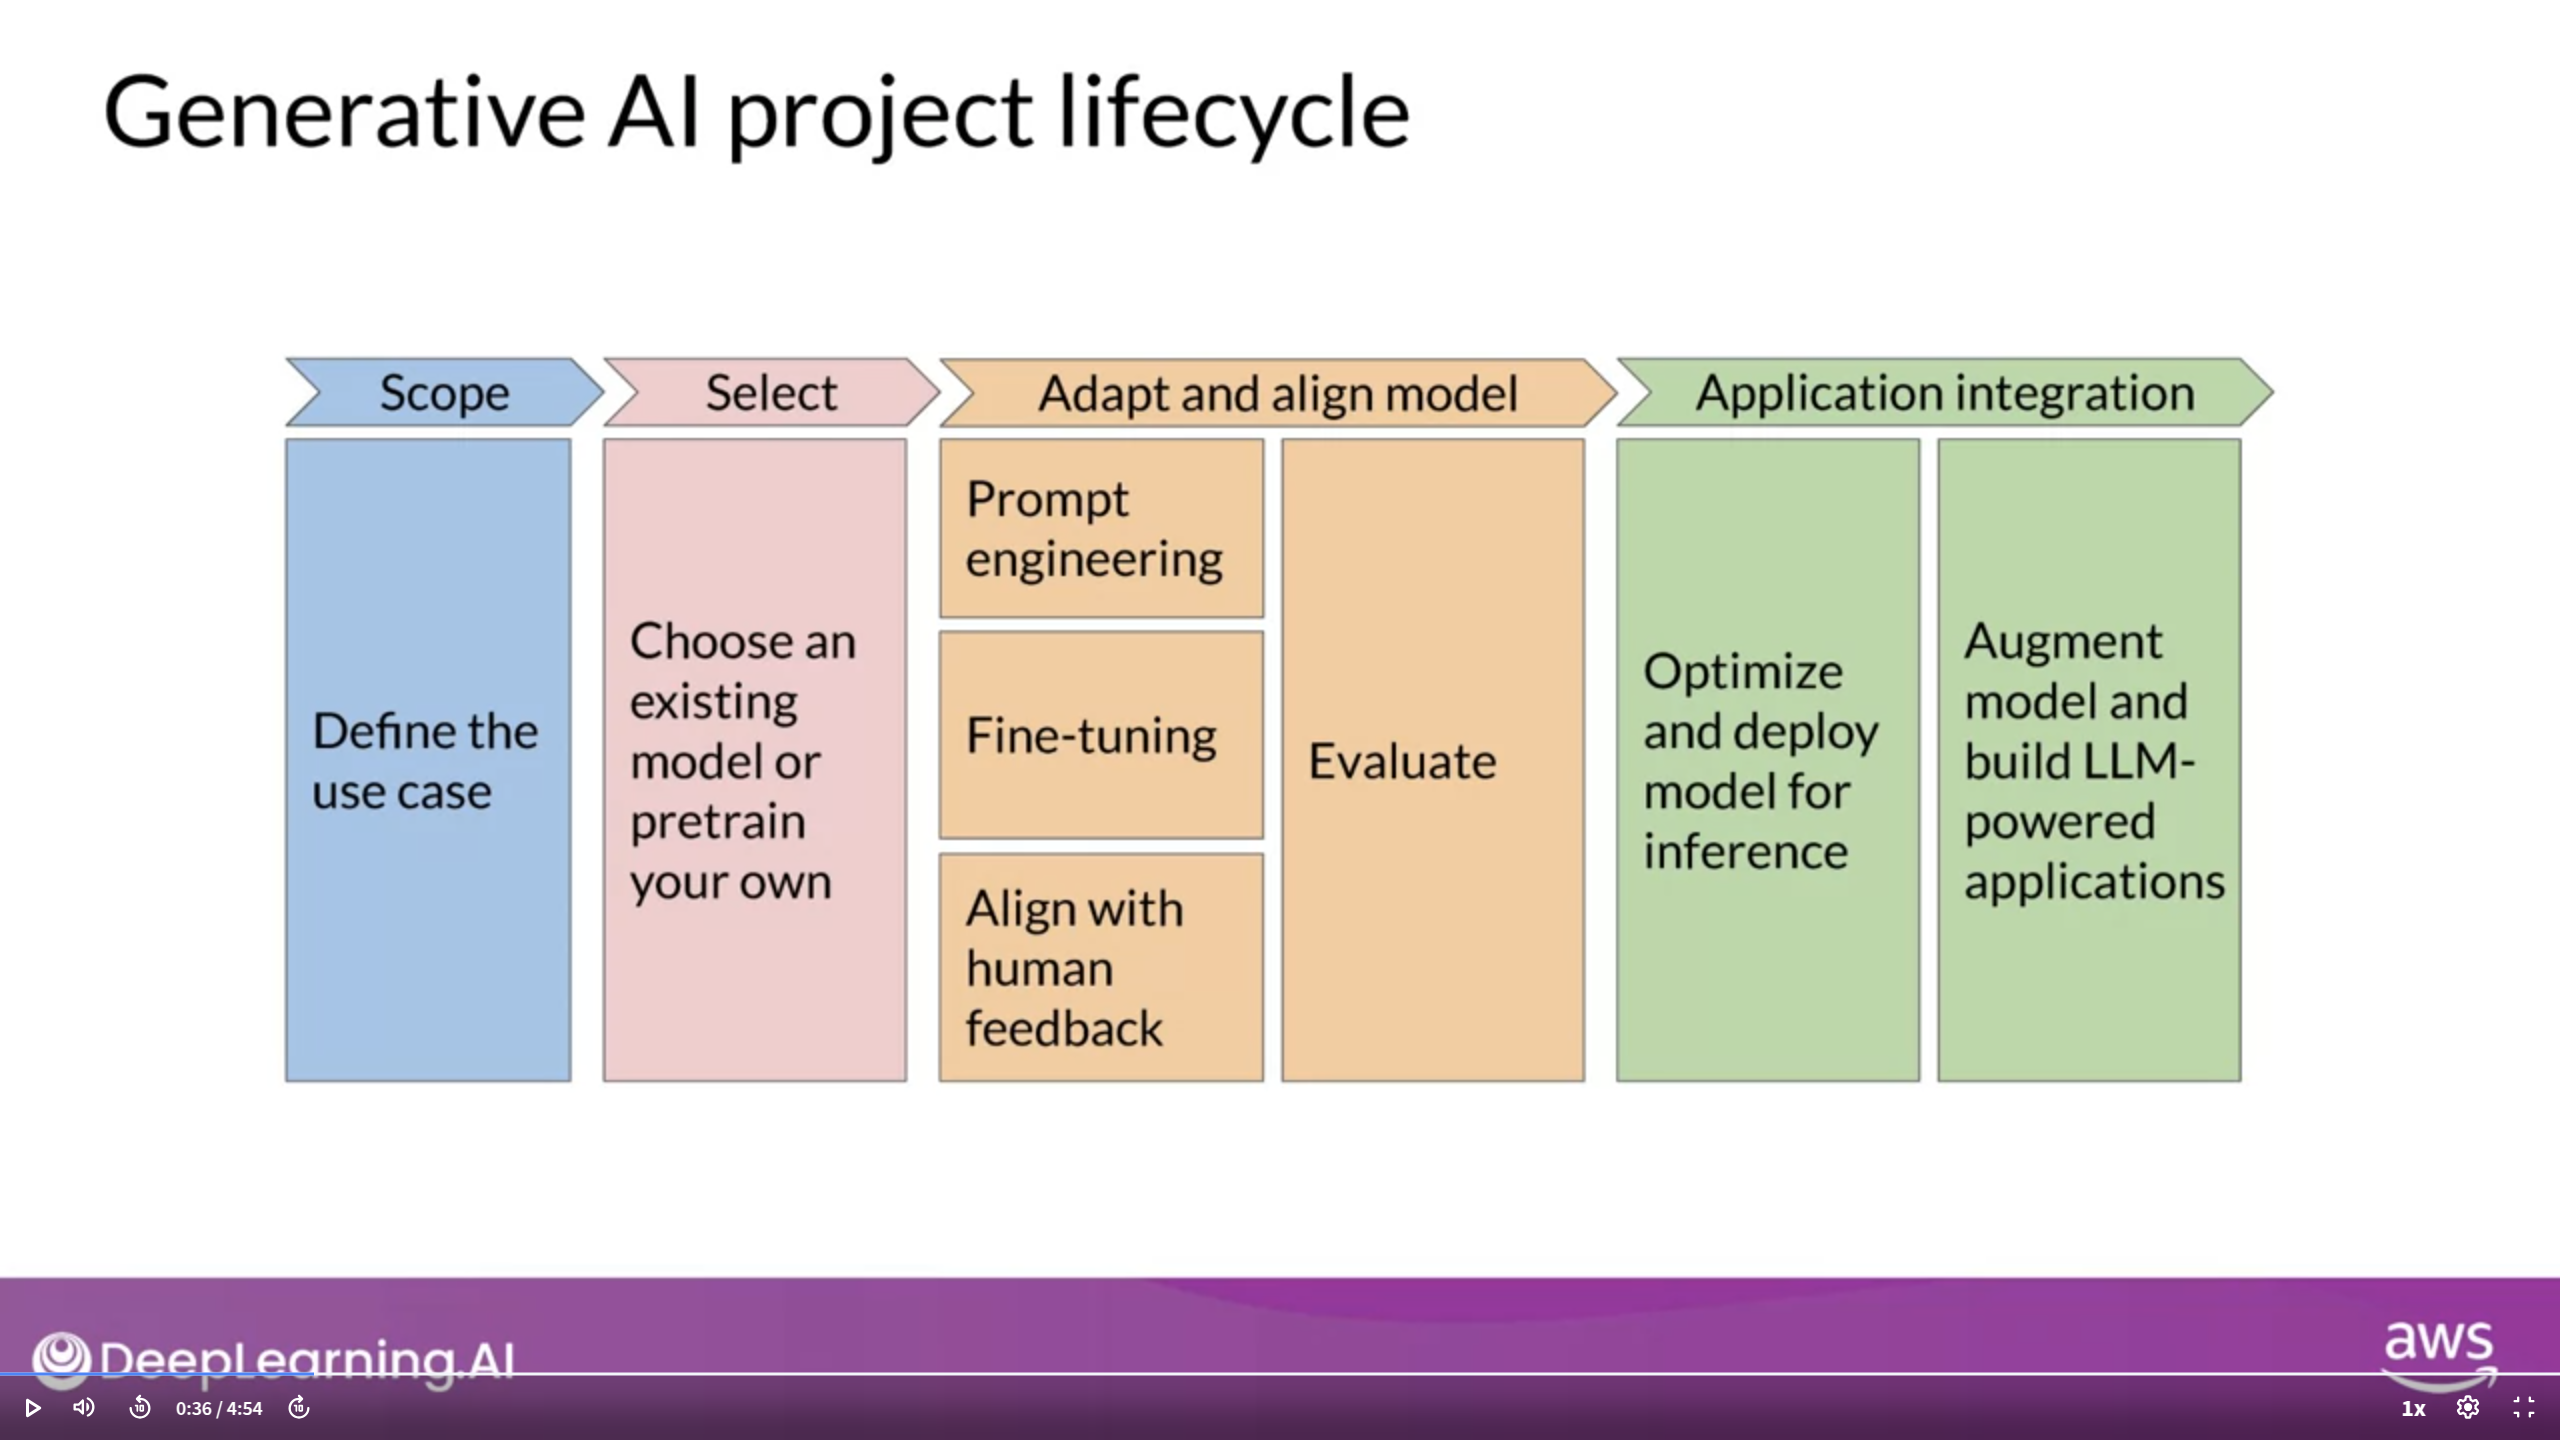
\includegraphics[trim=0cm 6cm 5cm 0cm,clip,scale=0.15]{pics/GenAILifecycle.png}
  %{\footnotesize\textbf{Notes:} XXX.} % changed <<<<<<<<<<
  %#\label{XXX}
\end{figure}



\section{Quantization}
To do the massive computation for training, we need a lot of memory, which might not be available. By quantization, we can use lower precision datatypes, to be able to fit the model on the GPU memory.

\begin{figure}
  \centering
  \begin{subfigure}[] %{.5\textwidth}
    \centering
  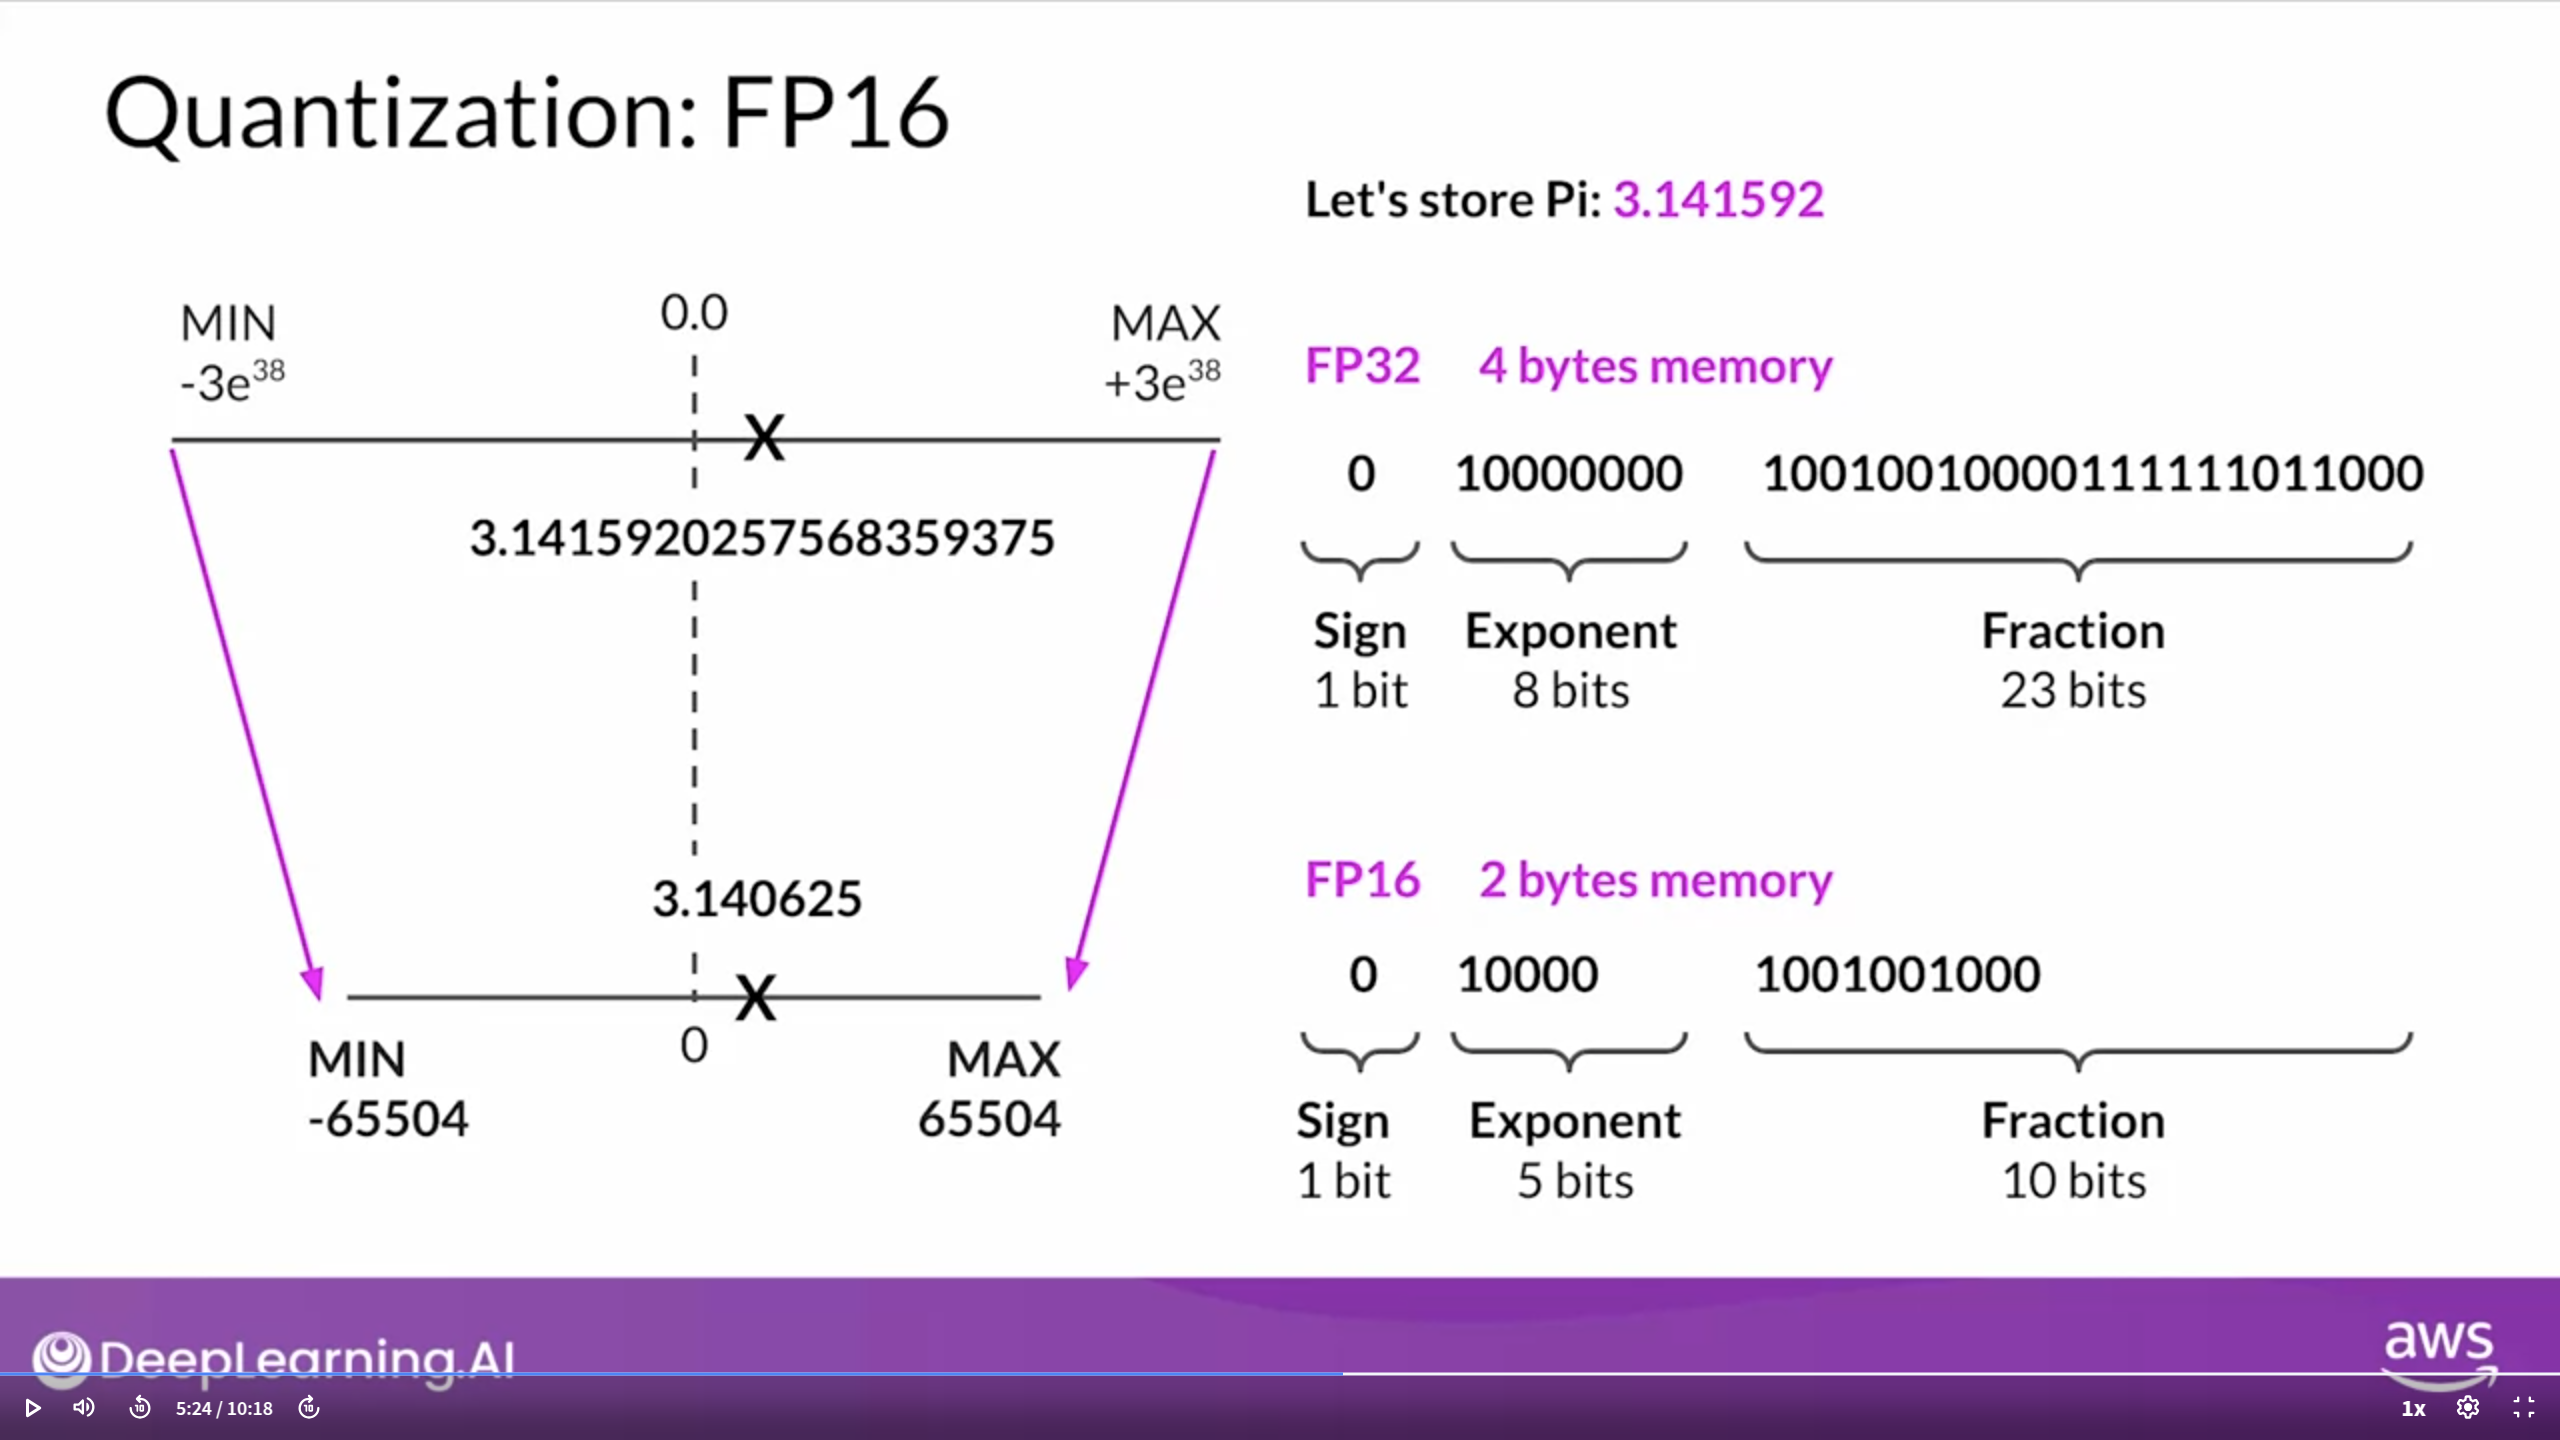
\includegraphics[trim=0cm 6cm 5cm 0cm,clip,scale=0.15]{pics/F16.png}
    %\caption{}
    %\label{fig:sub1}
  \end{subfigure}%
  \begin{subfigure}[] % {.5\textwidth}
    \centering
    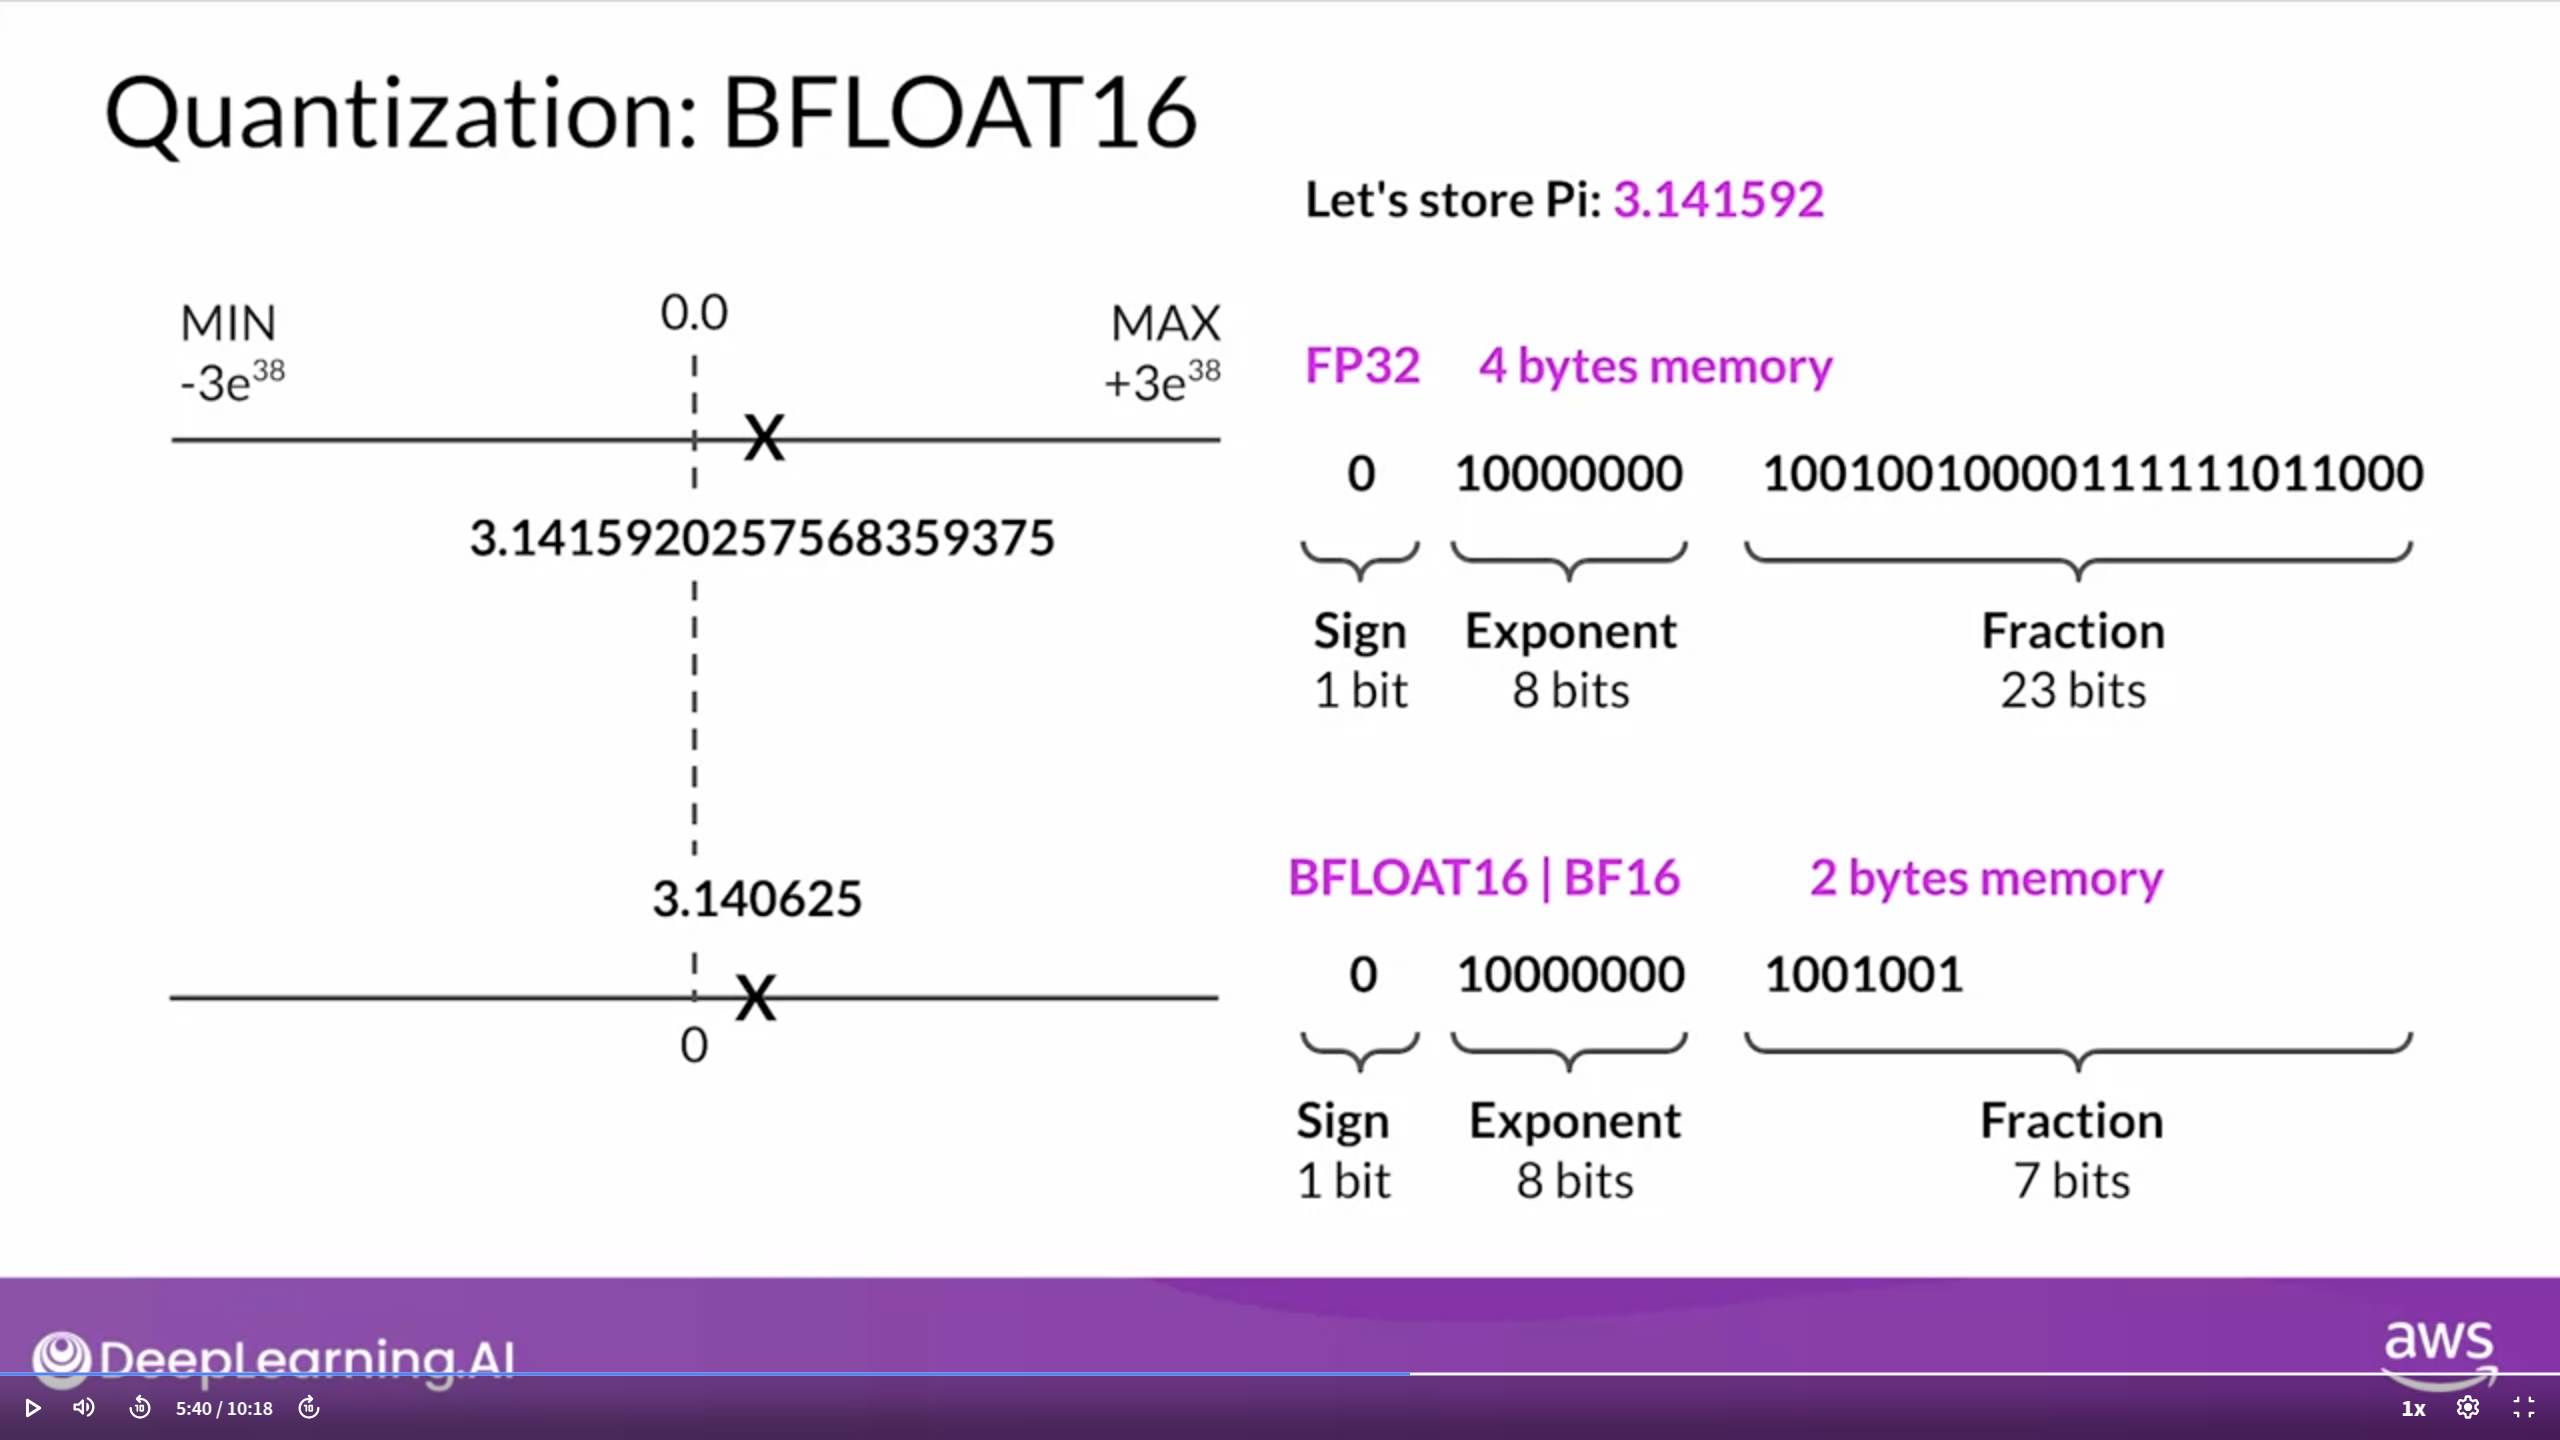
\includegraphics[trim=3cm 7cm 5cm 0cm,clip,scale=0.15]{pics/BF16.png}
    %\caption{one-shot inference}
    %\label{fig:sub2}
  \end{subfigure}
  \caption{Quantization: (a) F16, (b) BF16}
  %\label{fig:test}
\end{figure}


\section{Scale computation}
When to use/scale multi-GPU compute strategies: Model too big for single GPU, or, model fits on GPU, but you want to train data in parallel (This is called Distributed Data Parallelism- DDP).

In the DDP, pytorch copies your entire model on all GPUs, and sends batches of Data to each GPU in parallel.

\begin{figure}[H]
  \centering
  \caption{Distributed Data Parallel}
  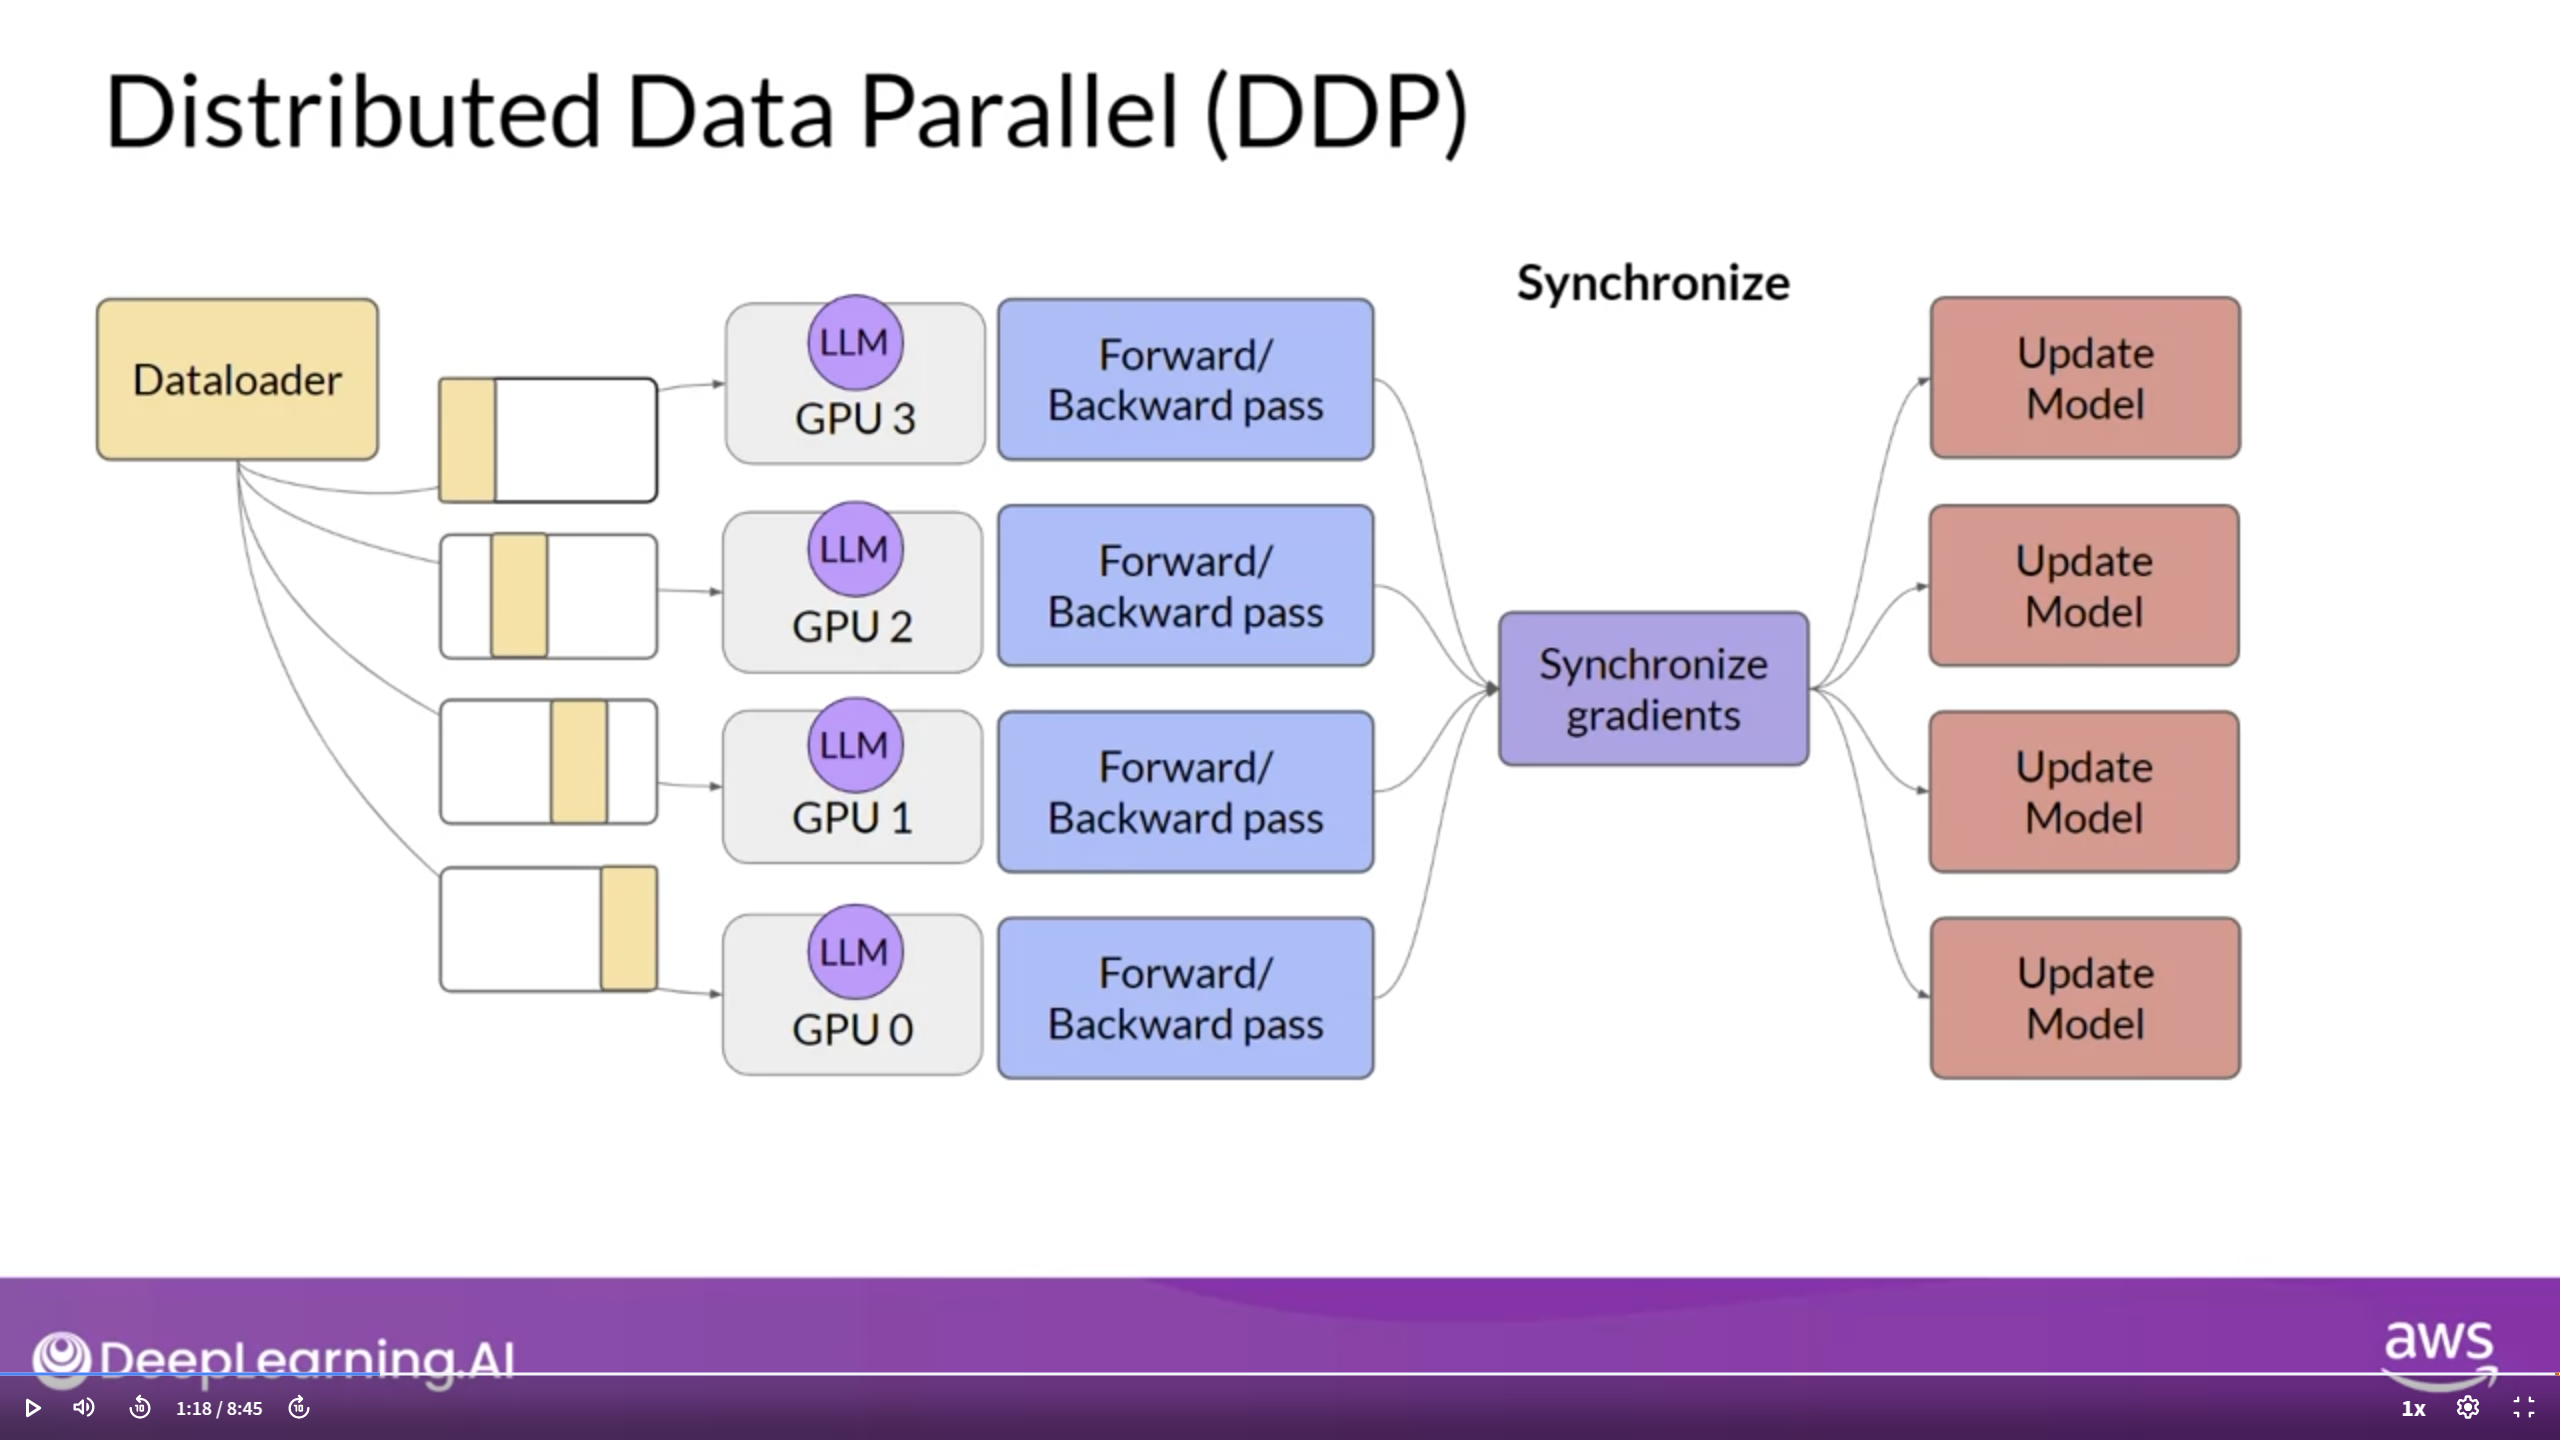
\includegraphics[trim=0cm 6cm 5cm 0cm,clip,scale=0.15]{pics/DDP.png}
  %{\footnotesize\textbf{Notes:} XXX.} % changed <<<<<<<<<<
  %#\label{XXX}
\end{figure}

The other option is Fully Sharded Data Parallel (FSDP), motivated by ZeRO (Zero Redundancy Optimizer), which allows to distribute model parameters on multiple GPUs, as opposed to DDP which stores all model parameters on each GPU. ZeRO distribute/shard the model parameters, gradients, and optimizer states across GPUs. It has three stages, depending on which model parameters are distributed. This model allows to work on models that are too big to fit on a single chip. Since not all parameters are available on a GPU, you need to Get weights from all GPUs before you run forward or backward pass. This is more like a memory vs performance trade-off decision. In short, this model, allows you to reduce overall GPU memory utilization, supports offloading to CPU if needed. To manage the trade off between performance and memory utilization, you can configure the level of sharding via sharding factor.


\begin{figure}
  \centering
  \begin{subfigure}[] %{.5\textwidth}
    \centering
    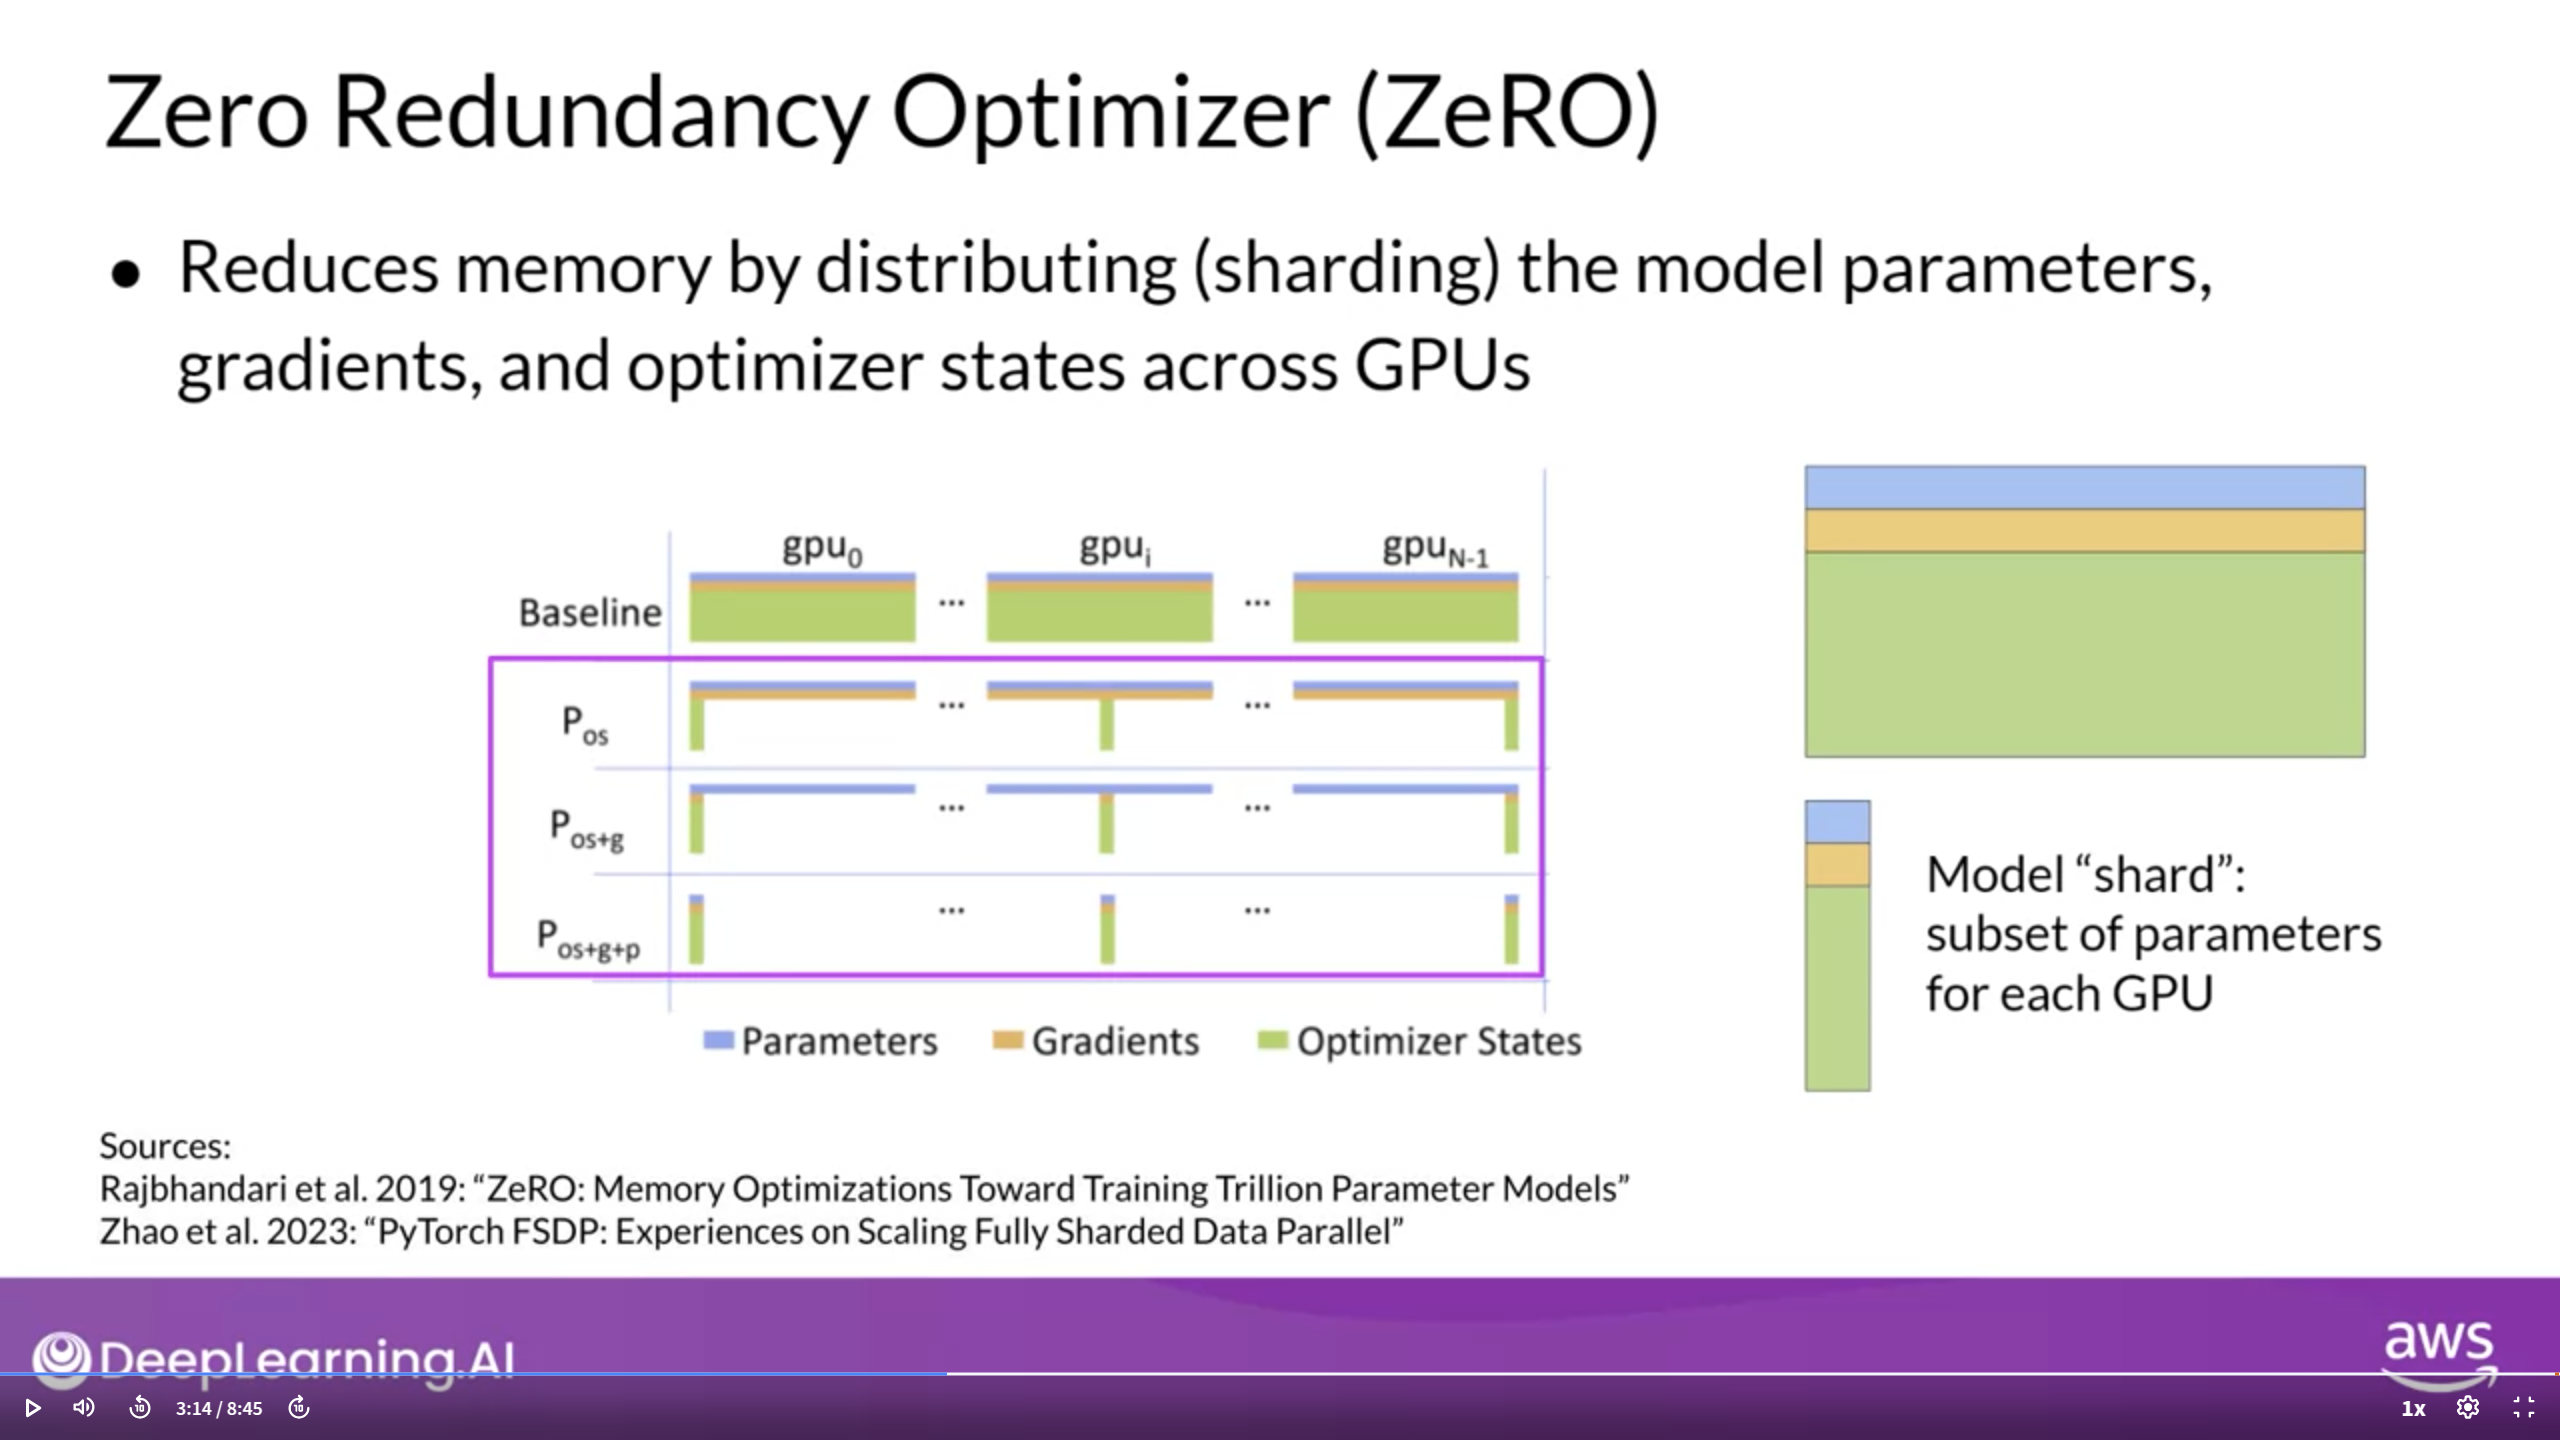
\includegraphics[trim=3cm 7cm 5cm 0cm,clip,scale=0.1]{pics/ZeRO.png}
    %\caption{}
    %\label{fig:sub1}
  \end{subfigure}%
  \begin{subfigure}[] % {.5\textwidth}
    \centering
    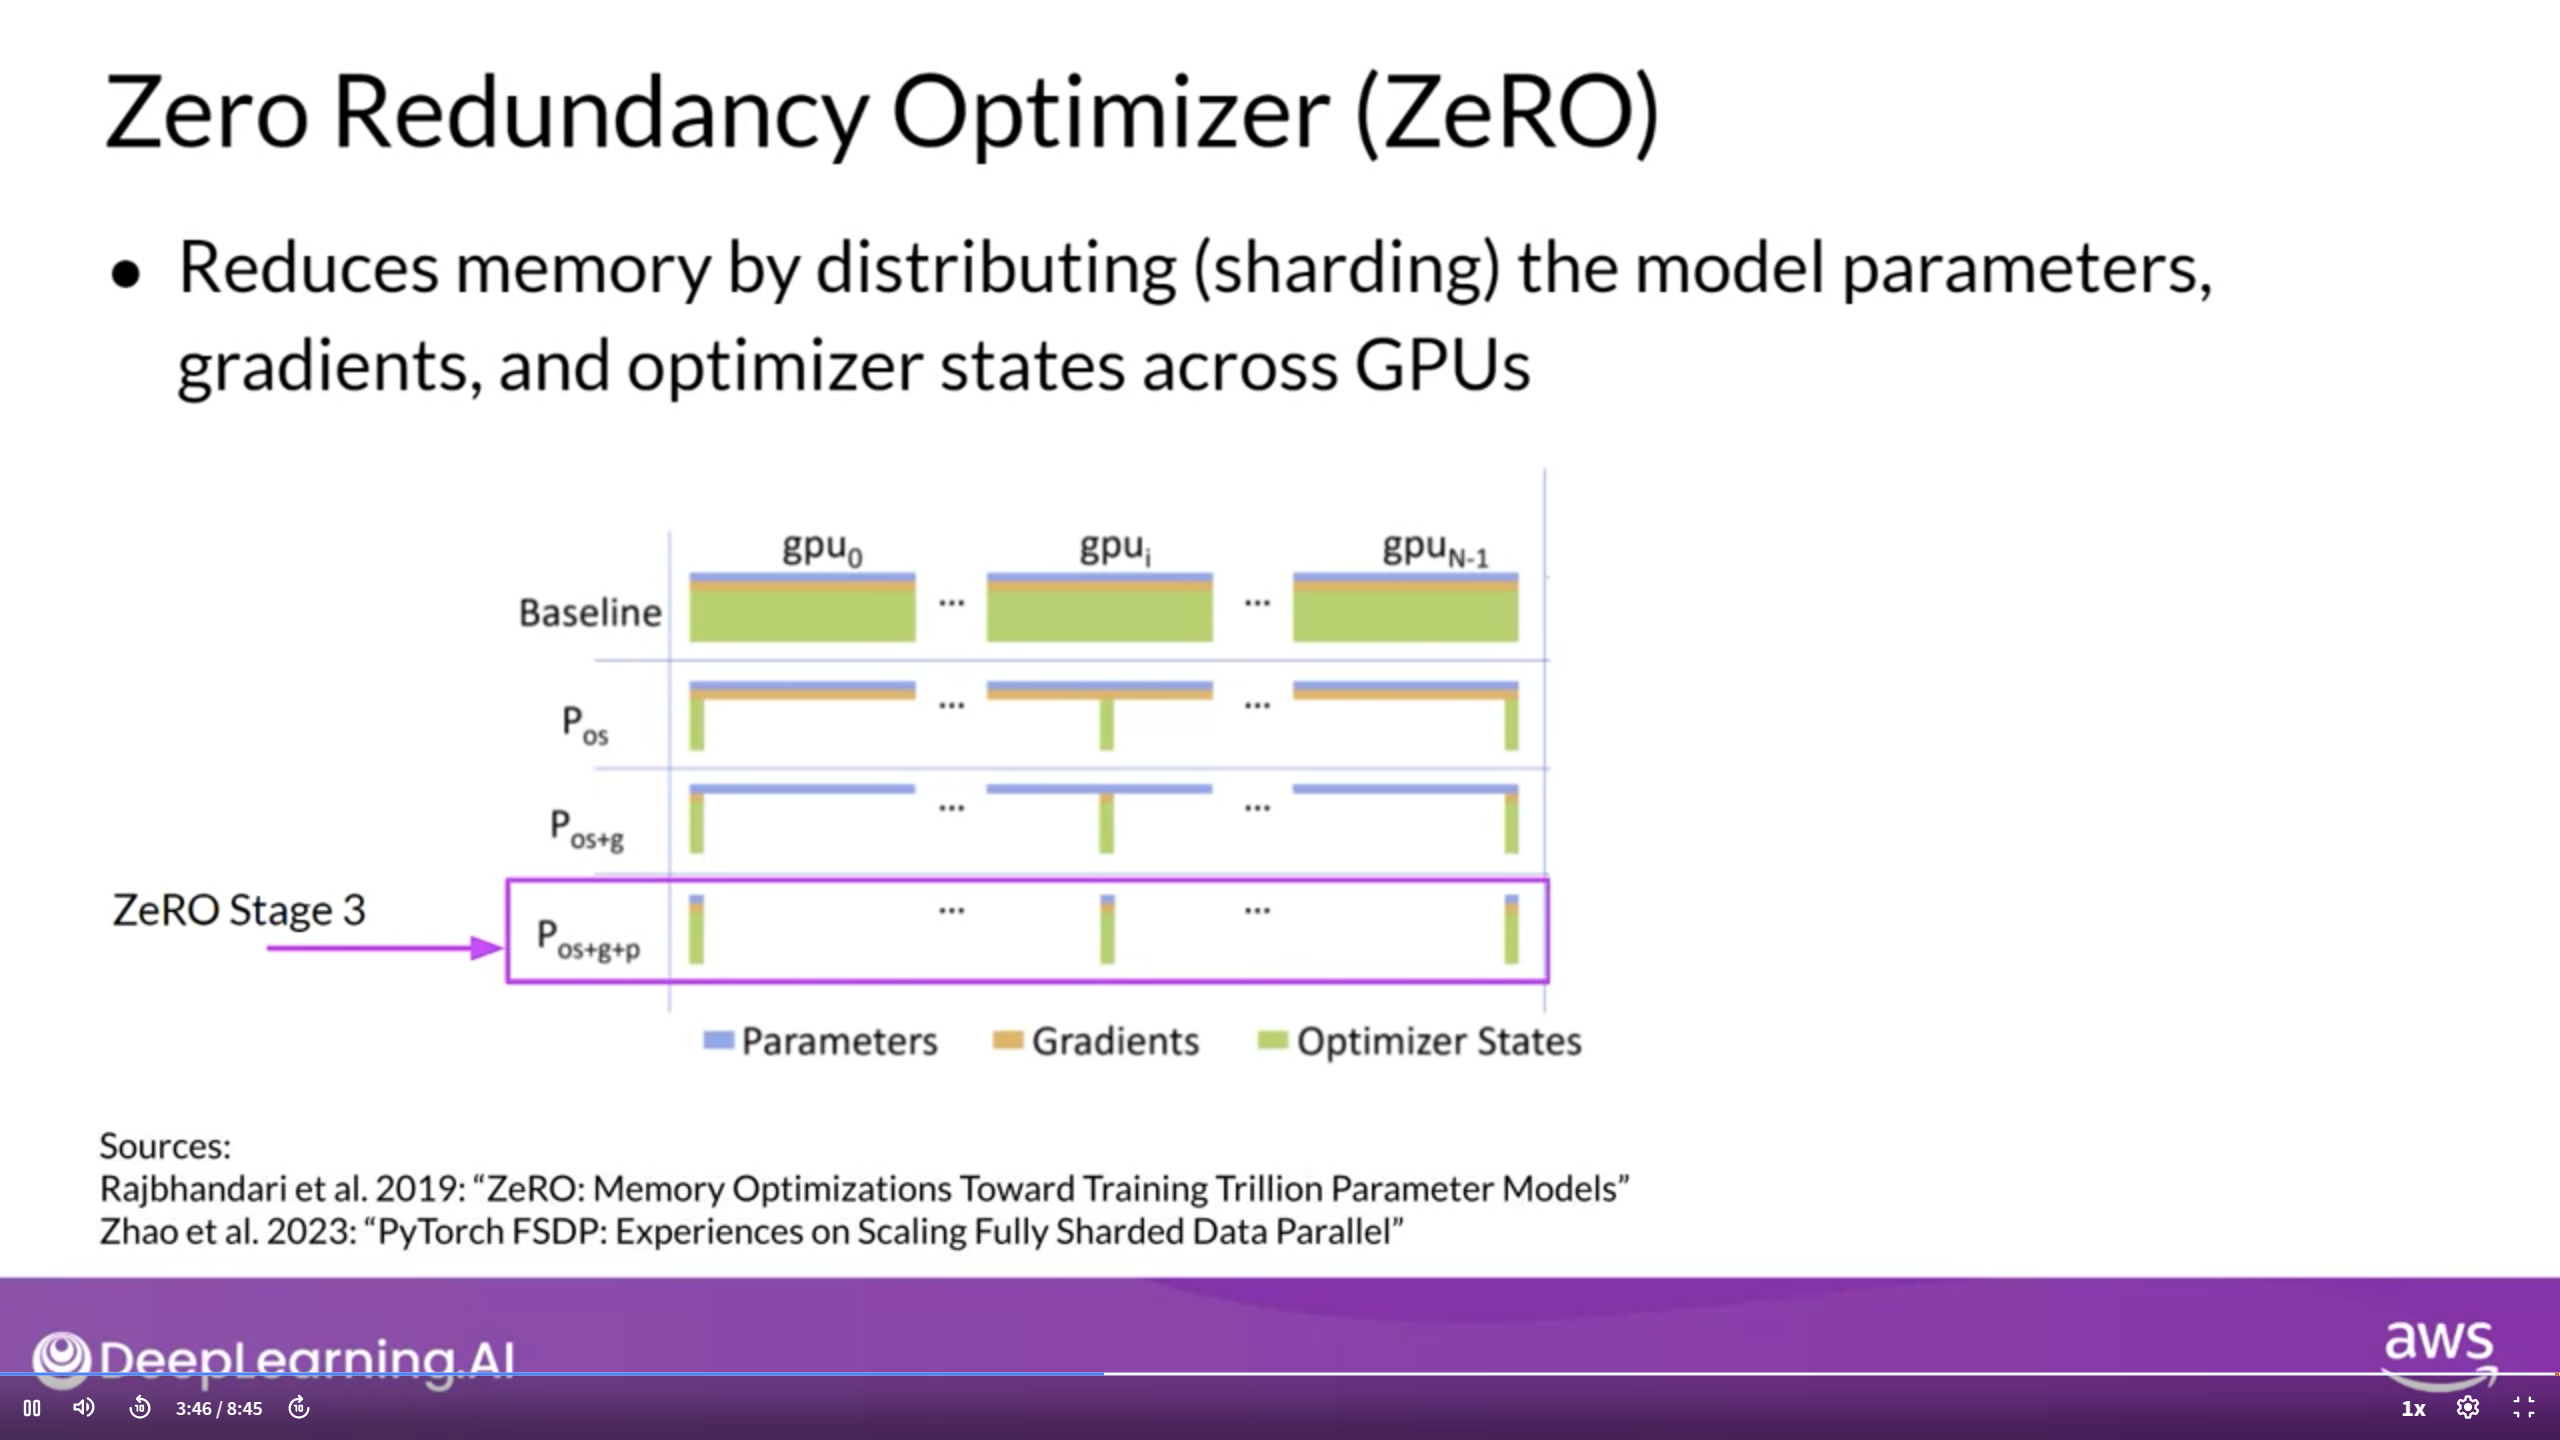
\includegraphics[trim=3cm 7cm 5cm 0cm,clip,scale=0.1]{pics/ZeRO2.png}
    %\caption{one-shot inference}
    %\label{fig:sub2}
  \end{subfigure}
  \begin{subfigure}[] % {.5\textwidth}
  \centering
  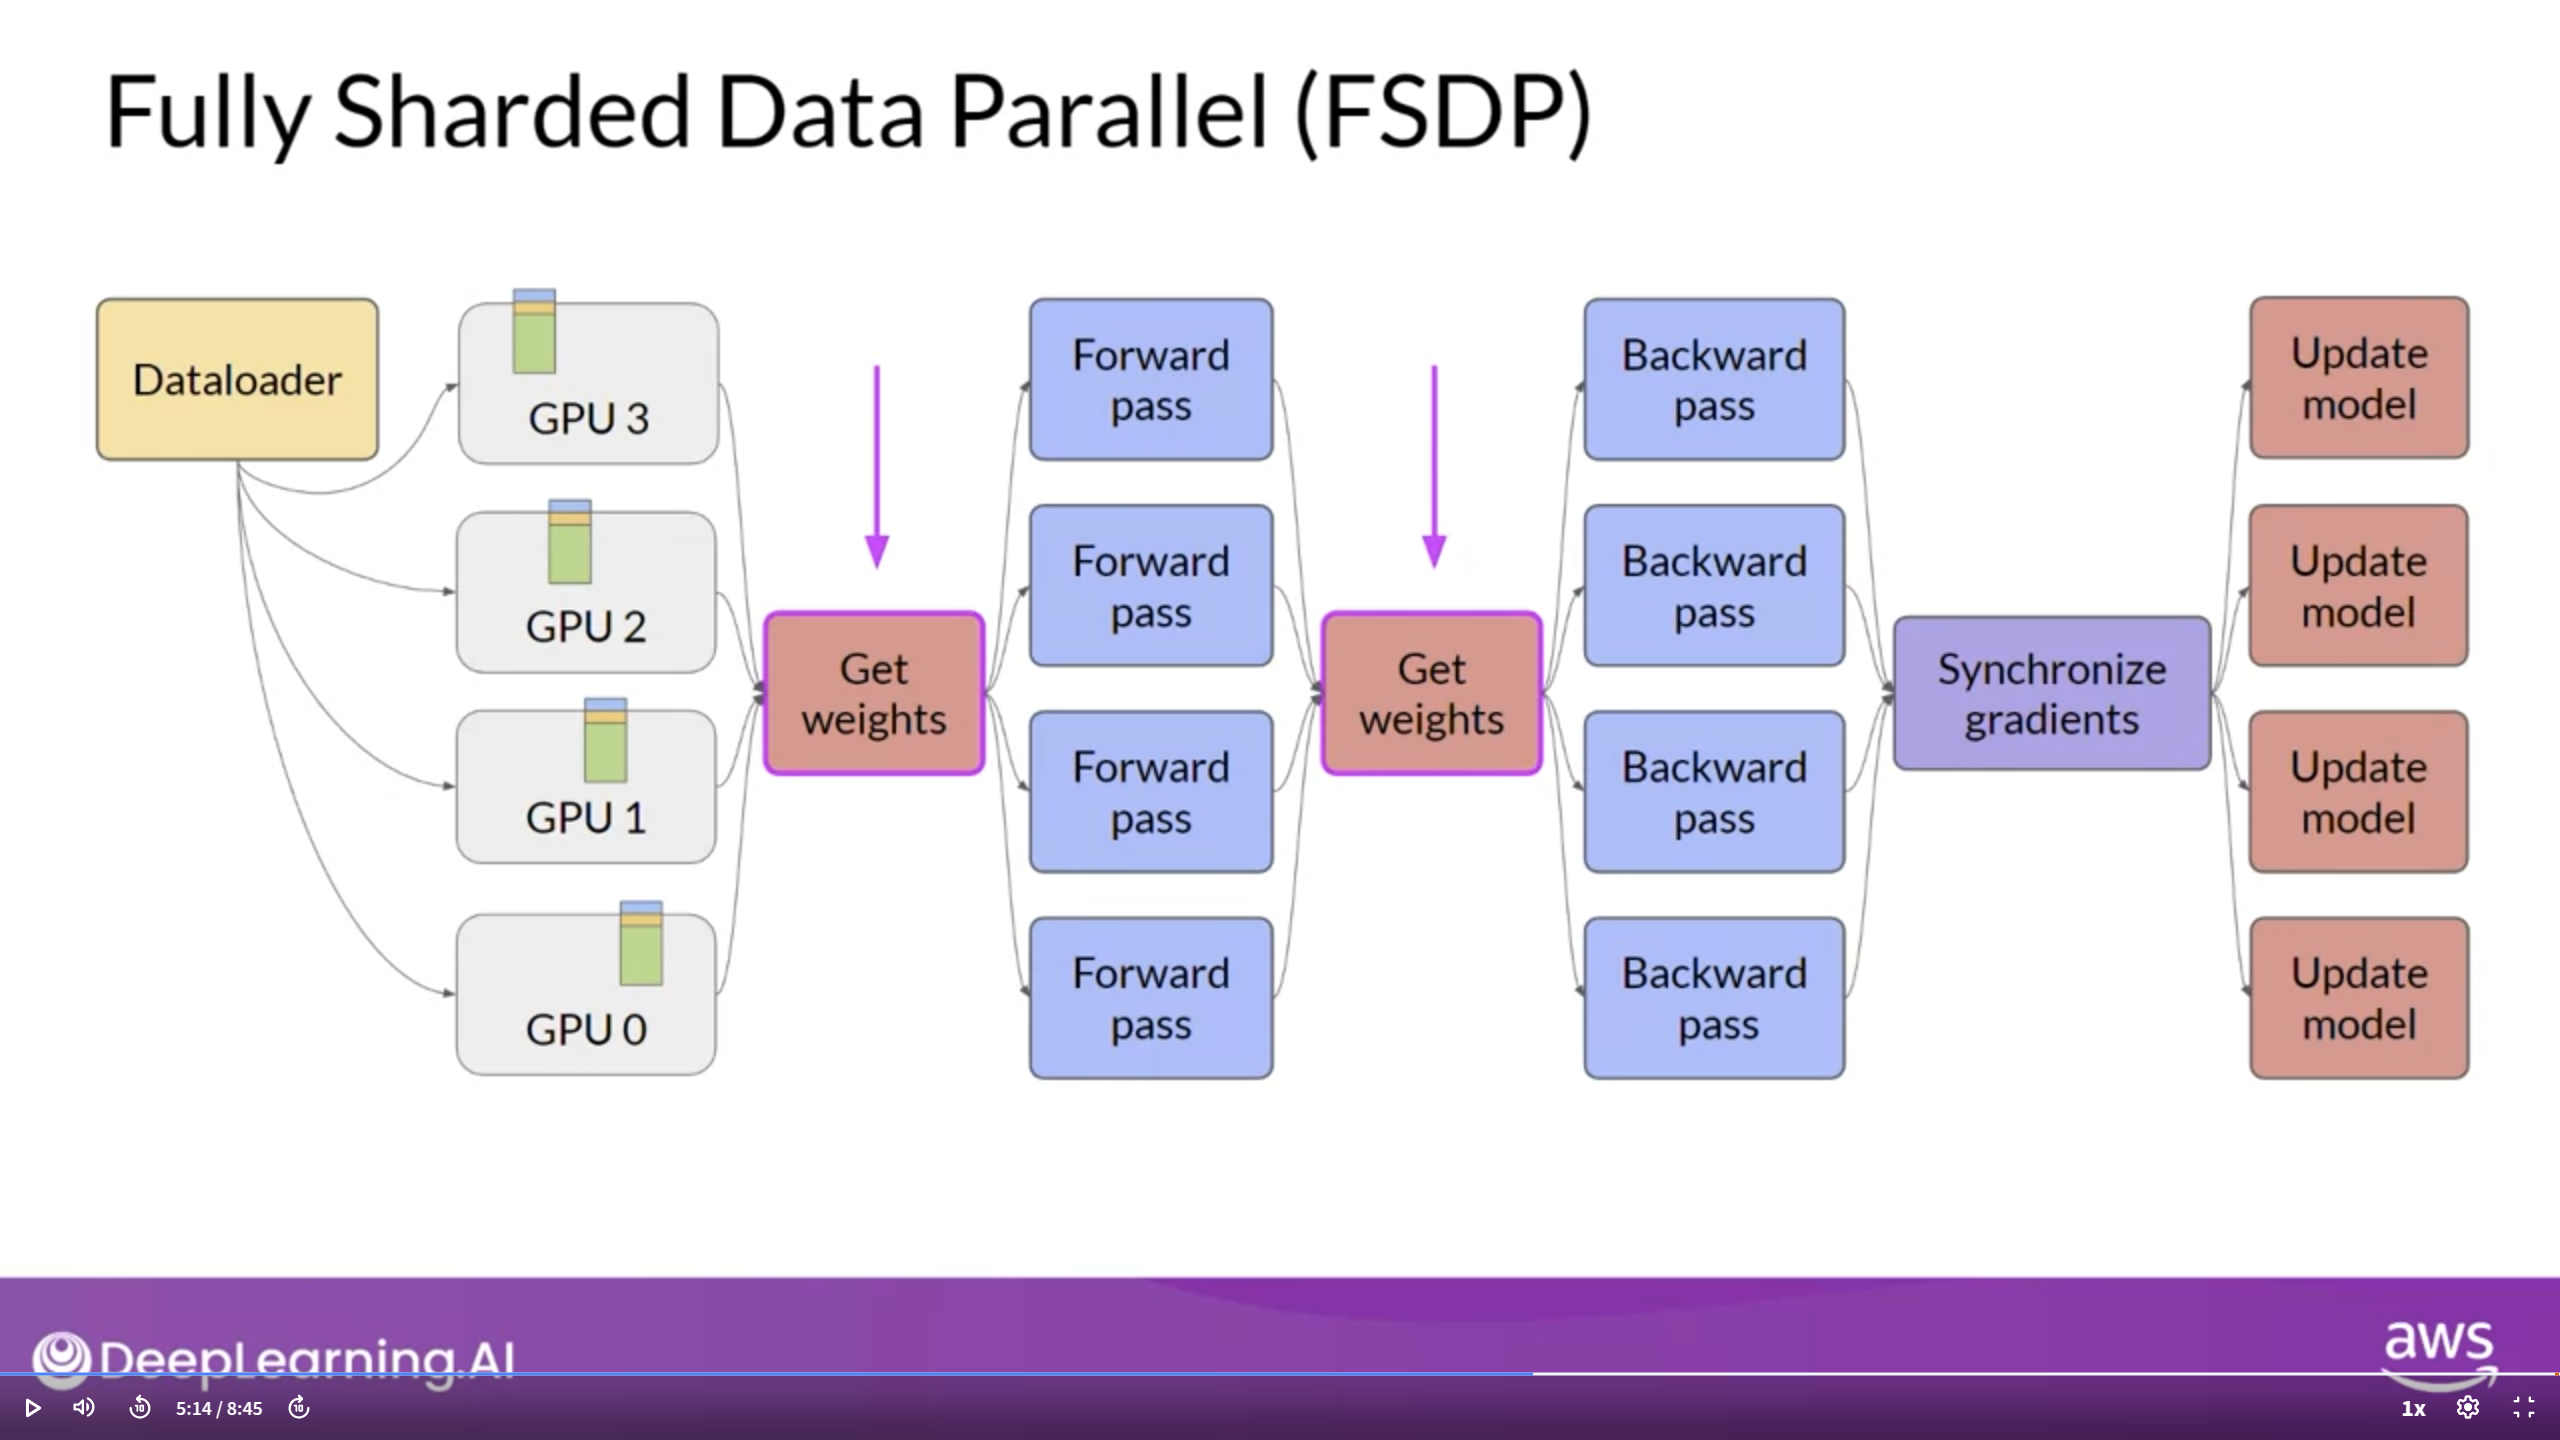
\includegraphics[trim=3cm 7cm 5cm 0cm,clip,scale=0.1]{pics/FSDP.png}
  %\caption{one-shot inference}
  %\label{fig:sub2}
  \end{subfigure}

  \caption{Multi GPU: (a) Distributing three types of model parameters, (b) Stages of ZeRO, (c) Fully Shared Data Parallel}
  %\label{fig:test}
\end{figure}


There are three factors that affects the model performance, as depicted in the following picture. The impact of each item on the model performance is linear (in the power loss chart - test loss vs parameter logarithmic chart). What is the ideal balance between these three quantities? According to the Chinchilla paper, the recommended datasize should be 20x of the model parameter size, otherwise, the model has not seen enough data. Based on the results of this paper, many models has not seen enough training data, which means that a smaller model (smaller parameters) with the right amount of data can perform the same as the large models. For this reason, some new models with smaller number of parameters developed.

\begin{figure}[H]
  \centering
  \caption{Distributed Data Parallel}
  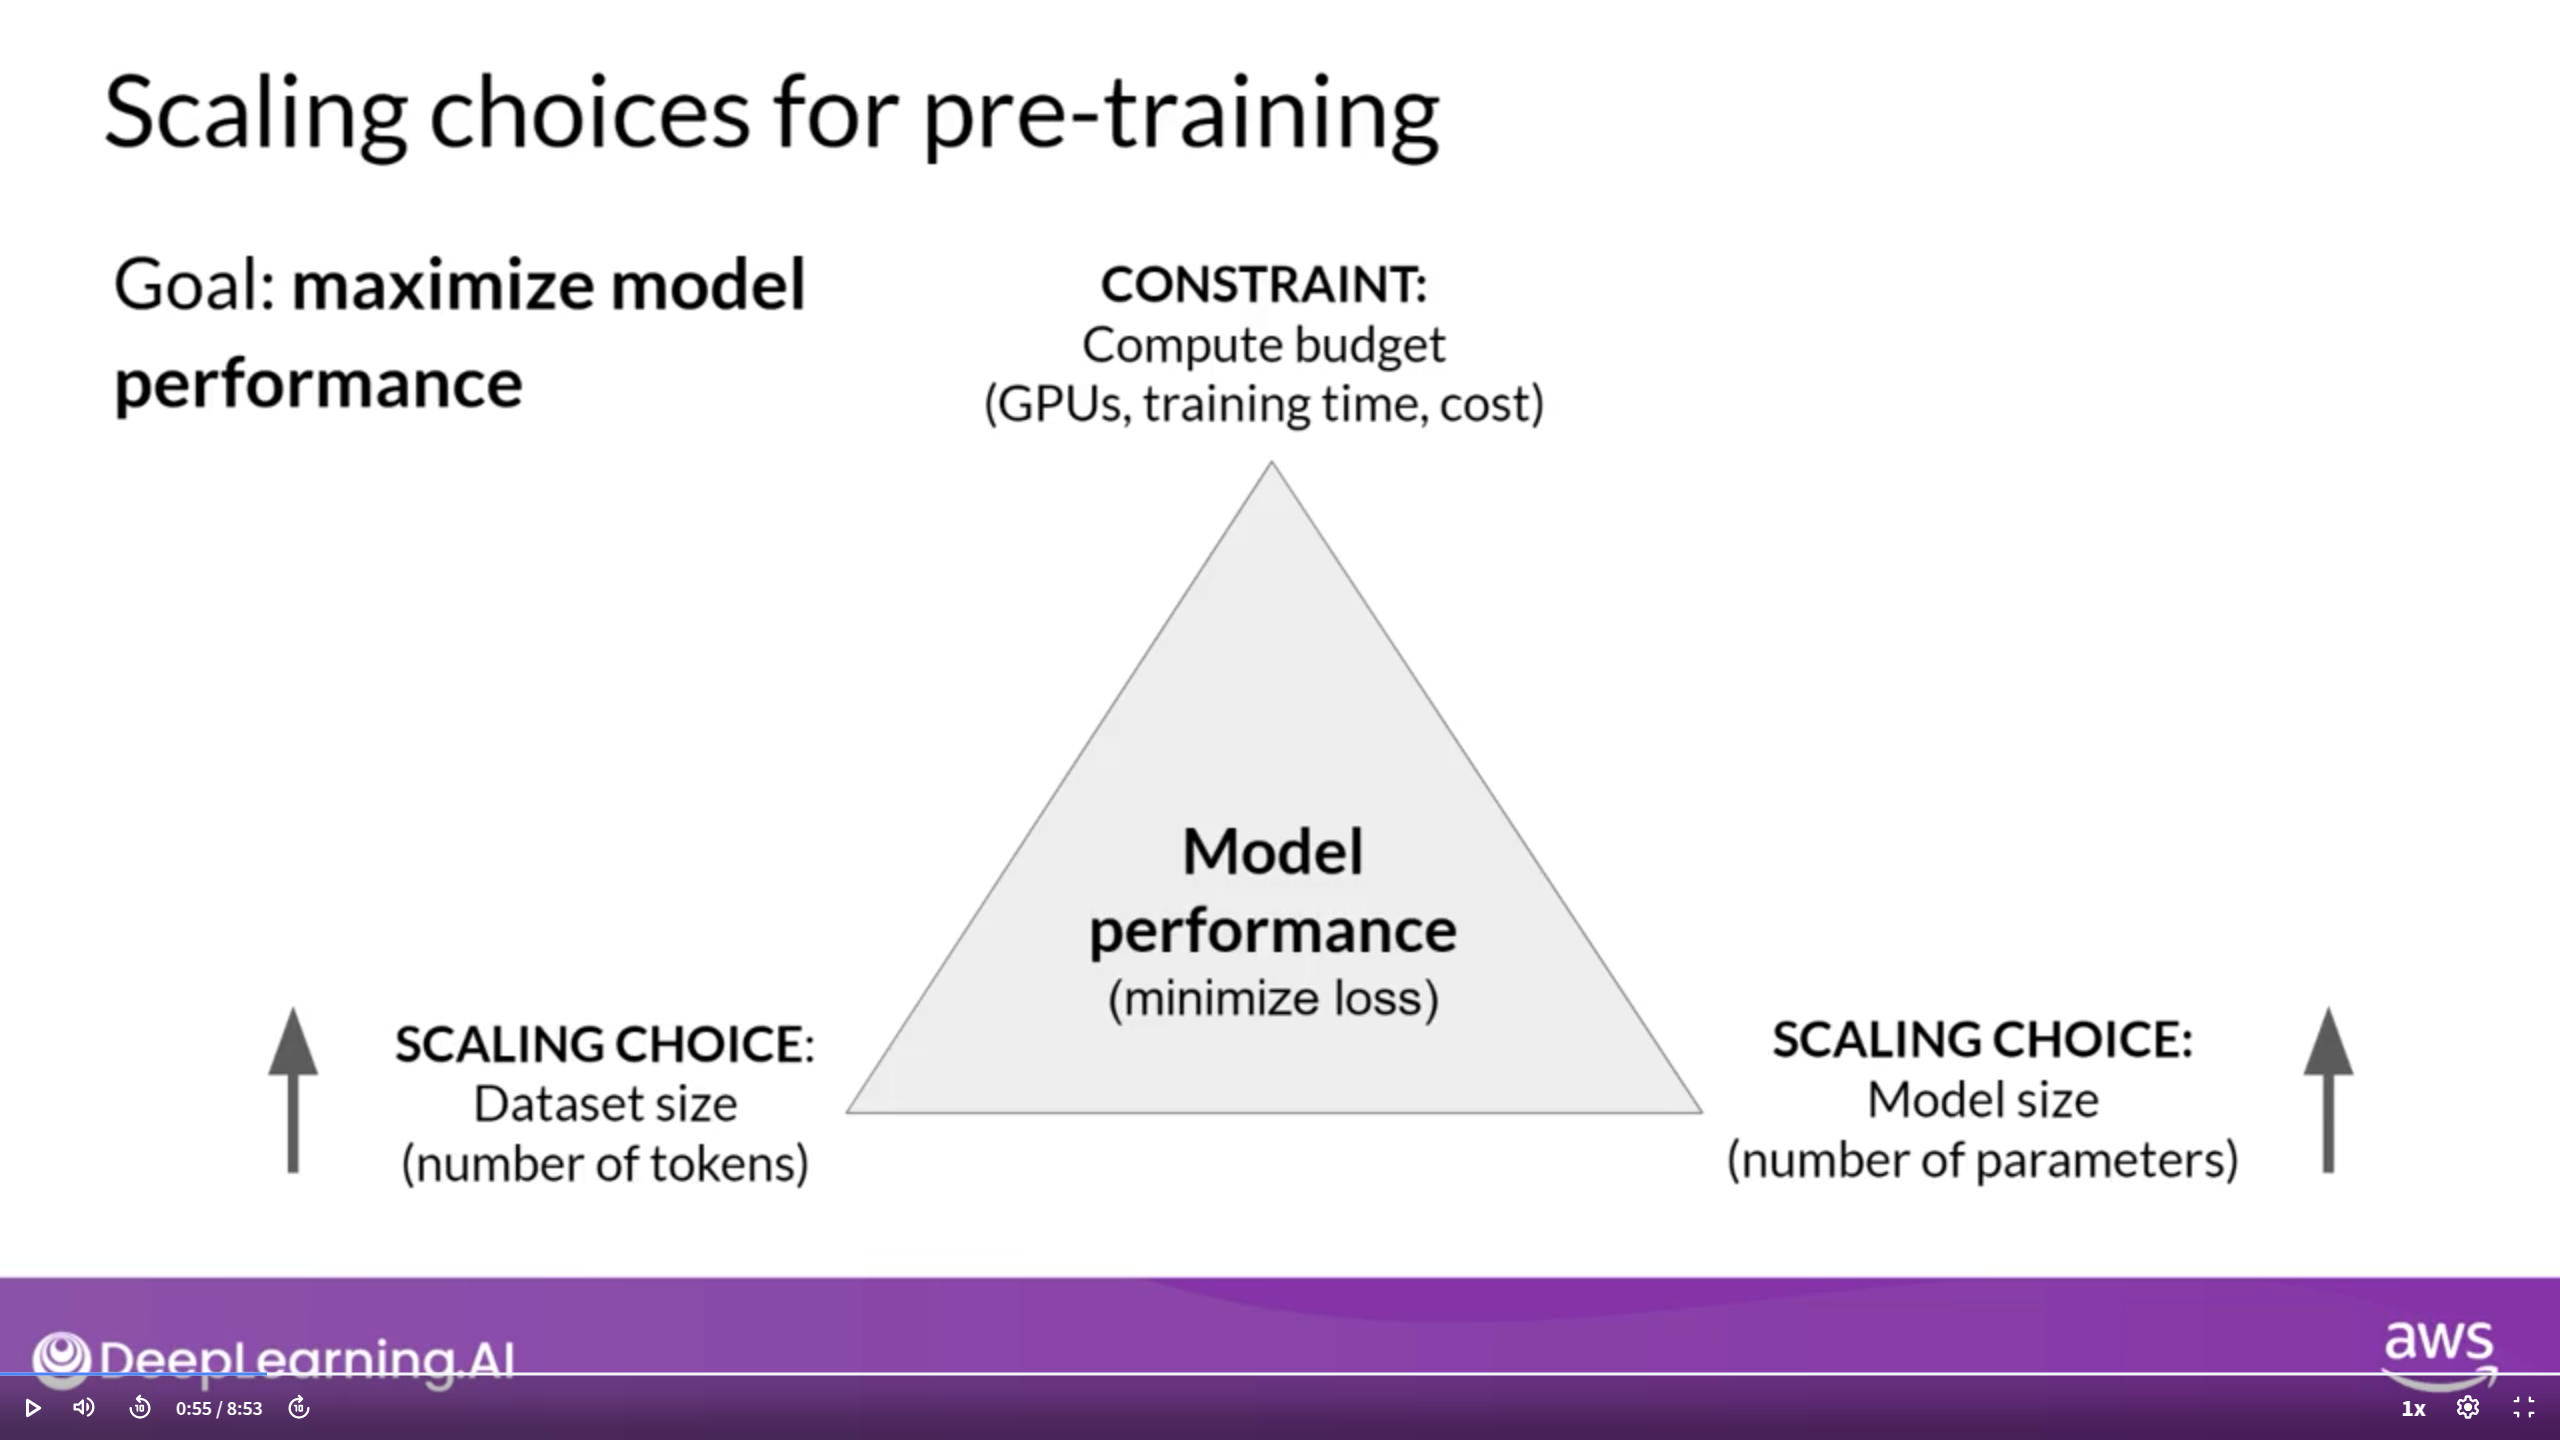
\includegraphics[trim=0cm 6cm 5cm 0cm,clip,scale=0.15]{pics/performance.png}
  %{\footnotesize\textbf{Notes:} XXX.} % changed <<<<<<<<<<
  %#\label{XXX}
\end{figure}

\section{Instruction fine-tuning}
How to fine-tune an LLM with instruction prompts? In the previous section, we learned how to use the few-shot method to improve the learning/output, but this method may not work for smaller models. More importantly, examples take up space in the context window. Instead, we can use fine-tuning to further tune a base model.
1:44

\chapter[Miscellaneous topics]{Miscellaneous topics}

\section{One hot encoding for categorical features}
\label{sec:one-hot}

\href{https://www.youtube.com/watch?v=v_4KWmkwmsU&ab_channel=deeplizard}{source1} and \href{https://machinelearningmastery.com/how-to-one-hot-encode-sequence-data-in-python/}{source2}

A categorical feature takes only a few limited number of values. There are tree options to deal with the categorical features:
\begin{itemize}
  \item Drop the feature: this option works only if the feature does not provide any useful information.
  \item Ordinal encoding: assigning a value to each category \textbf{(ordinal variables)}. This method works for tree-based (decision tree) models.
  \item One-hot encoding: creating one feature for each category, and assigning binary values. This method works particularly well if there is no clear ordering in the categorical data. We refer to categorical variables without an intrinsic ranking as \textbf{nominal variables}. One-hot encoding generally does not perform well if the categorical variable takes on a large number of values (15 and more). We refer to the number of unique entries of a categorical variable as the cardinality of that categorical variable. High cardinality columns can either be dropped from the dataset, or we can use ordinal encoding.
\end{itemize}

A one hot encoding is a representation of categorical features as binary vectors. This first requires that the categorical values be mapped to integer values. Then, each integer value is represented as a binary vector that is all zero values except the index of the integer, which is marked with a 1.

Example: assume we have a sequence of labels with the values \textit{red} and \textit{green}. We can assign \textit{red} an integer value of 0 and \textit{green} the integer value of 1. As long as we always assign these numbers to these labels, this is called an integer encoding. Consistency is important so that we can invert the encoding later and get labels back from integer values, such as in the case of making a prediction. Next, we can create a binary vector to represent each integer value. The vector will have a length of 2 for the 2 possible integer values. The \textit{red} label encoded as a 0 will be represented with a binary vector [1, 0] where the zeroth index is marked with a value of 1. In turn, the \textit{green} label encoded as a 1 will be represented with a binary vector [0, 1] where the first index is marked with a value of 1. If we had the sequence: \textit{red, red, green}, we could represent it with the integer encoding: 0, 0, 1. And the one hot encoding of:
[1, 0], [1, 0], and [0, 1].

Why Use a One Hot Encoding?
A one hot encoding allows the representation of categorical data to be more expressive. Many machine learning algorithms cannot work with categorical data directly. The categories must be converted into numbers. This is required for both input and output variables that are categorical. We could use an integer encoding directly, rescaled where needed. This may work for problems where there is a natural ordinal relationship between the categories, and in turn the integer values, such as labels for temperature \textit{cold, warm, and hot}.

There may be problems when there is no ordinal relationship and allowing the representation to lean on any such relationship might be damaging to learning to solve the problem. An example might be the labels dog and cat

In these cases, we would like to give the network more expressive power to learn a probability-like number for each possible label value. This can help in both making the problem easier for the network to model. When a one hot encoding is used for the output variable, it may offer a more nuanced set of predictions than a single label.

We can use libraries such is scikit-learn and keras to encode a categorical feature for ML.

\section{Evaluating the model-partitioning the data set}
\label{sec:dist}

Partition the data into three sets: training set, cross validation set (AKA validation/development/dev set), and test set. Train using the training set, but use the cost function with the cross validation set to evaluate the model (without the regularization parameter). To estimate the generalization error use the test set. The data allocation varies as the number of samples grows. For example, for smaller data set (< 10,000) 60\%/20\%/20\% is reasonable, but for very large data set (1,000,000), we can use 98/1/1.

The other way to evaluate a classification model is find the fraction of the test set and the fraction of the train set that the algorithm has mis-classified.

When selecting a model, you want to choose one that performs well both on the training and cross validation set. It implies that it is able to learn the patterns from your training set without overfitting. If you used the defaults in this lab, you will notice a sharp drop in cross validation error from the models with degree=1 to degree=2. This is followed by a relatively flat line up to degree=5. After that, however, the cross validation error is generally getting worse as you add more polynomial features. Given these, you can decide to use the model with the lowest cv\_mse as the one best suited for your application.

Mismatched train/test distribution: they should be of the same distribution. Choose the dev set and test set to reflect data you expect to get in the future and consider important to do well on. For example, if you training cat recognition models, and have 200K good images and 10K mobile images (the actual use-case distribution), it is not a good idea to merge all 210K images, shuffle, and split. The better option is to split the 10K mobile data into dev and test sets, each 2.5K, and add 5K mobile images to the good 200K images for training.

For the size of the test set, we need to set it such that it is big enough to give high confidence in the overall performance of your system. For some applications, we don't need to have test set, just train and dev is fine.




\section{Cross validation method}

The goal is always to generalize the model to fit the real world data. The test set is just a representation of the data that we may see in future. The model should be complex enough to model the training set without over-fitting.

The data points that we are using for training are assumed to be Independent and Identically Distributed (IID), which means that there’s no inherent difference between training, testing and real-world data and all the data is coming from the same source. This is the \textit{Fundamental Assumption of Supervised Learning.}


A fixed validation set leaves some random chance in determining model scores. That is, a model might do well on the fixed validation set, even if it would be inaccurate on a different set. The larger the validation set, the less randomness (aka \textit{noise}) there is in our measure of model quality, and the more reliable it will be. Unfortunately, we can only get a large validation set by removing rows from our training data, and smaller training datasets mean worse models! The idea is that we select part of the training set as the test set, not touching the actual test during the training set. This is indeed the cross validation set.

Cross Validation steps:

\begin{itemize}
  \item Randomly partition the training data into k folds of equal size.
  \item Train the model on all the folds except for one (k-1).
  \item Validate the model’s performance using the fold that was not used in training.
  \item Repeat steps 2 and 3 using different combinations of these folds.
  \item Average the error in predicting the polynomial trained on the training folds.
\end{itemize}

Cross-validation gives a more accurate measure of model quality, which is especially important if you are making a lot of modeling decisions. However, it can take longer to run, because it estimates multiple models (one for each fold). For small datasets, where extra computational burden isn't a big deal, you should run cross-validation. For larger datasets, a single validation set is sufficient. Your code will run faster, and you may have enough data that there's little need to re-use some of it for holdout. There's no simple threshold for what constitutes a large vs. small dataset. But if your model takes a couple minutes or less to run, it's probably worth switching to cross-validation. Alternatively, you can run cross-validation and see if the scores for each experiment seem close. If each experiment yields the same results, a single validation set is probably sufficient. Note that we no longer need to keep track of separate training and validation sets.

To use cross validation, it is more convenient to implement a pipeline.

Observation for using cross validation with linear regression:
\begin{itemize}
  \item Average cross validation error is higher than training error for lower orders .
  \item Average cross validation error decreases as the polynomial order increases (same for training error).
  \item After the golden degree, increasing the degree of polynomial will result in overfitting, and the Cross Validation error will start to increase.
\end{itemize}

\section{Accuracy of the model: F1 score, precision, and recall}
Refer to \href{https://scikit-learn.org/stable/auto_examples/model_selection/plot_precision_recall.html#precision-recall}{this source.}

Precision (P) is defined as the number of true positives ($T_p$) over the number of true positives plus the number of false positives ($F_p$): $P = \frac{T_p}{T_p + F_p} $. This criterion implies the percentage of true positive (of all examples that are positive, what percentage are actually positive). This means if ML detects a class/category, how likely it is correct.

Recall (R) is defined as the number of true positives ($T_p$) over the number of true positives plus the number of false negatives ($F_n$): $R = \frac{T_p}{T_p + F_n} $. This criterion implies what percentage of actual positives are correctly recognized. This means if ML can correctly identify the class even if the class is very rare.


\begin{figure}[H]
  \centering
  \includegraphics[trim =0.0cm 0.0cm 0.0cm 0.0cm, clip, scale=0.15]{pics/confusionMatrix.png}
  \caption{confusion matrix}
  %{\footnotesize\textbf{Notes:} XXX.} % changed <<<<<<<<<<
  %#\label{XXX}
\end{figure}


These quantities are also related to the ($F1$) score, which is defined as the harmonic mean of precision and recall: $F1 = 2 \frac{R * P}{ P + R } $. The F1 score can be interpreted as a harmonic mean of the precision and recall, where an F1 score reaches its best value at 1 and worst score at 0. F1 score allows us to select the best model among many models with different recall and precision. F1 combines both recall and precision.

The other important factor is the running time of the model. We can combine accuracy and running time into one metric. What we want is to maximize accuracy subject to running time less than a certain amount. In that sense, running time itself becomes an optimization metric. This metric is just a satisficing metric (should be less than a certain amount).

\section{Optimization}

\subsection{Cost function}
\label{sec:cost}
Loss function: Used when we refer to the error for a single training example. Cost function: Used to refer to an average of the loss functions over an entire training dataset.
The cost function gives you a way to measure the error, and how well a specific set of parameters fits the training data. Thereby gives you a way to try to choose better parameters. The selection of the loss function depends on the model.

Let's use the concept of multiple linear regression (which is the same for NN) to discuss the cost function.

Parameters/coefficients/weights of the model (In ML, parameters of a model are the variables that you can do training in order to improve the model):
\begin{equation}
  w_1, . . . , w_n , b \equiv \overrightarrow{w} ,b
\end{equation}

Here is the model:
\begin{equation}
	f_{\overrightarrow{w},b} (\overrightarrow{x}) = w_1x_1 +  ... + w_nx_n + b
\end{equation}

\begin{multline}
		\text{data points } \{(x_i, y_i): i=1 ... m \} \\
    \hat{y}^{(i)} = f_{\overrightarrow{w},b} (\overrightarrow{x}^{(i)})  = \overrightarrow{w} \overrightarrow{x} ^ {(i)} + b \\
\end{multline}

Problem statement: find $\overrightarrow{w},b$ such that $\hat{y}^{(i)}$ is close to $y^{(i)}$ for all $(x^{(i)}, y^{(i)} )$. $\big(\hat{y}^{(i)}  - y^{(i)} \big) ^2$, the error for one single sample is called the loss function.

To find $\overrightarrow{w},b$, we form the the cost function. The cost function depends on the method we measure the error. There are many methods to define loss/cost functions. One example is Mean Absolute Error (MAE), which measures the disparity from the true target by an absolute difference: abs(y\_true - y\_pred).

\begin{multline}
  \text{find $\overrightarrow{w},b$:} \\
  \text{minimize:  }  J(\overrightarrow{w},b) = \frac{1}{m} \sum_{i=1}^{m} \big(\hat{y}^{(i)}  - y^{(i)} \big) \\
\end{multline}


The other widely used method is \textbf{mean squared error cost (MSE)}:

\begin{multline}
	\text{find $\overrightarrow{w},b$:} \\
	\text{minimize:  }  J(\overrightarrow{w},b) = \frac{1}{2m} \sum_{i=1}^{m} \big(\hat{y}^{(i)}  - y^{(i)} \big) ^2 = \frac{1}{2m} \sum_{i=1}^{m} \big( wx ^ {(i)} + b - y^{(i)} \big) ^2 \\
\end{multline}
m is the to total number of data points. The extra 2 in the denominator is just for convenience. This is the squared error cost function, which is widely used. In sklearn, we can calculate the cost with mean\_squared\_error. However, there are other options for the cost functions as well. For example, the squared error cost function is not an ideal cost function for logistic regression, using Sigmoid function. The reason is that the logistic regression model, which is defined by (sigmoid):

\begin{equation}
  f_{\overrightarrow{w},b} (\overrightarrow{x}) = \frac{1}{1+e^{-(\overrightarrow{w} \overrightarrow{x} ^ {(i)} + b)}}
\end{equation}

is non-convex, as opposed to linear regression model which is convex. For logistic/classification problems, we cannot use Mean Absolute Error (MAE) either for the same reason. To have a convergent gradient descent method, the cost function should be convex.

\begin{figure}[htbp]
  \begin{center}
    \includegraphics[trim =0cm 6.0cm 0cm 20.0cm, clip, scale=0.15]{pics/logistic.png}
    \caption{cost function for logistic function}
    %\label{}
  \end{center}
\end{figure}

To convert the logistic function to a convex function (for a binary classification), we need to ue the following loss definition known as logistic loss. AKA binary cross entropy (see ML C1W3+ML C2W2). What we want instead is a distance between probabilities, and this is what cross-entropy provides. Cross-entropy is a sort of measure for the distance from one probability distribution to another. The idea is that we want our network to predict the correct class with probability 1.0. The further away the predicted probability is from 1.0, the greater will be the cross-entropy loss:

\begin{multline}
J(\overrightarrow{w},b) = \frac{1}{m} \sum_{i=1}^{m} \frac{1}{2}  L\big(\hat{y}^{(i)}  - y^{(i)} \big) = \frac{1}{m} \sum_{i=1}^{m} \frac{1}{2}  L\big(f_{\overrightarrow{w},b} (\overrightarrow{x}^{(i)})   - y^{(i)} \big)\\
L\big(f_{\overrightarrow{w},b} (\overrightarrow{x}^{(i)})   - y^{(i)} \big) =
\begin{cases}
  -log\big( f_{\overrightarrow{w},b} (\overrightarrow{x}^{(i)}) \big)  \;\; \text{if} \;\; y^{(i)} = 1  \\
  -log\big(1-f_{\overrightarrow{w},b} (\overrightarrow{x}^{(i)}) \big)  \;\; \text{if} \;\; y^{(i)} = 0  \\
\end{cases}
\end{multline}

If $y^{(i)} = 1$ then, if the predicted value $f_{\overrightarrow{w},b} (\overrightarrow{x}^{(i)}) $ is close to one, the loss function is close to zero (reduces the loss), but if the predicted value is close to zero, then the function penalize the loss function with a large number. The other way around for $y^{(i)} = 0$.

\begin{figure}[htbp]
  \begin{center}
    \includegraphics[trim =0cm 6.0cm 0cm 0.0cm, clip, scale=0.15]{pics/logistic2.png}
    \caption{cost function for logistic function}
    %\label{}
  \end{center}
\end{figure}

To simplify this loss and cost functions, we re-write it as follows:

\begin{multline}
L\big(f_{\overrightarrow{w},b} (\overrightarrow{x}^{(i)})   - y^{(i)} \big) = - y^{(i)} log\big( f_{\overrightarrow{w},b} (\overrightarrow{x}^{(i)}) \big) - (1-y^{(i)}) log\big(1-f_{\overrightarrow{w},b} (\overrightarrow{x}^{(i)}) \big) \\
J(\overrightarrow{w},b)   = -\frac{1}{m} \sum_{i=1}^{m} \big[ y^{(i)} log\big( f_{\overrightarrow{w},b} (\overrightarrow{x}^{(i)}) \big) + (1-y^{(i)}) log\big(1-f_{\overrightarrow{w},b} (\overrightarrow{x}^{(i)}) \big)  \big] \\
\end{multline}


Here is the summary of the steps for training any ML model (nn, linear regression, etc.-see code C2W1\_NN/2\_neuralNet.ipynb):
\begin{enumerate}
  \item \textit{Define model} by specify how to compute output given input x and parameters w, and b ($f_{\overrightarrow{w},b} (\overrightarrow{x})$).
  \item Specify \textit{Loss function} $L (f_{\overrightarrow{w},b} (\overrightarrow{x}) )  $ and \textit{cost function} $J(\overrightarrow{w},b) = \frac{1}{m} \sum_{i=1}^{m} \frac{1}{2}  L\big(f_{\overrightarrow{w},b} (\overrightarrow{x}^{(i)}) - y^{(i)} \big)$
  \item \textit{Train} on data to minimize $J(\overrightarrow{w},b)$, for example using gradient descent methods and back propagation.
\end{enumerate}

The same way, the loss function for softmax is:

\begin{equation}
  L\big( a_1, a_2, ..., a_m, y \big) =
  \begin{cases}
    -log ( a_1 )  \;\; \text{if} \;\; y = 1  \\
    -log ( a_2 )  \;\; \text{if} \;\; y = 2  \\
    \vdots\\
    -log ( a_m )  \;\; \text{if} \;\; y = m  \\
  \end{cases}
  \label{eq:softmaxLoss}
\end{equation}

Note in \ref{eq:softmaxLoss} above, only the line that corresponds to the target contributes to the loss, other lines are zero. To write the cost equation we need an 'indicator function' that will be 1 when the index matches the target and zero otherwise.
$$\mathbf{1}\{y == n\} = =\begin{cases}
  1, & \text{if $y==n$}.\\
  0, & \text{otherwise}.
\end{cases}$$
The cost is (called Sparse Ctegorical Cross Entropy)-SparseCtegoricalCrossentropy):
\begin{align}
  J(\mathbf{w},b) = - \left[ \sum_{i=1}^{m} \sum_{j=1}^{N}  1\left\{y^{(i)} == j\right\} \log \frac{e^{z^{(i)}_j}}{\sum_{k=1}^N e^{z^{(i)}_k} }\right] \tag{4}
\end{align}
where $m$ is the number of examples, $N$ is the number of outputs. This is the average of all the losses.





We can also add a weight to this error classification (\textbf{1}) to penalize some cases. For example, if we are training a cat classification model, and the model shows pornographic pics as cats, we can penalize the pornographic images with a larger weight. In that case, the error/cost would be:


\begin{align}
  J = \frac{1}{ \sum_{i = 1}^{m_{dev}} \mathbf{w^{(i)}} } \sum_{i = 1}^{m_{dev}} \mathbf{w^{(i)}} 1 \{y_{predic}^{(i)}  \neq y^{(i)} \}\\
  \mathbf{w^{(i)}} = \begin{cases}
    1, & \text{if} x^{(i)} \text{is non-porn} \\
    10, & \text{if} x^{(i)} \text{is porn}
  \end{cases}
\end{align}


The error model/cost function is orthogonal (separate problem) than the training and doing well on the metric itself. First, we need to establish the error/target, then we need to train the model to reduce the error.

For more accurate (less floating point error) calculation in tensorflow, it is preferred to have a linear activation function for the last layer, instead of a softmax (the output is this form call logits) use from\_logits=True. This informs the loss function that the softmax operation should be included in the loss calculation. This allows for an optimized implementation. Notice that in the preferred model, the outputs are not probabilities, but the output for each data sample is a vector of size the number of neurons in the last year. This vector for each sample can range from large negative numbers to large positive numbers. The output must be sent through a softmax when performing a prediction that expects a probability. However, we really don't need to apply a softmax to select the most likely category, we can just find the index of the largest output using np.argmax(). See 1\_MachineLearning\_Stanford\_Projects\_python\_C2W2\_2\_softmax.ipynb.



\subsection{Gradient descent (steepest descent) method}
\label{sec:gradient}

An optimization method to minimize any function. Depending on the initial starting point, the method may end up at a different local minimum. \\

Method: \\
For a cost function $J(\overrightarrow{w},b)$,  we want to find  $ \overrightarrow{w} (w_1, w_2, ...) , b$ to minimize $J$.\\

Algorithm: \\
\begin{itemize}
\item start with some initial $\overrightarrow{w}, b$.
\item update $w_j$ \textit{simultaneously} until the algorithm converges, meaning you reach a local minimum, where additional iteration does not change the point. It is incorrect to use new values of $w_j$  (j number of features) to update other parameters in the same iteration.
\begin{equation}
\begin{split}
  w_j =& w_j - \alpha \frac{\partial}{\partial w_j} J(\overrightarrow{w},b) \\
  b =& b - \alpha \frac{\partial  }{\partial b} J(\overrightarrow{w},b) \\
\end{split}
\end{equation}
\end{itemize}

The negative is because we want to move in the opposite direction. $\alpha$ is the learning rate (step size), see \ref{sec:learningRate}.

The derivatives of cost functions for regular regression and logistic regression are:
\begin{equation}
\label{eq:derivatives}
\begin{split}
\frac{\partial}{\partial w_j} J(\overrightarrow{w},b) =& \frac{1}{m} \sum_{i=1}^{m} \big(\hat{y}^{(i)} - y^{(i)} \big) x_j^{(i)} = \frac{1}{m} \sum_{i=1}^{m} \big( f_{\overrightarrow{w},b} (\overrightarrow{x}^{(i)}) - y^{(i)} \big) x_j^{(i)} \text{\: \: for each j} \\
\frac{\partial}{\partial b} J(\overrightarrow{w},b)   =& \frac{1}{m} \sum_{i=1}^{m} \big( f_{\overrightarrow{w},b} (\overrightarrow{x}^{(i)})  - y^{(i)} \big)
\end{split}
\end{equation}

But note that the definition of f for the two regressions are different (for logistic, f is the sigmoid function).

Back propagation is used to find the derivatives of cost function with respect to its parameters. This method is nothing but the chain rule. This method is cheaper (\#layers + \#parameter) compared to a direct calculation of the derivatives (\#layers $\times$ \#parameter). The idea is to use the chain rule from left to right.

Note that since the slope is close to zero at both ends of Sigmoid function, the gradient descent becomes very slow, but with ReLU, we don't have this issue.


\textbf{Vanishing /Exploding Gradients:}
For a deep NN, if activation units or weights are greater than one, they explode after multiplying in the forwared propagation. Conversely, if the weights are less than one, they vanish. This causes a very small training process/gradient descent. To solve this issue, we need to be very careful how we should initialize the weights, by setting the weight, not too much greater or smaller than one.

\textbf{\textit{Local optima in neural network}} most neural network problems are saddle points rather than local optima. Problem is really not the local optima, but the plateaus, a region where the derivative is close to zero for a long time.


\subsubsection{Various types of gradient descent:}
\textbf{\textit{Batch gradient descent:}} each step of gradient descent uses all the training examples. While this batching provides computation efficiency, it can still have a long processing time for large training datasets as it still needs to store all of the data into memory. Batch gradient descent also usually produces a stable error gradient and convergence (if you plot cost vs iteration, ideally it should decrease as the number of iteration increases), but sometimes that convergence point isn't the most ideal, finding the local minimum versus the global one.

\textbf{\textit{Mini-batch gradient descent}} updates the parameters using a subset of training samples. That means you do a full forward and backward propagation using a subset of samples. If you plot cost vs iterations, it is more noisy but the trend should be the same as a batch gradient descent. The noise is due to the subsets, one subset might have a higher cost, and the other might have a lower cost. The size of the mini-batch determines the type of gradient descent:

\begin{itemize}
  \item size = m: Batch gradient descent (The cons is that it is long per iteration. )
  \item size = 1: stochastic gradient descent (every example is its own mini-batch). This one is very noisy, but the average direction is toward the minimum, but may never hit the minimum.
  \item $1< size < m (~1000)$: This is the fastest learning. It makes progress without processing all training samples. Typical batch size is powers of two (64, 128, 256, 512, and 1024), depending on the memory size of GPU/CPU. The mini-batch size is another hyperparameter.
\end{itemize}

If the training set is small (less than 2000), go with the batch gradient method.

Epoch is a single pass through the training set. With Batch gradient descent, we do one step of the gradient descent in each epoch, but with the mini-batch gradient descent, we do as many as the number of mini batched gradient descent in each epoch.

\textbf{\textit{Gradient descent with momentum}}: It moves faster than the regular gradient descent. First, we need to learn about Exponentially weighted average, as defined below to find the average of a quantity, such as temperature.
\begin{equation}
  V_t = \beta V_{t-1} + (1-\beta) \theta_t
\end{equation}

$V_t$ is approximately average over $\frac{1}{1-\beta}$. The main advantage of this method, is that it takes a little memory, compared to a moving average that requires more memory (but it is more accurate).

The first few samples of the weighted average is not valid, because we don't have information for the prior points. We need to use bias computation to correct this. Bias correction makes the computation more accurately. The correction is:

\begin{equation}
  V_t = \frac{V_{t}}{1-\beta^t}
\end{equation}


Now that we know what exponential weighted average is, we need to use it with gradient descent to boost the efficiency. on iteration t, compute the dw and db as usual in the backward propagation, then:

\begin{align}
  V_{dw} &= V_{db} = 0 \\
  V_{dw} &= \beta V_{dw} + (1-\beta) dw \\
  V_{db} &=  \beta V_{db} + (1-\beta) db \\
  W &= W- \alpha V_{dw} \\
  b &= b- \alpha V_{db} \\
\end{align}

The $\beta$ is another hyperparameter in our model, but, in practice, it is ok to skip bias correction. Additionally, in some literature, the term $1-\beta$ is omitted.

\begin{figure}[htbp]
  \begin{center}
    \includegraphics[trim =25cm 22.0cm 40cm 20.0cm, clip, scale=0.4]{pics/GD_with_momentum.png}
    \caption{Gradient descent with momentum}
    %\label{}
  \end{center}
\end{figure}


\textbf{\textit{RMSprop (Root Mean Square propagation)}}:

on iteration t, compute the dw and db as usual in the backward propagation, then (squared in the following equation is element-wise):

\begin{align}
  S_{dw} &= S_{db} = 0 \\
  S_{dw} &= \beta S_{dw} + (1-\beta) dw^2\\
  S_{db} &= \beta S_{db} + (1-\beta) db^2\\
  W &= W- \alpha \frac{dw}{\sqrt{S_{dw}}} \\
  b &= b- \alpha \frac{db}{\sqrt{S_{db}}} \\
\end{align}


\textbf{\textit{Adam algorithm for optimization}}
Adam (Adaptive Moment estimation) is the same as the gradient descent method, but it adjusts the learning rate (increases or decreases the rate). In practice, this method uses different learning rates for different parameters. Basically, it is a combination of RMSprop and momentum.

The idea is that if gradient descent direction is roughly the same in each iteration, it increases the learning rate, but if direction is changing, the Adam algorithm reduces the learning rate.

on iteration t, compute the dw and db as usual in the backward propagation, then (squared in the following equation is element-wise):
\begin{align}
  S_{dw} &= S_{db} = V_{dw} = V_{db} = 0 \\
  V_{dw} &= \beta_1 V_{dw} + (1-\beta_1) dw \\
  V_{db} &=  \beta_1 V_{db} + (1-\beta_1) db \\
  S_{dw} &= \beta_2 S_{dw} + (1-\beta_2) dw^2\\
  S_{db} &= \beta_2 S_{db} + (1-\beta_2) db^2\\
  V_{dw}^{corrected} &= \frac{V_{dw}}{(1-\beta_1^t)} \\
  V_{db}^{corrected} &= \frac{V_{db}}{(1-\beta_1^t)} \\
  S_{dw}^{corrected} &= \frac{S_{dw}}{(1-\beta_1^t)} \\
  S_{db}^{corrected} &= \frac{S_{db}}{(1-\beta_1^t)} \\
  W &= W- \alpha \frac{V_{dw}^{corrected}}{\sqrt{S_{dw}^{corrected} + \epsilon}} \\
  b &= b- \alpha \frac{V_{db}^{corrected}}{\sqrt{S_{db}^{corrected} + \epsilon}} \\ \\
\end{align}

Hyperparameters are: $\alpha, \beta_1(0.9), \beta_2(0.999), \epsilon (10^{-8})$.

\subsection{Learning rate selection}
\label{sec:learningRate}
The choice of learning rate affects the efficiency of gradient descent. If the learning rate is too small, it would be very slow, and if it too large (overshoot), it may diverge. To start, we can set the learning rate to a very small number, and check if the cost function decreases with every single iteration. If not, there is bug in the code. We can plot the cost function (learning curve) with each iteration of the gradient descent. The learning rate $\alpha$ should be selected such that the cost function decreases as iterations increases. If this is not the case, then the learning rate is high. Generally, we need to test many learning rates and select the most optimized one.

If we are exactly at the minimum, since slope is zero, the value of the learning does not affect the results. Thus, even a fixed learning can reach the minimum.

\includegraphics[scale=0.12]{pics/LearningRate.png}

\includegraphics[scale=0.12]{pics/learningrate2.png}

\textbf{\textit{Learning rate decay}}: To speed up the learning algorithm, we can slowly reduce the learning rate over iterations. This helps with the mini-batched gradient descent, which potentially, has a noisy nature, and the algorithm may never reach to the minimum. By reducing the learning rate, we can reduce the region in which the algorithm is oscillating. Different formulas are used in the literature:

\begin{align}
  \alpha &= \frac{1}{1+decayRate\times epochNumber} \alpha_0 \\
  \alpha &= 0.95^{epochNumbre} \alpha_0 \; \; \text{(exponential decay)} \\
  \alpha &= \frac{k}{\sqrt{epochNum}}  \alpha_0 \\
  \text{staircase decay} \\
  \text{Manual decay}
\end{align}

Decay rate is another hyperparameter.

\section{Overfitting (high variance) vs underfitting (high bias)}
Overfitting (high variance) is the case that a model matches the training data almost perfectly, i.e.  $J_{train}$ is low, but does poorly in validation and other new data, i.e. $J_{cv}$ is high. On the flip side, When a model fails to capture important distinctions and patterns in the data, so it performs poorly even in training data, i.e. $J_{train}$ and $J_{cv}$ are high, that is called underfitting (high bias). Note that bias has a other meanings, such as checking the models based on characteristics such as gender, ethnicity, etc.

We can think of overfitting/underfitting as follows. the information in the training data as being of two kinds: signal and noise. The signal is the part that generalizes, the part that can help our model make predictions from new data. The noise is that part that is only true of the training data; the noise is all of the random fluctuation that comes from data in the real-world or all of the incidental, non-informative patterns that can't actually help the model make predictions. The noise is the part might look useful but really isn't. Now, the training loss will go down either when the model learns signal or when it learns noise. But the validation loss will go down only when the model learns signal. (Whatever noise the model learned from the training set won't generalize to new data.) So, when a model learns signal both curves go down, but when it learns noise a gap is created in the curves. The size of the gap tells you how much noise the model has learned. Underfitting the training set is when the loss is not as low as it could be because the model hasn't learned enough signal. Overfitting the training set is when the loss is not as low as it could be because the model learned too much noise. The trick to training deep learning models is finding the best balance between the two.




The case in the middle is "just right" model where $J_{train}$ and $J_{cv}$ are low.

\begin{figure}[H]
  \centering
  \caption{Bias vs Variance}
  \includegraphics[trim =0.0cm 0.0cm 0.0cm 0.0cm, clip, scale=0.12]{pics/biasVariance.png}
  %{\footnotesize\textbf{Notes:} XXX.} % changed <<<<<<<<<<
  %#\label{XXX}
\end{figure}

For some neural network applications, there are some cases where the model has the high bias and high variance at the same time.


Since we care about accuracy on new data, which we estimate from our validation data, we want to find the sweet spot between underfitting and overfitting, so that the model do well on examples that are not in the training set. This is called \textit{generalization}.

\textbf{To avoid underfitting:}
\begin{itemize}
\item adding new features: fixes high bias
\item adding polynomial features/bigger neural network fixes high bias (Wider networks have an easier time learning more linear relationships, while deeper networks prefer more nonlinear ones. Which is better just depends on the dataset.)
\item decreasing the regularization ($lambda$) fixes high bias
\end{itemize}

\textbf{To avoid overfitting:}
\begin{itemize}
\item one method is to collect more training data. If this option is available, probably we should try this first, but this is not always the option.
\item feature selection: review features, and use fewer features. The down side of this method is that we are throwing away some useful information about the model. See \ref{sec:featureEngineering}.
\item try getting additional features
\item try adding polynomial features $x_1^2, x_2^2, $ etc.
\item increasing regularization ($lambda$) fixes high variance. regularization: it gently reduces the impact of some features, without eliminating the feature. This, in some sort, means that we can have higher order parameters in the model, without overfitting. See \ref{sec:regularization}
\item Early stopping: the gap between the cross validation (dev) and training error decreases, until it grows at some point. We can stop once the gap between the dev and training error increases.
\end{itemize}


To add data, we can use the augmentation of data (rotating images, cropping images, distorting images, etc.). Data augmentation does not add a lot of information to our data set, but in case we really cannot get more data, we can use this method.  If there is not enough data to train a model, one option is to use the \textbf{\textit{transfer learning}}, in which you train a model using data from a different task (this step is called spervised pretraning), and fine tune the model with the actual data (this step is called fine tuning.). The other option is to use the other model parameters, and use the actual data to train only the last year of the neural network.

One more important topic is the baseline level of performance. In other words, how should one know if the $J_{train}$ is low, or high, or good enough. Once method to find the baseline performance is to compare the error with respect to the human-level performance. The other options are competing algorithm performance, or guess based on the past experience.

Note also that the best possible error is called Bayes optimal error. There is not a big difference between human-level and Bayes optimal error, thus, we can use the human-level error as a proxy for the Bayes error. In general, the training process is pretty fast, between until it reaches the human-level error, but slows down between the human-level and the Bayes. Knowing the human-level error, allows us to better analyze bias and variance.

If there is a gap between the baseline and the training error, then model in underfit (high bias), but if the gap is between the train and cross validation, it is the overfit (high variance) problem.


\begin{figure}[H]
  \centering
  \includegraphics[trim =0.0cm 0.0cm 0.0cm 0.0cm, clip, scale=0.12]{pics/biasVariance2.png}
  \caption{Bias vs Variance}
  %{\footnotesize\textbf{Notes:} XXX.} % changed <<<<<<<<<<
  %#\label{XXX}
\end{figure}


All the above argument is valid if the train and dev sets are from the same distribution. But if dev and training are from a different distribution. For example, if there is a gap between training and dev error (usually considered as high variance problem), the gap might be due to the difference in the dev set (dev set has more challenging samples). We mentioned in \ref{sec:dist} that the it is more efficient if the dev set contains samples from the real application (ex. mobile data), in that case, dev set has more difficult samples, compared to the training set which has high quality images/samples. The high dev set error is due to two items, one is the model has not seen this set before (new data which is the source of high variance), or second, the distribution gap issue (data mismatch problem). To detect the high dev set error is from which of these cases, we can define a new set call training-dev set, with the same distribution as the training set, but you did not trained on that. In short, we have four sets,  one: train, two: train-dev (both from the same distribution), three: dev, and four: test (3 and 4 from the same distribution but different from the first two sets). To do the error analysis, we get the error for all four sets. If there is a gap between train and train-dev (but little gap between train-dev and dev), this is an indication of the high variance problem. On the other hand, if train-dev error is only a bit above train, but has a good gap with the dev set, then the issue is data mismatch.


The other case is that if training, training-dev, dev, and test sets are close, but much higher than the human-level, this is an indication of the high bias problem.

Another note, it may also happen that dev/test set are much easier than the train and train-dev sets. In those cases, the error on dev/test might be even lower than the error in the train set.

\begin{figure}[H]
  \centering
  \includegraphics[trim =0.0cm 0.0cm 0.0cm 0.0cm, clip, scale=0.12]{pics/biasVariance_dist.png}
  \caption{Bias vs Variance distribution}
  %{\footnotesize\textbf{Notes:} XXX.} % changed <<<<<<<<<<
  %#\label{XXX}
\end{figure}

Here is the chart to decide how to adjust the model:

\begin{figure}[H]
  \centering
  \includegraphics[trim =0.0cm 0.0cm 0.0cm 0.0cm, clip, scale=0.12]{pics/biasVariance_chart.png}
  \caption{Bias vs Variance model based on error analysis}
  %{\footnotesize\textbf{Notes:} XXX.} % changed <<<<<<<<<<
  %#\label{XXX}
\end{figure}

To resolve a data mismatch, e can carry out manual error analysis to try to understand difference between training and dev/text sets. The other option is to make training data more similar or collect more data similar to dev/test sets. You can synthesis artificial data.

Note also that as the training set size increases, $J_{train}$ increases, because it is harder to fit the curve, but generally $J_{cv}$ drops.

\begin{figure}[H]
  \centering
  \includegraphics[trim =0.0cm 0.0cm 0.0cm 0.0cm, clip, scale=0.12]{pics/LearningCurve.png}
  \caption{learning curve}
  %{\footnotesize\textbf{Notes:} XXX.} % changed <<<<<<<<<<
  %#\label{XXX}
\end{figure}

For a model with high bias, the addition of sampling sizes after certain point, does not help with the performance.

\begin{figure}[H]
  \centering
  \includegraphics[trim =0.0cm 0.0cm 0.0cm 0.0cm, clip, scale=0.12]{pics/highBias.png}
  \caption{High bias}
  %{\footnotesize\textbf{Notes:} XXX.} % changed <<<<<<<<<<
  %#\label{XXX}
\end{figure}

For a model with high variance, increase the training set results in converging the errors to the baseline level.

\begin{figure}[H]
  \centering
  \includegraphics[trim =0.0cm 0.0cm 0.0cm 0.0cm, clip, scale=0.12]{pics/highVariance.png}
  \caption{High variance}
  %{\footnotesize\textbf{Notes:} XXX.} % changed <<<<<<<<<<
  %#\label{XXX}
\end{figure}

How does a neural network work in terms of bias and variance? Large neural networks are low bias machines, means, they generally fit the model. Using a bigger nn (more hidden layers or more units per layer) reduces the bias. A large neural network will usually do as well or better than a smaller one so long as reqularization is chosen appropriately. A larger neural network does not hurt, just more computationally intense. With neural network, the main problem is high variance rather than high bias.


\begin{figure}[H]
  \centering
  \includegraphics[trim =0.0cm 0.0cm 0.0cm 0.0cm, clip, scale=0.12]{pics/nn.png}
  \caption{Neural network training}
  %{\footnotesize\textbf{Notes:} XXX.} % changed <<<<<<<<<<
  %#\label{XXX}
\end{figure}

The other topic is orthogonalization. For training, we try to optimize the cost function, but at the same time, we want to avoid overfitting. These two items are orthogonal, and more optimization means more overfitting. Instead, we need a tool to mix these two goals.

\section{Transfer learning and multi-task learning}

It is the idea of taking the knowledge the neural network has learned from one task and apply that knowledge to a separate task. Based on this method, you train a network based on a data set, then, you re-train the last layer or even adding more layers, using the new data set.

Transfer learning makes sense when 1) both tasks/data have the same input, 2) when you have a lot of data for the data set you are transferring from, and less data for the set you are transferring to (It does not make sense for the other case (less data for the first set, more data for the second set)), and 3) low level features from the frist set coulld be helpful for learning the second set.

\begin{figure}[H]
  \centering
  \includegraphics[trim =0.0cm 0.0cm 0.0cm 0.0cm, clip, scale=0.12]{pics/transferLearning.png}
  \caption{Transfer learning}
  %{\footnotesize\textbf{Notes:} XXX.} % changed <<<<<<<<<<
  %#\label{XXX}
\end{figure}

In multi task learning, you start training an nn doing multiple tasks at the same time. In this manner, the final output layer has a dimension for all tasks. For example, if you are training an nn, to detect cars, pedestrians, and signs, then, the output layer should have three units, each for one class.

Multi-task learning makes sense when 1) training on a se of tasks that could benefit from having shared lower-level features, 2) amount of data you have for each task is quite similar.




\section{Regularization}
\label{sec:regularization}


\textbf{\textit{Lambda method}}
We need to modify the cost function by penalizing/regularize the features/parameters corresponding to over fitting. When there are many features for a model, it is prone to overfit. To avoid that, the idea is that to build a model with all features, because initially we don't know which features are important, but we penalize all features.

For a linear regression, we get (we are not penalizing b param, if we do it looks like this):

\begin{equation}
J(\overrightarrow{w},b) = \underbrace{  \frac{1}{2m} \sum_{i=1}^{m} \big( f_{\overrightarrow{w},b} (\overrightarrow{x}^{(i)}) - y^{(i)} \big) ^2}_\text{squared mean error} + \underbrace{ \frac{\lambda}{2m} \sum_{i=1}^n w_j^2 + \frac{\lambda}{2m} b^2}_\text{regularization term}
\end{equation}

This is the $L_2 (||w||^2_2) $ regularization, but we can also use the $L_1 (||w||_1)$ regularization.


The regularization for the neural network is applied to all weights:

\begin{equation}
  J(w^{[1]},b^{[1]}, ... , w^{[l]},b^{[l]}) = \frac{1}{m} \sum_{i=1}^{m} L \big( \hat{y}^{(i)} - y^{(i)} \big)+ \underbrace{ \frac{\lambda}{2m} \sum_{i=1}^l ||w^{[l]}||_F^2 }_\text{regularization term}
\end{equation}
where, the Frobenius norm is:

\begin{equation}
 ||w^{[l]}||_F^2 = \sum_{i=1}\sum_{j=1} (w_{ij}^{[l]})^2 \; \; w (n^{[l]} n^{[l-1]} )
\end{equation}


The regularization term forces the coefficient to remain small and $\lambda$ is the coefficient to control this. A large $\lambda$ results in underfit by reducing weights, but a very small one, leads to overfit. To find the right value for the regularization parameter, we can train the model with a sweep of $\lambda$ s and calculate $J_{cv}$ for each case, and pick a $\lambda$, corresponding to the lowest cost function. But this requires running the model many times for each regularization parameter.

\begin{figure}[H]
  \centering
  \includegraphics[trim =0.0cm 0.0cm 0.0cm 0.0cm, clip, scale=0.12]{pics/regularization.png}
  \caption{Regularization parameter}
  %{\footnotesize\textbf{Notes:} XXX.} % changed <<<<<<<<<<
  %#\label{XXX}
\end{figure}



Gradient descent with cost function (without b), looks like this (rewriting equation \ref{eq:derivatives}):
\begin{equation}
\label{eq:libRegReg}
  \begin{split}
    \frac{\partial}{\partial w_j} J(\overrightarrow{w},b) =&  \frac{1}{m} \sum_{i=1}^{m} \big( f_{\overrightarrow{w},b} (\overrightarrow{x}^{(i)}) - y^{(i)} \big) x_j^{(i)} + \overbrace{\frac{\lambda}{m} w_j}^\text{regularization term} \text{\: \: for each j} \\
    \frac{\partial}{\partial b} J(\overrightarrow{w},b)   =& \frac{1}{m} \sum_{i=1}^{m} \big( f_{\overrightarrow{w},b} (\overrightarrow{x}^{(i)})  - y^{(i)} \big)
  \end{split}
\end{equation}

For a logistic regression, we get:

\begin{equation}
  J(\overrightarrow{w},b)   = -\frac{1}{m} \sum_{i=1}^{m} \big[ y^{(i)} log\big( f_{\overrightarrow{w},b} (\overrightarrow{x}^{(i)}) \big) + (1-y^{(i)}) log\big(1-f_{\overrightarrow{w},b} (\overrightarrow{x}^{(i)}) \big)  \big]+ \underbrace{ \frac{\lambda}{2m} \sum_{i=1}^n w_j^2}_\text{regularization term}
\label{eq:logisticReg}
\end{equation}
The derivatives of equation \ref{eq:logisticReg} for gradient descent is similar to \ref{eq:libRegReg}, just f is different.


\textbf{\textit{Dropout regularization:}}

We set a probability to drop units in each layer of neural network. For each sample then we use the reduce network. To implement dropout, we can use the inverted dropout method. In each iteration, we randomly drop some units. There would be no dropout for predictions

\begin{figure}[H]
  \centering
  \includegraphics[trim =3.0cm 2.0cm 3.0cm 2.0cm, clip, scale=0.12]{pics/dropoutregularization.png}
  \caption{Neural network training}
  %{\footnotesize\textbf{Notes:} XXX.} % changed <<<<<<<<<<
  %#\label{XXX}
\end{figure}




\section{Model validation}

Always start with the dataset documentation.

In most (though not all) applications, the relevant measure of model quality is predictive accuracy. In other words, will the model's predictions be close to what actually happens.

There are many metrics for summarizing model quality, but we'll start with one called Mean Absolute Error (also called MAE). With the MAE metric, we take the absolute value of each error. This converts each error to a positive number. We then take the average of those absolute errors. This is our measure of model quality. sklearn has a function, mean\_absolute\_error, to calculate MAE.


Many people make a mistake when measuring predictive accuracy. They make predictions with their training data and compare those predictions to the target values in the training data. This is not valid. The most straightforward way to validate the model is to exclude some data from the model-building process, and then use those to test the model's accuracy on data it hasn't seen before. This data is called validation data.

\section{Data processing/cleaning: Missing Values}
\label{sec:missing}

Before we treat missing data, we need to know \textbf{Is this value missing because it wasn't recorded or because it doesn't exist?} If a value is missing because it doesn't exist (like the height of the oldest child of someone who doesn't have any children) then it doesn't make sense to try and guess what it might be. These values you probably do want to keep as NaN. On the other hand, if a value is missing because it wasn't recorded, then you can try to guess what it might have been based on the other values in that column and row.  There are many ways the data misses: wrong measurement, data is private, data is not available, etc.

Generally, there are three approaches deal with the missing data. These are quick and dirty approaches that probably remove some useful info or adding some noise to your dataset.
\begin{itemize}
  \item The simplest option: drop columns or features with missing values. Unless most values in the dropped columns are missing, the model loses access to a lot of (potentially useful!) information with this approach.
  \item Imputation: fills in the missing values with some number. For instance, we can fill in the mean value along each column, or we can choose the most popular data for the missing item. We can also assign the probability of each value of the attribute to the missing entries. The imputed value won't be exactly right in most cases, but it usually leads to more accurate models than you would get from dropping the column entirely.
  \item Extending imputation: we impute the missing values, as before. And, additionally, for each column with missing entries in the original dataset, we add a new column that shows the location of the imputed entries. For example, if the size of bedroom is missing for some instances, we add a new column, missing\_bedromm\_size, and set it to FALSE for all valid instances and TRUE for all missing instances. This will meaningfully improve results. In other cases, it doesn't help at all.
\end{itemize}

In pandas, we can use .isnul() to detect columns with missing data. We can use .drop to drop columns. We can also use dropna to either drop columns or instances.

\section{Data processing \& Feature engineering}
\label{sec:featureEngineering}

\subsection{Feature engineering}
The goal of feature engineering is simply to make your data better suited to the problem at hand. You might perform feature engineering to:
\begin{itemize}
  \item improve a model's predictive performance
  \item reduce computational or data needs
  \item improve interpretability of the results
\end{itemize}

Feature engineering is possible through:
\begin{itemize}
  \item determine which features are the most important with mutual information
  \item invent new features in several real-world problem domains (e.g. square the length of land, to get area, which is a more reasonable feature. It can predicate parabola now.)
  \item encode high-cardinality categoricals with a target encoding
  \item create segmentation features with k-means clustering
  \item decompose a dataset's variation into features with principal component analysis
\end{itemize}

A great first step is to construct a ranking with a feature utility metric, a function measuring associations between a feature and the target. Then you can choose a smaller set of the most useful features to develop initially and have more confidence that your time will be well spent. The metric we'll use is called "mutual information". It can \textbf{detect any kind of relationship, while correlation only detects linear relationships.} The mutual information (MI) between two quantities is a measure of the extent to which knowledge of one quantity reduces uncertainty about the other. Mutual Info varies between 0 (independent quantities) to $+ \infty $. It is a logarithmic func, and barely reaches to 2. It's possible for a feature to be very informative when interacting with other features, but not so informative all alone. MI can't detect interactions between features. It is a univariate metric.
The actual usefulness of a feature depends on the model you use it with. A feature is only useful to the extent that its relationship with the target is one your model can learn.

Scikit-learn has two mutual information metrics in its feature\_selection module: one for real-valued targets (mutual\_info\_regression) and one for categorical targets (mutual\_info\_classification).

\subsection{How to create new features}

\subsubsection{Mathematical transform}
Use arithmetic operations to create new features based on other features. For example, find the area of land by multiplying width by length. This will create non-linearity in the date.

For the neural network, you don't need to create non-linear features. Neural networks can learn non-linear relationships between the inputs and outputs. But for linear regression, you need to create non-linear features to capture non-linear relationships between the inputs and outputs.


\subsubsection{Count}
Features describing the presence or absence of something often come in sets, the set of risk factors for a disease, say. You can aggregate such features by creating a count. These features will be binary (1 for Present, 0 for Absent) or boolean (True or False). In Python, booleans can be added up just as if they were integers.

Example:

accidents["RoadwayFeatures"] = accidents[roadwayFeatures].sum(axis=1)

\subsubsection{Building up and breaking down features}
Add or breakdown strings to create new features. For example, break down phone numbers to area codes.

\subsubsection{Clustering}
Use, for example, K-means to cluster data points and add it as a feature. It requires a knowledge about the domain.


\subsubsection{Principal Component Analysis (PCA)}
There are two ways you could use PCA for feature engineering.

\begin{itemize}
  \item The first way is to use it as a descriptive technique. Since the components tell you about the variation, you could compute the MI scores for the components and see what kind of variation is most predictive of your target. That could give you ideas for kinds of features to create.
  \item The second way is to use the components themselves as features. Because the components expose the variational structure of the data directly, they can often be more informative than the original features. Here are some use-cases:
  \begin{itemize}
    \item Dimensionality reduction: When your features are highly redundant (multicollinear, specifically), PCA will partition out the redundancy into one or more near-zero variance components, which you can then drop since they will contain little or no information.
    \item Anomaly detection: Unusual variation, not apparent from the original features, will often show up in the low-variance components. These components could be highly informative in an anomaly or outlier detection task.
    \item Noise reduction: A collection of sensor readings will often share some common background noise. PCA can sometimes collect the (informative) signal into a smaller number of features while leaving the noise alone, thus boosting the signal-to-noise ratio.
    \item Decorrelation: Some ML algorithms struggle with highly-correlated features. PCA transforms correlated features into uncorrelated components, which could be easier for your algorithm to work with.
  \end{itemize}
\end{itemize}

PCA basically gives you direct access to the correlational structure of your data. You'll no doubt come up with applications of your own!

PCA Best Practices- there are a few things to keep in mind when applying PCA:
\begin{itemize}
\item PCA only works with numeric features, like continuous quantities or counts.
\item PCA is sensitive to scale. It's good practice to standardize your data before applying PCA, unless you know you have good reason not to.
\item Consider removing or constraining outliers, since they can have an undue influence on the results.
\end{itemize}


\subsubsection{Target Encoding}

This method, as opposed to all other methods, targets categorical features. It is similar to one-hot or label encoding, with the difference that it also uses the target to create the encoding. This makes it what we call a supervised feature engineering technique.

A target encoding is any kind of encoding that replaces a feature's categories with some number derived from the target. For example, \textit{mean encoding}, takes the average of the numerical target based on a categorical feature (ex. average/mean price of a car brand (make)). \textbf{Bin counting} is the equivalent encoded feature applied to a binary target.


Target encoding is great for:
\begin{itemize}
  \item High-cardinality features: A feature with a large number of categories can be troublesome to encode: a one-hot encoding would generate too many features and alternatives, like a label encoding, might not be appropriate for that feature. A target encoding derives numbers for the categories using the feature's most important property: its relationship with the target.
  \item Domain-motivated features: From prior experience, you might suspect that a categorical feature should be important even if it scored poorly with a feature metric. A target encoding can help reveal a feature's true informativeness.
\end{itemize}



There are at least two concerns with the target encoding:
\begin{itemize}
  \item unknown categories: Target encodings create a special risk of overfitting, which means they need to be trained on an independent "encoding" split. When you join the encoding to future splits, Pandas will fill in missing values for any categories not present in the encoding split. These missing values you would have to impute somehow.
  \item rare categories: When a category only occurs a few times in the dataset, any statistics calculated on its group are unlikely to be very accurate.
\end{itemize}

A solution to these problems are \textbf{smoothing}. The idea is to blend the in-category average with the overall average. Rare categories get less weight on their category average, while missing categories just get the overall average.

In pseudocode: encoding = weight * in\_category (ex. mean of the category for that feature) + (1 - weight) * overall (ex. mean of all categories for that feature). Where weight is a value between 0 and 1 calculated from the category frequency. An easy way to determine the value for weight is to compute an m-estimate: weight = n / (n + m), where n is the total number of times that category occurs in the data. The parameter m determines the "smoothing factor". Larger values of m put more weight on the overall estimate. When choosing a value for m, consider how noisy you expect the categories to be. Does the price of a vehicle vary a great deal within each make? Would you need a lot of data to get good estimates? If so, it could be better to choose a larger value for m; if the average price for each make were relatively stable, a smaller value could be okay.

\subsection{Scaling vs normalization}

In both cases, you're transforming the values of numeric variables so that the transformed data points have specific helpful properties to speed of the training. The point is to help with the gradient descent to converge faster. The difference is that: in \textbf{scaling}, you're changing the range of your data, while in \textbf{normalization}, you're changing the shape of the distribution of your data.

\subsubsection{scaling}
This means that you're transforming your data so that it fits within a specific scale, like 0-100 or 0-1. You want to scale data when you're using methods based on measures of how far apart data points are, like support vector machines (SVM) or k-nearest neighbors (KNN). With these algorithms, a change of "1" in any numeric feature is given the same importance. By scaling your variables, you can help compare different variables on equal footing.

\subsubsection{normalization}
Scaling just changes the range of your data. Normalization is a more radical transformation. The point of normalization is to change your observations so that they can be described as a normal distribution.

In general, you'll normalize your data if you're going to be using a machine learning or statistics technique that assumes your data is normally distributed. Some examples of these include linear discriminant analysis (LDA) and Gaussian naive Bayes. (Pro tip: any method with "Gaussian" in the name probably assumes normality.)

\subsection{Scaling a feature}
Having two features with large and small values may have adverse impact on our training. For example, for regression, it may cause large round off error, or affects the shape of gradient descent contours and as a result may cause slow convergence or even divergence. To avoid that, it is recommended to scale features so that they have the same range. After scaling, the data range would be 0 to 1.

\includegraphics[scale=0.12]{pics/scalingforGD.png}

\subsection{Mean normalization}
In this method, we first find the average of the feature ($\mu$). Each item of the feature is normalized as:
\begin{equation}
  x_i = \frac{x_i-\mu}{max-min}
\end{equation}

Then, we have the range for each feature between -1 and 1.

\subsection{z-score normalization}
In this method, we first find the standard deviation ($\sigma$) and the average ($\mu$) of the feature. Each item of the feature is normalized as:
\begin{equation}
  x_i = \frac{x_i-\mu}{\sigma}
\end{equation}

Then, we have the range for each feature between -1 and 1.
If you partition the set to training, cross validation, and testing sets, and z-score normalize training, you need to normalize testing and cross validation sets with the mean and variance of the training set to ensure that your input features are transformed as expected by the model.


\subsection{Combining features}
Using intuition to design new features by transforming or combining original features.


\subsection{Batch normalization}

This is the normalization of the activation units $a^{[l-1]}$ to help optimizing $W^{[l]}$ and $b^{[l]}$ in the next layer more efficiently. In the literature, we can apply normalization on $Z^{[l-1]}$ (before applying the activation function) or on $a^{[l-1]}$ (after applying the activation function). The former is more often. The normalization equation is the same as z-score normalization. $\epsilon$ is to avoid division by zero.

\begin{equation}
  z_{norm}^{(i)} = \frac{z^{(i)}-\mu}{ \sqrt{\sigma^2 + \epsilon}}
\end{equation}

We don't want all the hidden units have the mean zero and variance one to take advantage of the non-linearity of the model, especially with the sigmoid function, so to avoid that, we adjust the equation as follows:

\begin{equation}
  \tilde{Z}^{(i)} = \gamma  z_{norm}^{(i)}  + \beta
\end{equation}

where $\gamma$ and $\beta$ are learnable parameters (not hyperparameters) that can be optimized in each iteration, for example, using gradient descent.

This is how the batch norm is applied in a neural network:

\begin{figure}[H]
  \centering
  \includegraphics[trim =0.0cm 0.0cm 0.0cm 0.0cm, clip, scale=0.12]{pics/batchNorm.png}
  \caption{Batch normalization}
  %{\footnotesize\textbf{Notes:} XXX.} % changed <<<<<<<<<<
  %#\label{XXX}
\end{figure}

If we use batch norm with mini-batch, we can eliminate the b parameter, because it will be zeroed by the batch norm process anyways.

Here is the implementation of the nn with gradient descent (similarly for GD with momentum, RMSprop, Adam) with batch norm:

\begin{figure}[H]
  \centering
  \includegraphics[trim =0.0cm 0.0cm 0.0cm 0.0cm, clip, scale=0.12]{pics/NN_with_batchNorm.png}
  \caption{NN with Batch normalization}
  %{\footnotesize\textbf{Notes:} XXX.} % changed <<<<<<<<<<
  %#\label{XXX}
\end{figure}

One other impact that batch norm has in the training of a neural network is that it makes weights later or deeper in the nn more robust to changes to weights in earlier layers of the neural network. This is called covariant shift. This has some regularization effect.


\section{Ensemble methods}
Ensemble methods combine the predictions of several models (e.g., several trees, in the case of random forests).

\subsection{Gradient Boosting}
Gradient boosting is a method that goes through cycles to iteratively add models into an ensemble.

It begins by initializing the ensemble with a single model, whose predictions can be pretty naive. (Even if its predictions are wildly inaccurate, subsequent additions to the ensemble will address those errors.)

Then, we start the cycle:
\begin{itemize}
  \item First, we use the current ensemble to generate predictions for each observation in the dataset. To make a prediction, we add the predictions from all models in the ensemble.
  \item These predictions are used to calculate a loss function (like mean squared error, for instance).
  \item Then, we use the loss function to fit a new model that will be added to the ensemble. Specifically, we determine model parameters so that adding this new model to the ensemble will reduce the loss. (Side note: The "gradient" in "gradient boosting" refers to the fact that we'll use gradient descent on the loss function to determine the parameters in this new model.)
  \item Finally, we add the new model to ensemble,
  \item repeat!
\end{itemize}

XGBoost stands for extreme gradient boosting, which is an implementation of gradient boosting with several additional features focused on performance and speed. (Scikit-learn has another version of gradient boosting, but XGBoost has some technical advantages.) scikit-learn API for XGBoost (xgboost.XGBRegressor) allows us to build and fit a model just as we would in scikit-learn. The XGBRegressor class has many tunable parameters. See the code.


\subsection{Data leakage}

Data leakage (or leakage) happens when your training data contains information about the target, but similar data will not be available when the model is used for prediction. This leads to high performance on the training set (and possibly even the validation data), but the model will perform poorly in production.

In other words, leakage causes a model to look accurate until you start making decisions with the model, and then the model becomes very inaccurate.

There are two main types of leakage: target leakage and train-test contamination.

\textbf{Target leakage} occurs when your predictors include data that will not be available at the time you make predictions. It is important to think about target leakage in terms of the timing or chronological order that data becomes available, not merely whether a feature helps make good predictions.

Example: People take antibiotic medicines after getting pneumonia in order to recover. The raw data shows a strong  relationship between those columns, but \textit{took antibiotic medicine} is frequently changed after the value for \textit{got pneumonia} is determined. This is target leakage. Since validation data comes from the same source as training data, the pattern will repeat itself in validation, and the model will have great validation (or cross-validation) scores. But the model will be very inaccurate when subsequently deployed in the real world, because even patients who will get pneumonia won't have received antibiotics yet when we need to make predictions about their future health.

\textit{To prevent this type of data leakage, any variable updated (or created) after the target value is realized should be excluded.}

\textbf{Train-Test Contamination}
A different type of leak occurs when you aren't careful to distinguish training data from validation data.

Recall that validation is meant to be a measure of how the model does on data that it hasn't considered before. You can corrupt this process in subtle ways if the validation data affects the preprocessing behavior. This is sometimes called train-test contamination.

For example, imagine you run preprocessing (like fitting an imputer for missing values) before calling train\_test\_split(). The end result? Your model may get good validation scores, giving you great confidence in it, but perform poorly when you deploy it to make decisions.

After all, you incorporated data from the validation or test data into how you make predictions, so the may do well on that particular data even if it can't generalize to new data. This problem becomes even more subtle (and more dangerous) when you do more complex feature engineering.

As we discussed in the tutorial, to avoid overfitting, we need to fit the encoder on data heldout from the training set.

If your validation is based on a simple train-test split, exclude the validation data from any type of fitting, including the fitting of preprocessing steps. This is easier if you use scikit-learn pipelines. When using cross-validation, it's even more critical that you do your preprocessing inside the pipeline!


\section{Python}
\begin{itemize}
\item Use vectorization in python to improve the performance (for example: np.dot(W,x)).
\item To expand the dimension of a numpy array: np.expand\_dims(x, axis=1). This will convert (dim,) to (dim,1). For the reverse action, i.e. converting (dim,1) to (dim,), array[:,0].
\end{itemize}



\section{ML Checklist}

\begin{itemize}
  \item Inspect all features, look for duplicate features.
  \item Manage missing data (drop items with missing target, and impute missing items).
  \item Manage categorical/object features (cordinal, one-hot, etc.)
\end{itemize}
\subsection{Time series}

\begin{itemize}
  \item Plot lags to find seasonality/cycles and calculate correlation, and add new lag features if there is a high correlation.
  \item Plot partial autocorrelation, and add new lag features if there is a high correlation.
\end{itemize}


\section{Time series}
The basic object of forecasting is the time series, which is a set of observations recorded over time. In forecasting applications, the observations are typically recorded with a regular frequency, like daily or monthly.

One of the main forecasting approaches is the Linear regression method for forecasting (target = weight\_1 * feature\_1 + weight\_2 * feature\_2 + bias). But, first we need to generate the features corresponding to the time series. There are three kinds of features unique to time series: time-step features and lag features.

\textbf{Time-step features} are features we can derive directly from the time index. The most basic time-step feature is the time dummy, which counts off time steps in the series from beginning to end. Time-step features let you model time dependence. A series is time dependent if its values can be predicted from the time they occurred.

\textbf{Lag (and lead) features} are the second types of features that we can generate from the time series. To make a lag feature, we shift the observations of the target series so that they appear to have occurred later in time. Lag features let you model \textit{serial dependence}. A time series has serial dependence when an observation can be predicted from previous observations. \textbf{Adapting machine learning algorithms to time series problems is largely about feature engineering with the time index and lags.}


\textbf{Seasonal features} such as seasonal \textit{indicators} or Fourier transform features (will be discussed later).

There are three patterns/components of dependence in a time series:

Series = \textbf{trend }(moving average or linear regression (with different polynomial order) with time-step feature) + \textbf{seasonality} (weekly, monthly, etc. using indicator features (for short seasons) or Fourier method (if season is longer)) + \textbf{cycles} (serial dependence using lag feature) + \textbf{error}. Each of these items is called a component.

The residuals of a model are the difference between the target the model was trained on and the predictions the model makes -- the difference between the actual curve and the fitted curve, in other words.


Trend, seasonality, and cycles will be discussed next.

\subsection{Trend}
This portion of the time series can be captured by moving average rolling windows, or using linear regressions with the time-step feature. The trend models we learned about in this lesson turn out to be useful for a number of reasons. Besides acting as a baseline or starting point for more sophisticated models, we can also use them as a component in a "hybrid model" with algorithms unable to learn trends (like XGBoost and random forests).

\subsection{Seasonality}
We say that a time series exhibits seasonality whenever there is a regular, periodic change in the mean of the series. Seasonal changes generally follow the clock and calendar -- repetitions over a day, a week, or a year are common.

There are two kinds of features that model seasonality. The first kind, \textit{indicators}, is best for a season with few observations, like a weekly season of daily observations (7 observation in the season). The second kind, \textit{Fourier features}, is best for a season with many observations, like an annual season of daily observations (365 observations per season).

we can use a seasonal plot to discover seasonal patterns. A seasonal plot shows segments of the time series plotted against some common period, the period being the "season" you want to observe.


\subsubsection{Seasonal indicators}
A seasonal plot shows segments of the time series plotted against some common period, the period being the "season" you want to observe. Seasonal indicators are binary features that represent seasonal differences in the level of a time series. Seasonal indicators are what you get if you treat a seasonal period as a categorical feature and apply one-hot encoding. For example, by one-hot encoding days of the week, we get weekly seasonal indicators. Creating weekly indicators for the Trigonometry series will then give us six new "dummy" features. (Linear regression works best if you drop one of the indicators; we chose Monday in the frame below. This means the in the one-hot model, if all Tue ~ Sun is 0, it is Monday.)

\begin{figure}[htbp]
  \begin{center}
    \includegraphics[trim =30cm 8.0cm 20cm 27cm, clip, scale=0.4]{pics/seasonal_indicator.png}
    \caption{seasonal indicators}
    %\label{}
  \end{center}
\end{figure}

\subsubsection{Fourier features and periodogram}

The kind of feature we discuss now are better suited for long seasons over many observations where indicators would be impractical. Instead of creating a feature for each date, Fourier features try to capture the overall shape of the seasonal curve with just a few features. It is these frequencies within a season that we attempt to capture with Fourier features. The idea is to include in our training data periodic curves having the same frequencies as the season we are trying to model. Fourier features are pairs of sine and cosine curves, one pair for each potential frequency in the season starting with the longest. Fourier pairs modeling annual seasonality would have frequencies: once per year, twice per year, three times per year, and so on.

\begin{figure}[htbp]
  \begin{center}
    \includegraphics[trim =30cm 10.0cm 20cm 15cm, clip, scale=0.4]{pics/fourier.png}
    \caption{Fourier features}
    \label{default}
  \end{center}
\end{figure}

If we add a set of these sine / cosine curves to our training data, the linear regression algorithm will figure out the weights that will fit the seasonal component in the target series. The figure illustrates how linear regression used four Fourier pairs to model the annual seasonality in the Wiki Trigonometry series.

\begin{figure}[htbp]
  \begin{center}
    \includegraphics[trim =30cm 10.0cm 20cm 11cm, clip, scale=0.4]{pics/curves.png}
    \caption{Fourier features}
    %\label{default}
  \end{center}
\end{figure}

Notice that we only needed eight features (four sine / cosine pairs) to get a good estimate of the annual seasonality. Compare this to the seasonal indicator method which would have required hundreds of features (one for each day of the year). By modeling only the "main effect" of the seasonality with Fourier features, you'll usually need to add far fewer features to your training data, which means reduced computation time and less risk of overfitting.

\subsubsection{Choosing Fourier features with the Periodogram:}

How many Fourier pairs should we actually include in our feature set? We can answer this question with the periodogram. The periodogram tells you the strength of the frequencies in a time series. Specifically, the value on the y-axis of the graph is (a ** 2 + b ** 2) / 2, where a and b are the coefficients of the sine and cosine at that frequency (as in the Fourier Components plot above).

Removing from a series its trend or seasons is called \textbf{detrending} or \textbf{deseasonalizing} the series.

Once Fourier or seasonal indicator features created, we can use the linear (nonlinear/polynomial) regression for forecasting.


\subsection{Cycles: serial dependence (time series as features)}
Some time series, have \textit{time dependent properties}, that is, we could derive the feature directly from the time index (for example, weekly dependence). However, some other time series properties can only be modeled as serially dependent properties, that is, using as features past values of the target series. Plotted against past values (with lag) reveals the structure.

\subsubsection{Cycles} One especially common way for serial dependence to manifest is in cycles. Cycles are patterns of growth and decay in a time series associated with how the value in a series at one time depends on values at previous times, but not necessarily on the time step itself. Cyclic behavior is characteristic of systems that can affect themselves or whose reactions persist over time. Economies, epidemics, animal populations, volcano eruptions, and similar natural phenomena often display cyclic behavior. What distinguishes cyclic behavior from seasonality is that cycles are not necessarily time dependent, as seasons are. What happens in a cycle is less about the particular date of occurrence, and more about what has happened in the recent past. The (at least relative) independence from time means that cyclic behavior can be much more irregular than seasonality.

To investigate possible serial dependence (like cycles) in a time series, we need to create "lagged" copies of the series. Lagging a time series means to shift its values forward one or more time steps, or equivalently, to shift the times in its index backward one or more steps. In either case, the effect is that the observations in the lagged series will appear to have happened later in time. The lagged data can be used as a feature to predict the target.

\subsubsection{Lag plot}
A \textbf{lag plot} of a time series shows its values plotted against its lags. Serial dependence in a time series will often become apparent by looking at a lag plot. The most commonly used measure of serial dependence is known as \textbf{autocorrelation}, which is simply the correlation a time series has with one of its lags. Autocorrelation varies between -1 to +1.


\subsubsection{Choosing lags}
When choosing lags to use as features, it generally won't be useful to include every lag with a large autocorrelation. The partial autocorrelation tells you the correlation of a lag accounting for all of the previous lags -- the amount of "new" correlation the lag contributes, so to speak. Plotting the partial autocorrelation can help you choose which lag features to use.

A plot like that above is known as a correlogram. The correlogram is for lag features essentially what the periodogram is for Fourier features.

Finally, we need to be mindful that autocorrelation and partial autocorrelation are measures of linear dependence. Because real-world time series often have substantial non-linear dependencies, it's best to look at a lag plot (or use some more general measure of dependence, like mutual information) when choosing lag features. The Sunspots series has lags with non-linear dependence which we might overlook with autocorrelation.

Lag features require that the lagged target value is known at the time being forecast. A lag 1 feature shifts the time series forward 1 step, which means you could forecast 1 step into the future but not 2 steps. we just assumed that we could always generate lags up to the period we wanted to forecast (every prediction was for just one step forward, in other words). But, in reality, we need to forecast a few steps ahead. Machine learning can help with this.

\subsection{Forecasting with hybrid models: Components and residuals}

We could imagine learning the components of a time series as an iterative process: first learn the trend and subtract it out from the series, then learn the seasonality from the detrended residuals and subtract the seasons out, then learn the cycles and subtract the cycles out, and finally only the unpredictable error remains. Add together all the components we learned and we get the complete model. This is essentially what linear regression would do if you trained it on a complete set of features modeling trend, seasons, and cycles.


We can use a single algorithm (linear regression) to learn all the components at once. But it's also possible to use one algorithm for some of the components and another algorithms for the rest. This way we can always choose the best algorithm for each component. To do this, we use one algorithm to fit the original series and then the second algorithm to fit the residual series. We'll usually want to use different feature sets (X\_train\_1 and X\_train\_2 above) depending on what we want each model to learn. If we use the first model to learn the trend, we generally wouldn't need a trend feature for the second model, for example.

%\begin{mintedbox}{python}
\# 1. Train and predict with first model
model\_1.fit(X\_train\_1, y\_train)
y\_pred\_1 = model\_1.predict(X\_train)

\# 2. Train and predict with second model on residuals
model\_2.fit(X\_train\_2, y\_train - y\_pred\_1)
y\_pred\_2 = model\_2.predict(X\_train\_2)

\# 3. Add to get overall predictions
y\_pred = y\_pred\_1 + y\_pred\_2
%\end{minted%box}

While it's possible to use more than two models, in practice it doesn't seem to be especially helpful. In fact, the most common strategy for constructing hybrids is the one we've just described: a simple (usually linear) learning algorithm followed by a complex, non-linear learner like GBDTs or a deep neural net, the simple model typically designed as a "helper" for the powerful algorithm that follows.


There are many ways you could combine machine learning models besides the way we've outlined in this lesson. Successfully combining models, though, requires that we dig a bit deeper into how these algorithms operate.

\textbf{Important remark:} there are generally two ways a regression algorithm can make predictions: either by \textit{transforming the features} or by transforming the target. Feature-transforming algorithms learn some mathematical function that takes features as an input and then combines and transforms them to produce an output that matches the target values in the training set. Linear regression and neural nets are of this kind. \textit{Target-transforming} algorithms use the features to group the target values in the training set and make predictions by averaging values in a group; a set of feature just indicates which group to average. Decision trees and nearest neighbors are of this kind.


Feature transformers generally can extrapolate target values beyond the training set given appropriate features as inputs, but the predictions of target transformers will always be bound within the range of the training set. If the time dummy continues counting time steps, linear regression continues drawing the trend line. Given the same time dummy, a decision tree will predict the trend indicated by the last step of the training data into the future forever. Decision trees cannot extrapolate trends. Random forests and gradient boosted decision trees (like XGBoost) are ensembles of decision trees, so they also cannot extrapolate trends.

This difference is what motivates the hybrid design in this lesson: use linear regression to extrapolate the trend, transform the target to remove the trend, and apply XGBoost to the detrended residuals. To hybridize a neural net (a feature transformer), you could instead include the predictions of another model as a feature, which the neural net would then include as part of its own predictions. The method of fitting to residuals is actually the same method the gradient boosting algorithm uses, so we will call these boosted hybrids; the method of using predictions as features is known as "stacking", so we will call these stacked hybrids.


We use linear regression to extrapolate the trend, transform the target to remove the trend, and apply XGBoost to the detrended residuals. To hybridize a neural net (a feature transformer), you could instead include the predictions of another model as a feature, which the neural net would then include as part of its own predictions. The method of fitting to residuals is actually the same method the gradient boosting algorithm uses, so we will call these \textbf{boosted hybrids}; the method of using predictions as features is known as \textbf{stacking}, so we will call these \textbf{stacked hybrids.}


\subsection{Forecasting}

There are two things to establish before designing a forecasting model:
\begin{itemize}
  \item what information is available at the time a forecast is made (features), and,
  \item the time period during which you require forecasted values (target).
\end{itemize}

The \textbf{forecast origin} is time at which you are making a forecast. Practically, you might consider the forecast origin to be the last time for which you have training data for the time being predicted. Everything up to he origin can be used to create features.

The \textbf{forecast horizon} is the time for which you are making a forecast. We often describe a forecast by the number of time steps in its horizon: a "1-step" forecast or "5-step" forecast, say. The forecast horizon describes the target.

The time between the origin and the horizon is the \textbf{lead time} (or sometimes latency) of the forecast. A forecast's lead time is described by the number of steps from origin to horizon: a "1-step ahead" or "3-step ahead" forecast, say. In practice, it may be necessary for a forecast to begin multiple steps ahead of the origin because of delays in data acquisition or processing.

\begin{figure}[htbp]
  \begin{center}
    \includegraphics[trim =30cm 10.0cm 20cm 19cm, clip, scale=0.3]{pics/forecasting.png}
    \caption{Defining a forecast}
    \label{fig:forecast}
  \end{center}
\end{figure}


\subsubsection{Prepare data for forecasting}

We can create lag/lead features or time steps for linear regression. Additionally, we can create features based on the target for decision tree. How we do this depends on the forecasting task. For example, table \ref{fig:table}, shows the dataframe for \ref{fig:forecast} (I don't know why we need lags 5 and 6!). Note also that the lagged data is used as feature and the lead data is used as the target.

\begin{figure}[htbp]
  \begin{center}
    \includegraphics[trim =30cm 22.0cm 30cm 16.5cm, clip, scale=0.4]{pics/table.png}
    \caption{features for a forecast}
    \label{fig:table}
  \end{center}
\end{figure}

\subsubsection{Multistep forecasting strategies}
Here are strategies for producing the multiple target steps required for a forecast.


\textbf{Multioutput model:} Use a model that produces multiple outputs naturally. Linear regression and neural networks can both produce multiple outputs (extrapolation). This strategy is simple and efficient, but not possible for every algorithm you might want to use. XGBoost can't do this, for instance (XGBoost is only for interpolation).

\begin{figure}[htbp]
  \begin{center}
    \includegraphics[trim =35cm 14.0cm 33cm 19cm, clip, scale=0.2]{pics/forecast1.png}
    \caption{MultiOutput Model}
    \label{fig:multiouput}
  \end{center}
\end{figure}

\textbf{Direct strategy} Train a separate model for each step in the horizon: one model forecasts 1-step ahead, another 2-steps ahead, and so on. Forecasting 1-step ahead is a different problem than 2-steps ahead (and so on), so it can help to have a different model make forecasts for each step. The downside is that training lots of models can be computationally expensive.

\begin{figure}[htbp]
  \begin{center}
    \includegraphics[trim =24cm 17.0cm 22cm 20cm, clip, scale=0.3]{pics/forecast2.png}
    \caption{Direct strategy}
    \label{fig:direct}
  \end{center}
\end{figure}

\textbf{Recursive strategy} Train a single one-step model and use its forecasts to update the lag features for the next step. With the recursive method, we feed a model's 1-step forecast back in to that same model to use as a lag feature for the next forecasting step. We only need to train one model, but \textit{since errors will propagate from step to step, forecasts can be inaccurate for long horizons}.

\begin{figure}[htbp]
  \begin{center}
    \includegraphics[trim =30cm 14.0cm 28cm 19cm, clip, scale=0.3]{pics/forecast3.png}
    \caption{Recursive strategy}
    \label{fig:recursive}
  \end{center}
\end{figure}

\textbf{DirRec strategy} A combination of the direct and recursive strategies: train a model for each step and use forecasts from previous steps as new lag features. Step by step, each model gets an additional lag input. Since each model always has an up-to-date set of lag features, \textit{the DirRec strategy can capture serial dependence better than Direct, but it can also suffer from error propagation like Recursive.}

\begin{figure}[htbp]
  \begin{center}
    \includegraphics[trim =24cm 17.0cm 22cm 20cm, clip, scale=0.3]{pics/forecast4.png}
    \caption{DirRec strategy}
    \label{fig:DirRec}
  \end{center}
\end{figure}


\section{ML explainability}

We want to know:

\begin{itemize}
  \item What features in the data did the model think are most important?
  \item For any single prediction from a model, how did each feature in the data affect that particular prediction?
  \item How does each feature affects the model's predictions in a big-picture sense (what is its typical effect when considered over a large number of possible predictions)?
\end{itemize}

\subsection{Feature importance}
What features have the biggest impact on predictions? There are multiple ways to measure feature importance. Some approaches answer subtly different versions of the question above. Other approaches have documented shortcomings.

One approach is permutation importance. Compared to most other approaches, permutation importance is: fast to calculate, widely used and understood, and consistent with properties we would want a feature importance measure to have. Permutation importance is calculated after a model has been fitted. So we won't change the model or change what predictions we'd get for a given value. The idea is: If I randomly shuffle a single column of the validation data, leaving the target and all other columns in place, how would that affect the accuracy of predictions in that now-shuffled data? Randomly re-ordering a single column should cause less accurate predictions, since the resulting data no longer corresponds to anything observed in the real world. Model accuracy especially suffers if we shuffle a column that the model relied on heavily for predictions.

To use permutation with a trained model, we can PermutationImportance from eli5.sklearn.

The output for each row shows how much model performance decreased with a random shuffling (in this case, using "accuracy" as the performance metric). There is some randomness to the exact performance change from a shuffling a column. We measure the amount of randomness in our permutation importance calculation by repeating the process with multiple shuffles. The number after $\pm$ measures how performance varied from one-reshuffling to the next.

Occasionally, you may see negative values for permutation importances. In those cases, the predictions on the shuffled (or noisy) data happened to be more accurate than the real data. This happens when the feature didn't matter (should have had an importance close to 0), but random chance caused the predictions on shuffled data to be more accurate. This is more common with small datasets, because there is more room for luck/chance.

\subsection{Partial dependence plots}

While feature importance shows what variables most affect predictions, partial dependence plots show how a feature affects predictions.

This is useful to answer questions like:

\begin{itemize}
\item Controlling for all other house features, what impact do longitude and latitude have on home prices? To restate this, how would similarly sized houses be priced in different areas?
\item Are predicted health differences between two groups due to differences in their diets, or due to some other factor?
\end{itemize}

Partial dependence plots can be interpreted similarly to the coefficients in linear or logistic regression models. Though, partial dependence plots on sophisticated models can capture more complex patterns than coefficients from simple models.

Like permutation importance, partial dependence plots are calculated after a model has been fit. The model is fit on real data that has not been artificially manipulated in any way.

To see how partial plots separate out the effect of each feature, we start by considering a single row of data. We will use the fitted model to predict our outcome. But we repeatedly alter the value for one variable (from small to large) to make a series of predictions. We trace out predicted outcomes (on the vertical axis) as we move from small values to large values (on the horizontal axis).

In this description, we used only a single row of data. Interactions between features may cause the plot for a single row to be atypical. So, we repeat that mental experiment with multiple rows from the original dataset, and we plot the average predicted outcome on the vertical axis.


2D Partial Dependence Plots: If you are curious about interactions between features, 2D partial dependence plots are also useful.


\subsection{SHAP values}

SHAP Values (an acronym from SHapley Additive exPlanations) break down a prediction to show the impact of each feature. Where could you use this?
\begin{itemize}
\item A model says a bank shouldn't loan someone money, and the bank is legally required to explain the basis for each loan rejection.
\item A healthcare provider wants to identify what factors are driving each patient's risk of some disease so they can directly address those risk factors with targeted health interventions.
\end{itemize}

SHAP values interpret the impact of having a certain value for a given feature in comparison to the prediction we'd make if that feature took some baseline value. SHAP values do this in a way that guarantees a nice property. Specifically, you decompose a prediction with the following equation:

sum(SHAP values for all features) = pred\_for\_team - pred\_for\_baseline\_values

That is, the SHAP values of all features sum up to explain why my prediction was different from the baseline. This allows us to decompose a prediction in a graph3.



















% Appendix ==========================================================
%\appendices
%\include{appendix_Matrices}


%\renewcommand*{\bibfont}{\footnotesize}  % This command reduces the font size. Comment this for the final draft
%\renewcommand*{\bibfont}{\scriptsize}  % This command reduces the font size. Comment this for the final draft
\addcontentsline{toc}{chapter}{Bibliography}
\bibliographystyle{plain}  				% Here the bibliography  %
\bibliography{reference}        	% is inserted.			     %
\index{bibliography}

\end{document}

%\begin{figure}[htbp]
%  \begin{center}
%    \includegraphics[trim =30cm 8.0cm 20cm 27cm, clip, scale=0.4]{pics/seasonal_indicator.png}
%    \caption{seasonal indicators}
%    %\label{}
%  \end{center}
%\end{figure}

% ===============

\begin{comment}
\begin{figure}
  \centering
  \begin{subfigure}[] %{.5\textwidth}
    \centering
    \includegraphics[trim=3cm 7cm 5cm 0cm,clip,scale=0.1]{pics/zeroshot.png}
    %\caption{}
    %\label{fig:sub1}
  \end{subfigure}%
  \begin{subfigure}[] % {.5\textwidth}
    \centering
    \includegraphics[trim=3cm 7cm 5cm 0cm,clip,scale=0.1]{pics/oneshot.png}
    %\caption{one-shot inference}
    %\label{fig:sub2}
  \end{subfigure}
  \caption{Prompt engineering: (a) zero-shot inference, (b) one-shot inference, (c) few-shot inference}
  %\label{fig:test}
\end{figure}
\end{comment}







